\documentclass[oneside, twocolumn,  12pt]{book}
\usepackage[spanish]{babel}
\usepackage[utf8]{inputenc}
\usepackage[T1]{fontenc}
\usepackage{lipsum} % Para generar texto de ejemplo
\usepackage{geometry}
\geometry{letterpaper, margin=1in}
\usepackage{setspace}
\usepackage{titlesec}
\usepackage{fancyhdr}
\usepackage{hyperref}

\usepackage{yfonts}




% Configuración de los capítulos y secciones
\titleformat{\chapter}[display]
{\normalfont\bfseries\LARGE}
{\filleft}
{0pt}
{\filcenter}
[\vspace{2ex}\titlerule]


% Configuración del encabezado y pie de página
\pagestyle{fancy}
\fancyhf{}
\fancyhead[L]{\leftmark}
\fancyfoot[C]{\thepage}

% Espaciado entre líneas
\setstretch{1.15}

\begin{document}
	
	\frontmatter
	\title{La Biblia}
	\author{Traducida al LaTeX}
	\date{}
	\maketitle
	
	\tableofcontents
	
	\mainmatter
	
	\part{Antiguo Testamento}
	\onecolumn
	
	LA SANTA BIBLIA, ANTIGUO TESTAMENTO, VERSIÓN DE CASIODORO DE REINA (1569)
	REVISADA POR CIPRIANO DE VALERA (1602), OTRAS REVISIONES: 1862, 1909 Y 1960
	
	Parte \# 1 (INCLUYE LA LEY), los 10 primeros libros del AT: Gn, Ex, Lv, Nm, Dt, Jos, Jue, Rt, 1 S y 2 S
	\twocolumn
	
	
\chapter{Génesis}
%\addcontentsline{toc}{chapter}{Génesis}

\section*{Capítulo 1}
 
La creación  
1:1 En el principio creó Dios los cielos y la tierra.  
1:2 Y la tierra estaba desordenada y vacía, y las tinieblas estaban sobre la faz del abismo, y el Espíritu de Dios se movía sobre la faz de las aguas.  
1:3 Y dijo Dios: Sea la luz;  y fue la luz.  
1:4 Y vio Dios que la luz era buena; y separó Dios la luz de las tinieblas.  
1:5 Y llamó Dios a la luz Día, y a las tinieblas llamó Noche. Y fue la tarde y la mañana un día.  
1:6 Luego dijo Dios: Haya expansión en medio de las aguas, y separe las aguas de las aguas.  
1:7 E hizo Dios la expansión, y separó las aguas que estaban debajo de la expansión, de las aguas que estaban sobre la expansión. Y fue así. 
1:8 Y llamó Dios a la expansión Cielos. Y fue la tarde y la mañana el día segundo.  
1:9 Dijo también Dios: Júntense las aguas que están debajo de los cielos en un lugar, y descúbrase lo seco. Y fue así. 
1:10 Y llamó Dios a lo seco Tierra, y a la reunión de las aguas llamó Mares. Y vio Dios que era bueno.  
1:11 Después dijo Dios: Produzca la tierra hierba verde, hierba que dé semilla; árbol de fruto que dé fruto según su género, que su semilla esté en él, sobre la tierra. Y fue así.  
1:12 Produjo, pues, la tierra hierba verde, hierba que da semilla según su naturaleza, y árbol que da fruto, cuya semilla está en él, según su género. Y vio Dios que era bueno.  
1:13 Y fue la tarde y la mañana el día tercero.  
1:14 Dijo luego Dios: Haya lumbreras en la expansión de los cielos para separar el día de la noche; y sirvan de señales para las estaciones, para días y años,  
1:15 y sean por lumbreras en la expansión de los cielos para alumbrar sobre la tierra. Y fue así.  
1:16 E hizo Dios las dos grandes lumbreras; la lumbrera mayor para que señorease en el día, y la lumbrera menor para que señorease en la noche; hizo también las estrellas.  
1:17 Y las puso Dios en la expansión de los cielos para alumbrar sobre la tierra,  
1:18 y para señorear en el día y en la noche, y para separar la luz de las tinieblas. Y vio Dios que era bueno.  
1:19 Y fue la tarde y la mañana el día cuarto.  
1:20 Dijo Dios: Produzcan las aguas seres vivientes, y aves que vuelen sobre la tierra, en la abierta expansión de los cielos.  
1:21 Y creó Dios los grandes monstruos marinos, y todo ser viviente que se mueve, que las aguas produjeron según su género, y toda ave alada según su especie. Y vio Dios que era bueno.  
1:22 Y Dios los bendijo, diciendo: Fructificad y multiplicaos, y llenad las aguas en los mares, y multiplíquense las aves en la tierra.  
1:23 Y fue la tarde y la mañana el día quinto.  
1:24 Luego dijo Dios: Produzca la tierra seres vivientes según su género, bestias y serpientes y animales de la tierra según su especie. Y fue así.  
1:25 E hizo Dios animales de la tierra según su género, y ganado según su género, y todo animal que se arrastra sobre la tierra según su especie. Y vio Dios que era bueno.  
1:26 Entonces dijo Dios: Hagamos al hombre a nuestra imagen, conforme a nuestra semejanza; y señoree en los peces del mar, en las aves de los cielos, en las bestias, en toda la tierra, y en todo animal que se arrastra sobre la tierra.  
1:27 Y creó Dios al hombre a su imagen, a imagen de Dios lo creó; varón y hembra los creó. 
1:28 Y los bendijo Dios, y les dijo: Fructificad y multiplicaos; llenad la tierra, y sojuzgadla, y señoread en los peces del mar, en las aves de los cielos, y en todas las bestias que se mueven sobre la tierra.  
1:29 Y dijo Dios: He aquí que os he dado toda planta que da semilla, que está sobre toda la tierra, y todo árbol en que hay fruto y que da semilla; os serán para comer.  
1:30 Y a toda bestia de la tierra, y a todas las aves de los cielos, y a todo lo que se arrastra sobre la tierra, en que hay vida, toda planta verde les será para comer. Y fue así.  
1:31 Y vio Dios todo lo que había hecho, y he aquí que era bueno en gran manera. Y fue la tarde y la mañana el día sexto. 
 
\section*{Capítulo 2}

2:1 Fueron, pues, acabados los cielos y la tierra, y todo el ejército de ellos.  
2:2 Y acabó Dios en el día séptimo la obra que hizo; y reposó el día séptimo de toda la obra que hizo.  
2:3 Y bendijo Dios al día séptimo, y lo santificó, porque en él reposó de toda la obra que había hecho en la creación.  
El hombre en el huerto del Edén  
2:4 Estos son los orígenes de los cielos y de la tierra cuando fueron creados, el día que Jehová Dios hizo la tierra y los cielos,  
2:5 y toda planta del campo antes que fuese en la tierra, y toda hierba del campo antes que naciese; porque Jehová Dios aún no había hecho llover sobre la tierra, ni había hombre para que labrase la tierra,  
2:6 sino que subía de la tierra un vapor, el cual regaba toda la faz de la tierra.  
2:7 Entonces Jehová Dios formó al hombre del polvo de la tierra, y sopló en su nariz aliento de vida, y fue el hombre un ser viviente. 
2:8 Y Jehová Dios plantó un huerto en Edén, al oriente; y puso allí al hombre que había formado.  
2:9 Y Jehová Dios hizo nacer de la tierra todo árbol delicioso a la vista, y bueno para comer; también el árbol de vida  en medio del huerto, y el árbol de la ciencia del bien y del mal.  
2:10 Y salía de Edén un río para regar el huerto, y de allí se repartía en cuatro brazos.  
2:11 El nombre del uno era Pisón; éste es el que rodea toda la tierra de Havila, donde hay oro;  
2:12 y el oro de aquella tierra es bueno; hay allí también bedelio y ónice.  
2:13 El nombre del segundo río es Gihón; éste es el que rodea toda la tierra de Cus.  
2:14 Y el nombre del tercer río es Hidekel; éste es el que va al oriente de Asiria. Y el cuarto río es el Eufrates.  
2:15 Tomó, pues, Jehová Dios al hombre, y lo puso en el huerto de Edén, para que lo labrara y lo guardase.  
2:16 Y mandó Jehová Dios al hombre, diciendo: De todo árbol del huerto podrás comer;  
2:17 mas del árbol de la ciencia del bien y del mal no comerás; porque el día que de él comieres, ciertamente morirás.  
2:18 Y dijo Jehová Dios: No es bueno que el hombre esté solo; le haré ayuda idónea para él.  
2:19 Jehová Dios formó, pues, de la tierra toda bestia del campo, y toda ave de los cielos, y las trajo a Adán para que viese cómo las había de llamar; y todo lo que Adán llamó a los animales vivientes, ese es su nombre.  
2:20 Y puso Adán nombre a toda bestia y ave de los cielos y a todo ganado del campo; mas para Adán no se halló ayuda idónea para él.  
2:21 Entonces Jehová Dios hizo caer sueño profundo sobre Adán, y mientras éste dormía, tomó una de sus costillas, y cerró la carne en su lugar.  
2:22 Y de la costilla que Jehová Dios tomó del hombre, hizo una mujer, y la trajo al hombre.  
2:23 Dijo entonces Adán: Esto es ahora hueso de mis huesos y carne de mi carne; ésta será llamada Varona, porque del varón fue tomada.  
2:24 Por tanto, dejará el hombre a su padre y a su madre, y se unirá a su mujer, y serán una sola carne.  
2:25 Y estaban ambos desnudos, Adán y su mujer, y no se avergonzaban.  

\section*{Capítulo 3}
Desobediencia del hombre  

3:1 Pero la serpiente  era astuta, más que todos los animales del campo que Jehová Dios había hecho; la cual dijo a la mujer: ¿Conque Dios os ha dicho: No comáis de todo árbol del huerto?  
3:2 Y la mujer respondió a la serpiente: Del fruto de los árboles del huerto podemos comer;  
3:3 pero del fruto del árbol que está en medio del huerto dijo Dios: No comeréis de él, ni le tocaréis, para que no muráis.  
3:4 Entonces la serpiente dijo a la mujer: No moriréis;  
3:5 sino que sabe Dios que el día que comáis de él, serán abiertos vuestros ojos, y seréis como Dios, sabiendo el bien y el mal.  
3:6 Y vio la mujer que el árbol era bueno para comer, y que era agradable a los ojos, y árbol codiciable para alcanzar la sabiduría; y tomó de su fruto, y comió; y dio también a su marido, el cual comió así como ella.  
3:7 Entonces fueron abiertos los ojos de ambos, y conocieron que estaban desnudos; entonces cosieron hojas de higuera, y se hicieron delantales.  
3:8 Y oyeron la voz de Jehová Dios que se paseaba en el huerto, al aire del día; y el hombre y su mujer se escondieron de la presencia de Jehová Dios entre los árboles del huerto.  
3:9 Mas Jehová Dios llamó al hombre, y le dijo: ¿Dónde estás tú?  
3:10 Y él respondió: Oí tu voz en el huerto, y tuve miedo, porque estaba desnudo; y me escondí.  
3:11 Y Dios le dijo: ¿Quién te enseñó que estabas desnudo? ¿Has comido del árbol de que yo te mandé no comieses?  
3:12 Y el hombre respondió: La mujer que me diste por compañera me dio del árbol, y yo comí.  
3:13 Entonces Jehová Dios dijo a la mujer: ¿Qué es lo que has hecho? Y dijo la mujer: La serpiente me engañó, y comí.  
3:14 Y Jehová Dios dijo a la serpiente: Por cuanto esto hiciste, maldita serás entre todas las bestias y entre todos los animales del campo; sobre tu pecho andarás, y polvo comerás todos los días de tu vida.  
3:15 Y pondré enemistad entre ti y la mujer, y entre tu simiente y la simiente suya; ésta te herirá en la cabeza, y tú le herirás en el calcañar.  
3:16 A la mujer dijo: Multiplicaré en gran manera los dolores en tus preñeces; con dolor darás a luz los hijos; y tu deseo será para tu marido, y él se enseñoreará de ti.  
3:17 Y al hombre dijo: Por cuanto obedeciste a la voz de tu mujer, y comiste del árbol de que te mandé diciendo: No comerás de él; maldita será la tierra por tu causa; con dolor comerás de ella todos los días de tu vida.  
3:18 Espinos y cardos te producirá, y comerás plantas del campo.  
3:19 Con el sudor de tu rostro comerás el pan hasta que vuelvas a la tierra, porque de ella fuiste tomado; pues polvo eres, y al polvo volverás.  
3:20 Y llamó Adán el nombre de su mujer, Eva, por cuanto ella era madre de todos los vivientes.  
3:21 Y Jehová Dios hizo al hombre y a su mujer túnicas de pieles, y los vistió.  
3:22 Y dijo Jehová Dios: He aquí el hombre es como uno de nosotros, sabiendo el bien y el mal; ahora, pues, que no alargue su mano, y tome también del árbol de la vida, y coma, y viva para siempre.  
3:23 Y lo sacó Jehová del huerto del Edén, para que labrase la tierra de que fue tomado.  
3:24 Echó, pues, fuera al hombre, y puso al oriente del huerto de Edén querubines, y una espada encendida que se revolvía por todos lados, para guardar el camino del árbol de la vida.  
\section*{Capítulo 4}
Caín y Abel  

4:1 Conoció Adán a su mujer Eva, la cual concibió y dio a luz a Caín, y dijo: Por voluntad de Jehová he adquirido varón.  
4:2 Después dio a luz a su hermano Abel. Y Abel fue pastor de ovejas, y Caín fue labrador de la tierra.  
4:3 Y aconteció andando el tiempo, que Caín trajo del fruto de la tierra una ofrenda a Jehová.  
4:4 Y Abel trajo también de los primogénitos de sus ovejas, de lo más gordo de ellas. Y miró Jehová con agrado a Abel y a su ofrenda;  
4:5 pero no miró con agrado a Caín y a la ofrenda suya. Y se ensañó Caín en gran manera, y decayó su semblante.  
4:6 Entonces Jehová dijo a Caín: ¿Por qué te has ensañado, y por qué ha decaído tu semblante?  
4:7 Si bien hicieres, ¿no serás enaltecido? y si no hicieres bien, el pecado está a la puerta; con todo esto, a ti será su deseo, y tú te enseñorearás de él.  
4:8 Y dijo Caín a su hermano Abel: Salgamos al campo. Y aconteció que estando ellos en el campo, Caín se levantó contra su hermano Abel, y lo mató.  
4:9 Y Jehová dijo a Caín: ¿Dónde está Abel tu hermano? Y él respondió: No sé. ¿Soy yo acaso guarda de mi hermano?  
4:10 Y él le dijo: ¿Qué has hecho? La voz de la sangre de tu hermano clama a mí desde la tierra.  
4:11 Ahora, pues, maldito seas tú de la tierra, que abrió su boca para recibir de tu mano la sangre de tu hermano.  
4:12 Cuando labres la tierra, no te volverá a dar su fuerza; errante y extranjero serás en la tierra.  
4:13 Y dijo Caín a Jehová: Grande es mi castigo para ser soportado.  
4:14 He aquí me echas hoy de la tierra, y de tu presencia me esconderé, y seré errante y extranjero en la tierra; y sucederá que cualquiera que me hallare, me matará.  
4:15 Y le respondió Jehová: Ciertamente cualquiera que matare a Caín, siete veces será castigado. Entonces Jehová puso señal en Caín, para que no lo matase cualquiera que le hallara.  
4:16 Salió, pues, Caín de delante de Jehová, y habitó en tierra de Nod, al oriente de Edén.  
4:17 Y conoció Caín a su mujer, la cual concibió y dio a luz a Enoc; y edificó una ciudad, y llamó el nombre de la ciudad del nombre de su hijo, Enoc.  
4:18 Y a Enoc le nació Irad, e Irad engendró a Mehujael, y Mehujael engendró a Metusael, y Metusael engendró a Lamec.  
4:19 Y Lamec tomó para sí dos mujeres; el nombre de la una fue Ada, y el nombre de la otra, Zila.  
4:20 Y Ada dio a luz a Jabal, el cual fue padre de los que habitan en tiendas y crían ganados.  
4:21 Y el nombre de su hermano fue Jubal, el cual fue padre de todos los que tocan arpa y flauta.  
4:22 Y Zila también dio a luz a Tubal-caín, artífice de toda obra de bronce y de hierro; y la hermana de Tubal-caín fue Naama.  
4:23 Y dijo Lamec a sus mujeres:  
Ada y Zila, oíd mi voz;  
Mujeres de Lamec, escuchad mi dicho:  
Que un varón mataré por mi herida, 
Y un joven por mi golpe.  
4:24 Si siete veces será vengado Caín,  
Lamec en verdad setenta veces siete lo será. 
4:25 Y conoció de nuevo Adán a su mujer, la cual dio a luz un hijo, y llamó su nombre Set: Porque Dios (dijo ella) me ha sustituido otro hijo en lugar de Abel, a quien mató Caín.  
4:26 Y a Set también le nació un hijo, y llamó su nombre Enós. Entonces los hombres comenzaron a invocar el nombre de Jehová.  


\section*{Capítulo 5}
Los descendientes de Adán  


5:1 Este es el libro de las generaciones de Adán. El día en que creó Dios al hombre, a semejanza de Dios lo hizo.  
5:2 Varón y hembra los creó;  y los bendijo, y llamó el nombre de ellos Adán, el día en que fueron creados.  
5:3 Y vivió Adán ciento treinta años, y engendró un hijo a su semejanza, conforme a su imagen, y llamó su nombre Set.  
5:4 Y fueron los días de Adán después que engendró a Set, ochocientos años, y engendró hijos e hijas.  
5:5 Y fueron todos los días que vivió Adán novecientos treinta años; y murió.  
5:6 Vivió Set ciento cinco años, y engendró a Enós.  
5:7 Y vivió Set, después que engendró a Enós, ochocientos siete años, y engendró hijos e hijas.  
5:8 Y fueron todos los días de Set novecientos doce años; y murió.  
5:9 Vivió Enós noventa años, y engendró a Cainán.  
5:10 Y vivió Enós, después que engendró a Cainán, ochocientos quince años, y engendró hijos e hijas.  
5:11 Y fueron todos los días de Enós novecientos cinco años; y murió.  
5:12 Vivió Cainán setenta años, y engendró a Mahalaleel.  
5:13 Y vivió Cainán, después que engendró a Mahalaleel, ochocientos cuarenta años, y engendró hijos e hijas.  
5:14 Y fueron todos los días de Cainán novecientos diez años; y murió.  
5:15 Vivió Mahalaleel sesenta y cinco años, y engendró a Jared.  
5:16 Y vivió Mahalaleel, después que engendró a Jared, ochocientos treinta años, y engendró hijos e hijas.  
5:17 Y fueron todos los días de Mahalaleel ochocientos noventa y cinco años; y murió.  
5:18 Vivió Jared ciento sesenta y dos años, y engendró a Enoc.  
5:19 Y vivió Jared, después que engendró a Enoc, ochocientos años, y engendró hijos e hijas.  
5:20 Y fueron todos los días de Jared novecientos sesenta y dos años; y murió.  
5:21 Vivió Enoc sesenta y cinco años, y engendró a Matusalén.  
5:22 Y caminó Enoc con Dios, después que engendró a Matusalén, trescientos años, y engendró hijos e hijas.  
5:23 Y fueron todos los días de Enoc trescientos sesenta y cinco años.  
5:24 Caminó, pues, Enoc con Dios, y desapareció, porque le llevó Dios.  
5:25 Vivió Matusalén ciento ochenta y siete años, y engendró a Lamec.  
5:26 Y vivió Matusalén, después que engendró a Lamec, setecientos ochenta y dos años, y engendró hijos e hijas. 
5:27 Fueron, pues, todos los días de Matusalén novecientos sesenta y nueve años; y murió.  
5:28 Vivió Lamec ciento ochenta y dos años, y engendró un hijo;  
5:29 y llamó su nombre Noé, diciendo: Este nos aliviará de nuestras obras y del trabajo de nuestras manos, a causa de la tierra que Jehová maldijo.  
5:30 Y vivió Lamec, después que engendró a Noé, quinientos noventa y cinco años, y engendró hijos e hijas.  
5:31 Y fueron todos los días de Lamec setecientos setenta y siete años; y murió.  
5:32 Y siendo Noé de quinientos años, engendró a Sem, a Cam y a Jafet.  
\section*{Capítulo 6}
La maldad de los hombres  

6:1 Aconteció que cuando comenzaron los hombres a multiplicarse sobre la faz de la tierra, y les nacieron hijas,  
6:2 que viendo los hijos de Dios que las hijas de los hombres eran hermosas, tomaron para sí mujeres, escogiendo entre todas.  
6:3 Y dijo Jehová: No contenderá mi espíritu con el hombre para siempre, porque ciertamente él es carne; mas serán sus días ciento veinte años.  
6:4 Había gigantes en la tierra en aquellos días, y también después que se llegaron los hijos de Dios a las hijas de los hombres, y les engendraron hijos. Estos fueron los valientes que desde la antigüedad fueron varones de renombre.  
6:5 Y vio Jehová que la maldad de los hombres era mucha en la tierra, y que todo designio de los pensamientos del corazón de ellos era de continuo solamente el mal.  
6:6 Y se arrepintió Jehová de haber hecho hombre en la tierra, y le dolió en su corazón.  
6:7 Y dijo Jehová: Raeré de sobre la faz de la tierra a los hombres que he creado, desde el hombre hasta la bestia, y hasta el reptil y las aves del cielo; pues me arrepiento de haberlos hecho.  
6:8 Pero Noé halló gracia ante los ojos de Jehová.  
Noé construye el arca  
6:9 Estas son las generaciones de Noé: Noé, varón justo, era perfecto en sus generaciones; con Dios caminó Noé.  
6:10 Y engendró Noé tres hijos: a Sem, a Cam y a Jafet.  
6:11 Y se corrompió la tierra delante de Dios, y estaba la tierra llena de violencia.  
6:12 Y miró Dios la tierra, y he aquí que estaba corrompida; porque toda carne había corrompido su camino sobre la tierra.  
6:13 Dijo, pues, Dios a Noé: He decidido el fin de todo ser, porque la tierra está llena de violencia a causa de ellos; y he aquí que yo los destruiré con la tierra.  
6:14 Hazte un arca de madera de gofer; harás aposentos en el arca, y la calafatearás con brea por dentro y por fuera.  
6:15 Y de esta manera la harás: de trescientos codos  la longitud del arca, de cincuenta codos su anchura, y de treinta codos su altura.  
6:16 Una ventana harás al arca, y la acabarás a un codo  de elevación por la parte de arriba; y pondrás la puerta del arca a su lado; y le harás piso bajo, segundo y tercero.  
6:17 Y he aquí que yo traigo un diluvio de aguas sobre la tierra, para destruir toda carne en que haya espíritu de vida debajo del cielo; todo lo que hay en la tierra morirá.  
6:18 Mas estableceré mi pacto contigo, y entrarás en el arca tú, tus hijos, tu mujer, y las mujeres de tus hijos contigo.  
6:19 Y de todo lo que vive, de toda carne, dos de cada especie meterás en el arca, para que tengan vida contigo; macho y hembra serán.  
6:20 De las aves según su especie, y de las bestias según su especie, de todo reptil de la tierra según su especie, dos de cada especie entrarán contigo, para que tengan vida.  
6:21 Y toma contigo de todo alimento que se come, y almacénalo, y servirá de sustento para ti y para ellos.  
6:22 Y lo hizo así Noé; hizo conforme a todo lo que Dios le mandó.  
\section*{Capítulo 7}
El diluvio  

7:1 Dijo luego Jehová a Noé: Entra tú y toda tu casa en el arca; porque a ti he visto justo delante de mí en esta generación.  
7:2 De todo animal limpio tomarás siete parejas, macho y su hembra; mas de los animales que no son limpios, una pareja, el macho y su hembra.  
7:3 También de las aves de los cielos, siete parejas, macho y hembra, para conservar viva la especie sobre la faz de la tierra.  
7:4 Porque pasados aún siete días, yo haré llover sobre la tierra cuarenta días y cuarenta noches; y raeré de sobre la faz de la tierra a todo ser viviente que hice.  
7:5 E hizo Noé conforme a todo lo que le mandó Jehová.  
7:6 Era Noé de seiscientos años cuando el diluvio de las aguas vino sobre la tierra.  
7:7 Y por causa de las aguas del diluvio entró Noé al arca, y con él sus hijos, su mujer, y las mujeres de sus hijos.  
7:8 De los animales limpios, y de los animales que no eran limpios, y de las aves, y de todo lo que se arrastra sobre la tierra,  
7:9 de dos en dos entraron con Noé en el arca; macho y hembra, como mandó Dios a Noé.  
7:10 Y sucedió que al séptimo día las aguas del diluvio vinieron sobre la tierra.  
7:11 El año seiscientos de la vida de Noé, en el mes segundo, a los diecisiete días del mes, aquel día fueron rotas todas las fuentes del grande abismo, y las cataratas de los cielos fueron abiertas,  
7:12 y hubo lluvia sobre la tierra cuarenta días y cuarenta noches.  
7:13 En este mismo día entraron Noé, y Sem, Cam y Jafet hijos de Noé, la mujer de Noé, y las tres mujeres de sus hijos, con él en el arca;  
7:14 ellos, y todos los animales silvestres según sus especies, y todos los animales domesticados según sus especies, y todo reptil que se arrastra sobre la tierra según su especie, y toda ave según su especie, y todo pájaro de toda especie.  
7:15 Vinieron, pues, con Noé al arca, de dos en dos de toda carne en que había espíritu de vida.  
7:16 Y los que vinieron, macho y hembra de toda carne vinieron, como le había mandado Dios; y Jehová le cerró la puerta.  
7:17 Y fue el diluvio cuarenta días sobre la tierra; y las aguas crecieron, y alzaron el arca, y se elevó sobre la tierra.  
7:18 Y subieron las aguas y crecieron en gran manera sobre la tierra; y flotaba el arca sobre la superficie de las aguas.  
7:19 Y las aguas subieron mucho sobre la tierra; y todos los montes altos que había debajo de todos los cielos, fueron cubiertos.  
7:20 Quince codos  más alto subieron las aguas, después que fueron cubiertos los montes.  
7:21 Y murió toda carne que se mueve sobre la tierra, así de aves como de ganado y de bestias, y de todo reptil que se arrastra sobre la tierra, y todo hombre.  
7:22 Todo lo que tenía aliento de espíritu de vida en sus narices, todo lo que había en la tierra, murió.  
7:23 Así fue destruido todo ser que vivía sobre la faz de la tierra, desde el hombre hasta la bestia, los reptiles, y las aves del cielo; y fueron raídos de la tierra, y quedó solamente Noé, y los que con él estaban en el arca.  
7:24 Y prevalecieron las aguas sobre la tierra ciento cincuenta días.  
\section*{Capítulo 8}

8:1 Y se acordó Dios de Noé, y de todos los animales, y de todas las bestias que estaban con él en el arca; e hizo pasar Dios un viento sobre la tierra, y disminuyeron las aguas.  
8:2 Y se cerraron las fuentes del abismo y las cataratas de los cielos; y la lluvia de los cielos fue detenida.  
8:3 Y las aguas decrecían gradualmente de sobre la tierra; y se retiraron las aguas al cabo de ciento cincuenta días.  
8:4 Y reposó el arca en el mes séptimo, a los diecisiete días del mes, sobre los montes de Ararat.  
8:5 Y las aguas fueron decreciendo hasta el mes décimo; en el décimo, al primero del mes, se descubrieron las cimas de los montes.  
8:6 Sucedió que al cabo de cuarenta días abrió Noé la ventana del arca que había hecho,  
8:7 y envió un cuervo, el cual salió, y estuvo yendo y volviendo hasta que las aguas se secaron sobre la tierra.  
8:8 Envió también de sí una paloma, para ver si las aguas se habían retirado de sobre la faz de la tierra.  
8:9 Y no halló la paloma donde sentar la planta de su pie, y volvió a él al arca, porque las aguas estaban aún sobre la faz de toda la tierra. Entonces él extendió su mano, y tomándola, la hizo entrar consigo en el arca.  
8:10 Esperó aún otros siete días, y volvió a enviar la paloma fuera del arca.  
8:11 Y la paloma volvió a él a la hora de la tarde; y he aquí que traía una hoja de olivo en el pico; y entendió Noé que las aguas se habían retirado de sobre la tierra.  
8:12 Y esperó aún otros siete días, y envió la paloma, la cual no volvió ya más a él.  
8:13 Y sucedió que en el año seiscientos uno de Noé, en el mes primero, el día primero del mes, las aguas se secaron sobre la tierra; y quitó Noé la cubierta del arca, y miró, y he aquí que la faz de la tierra estaba seca.  
8:14 Y en el mes segundo, a los veintisiete días del mes, se secó la tierra.  
8:15 Entonces habló Dios a Noé, diciendo:  
8:16 Sal del arca tú, y tu mujer, y tus hijos, y las mujeres de tus hijos contigo.  
8:17 Todos los animales que están contigo de toda carne, de aves y de bestias y de todo reptil que se arrastra sobre la tierra, sacarás contigo; y vayan por la tierra, y fructifiquen y multiplíquense sobre la tierra.  
8:18 Entonces salió Noé, y sus hijos, su mujer, y las mujeres de sus hijos con él.  
8:19 Todos los animales, y todo reptil y toda ave, todo lo que se mueve sobre la tierra según sus especies, salieron del arca.  
8:20 Y edificó Noé un altar a Jehová, y tomó de todo animal limpio y de toda ave limpia, y ofreció holocausto en el altar.  
8:21 Y percibió Jehová olor grato; y dijo Jehová en su corazón: No volveré más a maldecir la tierra por causa del hombre; porque el intento del corazón del hombre es malo desde su juventud; ni volveré más a destruir todo ser viviente, como he hecho.  
8:22 Mientras la tierra permanezca, no cesarán la sementera y la siega, el frío y el calor, el verano y el invierno, y el día y la noche.  
\section*{Capítulo 9}
Pacto de Dios con Noé  

9:1 Bendijo Dios a Noé y a sus hijos, y les dijo: Fructificad y multiplicaos, y llenad la tierra. 
9:2 El temor y el miedo de vosotros estarán sobre todo animal de la tierra, y sobre toda ave de los cielos, en todo lo que se mueva sobre la tierra, y en todos los peces del mar; en vuestra mano son entregados.  
9:3 Todo lo que se mueve y vive, os será para mantenimiento: así como las legumbres y plantas verdes, os lo he dado todo.  
9:4 Pero carne con su vida, que es su sangre, no comeréis.  
9:5 Porque ciertamente demandaré la sangre de vuestras vidas; de mano de todo animal la demandaré, y de mano del hombre; de mano del varón su hermano demandaré la vida del hombre.  
9:6 El que derramare sangre de hombre, por el hombre su sangre será derramada; porque a imagen de Dios es hecho el hombre. 
9:7 Mas vosotros fructificad y multiplicaos; procread abundantemente en la tierra, y multiplicaos en ella.  
9:8 Y habló Dios a Noé y a sus hijos con él, diciendo:  
9:9 He aquí que yo establezco mi pacto con vosotros, y con vuestros descendientes después de vosotros;  
9:10 y con todo ser viviente que está con vosotros; aves, animales y toda bestia de la tierra que está con vosotros, desde todos los que salieron del arca hasta todo animal de la tierra.  
9:11 Estableceré mi pacto con vosotros, y no exterminaré ya más toda carne con aguas de diluvio, ni habrá más diluvio para destruir la tierra.  
9:12 Y dijo Dios: Esta es la señal del pacto que yo establezco entre mí y vosotros y todo ser viviente que está con vosotros, por siglos perpetuos:  
9:13 Mi arco he puesto en las nubes, el cual será por señal del pacto entre mí y la tierra.  
9:14 Y sucederá que cuando haga venir nubes sobre la tierra, se dejará ver entonces mi arco en las nubes.  
9:15 Y me acordaré del pacto mío, que hay entre mí y vosotros y todo ser viviente de toda carne; y no habrá más diluvio de aguas para destruir toda carne.  
9:16 Estará el arco en las nubes, y lo veré, y me acordaré del pacto perpetuo entre Dios y todo ser viviente, con toda carne que hay sobre la tierra. 
9:17 Dijo, pues, Dios a Noé: Esta es la señal del pacto que he establecido entre mí y toda carne que está sobre la tierra.  
Embriaguez de Noé  
9:18 Y los hijos de Noé que salieron del arca fueron Sem, Cam y Jafet; y Cam es el padre de Canaán.  
9:19 Estos tres son los hijos de Noé, y de ellos fue llena toda la tierra.  
9:20 Después comenzó Noé a labrar la tierra, y plantó una viña;  
9:21 y bebió del vino, y se embriagó, y estaba descubierto en medio de su tienda.  
9:22 Y Cam, padre de Canaán, vio la desnudez de su padre, y lo dijo a sus dos hermanos que estaban afuera.  
9:23 Entonces Sem y Jafet tomaron la ropa, y la pusieron sobre sus propios hombros, y andando hacia atrás, cubrieron la desnudez de su padre, teniendo vueltos sus rostros, y así no vieron la desnudez de su padre.  
9:24 Y despertó Noé de su embriaguez, y supo lo que le había hecho su hijo más joven,  
9:25 y dijo:  
Maldito sea Canaán;  
Siervo de siervos será a sus hermanos.  
9:26 Dijo más:  
Bendito por Jehová mi Dios sea Sem,  
Y sea Canaán su siervo.  
9:27 Engrandezca Dios a Jafet,  
Y habite en las tiendas de Sem,  
Y sea Canaán su siervo.  
9:28 Y vivió Noé después del diluvio trescientos cincuenta años.  
9:29 Y fueron todos los días de Noé novecientos cincuenta años; y murió. 
\section*{Capítulo 10}
Los descendientes de los hijos de Noé  

10:1 Estas son las generaciones de los hijos de Noé: Sem, Cam y Jafet, a quienes nacieron hijos después del diluvio.  
10:2 Los hijos de Jafet: Gomer, Magog, Madai, Javán, Tubal, Mesec y Tiras.  
10:3 Los hijos de Gomer: Askenaz, Rifat y Togarma.  
10:4 Los hijos de Javán: Elisa, Tarsis, Quitim y Dodanim.  
10:5 De éstos se poblaron las costas, cada cual según su lengua, conforme a sus familias en sus naciones.  
10:6 Los hijos de Cam: Cus, Mizraim, Fut y Canaán.  
10:7 Y los hijos de Cus: Seba, Havila, Sabta, Raama y Sabteca. Y los hijos de Raama: Seba y Dedán.  
10:8 Y Cus engendró a Nimrod, quien llegó a ser el primer poderoso en la tierra.  
10:9 Este fue vigoroso cazador delante de Jehová; por lo cual se dice: Así como Nimrod, vigoroso cazador delante de Jehová.  
10:10 Y fue el comienzo de su reino Babel, Erec, Acad y Calne, en la tierra de Sinar.  
10:11 De esta tierra salió para Asiria, y edificó Nínive, Rehobot, Cala,  
10:12 y Resén entre Nínive y Cala, la cual es ciudad grande.  
10:13 Mizraim engendró a Ludim, a Anamim, a Lehabim, a Naftuhim,  
10:14 a Patrusim, a Casluhim, de donde salieron los filisteos, y a Caftorim.  
10:15 Y Canaán engendró a Sidón su primogénito, a Het,  
10:16 al jebuseo, al amorreo, al gergeseo,  
10:17 al heveo, al araceo, al sineo,  
10:18 al arvadeo, al zemareo y al hamateo; y después se dispersaron las familias de los cananeos.  
10:19 Y fue el territorio de los cananeos desde Sidón, en dirección a Gerar, hasta Gaza; y en dirección de Sodoma, Gomorra, Adma y Zeboim, hasta Lasa.  
10:20 Estos son los hijos de Cam por sus familias, por sus lenguas, en sus tierras, en sus naciones. 
10:21 También le nacieron hijos a Sem, padre de todos los hijos de Heber, y hermano mayor de Jafet.  
10:22 Los hijos de Sem fueron Elam, Asur, Arfaxad, Lud y Aram.  
10:23 Y los hijos de Aram: Uz, Hul, Geter y Mas.  
10:24 Arfaxad engendró a Sala, y Sala engendró a Heber.  
10:25 Y a Heber nacieron dos hijos: el nombre del uno fue Peleg, porque en sus días fue repartida la tierra; y el nombre de su hermano, Joctán.  
10:26 Y Joctán engendró a Almodad, Selef, Hazar-mavet, Jera,  
10:27 Adoram, Uzal, Dicla,  
10:28 Obal, Abimael, Seba,  
10:29 Ofir, Havila y Jobab; todos estos fueron hijos de Joctán.  
10:30 Y la tierra en que habitaron fue desde Mesa en dirección de Sefar, hasta la región montañosa del oriente.  
10:31 Estos fueron los hijos de Sem por sus familias, por sus lenguas, en sus tierras, en sus naciones.  
10:32 Estas son las familias de los hijos de Noé por sus descendencias, en sus naciones; y de éstos se esparcieron las naciones en la tierra después del diluvio. 
\section*{Capítulo 11 }
La torre de Babel  

11:1 Tenía entonces toda la tierra una sola lengua y unas mismas palabras.  
11:2 Y aconteció que cuando salieron de oriente, hallaron una llanura en la tierra de Sinar, y se estabecieron allí.  
11:3 Y se dijeron unos a otros: Vamos, hagamos ladrillo y cozámoslo con fuego. Y les sirvió el ladrillo en lugar de piedra, y el asfalto en lugar de mezcla.  
11:4 Y dijeron: Vamos, edifiquémonos una ciudad y una torre, cuya cúspide llegue al cielo; y hagámonos un nombre, por si fuéremos esparcidos sobre la faz de toda la tierra.  
11:5 Y descendió Jehová para ver la ciudad y la torre que edificaban los hijos de los hombres.  
11:6 Y dijo Jehová: He aquí el pueblo es uno, y todos éstos tienen un solo lenguaje; y han comenzado la obra, y nada les hará desistir ahora de lo que han pensado hacer.  
11:7 Ahora, pues, descendamos, y confundamos allí su lengua, para que ninguno entienda el habla de su compañero.  
11:8 Así los esparció Jehová desde allí sobre la faz de toda la tierra, y dejaron de edificar la ciudad.  
11:9 Por esto fue llamado el nombre de ella Babel, porque allí confundió Jehová el lenguaje de toda la tierra, y desde allí los esparció sobre la faz de toda la tierra.  
Los descendientes de Sem  

11:10 Estas son las generaciones de Sem: Sem, de edad de cien años, engendró a Arfaxad, dos años después del diluvio.  
11:11 Y vivió Sem, después que engendró a Arfaxad, quinientos años, y engendró hijos e hijas.  
11:12 Arfaxad vivió treinta y cinco años, y engendró a Sala.  
11:13 Y vivió Arfaxad, después que engendró a Sala, cuatrocientos tres años, y engendró hijos e hijas.  
11:14 Sala vivió treinta años, y engendró a Heber.  
11:15 Y vivió Sala, después que engendró a Heber, cuatrocientos tres años, y engendró hijos e hijas.  
11:16 Heber vivió treinta y cuatro años, y engendró a Peleg.  
11:17 Y vivió Heber, después que engendró a Peleg, cuatrocientos treinta años, y engendró hijos e hijas.  
11:18 Peleg vivió treinta años, y engendró a Reu.  
11:19 Y vivió Peleg, después que engendró a Reu, doscientos nueve años, y engendró hijos e hijas.  
11:20 Reu vivió treinta y dos años, y engendró a Serug.  
11:21 Y vivió Reu, después que engendró a Serug, doscientos siete años, y engendró hijos e hijas.  
11:22 Serug vivió treinta años, y engendró a Nacor.  
11:23 Y vivió Serug, después que engendró a Nacor, doscientos años, y engendró hijos e hijas.  
11:24 Nacor vivió veintinueve años, y engendró a Taré.  
11:25 Y vivió Nacor, después que engendró a Taré, ciento diecinueve años, y engendró hijos e hijas.  
11:26 Taré vivió setenta años, y engendró a Abram, a Nacor y a Harán.  
Los descendientes de Taré  
11:27 Estas son las generaciones de Taré: Taré engendró a Abram, a Nacor y a Harán; y Harán engendró a Lot.  
11:28 Y murió Harán antes que su padre Taré en la tierra de su nacimiento, en Ur de los caldeos.  
11:29 Y tomaron Abram y Nacor para sí mujeres; el nombre de la mujer de Abram era Sarai, y el nombre de la mujer de Nacor, Milca, hija de Harán, padre de Milca y de Isca.  
11:30 Mas Sarai era estéril, y no tenía hijo.  
11:31 Y tomó Taré a Abram su hijo, y a Lot hijo de Harán, hijo de su hijo, y a Sarai su nuera, mujer de Abram su hijo, y salió con ellos de Ur de los caldeos, para ir a la tierra de Canaán; y vinieron hasta Harán, y se quedaron allí.  
11:32 Y fueron los días de Taré doscientos cinco años; y murió Taré en Harán.  
\section*{Capítulo 12}
Dios llama a Abram  

12:1 Pero Jehová había dicho a Abram: Vete de tu tierra y de tu parentela, y de la casa de tu padre, a la tierra que te mostraré.  
12:2 Y haré de ti una nación grande, y te bendeciré, y engrandeceré tu nombre, y serás bendición.  
12:3 Bendeciré a los que te bendijeren, y a los que te maldijeren maldeciré; y serán benditas en ti todas las familias de la tierra.  
12:4 Y se fue Abram, como Jehová le dijo; y Lot fue con él. Y era Abram de edad de setenta y cinco años cuando salió de Harán.  
12:5 Tomó, pues, Abram a Sarai su mujer, y a Lot hijo de su hermano, y todos sus bienes que habían ganado y las personas que habían adquirido en Harán, y salieron para ir a tierra de Canaán; y a tierra de Canaán llegaron.  
12:6 Y pasó Abram por aquella tierra hasta el lugar de Siquem, hasta el encino de More; y el cananeo estaba entonces en la tierra.  
12:7 Y apareció Jehová a Abram, y le dijo: A tu descendencia daré esta tierra.  Y edificó allí un altar a Jehová, quien le había aparecido.  
12:8 Luego se pasó de allí a un monte al oriente de Bet-el, y plantó su tienda, teniendo a Bet-el al occidente y Hai al oriente; y edificó allí altar a Jehová, e invocó el nombre de Jehová.  
12:9 Y Abram partió de allí, caminando y yendo hacia el Neguev.  
Abram en Egipto  
12:10 Hubo entonces hambre en la tierra, y descendió Abram a Egipto para morar allá; porque era grande el hambre en la tierra.  
12:11 Y aconteció que cuando estaba para entrar en Egipto, dijo a Sarai su mujer: He aquí, ahora conozco que eres mujer de hermoso aspecto;  
12:12 y cuando te vean los egipcios, dirán: Su mujer es; y me matarán a mí, y a ti te reservarán la vida.  
12:13 Ahora, pues, di que eres mi hermana,  para que me vaya bien por causa tuya, y viva mi alma por causa de ti.  
12:14 Y aconteció que cuando entró Abram en Egipto, los egipcios vieron que la mujer era hermosa en gran manera.  
12:15 También la vieron los príncipes de Faraón, y la alabaron delante de él; y fue llevada la mujer a casa de Faraón.  
12:16 E hizo bien a Abram por causa de ella; y él tuvo ovejas, vacas, asnos, siervos, criadas, asnas y camellos.  
12:17 Mas Jehová hirió a Faraón y a su casa con grandes plagas, por causa de Sarai mujer de Abram.  
12:18 Entonces Faraón llamó a Abram, y le dijo: ¿Qué es esto que has hecho conmigo? ¿Por qué no me declaraste que era tu mujer?  
12:19 ¿Por qué dijiste: Es mi hermana, poniéndome en ocasión de tomarla para mí por mujer? Ahora, pues, he aquí tu mujer; tómala, y vete.  
12:20 Entonces Faraón dio orden a su gente acerca de Abram; y le acompañaron, y a su mujer, con todo lo que tenía.  
\section*{Capítulo 13}
Abram y Lot se separan  

13:1 Subió, pues, Abram de Egipto hacia el Neguev, él y su mujer, con todo lo que tenía, y con él Lot.  
13:2 Y Abram era riquísimo en ganado, en plata y en oro.  
13:3 Y volvió por sus jornadas desde el Neguev hacia Bet-el, hasta el lugar donde había estado antes su tienda entre Bet-el y Hai,  
13:4 al lugar del altar que había hecho allí antes; e invocó allí Abram el nombre de Jehová.  
13:5 También Lot, que andaba con Abram, tenía ovejas, vacas y tiendas.  
13:6 Y la tierra no era suficiente para que habitasen juntos, pues sus posesiones eran muchas, y no podían morar en un mismo lugar.  
13:7 Y hubo contienda entre los pastores del ganado de Abram y los pastores del ganado de Lot; y el cananeo y el ferezeo habitaban entonces en la tierra.  
13:8 Entonces Abram dijo a Lot: No haya ahora altercado entre nosotros dos, entre mis pastores y los tuyos, porque somos hermanos.  
13:9 ¿No está toda la tierra delante de ti? Yo te ruego que te apartes de mí. Si fueres a la mano izquierda, yo iré a la derecha; y si tú a la derecha, yo iré a la izquierda.  
13:10 Y alzó Lot sus ojos, y vio toda la llanura del Jordán, que toda ella era de riego, como el huerto de Jehová, como la tierra de Egipto en la dirección de Zoar, antes que destruyese Jehová a Sodoma y a Gomorra.  
13:11 Entonces Lot escogió para sí toda la llanura del Jordán; y se fue Lot hacia el oriente, y se apartaron el uno del otro. 
13:12 Abram acampó en la tierra de Canaán, en tanto que Lot habitó en las ciudades de la llanura, y fue poniendo sus tiendas hasta Sodoma.  
13:13 Mas los hombres de Sodoma eran malos y pecadores contra Jehová en gran manera.  
13:14 Y Jehová dijo a Abram, después que Lot se apartó de él: Alza ahora tus ojos, y mira desde el lugar donde estás hacia el norte y el sur, y al oriente y al occidente.  
13:15 Porque toda la tierra que ves, la daré a ti y a tu descendencia para siempre. 
13:16 Y haré tu descendencia como el polvo de la tierra; que si alguno puede contar el polvo de la tierra, también tu descendencia será contada.  
13:17 Levántate, ve por la tierra a lo largo de ella y a su ancho; porque a ti la daré.  
13:18 Abram, pues, removiendo su tienda, vino y moró en el encinar de Mamre, que está en Hebrón, y edificó allí altar a Jehová.  
\section*{Capítulo 14}
Abram liberta a Lot  

14:1 Aconteció en los días de Amrafel rey de Sinar, Arioc rey de Elasar, Quedorlaomer rey de Elam, y Tidal rey de Goim,  
14:2 que éstos hicieron guerra contra Bera rey de Sodoma, contra Birsa rey de Gomorra, contra Sinab rey de Adma, contra Semeber rey de Zeboim, y contra el rey de Bela, la cual es Zoar.  
14:3 Todos éstos se juntaron en el valle de Sidim, que es el Mar Salado.  
14:4 Doce años habían servido a Quedorlaomer, y en el decimotercero se rebelaron.  
14:5 Y en el año decimocuarto vino Quedorlaomer, y los reyes que estaban de su parte, y derrotaron a los refaítas en Astarot Karnaim, a los zuzitas en Ham, a los emitas en Save-quiriataim,  
14:6 y a los horeos en el monte de Seir, hasta la llanura de Parán, que está junto al desierto.  
14:7 Y volvieron y vinieron a En-mispat, que es Cades, y devastaron todo el país de los amalecitas, y también al amorreo que habitaba en Hazezontamar.  
14:8 Y salieron el rey de Sodoma, el rey de Gomorra, el rey de Adma, el rey de Zeboim y el rey de Bela, que es Zoar, y ordenaron contra ellos batalla en el valle de Sidim;  
14:9 esto es, contra Quedorlaomer rey de Elam, Tidal rey de Goim, Amrafel rey de Sinar, y Arioc rey de Elasar; cuatro reyes contra cinco.  
14:10 Y el valle de Sidim estaba lleno de pozos de asfalto; y cuando huyeron el rey de Sodoma y el de Gomorra, algunos cayeron allí; y los demás huyeron al monte.  
14:11 Y tomaron toda la riqueza de Sodoma y de Gomorra, y todas sus provisiones, y se fueron.  
14:12 Tomaron también a Lot, hijo del hermano de Abram, que moraba en Sodoma, y sus bienes, y se fueron.  
14:13 Y vino uno de los que escaparon, y lo anunció a Abram el hebreo, que habitaba en el encinar de Mamre el amorreo, hermano de Escol y hermano de Aner, los cuales eran aliados de Abram.  
14:14 Oyó Abram que su pariente estaba prisionero, y armó a sus criados, los nacidos en su casa, trescientos dieciocho, y los siguió hasta Dan.  
14:15 Y cayó sobre ellos de noche, él y sus siervos, y les atacó, y les fue siguiendo hasta Hoba al norte de Damasco.  
14:16 Y recobró todos los bienes, y también a Lot su pariente y sus bienes, y a las mujeres y demás gente.  
Melquisedec bendice a Abram  
14:17 Cuando volvía de la derrota de Quedorlaomer y de los reyes que con él estaban, salió el rey de Sodoma a recibirlo al valle de Save, que es el Valle del Rey.  
14:18 Entonces Melquisedec, rey de Salem y sacerdote del Dios Altísimo, sacó pan y vino;  
14:19 y le bendijo, diciendo: Bendito sea Abram del Dios Altísimo, creador de los cielos y de la tierra;  
14:20 y bendito sea el Dios Altísimo, que entregó tus enemigos en tu mano. Y le dio Abram los diezmos de todo.  
14:21 Entonces el rey de Sodoma dijo a Abram: Dame las personas, y toma para ti los bienes.  
14:22 Y respondió Abram al rey de Sodoma: He alzado mi mano a Jehová Dios Altísimo, creador de los cielos y de la tierra,  
14:23 que desde un hilo hasta una correa de calzado, nada tomaré de todo lo que es tuyo, para que no digas: Yo enriquecí a Abram;  
14:24 excepto solamente lo que comieron los jóvenes, y la parte de los varones que fueron conmigo, Aner, Escol y Mamre, los cuales tomarán su parte.  
\section*{Capítulo 15}
Dios promete a Abram un hijo  

15:1 Después de estas cosas vino la palabra de Jehová a Abram en visión, diciendo: No temas, Abram; yo soy tu escudo, y tu galardón será sobremanera grande.  
15:2 Y respondió Abram: Señor Jehová, ¿qué me darás, siendo así que ando sin hijo, y el mayordomo de mi casa es ese damasceno Eliezer?  
15:3 Dijo también Abram: Mira que no me has dado prole, y he aquí que será mi heredero un esclavo nacido en mi casa.  
15:4 Luego vino a él palabra de Jehová, diciendo: No te heredará éste, sino un hijo tuyo será el que te heredará.  
15:5 Y lo llevó fuera, y le dijo: Mira ahora los cielos, y cuenta las estrellas, si las puedes contar. Y le dijo: Así será tu descendencia.  
15:6 Y creyó a Jehová, y le fue contado por justicia.  
15:7 Y le dijo: Yo soy Jehová, que te saqué de Ur de los caldeos, para darte a heredar esta tierra.  
15:8 Y él respondió: Señor Jehová, ¿en qué conoceré que la he de heredar?  
15:9 Y le dijo: Tráeme una becerra de tres años, y una cabra de tres años, y un carnero de tres años, una tórtola también, y un palomino.  
15:10 Y tomó él todo esto, y los partió por la mitad, y puso cada mitad una enfrente de la otra; mas no partió las aves.  
15:11 Y descendían aves de rapiña sobre los cuerpos muertos, y Abram las ahuyentaba.  
15:12 Mas a la caída del sol sobrecogió el sueño a Abram, y he aquí que el temor de una grande oscuridad cayó sobre él.  
15:13 Entonces Jehová dijo a Abram: Ten por cierto que tu descendencia morará en tierra ajena, y será esclava allí, y será oprimida cuatrocientos años.  
15:14 Mas también a la nación a la cual servirán, juzgaré yo; y después de esto saldrán con gran riqueza.  
15:15 Y tú vendrás a tus padres en paz, y serás sepultado en buena vejez.  
15:16 Y en la cuarta generación volverán acá; porque aún no ha llegado a su colmo la maldad del amorreo hasta aquí.  
15:17 Y sucedió que puesto el sol, y ya oscurecido, se veía un horno humeando, y una antorcha de fuego que pasaba por entre los animales divididos.  
15:18 En aquel día hizo Jehová un pacto con Abram, diciendo: A tu descendencia daré esta tierra,  desde el río de Egipto hasta el río grande, el río Eufrates;  
15:19 la tierra de los ceneos, los cenezeos, los admoneos,  
15:20 los heteos, los ferezeos, los refaítas,  
15:21 los amorreos, los cananeos, los gergeseos y los jebuseos.  
\section*{Capítulo 16 }
Agar e Ismael  

16:1 Sarai mujer de Abram no le daba hijos; y ella tenía una sierva egipcia, que se llamaba Agar.  
16:2 Dijo entonces Sarai a Abram: Ya ves que Jehová me ha hecho estéril; te ruego, pues, que te llegues a mi sierva; quizá tendré hijos de ella. Y atendió Abram al ruego de Sarai.  
16:3 Y Sarai mujer de Abram tomó a Agar su sierva egipcia, al cabo de diez años que había habitado Abram en la tierra de Canaán, y la dio por mujer a Abram su marido.  
16:4 Y él se llegó a Agar, la cual concibió; y cuando vio que había concebido, miraba con desprecio a su señora.  
16:5 Entonces Sarai dijo a Abram: Mi afrenta sea sobre ti; yo te di mi sierva por mujer, y viéndose encinta, me mira con desprecio; juzgue Jehová entre tú y yo.  
16:6 Y respondió Abram a Sarai: He aquí, tu sierva está en tu mano; haz con ella lo que bien te parezca. Y como Sarai la afligía, ella huyó de su presencia.  
16:7 Y la halló el ángel de Jehová junto a una fuente de agua en el desierto, junto a la fuente que está en el camino de Shur.  
16:8 Y le dijo: Agar, sierva de Sarai, ¿de dónde vienes tú, y a dónde vas? Y ella respondió: Huyo de delante de Sarai mi señora.  
16:9 Y le dijo el ángel de Jehová: Vuélvete a tu señora, y ponte sumisa bajo su mano.  
16:10 Le dijo también el ángel de Jehová: Multiplicaré tanto tu descendencia, que no podrá ser contada a causa de la multitud. 
16:11 Además le dijo el ángel de Jehová: He aquí que has concebido, y darás a luz un hijo, y llamarás su nombre Ismael, porque Jehová ha oído tu aflicción.  
16:12 Y él será hombre fiero; su mano será contra todos, y la mano de todos contra él, y delante de todos sus hermanos habitará.  
16:13 Entonces llamó el nombre de Jehová que con ella hablaba: Tú eres Dios que ve; porque dijo: ¿No he visto también aquí al que me ve? 
16:14 Por lo cual llamó al pozo: Pozo del Viviente-que-me-ve. He aquí está entre Cades y Bered.  
16:15 Y Agar dio a luz un hijo a Abram, y llamó Abram el nombre del hijo que le dio Agar, Ismael.  
16:16 Era Abram de edad de ochenta y seis años, cuando Agar dio a luz a Ismael.  
\section*{Capítulo 17 }
La circuncisión, señal del pacto  

17:1 Era Abram de edad de noventa y nueve años, cuando le apareció Jehová y le dijo: Yo soy el Dios Todopoderoso; anda delante de mí y sé perfecto.  
17:2 Y pondré mi pacto entre mí y ti, y te multiplicaré en gran manera.  
17:3 Entonces Abram se postró sobre su rostro, y Dios habló con él, diciendo:  
17:4 He aquí mi pacto es contigo, y serás padre de muchedumbre de gentes.  
17:5 Y no se llamará más tu nombre Abram, sino que será tu nombre Abraham,  porque te he puesto por padre de muchedumbre de gentes.  
17:6 Y te multiplicaré en gran manera, y haré naciones de ti, y reyes saldrán de ti.  
17:7 Y estableceré mi pacto entre mí y ti, y tu descendencia después de ti en sus generaciones, por pacto perpetuo,  para ser tu Dios, y el de tu descendencia después de ti.  
17:8 Y te daré a ti, y a tu descendencia después de ti, la tierra en que moras, toda la tierra de Canaán en heredad perpetua;  y seré el Dios de ellos.  
17:9 Dijo de nuevo Dios a Abraham: En cuanto a ti, guardarás mi pacto, tú y tu descendencia después de ti por sus generaciones.  
17:10 Este es mi pacto, que guardaréis entre mí y vosotros y tu descendencia después de ti: Será circuncidado todo varón de entre vosotros.  
17:11 Circuncidaréis, pues, la carne de vuestro prepucio, y será por señal del pacto entre mí y vosotros.  
17:12 Y de edad de ocho días será circuncidado todo varón entre vosotros por vuestras generaciones; el nacido en casa, y el comprado por dinero a cualquier extranjero, que no fuere de tu linaje.  
17:13 Debe ser circuncidado el nacido en tu casa, y el comprado por tu dinero; y estará mi pacto en vuestra carne por pacto perpetuo.  
17:14 Y el varón incircunciso, el que no hubiere circuncidado la carne de su prepucio, aquella persona será cortada de su pueblo; ha violado mi pacto.  
17:15 Dijo también Dios a Abraham: A Sarai tu mujer no la llamarás Sarai, mas Sara será su nombre.  
17:16 Y la bendeciré, y también te daré de ella hijo; sí, la bendeciré, y vendrá a ser madre de naciones; reyes de pueblos vendrán de ella.  
17:17 Entonces Abraham se postró sobre su rostro, y se rió, y dijo en su corazón: ¿A hombre de cien años ha de nacer hijo? ¿Y Sara, ya de noventa años, ha de concebir?  
17:18 Y dijo Abraham a Dios: Ojalá Ismael viva delante de ti.  
17:19 Respondió Dios: Ciertamente Sara tu mujer te dará a luz un hijo, y llamarás su nombre Isaac; y confirmaré mi pacto con él como pacto perpetuo para sus descendientes después de él.  
17:20 Y en cuanto a Ismael, también te he oído; he aquí que le bendeciré, y le haré fructificar y multiplicar mucho en gran manera; doce príncipes engendrará, y haré de él una gran nación. 
17:21 Mas yo estableceré mi pacto con Isaac, el que Sara te dará a luz por este tiempo el año que viene.  
17:22 Y acabó de hablar con él, y subió Dios de estar con Abraham.  
17:23 Entonces tomó Abraham a Ismael su hijo, y a todos los siervos nacidos en su casa, y a todos los comprados por su dinero, a todo varón entre los domésticos de la casa de Abraham, y circuncidó la carne del prepucio de ellos en aquel mismo día, como Dios le había dicho.  
17:24 Era Abraham de edad de noventa y nueve años cuando circuncidó la carne de su prepucio.  
17:25 E Ismael su hijo era de trece años, cuando fue circuncidada la carne de su prepucio.  
17:26 En el mismo día fueron circuncidados Abraham e Ismael su hijo.  
17:27 Y todos los varones de su casa, el siervo nacido en casa, y el comprado del extranjero por dinero, fueron circuncidados con él. 

\section*{Capítulo 18}
Promesa del nacimiento de Isaac  

18:1 Después le apareció Jehová en el encinar de Mamre, estando él sentado a la puerta de su tienda en el calor del día.  
18:2 Y alzó sus ojos y miró, y he aquí tres varones que estaban junto a él; y cuando los vio, salió corriendo de la puerta de su tienda a recibirlos, y se postró en tierra,  
18:3 y dijo: Señor, si ahora he hallado gracia en tus ojos, te ruego que no pases de tu siervo.  
18:4 Que se traiga ahora un poco de agua, y lavad vuestros pies; y recostaos debajo de un árbol,  
18:5 y traeré un bocado de pan, y sustentad vuestro corazón, y después pasaréis; pues por eso habéis pasado cerca de vuestro siervo. Y ellos dijeron: Haz así como has dicho. 
18:6 Entonces Abraham fue de prisa a la tienda a Sara, y le dijo: Toma pronto tres medidas  de flor de harina, y amasa y haz panes cocidos debajo del rescoldo.  
18:7 Y corrió Abraham a las vacas, y tomó un becerro tierno y bueno, y lo dio al criado, y éste se dio prisa a prepararlo.  
18:8 Tomó también mantequilla y leche, y el becerro que había preparado, y lo puso delante de ellos; y él se estuvo con ellos debajo del árbol, y comieron.  
18:9 Y le dijeron: ¿Dónde está Sara tu mujer? Y él respondió: Aquí en la tienda.  
18:10 Entonces dijo: De cierto volveré a ti; y según el tiempo de la vida, he aquí que Sara tu mujer tendrá un hijo. Y Sara escuchaba a la puerta de la tienda, que estaba detrás de él.  
18:11 Y Abraham y Sara eran viejos, de edad avanzada; y a Sara le había cesado ya la costumbre de las mujeres.  
18:12 Se rió, pues, Sara entre sí, diciendo: ¿Después que he envejecido tendré deleite, siendo también mi señor  ya viejo?  
18:13 Entonces Jehová dijo a Abraham: ¿Por qué se ha reído Sara dieciendo: ¿Será cierto que he de dar a luz siendo ya vieja?  
18:14 ¿Hay para Dios alguna cosa difícil?  Al tiempo señalado volveré a ti, y según el tiempo de la vida, Sara tendrá un hijo.  
18:15 Entonces Sara negó, diciendo: No me reí; porque tuvo miedo. Y él dijo: No es así, sino que te has reído.  
Abraham intercede por Sodoma  
18:16 Y los varones se levantaron de allí, y miraron hacia Sodoma; y Abraham iba con ellos acompañándolos.  
18:17 Y Jehová dijo: ¿Encubriré yo a Abraham lo que voy a hacer,  
18:18 habiendo de ser Abraham una nación grande y fuerte, y habiendo de ser benditas en él todas las naciones de la tierra?  
18:19 Porque yo sé que mandará a sus hijos y a su casa después de sí, que guarden el camino de Jehová, haciendo justicia y juicio, para que haga venir Jehová sobre Abraham lo que ha hablado acerca de él.  
18:20 Entonces Jehová le dijo: Por cuanto el clamor contra Sodoma y Gomorra se aumenta más y más, y el pecado de ellos se ha agravado en extremo,  
18:21 descenderé ahora, y veré si han consumado su obra según el clamor que ha venido hasta mí; y si no, lo sabré.  
18:22 Y se apartaron de allí los varones, y fueron hacia Sodoma; pero Abraham estaba aún delante de Jehová.  
18:23 Y se acercó Abraham y dijo: ¿Destruirás también al justo con el impío?  
18:24 Quizá haya cincuenta justos dentro de la ciudad: ¿destruirás también y no perdonarás al lugar por amor a los cincuenta justos que estén dentro de él?  
18:25 Lejos de ti el hacer tal, que hagas morir al justo con el impío, y que sea el justo tratado como el impío; nunca tal hagas. El Juez de toda la tierra, ¿no ha de hacer lo que es justo?  
18:26 Entonces respondió Jehová: Si hallare en Sodoma cincuenta justos dentro de la ciudad, perdonaré a todo este lugar por amor a ellos. 
18:27 Y Abraham replicó y dijo: He aquí ahora que he comenzado a hablar a mi Señor, aunque soy polvo y ceniza.  
18:28 Quizá faltarán de cincuenta justos cinco; ¿destruirás por aquellos cinco toda la ciudad? Y dijo: No la destruiré, si hallare allí cuarenta y cinco.  
18:29 Y volvió a hablarle, y dijo: Quizá se hallarán allí cuarenta. Y respondió: No lo haré por amor a los cuarenta.  
18:30 Y dijo: No se enoje ahora mi Señor, si hablare: quizá se hallarán allí treinta. Y respondió: No lo haré si hallare allí treinta.  
18:31 Y dijo: He aquí ahora que he emprendido el hablar a mi Señor: quizá se hallarán allí veinte. No la destruiré, respondió, por amor a los veinte.  
18:32 Y volvió a decir: No se enoje ahora mi Señor, si hablare solamente una vez: quizá se hallarán allí diez. No la destruiré, respondió, por amor a los diez.  
18:33 Y Jehová se fue, luego que acabó de hablar a Abraham; y Abraham volvió a su lugar.  
\section*{Capítulo 19 }
Destrucción de Sodoma y Gomorra  

19:1 Llegaron, pues, los dos ángeles a Sodoma a la caída de la tarde; y Lot estaba sentado a la puerta de Sodoma. Y viéndolos Lot, se levantó a recibirlos, y se inclinó hacia el suelo,  
19:2 y dijo: Ahora, mis señores, os ruego que vengáis a casa de vuestro siervo y os hospedéis, y lavaréis vuestros pies; y por la mañana os levantaréis, y seguiréis vuestro camino. Y ellos respondieron: No, que en la calle nos quedaremos esta noche.  
19:3 Mas él porfió con ellos mucho, y fueron con él, y entraron en su casa; y les hizo banquete, y coció panes sin levadura, y comieron.  
19:4 Pero antes que se acostasen, rodearon la casa los hombres de la ciudad, los varones de Sodoma, todo el pueblo junto, desde el más joven hasta el más viejo.  
19:5 Y llamaron a Lot, y le dijeron: ¿Dónde están los varones que vinieron a ti esta noche? Sácalos, para que los conozcamos.  
19:6 Entonces Lot salió a ellos a la puerta, y cerró la puerta tras sí,  
19:7 y dijo: Os ruego, hermanos míos, que no hagáis tal maldad.  
19:8 He aquí ahora yo tengo dos hijas que no han conocido varón; os las sacaré fuera, y haced de ellas como bien os pareciere; solamente que a estos varones no hagáis nada, pues que vinieron a la sombra de mi tejado.  
19:9 Y ellos respondieron: Quita allá; y añadieron: Vino este extraño para habitar entre nosotros, ¿y habrá de erigirse en juez? Ahora te haremos más mal que a ellos. Y hacían gran violencia al varón, a Lot, y se acercaron para romper la puerta.  
19:10 Entonces los varones alargaron la mano, y metieron a Lot en casa con ellos, y cerraron la puerta.  
19:11 Y a los hombrs que estaban a la puerta de la casa hirieron con ceguera desde el menor hasta el mayor, de manera que se fatigaban buscando la puerta.  
19:12 Y dijeron los varones a Lot: ¿Tienes aquí alguno más? Yernos, y tus hijos y tus hijas, y todo lo que tienes en la ciudad, sácalo de este lugar;  
19:13 porque vamos a destruir este lugar, por cuanto el clamor contra ellos ha subido de punto delante de Jehová; por tanto, Jehová nos ha enviado para destruirlo. 
19:14 Entonces salió Lot y habló a sus yernos, los que habían de tomar sus hijas, y les dijo: Levantaos, salid de este lugar; porque Jehová va a destruir esta ciudad. Mas pareció a sus yernos como que se burlaba.  
19:15 Y al rayar el alba, los ángeles daban prisa a Lot, diciendo: Levántate, toma tu mujer, y tus dos hijas que se hallan aquí, para que no perezcas en el castigo de la ciudad.  
19:16 Y deteniéndose él, los varones asieron de su mano, y de la mano de su mujer y de las manos de sus dos hijas, según la misericordia de Jehová para con él; y lo sacaron y lo pusieron fuera de la ciudad.  
19:17 Y cuando los hubieron llevado fuera, dijeron: Escapa por tu vida; no mires tras ti, ni pares en toda esta llanura; escapa al monte, no sea que perezcas.  
19:18 Pero Lot les dijo: No, yo os ruego, señores míos.  
19:19 He aquí ahora ha hallado vuestro siervo gracia en vuestros ojos, y habéis engrandecido vuestra misericordia que habéis hecho conmigo dándome la vida; mas yo no podré escapar al monte, no sea que me alcance el mal, y muera.  
19:20 He aquí ahora esta ciudad está cerca para huir allá, la cual es pequeña; dejadme escapar ahora allá (¿no es ella pequeña?), y salvaré mi vida.  
19:21 Y le respondió: He aquí he recibido también tu súplica sobre esto, y no destruiré la ciudad de que has hablado.  
19:22 Date prisa, escápate allá; porque nada podré hacer hasta que hayas llegado allí. Por eso fue llamado el nombre de la ciudad, Zoar.  
19:23 El sol salía sobre la tierra, cuando Lot llegó a Zoar.  
19:24 Entonces Jehová hizo llover sobre Sodoma y sobre Gomorra azufre y fuego de parte de Jehová desde los cielos;  
19:25 y destruyó las ciudades, y toda aquella llanura, con todos los moradores de aquellas ciudades, y el fruto de la tierra.  
19:26 Entonces la mujer de Lot miró atrás, a espaldas de él, y se volvió estatua de sal.  
19:27 Y subió Abraham por la mañana al lugar donde había estado delante de Jehová.  
19:28 Y miró hacia Sodoma y Gomorra, y hacia toda la tierra de aquella llanura miró; y he aquí que el humo subía de la tierra como el humo de un horno. 
19:29 Así, cuando destruyó Dios las ciudades de la llanura, Dios se acordó de Abraham, y envió fuera a Lot de en medio de la destrucción, al asolar las ciudades donde Lot estaba.  
19:30 Pero Lot subió de Zoar y moró en el monte, y sus dos hijas con él; porque tuvo miedo de quedarse en Zoar, y habitó en una cueva él y sus dos hijas.  
19:31 Entonces la mayor dijo a la menor: Nuestro padre es viejo, y no queda varón en la tierra que entre a nosotras conforme a la costumbre de toda la tierra. 
19:32 Ven, demos a beber vino a nuestro padre, y durmamos con él, y conservaremos de nuestro padre descendencia.  
19:33 Y dieron a beber vino a su padre aquella noche, y entró la mayor, y durmió con su padre; mas él no sintió cuándo se acostó ella, ni cuándo se levantó.  
19:34 El día siguiente, dijo la mayor a la menor: He aquí, yo dormí la noche pasada con mi padre; démosle a beber vino también esta noche, y entra y duerme con él, para que conservemos de nuestro padre descendencia.  
19:35 Y dieron a beber vino a su padre también aquella noche, y se levantó la menor, y durmió con él; pero él no echó de ver cuándo se acostó ella, ni cuándo se levantó.  
19:36 Y las dos hijas de Lot concibieron de su padre.  
19:37 Y dio a luz la mayor un hijo, y llamó su nombre Moab, el cual es padre de los moabitas hasta hoy.  
19:38 La menor también dio a luz un hijo, y llamó su nombre Ben- ammi, el cual es padre de los amonitas hasta hoy.  
\section*{Capítulo 20}
Abraham y Abimelec  

20:1 De allí partió Abraham a la tierra del Neguev, y acampó entre Cades y Shur, y habitó como forastero en Gerar.  
20:2 Y dijo Abraham de Sara su mujer: Es mi hermana.  Y Abimelec rey de Gerar envió y tomó a Sara. 
20:3 Pero Dios vino a Abimelec en sueños de noche, y le dijo: He aquí, muerto eres, a causa de la mujer que has tomado, la cual es casada con marido.  
20:4 Mas Abimelec no se había llegado a ella, y dijo: Señor, ¿matarás también al inocente?  
20:5 ¿No me dijo él: Mi hermana es; y ella también dijo: Es mi hermano? con sencillez de mi corazón y con limpieza de mis manos he hecho esto.  
20:6 Y le dijo Dios en sueños: Yo también sé que con integridad de tu corazón has hecho esto; y yo también te detuve de pecar contra mí, y así no te permití que la tocases.  
20:7 Ahora, pues, devuelve la mujer a su marido; porque es profeta, y orará por ti, y vivirás. Y si no la devolvieres, sabe que de cierto morirás tú, y todos los tuyos.  
20:8 Entonces Abimelec se levantó de mañana y llamó a todos sus siervos, y dijo todas estas palabras en los oídos de ellos; y temieron los hombres en gran manera.  
20:9 Después llamó Abimelec a Abraham, y le dijo: ¿Qué nos has hecho? ¿En qué pequé yo contra ti, que has atraído sobre mí y sobre mi reino tan grande pecado? Lo que no debiste hacer has hecho conmigo.  
20:10 Dijo también Abimelec a Abraham: ¿Qué pensabas, para que hicieses esto?  
20:11 Y Abraham respondió: Porque dije para mí: Ciertamente no hay temor de Dios en este lugar, y me matarán por causa de mi mujer.  
20:12 Y a la verdad también es mi hermana, hija de mi padre, mas no hija de mi madre, y la tomé por mujer.  
20:13 Y cuando Dios me hizo salir errante de la casa de mi padre, yo le dije: Esta es la merced que tú harás conmigo, que en todos los lugares adonde lleguemos, digas de mí: Mi hermano es.  
20:14 Entonces Abimelec tomó ovejas y vacas, y siervos y siervas, y se los dio a Abraham, y le devolvió a Sara su mujer.  
20:15 Y dijo Abimelec: He aquí mi tierra está delante de ti; habita donde bien te parezca.  
20:16 Y a Sara dijo: He aquí he dado mil monedas de plata a tu hermano; mira que él te es como un velo para los ojos de todos los que están contigo, y para con todos; así fue vindicada.  
20:17 Entonces Abraham oró a Dios; y Dios sanó a Abimelec y a su mujer, y a sus siervas, y tuvieron hijos.  
20:18 Porque Jehová había cerrado completamente toda matriz de la casa de Abimelec, a causa de Sara mujer de Abraham.  
\section*{Capítulo 21}
Nacimiento de Isaac  

21:1 Visitó Jehová a Sara, como había dicho, e hizo Jehová con Sara como había hablado.  
21:2 Y Sara concibió y dio a Abraham un hijo en su vejez, en el tiempo que Dios le había dicho.  
21:3 Y llamó Abraham el nombre de su hijo que le nació, que le dio a luz Sara, Isaac.  
21:4 Y circuncidó Abraham a su hijo Isaac de ocho días, como Dios le había mandado.  
21:5 Y era Abraham de cien años cuando nació Isaac su hijo.  
21:6 Entonces dijo Sara: Dios me ha hecho reir, y cualquiera que lo oyere, se reirá conmigo.  
21:7 Y añadió: ¿Quién dijera a Abraham que Sara habría de dar de mamar a hijos? Pues le he dado un hijo en su vejez.  
Agar e Ismael son echados de la casa de Abraham  
21:8 Y creció el niño, y fue destetado; e hizo Abraham gran banquete el día que fue destetado Isaac.  
21:9 Y vio Sara que el hijo de Agar la egipcia, el cual ésta le había dado a luz a Abraham, se burlaba de su hijo Isaac.  
21:10 Por tanto, dijo a Abraham: Echa a esta sierva y a su hijo, porque el hijo de esta sierva no ha de heredar con Isaac mi hijo.  
21:11 Este dicho pareció grave en gran manera a Abraham a causa de su hijo.  
21:12 Entonces dijo Dios a Abraham: No te parezca grave a causa del muchacho y de tu sierva; en todo lo que te dijere Sara, oye su voz, porque en Isaac te será llamada descendencia.  
21:13 Y también del hijo de la sierva haré una nación, porque es tu descendiente.  
21:14 Entonces Abraham se levantó muy de mañana, y tomó pan, y un odre de agua, y lo dio a Agar, poniéndolo sobre su hombro, y le entregó el muchacho, y la despidió. Y ella salió y anduvo errante por el desierto de Beerseba.  
21:15 Y le faltó el agua del odre, y echó al muchacho debajo de un arbusto,  
21:16 y se fue y se sentó enfrente, a distancia de un tiro de arco; porque decía: No veré cuando el muchacho muera. Y cuando ella se sentó enfrente, el muchacho alzó su voz y lloró. 
21:17 Y oyó Dios la voz del muchacho; y el ángel de Dios llamó a Agar desde el cielo, y le dijo: ¿Qué tienes, Agar? No temas; porque Dios ha oído la voz del muchacho en donde está.  
21:18 Levántate, alza al muchacho, y sostenlo con tu mano, porque yo haré de él una gran nación.  
21:19 Entonces Dios le abrió los ojos, y vio una fuente de agua; y fue y llenó el odre de agua, y dio de beber al muchacho.  
21:20 Y Dios estaba con el muchacho; y creció, y habitó en el desierto, y fue tirador de arco.  
21:21 Y habitó en el desierto de Parán; y su madre le tomó mujer de la tierra de Egipto.  
Pacto entre Abraham y Abimelec  
21:22 Aconteció en aquel mismo tiempo que habló Abimelec, y Ficol príncipe de su ejército, a Abraham, diciendo: Dios está contigo en todo cuanto haces.  
21:23 Ahora, pues, júrame aquí por Dios, que no faltarás a mí, ni a mi hijo ni a mi nieto, sino que conforme a la bondad que yo hice contigo, harás tú conmigo, y con la tierra en donde has morado.  
21:24 Y respondió Abraham: Yo juraré.  
21:25 Y Abraham reconvino a Abimelec a causa de un pozo de agua, que los siervos de Abimelec le habían quitado.  
21:26 Y respondió Abimelec: No sé quién haya hecho esto, ni tampoco tú me lo hiciste saber, ni yo lo he oído hasta hoy.  
21:27 Y tomó Abraham ovejas y vacas, y dio a Abimelec; e hicieron ambos pacto.  
21:28 Entonces puso Abraham siete corderas del rebaño aparte.  
21:29 Y dijo Abimelec a Abraham: ¿Qué significan esas siete corderas que has puesto aparte?  
21:30 Y él respondió: Que estas siete corderas tomarás de mi mano, para que me sirvan de testimonio de que yo cavé este pozo.  
21:31 Por esto llamó a aquel lugar Beerseba; porque allí juraron ambos.  
21:32 Así hicieron pacto en Beerseba; y se levantó Abimelec, y Ficol príncipe de su ejército, y volvieron a tierra de los filisteos.  
21:33 Y plantó Abraham un árbol tamarisco en Beerseba, e invocó allí el nombre de Jehová Dios eterno.  
21:34 Y moró Abraham en tierra de los filisteos muchos días.  
\section*{Capítulo 22}
Dios ordena a Abraham que sacrifique a Isaac  

22:1 Aconteció después de estas cosas, que probó Dios a Abraham, y le dijo: Abraham. Y él respondió: Heme aquí.  
22:2 Y dijo: Toma ahora tu hijo, tu único, Isaac, a quien amas, y vete a tierra de Moriah, y ofrécelo allí en holocausto sobre uno de los montes que yo te diré.  
22:3 Y Abraham se levantó muy de mañana, y enalbardó su asno, y tomó consigo dos siervos suyos, y a Isaac su hijo; y cortó leña para el holocausto, y se levantó, y fue al lugar que Dios le dijo.  
22:4 Al tercer día alzó Abraham sus ojos, y vio el lugar de lejos.  
22:5 Entonces dijo Abraham a sus siervos: Esperad aquí con el asno, y yo y el muchacho iremos hasta allí y adoraremos, y volveremos a vosotros.  
22:6 Y tomó Abraham la leña del holocausto, y la puso sobre Isaac su hijo, y él tomó en su mano el fuego y el cuchillo; y fueron ambos juntos.  
22:7 Entonces habló Isaac a Abraham su padre, y dijo: Padre mío. Y él respondió: Heme aquí, mi hijo. Y él dijo: He aquí el fuego y la leña; mas ¿dónde está el cordero para el holocausto?  
22:8 Y respondió Abraham: Dios se proveerá de cordero para el holocausto, hijo mío. E iban juntos.  
22:9 Y cuando llegaron al lugar que Dios le había dicho, edificó allí Abraham un altar,  y compuso la leña, y ató a Isaac su hijo, y lo puso en el altar sobre la leña.  
22:10 Y extendió Abraham su mano y tomó el cuchillo para degollar a su hijo.  
22:11 Entonces el ángel de Jehová le dio voces desde el cielo, y dijo: Abraham, Abraham. Y él respondió: Heme aquí.  
22:12 Y dijo: No extiendas tu mano sobre el muchacho, ni le hagas nada; porque ya conozco que temes a Dios, por cuanto no me rehusaste tu hijo, tu único.  
22:13 Entonces alzó Abraham sus ojos y miró, y he aquí a sus espaldas un carnero trabado en un zarzal por sus cuernos; y fue Abraham y tomó el carnero, y lo ofreció en holocausto en lugar de su hijo.  
22:14 Y llamó Abraham el nombre de aquel lugar, Jehová proveerá. Por tanto se dice hoy: En el monte de Jehová será provisto.  
22:15 Y llamó el ángel de Jehová a Abraham por segunda vez desde el cielo,  
22:16 y dijo: Por mí mismo he jurado, dice Jehová, que por cuanto has hecho esto, y no me has rehusado tu hijo, tu único hijo;  
22:17 de cierto te bendeciré, y multiplicaré tu descendencia como las estrellas del cielo y como la arena que está a la orilla del mar; y tu descendencia poseerá las puertas de sus enemigos.  
22:18 En tu simiente serán benditas todas las naciones de la tierra, por cuanto obedeciste a mi voz.  
22:19 Y volvió Abraham a sus siervos, y se levantaron y se fueron juntos a Beerseba; y habitó Abraham en Beerseba.  
22:20 Aconteció después de estas cosas, que fue dada noticia a Abraham, diciendo: He aquí que también Milca ha dado a luz hijos a Nacor tu hermano:  
22:21 Uz su primogénito, Buz su hermano, Kemuel padre de Aram,  
22:22 Quesed, Hazo, Pildas, Jidlaf y Betuel.  
22:23 Y Betuel fue el padre de Rebeca. Estos son los ocho hijos que dio a luz Milca, de Nacor hermano de Abraham.  
22:24 Y su concubina, que se llamaba Reúma, dio a luz también a Teba, a Gaham, a Tahas y a Maaca.  
\section*{Capítulo 23}
Muerte y sepultura de Sara  

23:1 Fue la vida de Sara ciento veintisiete años; tantos fueron los años de la vida de Sara.  
23:2 Y murió Sara en Quiriat-arba, que es Hebrón, en la tierra de Canaán; y vino Abraham a hacer duelo por Sara, y a llorarla.  
23:3 Y se levantó Abraham de delante de su muerta, y habló a los hijos de Het, diciendo:  
23:4 Extranjero y forastero soy entre vosotros; dadme propiedad para sepultura entre vosotros, y sepultaré mi muerta de delante de mí.  
23:5 Y respondieron los hijos de Het a Abraham, y le dijeron:  
23:6 Oyenos, señor nuestro; eres un príncipe de Dios entre nosotros; en lo mejor de nuestros sepulcros sepulta a tu muerta; ninguno de nosotros te negará su sepulcro, ni te impedirá que entierres tu muerta.  
23:7 Y Abraham se levantó, y se inclinó al pueblo de aquella tierra, a los hijos de Het,  
23:8 y habló con ellos, diciendo: Si tenéis voluntad de que yo sepulte mi muerta de delante de mí, oídme, e interceded por mí con Efrón hijo de Zohar,  
23:9 para que me dé la cueva de Macpela, que tiene al extremo de su heredad; que por su justo precio me la dé, para posesión de sepultura en medio de vosotros.  
23:10 Este Efrón estaba entre los hijos de Het; y respondió Efrón heteo a Abraham, en presencia de los hijos de Het, de todos los que entraban por la puerta de su ciudad, diciendo:  
23:11 No, señor mío, óyeme: te doy la heredad, y te doy también la cueva que está en ella; en presencia de los hijos de mi pueblo te la doy; sepulta tu muerta.  
23:12 Entonces Abraham se inclinó delante del pueblo de la tierra,  
23:13 y respondió a Efrón en presencia del pueblo de la tierra, deciendo: Antes, si te place, te ruego que me oigas. Yo daré el precio de la heredad; tómalo de mí, y sepultaré en ella mi muerta.  
23:14 Respondió Efrón a Abraham, diciéndole:  
23:15 Señor mío, escúchame: la tierra vale cuatrocientos siclos de plata; ¿qué es esto entre tú y yo? Entierra, pues, tu muerta.  
23:16 Entonces Abraham se convino con Efrón, y pesó Abraham a Efrón el dinero que dijo, en presencia de los hijos de Het, cuatrocientos siclos de plata, de buena ley entre mercaderes.  
23:17 Y quedó la heredad de Efrón que estaba en Macpela al oriente de Mamre, la heredad con la cueva que estaba en ella, y todos los árboles que había en la heredad, y en todos sus contornos,  
23:18 como propiedad de Abraham, en presencia de los hijos de Het y de todos los que entraban por la puerta de la ciudad.  
23:19 Después de esto sepultó Abraham a Sara su mujer en la cueva de la heredad de Macpela al oriente de Mamre, que es Hebrón, en la tierra de Canaán.  
23:20 Y quedó la heredad y la cueva que en ella había, de Abraham, como una posesión para sepultura, recibida de los hijos de Het.  
\section*{Capítulo 24}
Abraham busca esposa para Isaac  

24:1 Era Abraham ya viejo, y bien avanzado en años; y Jehová había bendecido a Abraham en todo.  
24:2 Y dijo Abraham a un criado suyo, el más viejo de su casa, que era el que gobernaba en todo lo que tenía: Pon ahora tu mano debajo de mi muslo,  
24:3 y te juramentaré por Jehová, Dios de los cielos y Dios de la tierra, que no tomarás para mi hijo mujer de las hijas de los cananeos, entre los cuales yo habito; 
24:4 sino que irás a mi tierra y a mi parentela, y tomarás mujer para mi hijo Isaac.  
24:5 El criado le respondió: Quizá la mujer no querrá venir en pos de mí a esta tierra. ¿Volveré, pues, tu hijo a la tierra de donde saliste?  
24:6 Y Abraham le dijo: Guárdate que no vuelvas a mi hijo allá.  
24:7 Jehová, Dios de los cielos, que me tomó de la casa de mi padre y de la tierra de mi parentela, y me habló y me juró, diciendo: A tu descendencia daré esta tierra; él enviará su ángel delante de ti, y tú traerás de allá mujer para mi hijo.  
24:8 Y si la mujer no quisiere venir en pos de ti, serás libre de este mi juramento; solamente que no vuelvas allá a mi hijo.  
24:9 Entonces el criado puso su mano debajo del muslo de Abraham su señor, y le juró sobre este negocio.  
24:10 Y el criado tomó diez camellos de los camellos de su señor, y se fue, tomando toda clase de regalos escogidos de su señor; y puesto en camino, llegó a Mesopotamia, a la ciudad de Nacor.  
24:11 E hizo arrodillar los camellos fuera de la ciudad, junto a un pozo de agua, a la hora de la tarde, la hora en que salen las doncellas por agua.  
24:12 Y dijo: Oh Jehová, Dios de mi señor Abraham, dame, te ruego, el tener hoy buen encuentro, y haz misericordia con mi señor Abraham.  
24:13 He aquí yo estoy junto a la fuente de agua, y las hijas de los varones de esta ciudad salen por agua.  
24:14 Sea, pues, que la doncella a quien yo dijere: Baja tu cántaro, te ruego, para que yo beba, y ella respondiere: Bebe, y también daré de beber a tus camellos; que sea ésta la que tú has destinado para tu siervo Isaac; y en esto conoceré que habrás hecho misericordia con mi señor.  
24:15 Y aconteció que antes que él acabase de hablar, he aquí Rebeca, que había nacido a Betuel, hijo de Milca mujer de Nacor hermano de Abraham, la cual salía con su cántaro sobre su hombro.  
24:16 Y la doncella era de aspecto muy hermoso, virgen, a la que varón no había conocido; la cual descendió a la fuente, y llenó su cántaro, y se volvía.  
24:17 Entonces el criado corrió hacia ella, y dijo: Te ruego que me des a beber un poco de agua de tu cántaro.  
24:18 Ella respondió: Bebe, señor mío; y se dio prisa a bajar su cántaro sobre su mano, y le dio a beber.  
24:19 Y cuando acabó de darle de beber, dijo: También para tus camellos sacaré agua, hasta que acaben de beber.  
24:20 Y se dio prisa, y vació su cántaro en la pila, y corrió otra vez al pozo para sacar agua, y sacó para todos sus camellos.  
24:21 Y el hombre estaba maravillado de ella, callando, para saber si Jehová había prosperado su viaje, o no.  
24:22 Y cuando los camellos acabaron de beber, le dio el hombre un pendiente de oro que pesaba medio siclo, y dos brazaletes que pesaban diez,  
24:23 y dijo: ¿De quién eres hija? Te ruego que me digas: ¿hay en casa de tu padre lugar donde posemos?  
24:24 Y ella respondió: Soy hija de Betuel hijo de Milca, el cual ella dio a luz a Nacor.  
24:25 Y añadió: También hay en nuestra casa paja y mucho forraje, y lugar para posar.  
24:26 El hombre entonces se inclinó, y adoró a Jehová,  
24:27 y dijo: Bendito sea Jehová, Dios de mi amo Abraham, que no apartó de mi amo su misericordia y su verdad, guiándome Jehová en el camino a casa de los hermanos de mi amo.  
24:28 Y la doncella corrió, e hizo saber en casa de su madre estas cosas.  
24:29 Y Rebeca tenía un hermano que se llamaba Labán, el cual corrió afuera hacia el hombre, a la fuente.  
24:30 Y cuando vio el pendiente y los brazaletes en las manos de su hermana, que decía: Así me habló aquel hombre, vino a él; y he aquí que estaba con los camellos junto a la fuente.  
24:31 Y le dijo: Ven, bendito de Jehová; ¿por qué estás fuera? He preparado la casa, y el lugar para los camellos.  
24:32 Entonces el hombre vino a casa, y Labán desató los camellos; y les dio paja y forraje, y agua para lavar los pies de él, y los pies de los hombres que con él venían.  
24:33 Y le pusieron delante qué comer; mas él dijo: No comeré hasta que haya dicho mi mensaje. Y él le dijo: Habla.  
24:34 Entonces dijo: Yo soy criado de Abraham.  
24:35 Y Jehová ha bendecido mucho a mi amo, y él se ha engrandecido; y le ha dado ovejas y vacas, plata y oro, siervos y siervas, camellos y asnos.  
24:36 Y Sara, mujer de mi amo, dio a luz en su vejez un hijo a mi señor, quien le ha dado a él todo cuanto tiene.  
24:37 Y mi amo me hizo jurar, diciendo: No tomarás para mi hijo mujer de las hijas de los cananeos, en cuya tierra habito;  
24:38 sino que irás a la casa de mi padre y a mi parentela, y tomarás mujer para mi hijo.  
24:39 Y yo dije: Quizás la mujer no querrá seguirme.  
24:40 Entonces él me respondió: Jehová, en cuya presencia he andado, enviará su ángel contigo, y prosperará tu camino; y tomarás para mi hijo mujer de mi familia y de la casa de mi padre.  
24:41 Entonces serás libre de mi juramento, cuando hayas llegado a mi familia; y si no te la dieren, serás libre de mi juramento.  
24:42 Llegué, pues, hoy a la fuente, y dije: Jehová, Dios de mi señor Abraham, si tú prosperas ahora mi camino por el cual ando,  
24:43 he aquí yo estoy junto a la fuente de agua; sea, pues, que la doncella que saliere por agua, a la cual dijere: Dame de beber, te ruego, un poco de agua de tu cántaro,  
24:44 y ella me respondiere: Bebe tú, y también para tus camellos sacaré agua; sea ésta la mujer que destinó Jehová para el hijo de mi señor.  
24:45 Antes que acabase de hablar en mi corazón, he aquí Rebeca, que salía con su cántaro sobre su hombro; y descendió a la fuente, y sacó agua; y le dije: te ruego que me des de beber.  
24:46 Y bajó prontamente su cántaro de encima de sí, y dijo: Bebe, y también a tus camellos daré de beber. Y bebí, y dio también de beber a mis camellos.  
24:47 Entonces le pregunté, y dije: ¿De quién eres hija? Y ella respondió: Hija de Betuel hijo de Nacor, que le dio a luz Milca. Entonces le puse un pendiente en su nariz, y brazaletes en sus brazos;  
24:48 y me incliné y adoré a Jehová, y bendije a Jehová Dios de mi señor Abraham, que me había guiado por camino de verdad para tomar la hija del hermano de mi señor para su hijo.  
24:49 Ahora, pues, si vosotros hacéis misericordia y verdad con mi señor, declarádmelo; y si no, declarádmelo; y me iré a la diestra o a la siniestra.  
24:50 Entonces Labán y Betuel respondieron y dijeron: De Jehová ha salido esto; no podemos hablarte malo ni bueno.  
24:51 He ahí Rebeca delante de ti; tómala y vete, y sea mujer del hijo de tu señor, como lo ha dicho Jehová.  
24:52 Cuando el criado de Abraham oyó sus palabras, se inclinó en tierra ante Jehová.  
24:53 Y sacó el criado alhajas de plata y alhajas de oro, y vestidos, y dio a Rebeca; también dio cosas preciosas a su hermano y a su madre.  
24:54 Y comieron y bebieron él y los varones que venían con él, y durmieron; y levantándose de mañana, dijo: Enviadme a mi señor.  
24:55 Entonces respondieron su hermano y su madre: Espere la doncella con nosotros a lo menos diez días, y después irá.  
24:56 Y él les dijo: No me detengáis, ya que Jehová ha prosperado mi camino; despachadme para que me vaya a mi señor.  
24:57 Ellos respondieron entonces: Llamemos a la doncella y preguntémosle.  
24:58 Y llamaron a Rebeca, y le dijeron: ¿Irás tú con este varón? Y ella respondió: Sí, iré.  
24:59 Entonces dejaron ir a Rebeca su hermana, y a su nodriza, y al criado de Abraham y a sus hombres.  
24:60 Y bendijeron a Rebeca, y le dijeron: Hermana nuestra, sé madre de millares de millares, y posean tus descendientes la puerta de sus enemigos.  
24:61 Entonces se levantó Rebeca y sus doncellas, y montaron en los camellos, y siguieron al hombre; y el criado tomó a Rebeca, y se fue.  
24:62 Y venía Isaac del pozo del Viviente-que-me-ve; porque él habitaba en el Neguev.  
24:63 Y había salido Isaac a meditar al campo, a la hora de la tarde; y alzando sus ojos miró, y he aquí los camellos que venían.  
24:64 Rebeca también alzó sus ojos, y vio a Isaac, y descendió del camello;  
24:65 porque había preguntado al criado: ¿Quién es este varón que viene por el campo hacia nosotros? Y el criado había respondido: Este es mi señor. Ella entonces tomó el velo, y se cubrió.  
24:66 Entonces el criado contó a Isaac todo lo que había hecho.  
24:67 Y la trajo Isaac a la tienda de su madre Sara, y tomó a Rebeca por mujer, y la amó; y se consoló Isaac después de la muerte de su madre. 
\section*{Capítulo 25}
Los descendientes de Abraham y Cetura  


25:1 Abraham tomó otra mujer, cuyo nombre era Cetura,  
25:2 la cual le dio a luz a Zimram, Jocsán, Medán, Madián, Isbac y Súa.  
25:3 Y Jocsán engendró a Seba y a Dedán; e hijos de Dedán fueron Asurim, Letusim y Leumim. 
25:4 E hijos de Madián: Efa, Efer, Hanoc, Abida y Elda. Todos estos fueron hijos de Cetura.  
25:5 Y Abraham dio todo cuanto tenía a Isaac.  
25:6 Pero a los hijos de sus concubinas dio Abraham dones, y los envió lejos de Isaac su hijo, mientras él vivía, hacia el oriente, a la tierra oriental.  
Muerte y sepultura de Abraham  
25:7 Y estos fueron los días que vivió Abraham: ciento setenta y cinco años.  
25:8 Y exhaló el espíritu, y murió Abraham en buena vejez, anciano y lleno de años, y fue unido a su pueblo.  
25:9 Y lo sepultaron Isaac e Ismael sus hijos en la cueva de Macpela, en la heredad de Efrón hijo de Zohar heteo, que está enfrente de Mamre,  
25:10 heredad que compró Abraham de los hijos de Het; allí fue sepultado Abraham, y Sara su mujer.  
25:11 Y sucedió, después de muerto Abraham, que Dios bendijo a Isaac su hijo; y habitó Isaac junto al pozo del Viviente-que-me- ve.  
Los descendientes de Ismael  

25:12 Estos son los descendientes de Ismael hijo de Abraham, a quien le dio a luz Agar egipcia, sierva de Sara;  
25:13 estos, pues, son los nombres de los hijos de Ismael, nombrados en el orden de su nacimiento: El primogénito de Ismael, Nebaiot; luego Cedar, Adbeel, Mibsam,  
25:14 Misma, Duma, Massa,  
25:15 Hadar, Tema, Jetur, Nafis y Cedema.  
25:16 Estos son los hijos de Ismael, y estos sus nombres, por sus villas y por sus campamentos; doce príncipes por sus familias.  
25:17 Y estos fueron los años de la vida de Ismael, ciento treinta y siete años; y exhaló el espíritu Ismael, y murió, y fue unido a su pueblo.  
25:18 Y habitaron desde Havila hasta Shur, que está enfrente de Egipto viniendo a Asiria; y murió en presencia de todos sus hermanos.  
Nacimiento de Jacob y Esaú  
25:19 Estos son los descendientes de Isaac hijo de Abraham: Abraham engendró a Isaac,  
25:20 y era Isaac de cuarenta años cuando tomó por mujer a Rebeca, hija de Betuel arameo de Padan-aram, hermana de Labán arameo.  
25:21 Y oró Isaac a Jehová por su mujer, que era estéril; y lo aceptó Jehová, y concibió Rebeca su mujer.  
25:22 Y los hijos luchaban dentro de ella; y dijo: Si es así, ¿para qué vivo yo? Y fue a consultar a Jehová;  
25:23 y le respondió Jehová:  
Dos naciones hay en tu seno,  
Y dos pueblos serán divididos desde tus entrañas;  
El un pueblo será más fuerte que el otro pueblo,  
Y el mayor servirá al menor.  
25:24 Cuando se cumplieron sus días para dar a luz, he aquí había gemelos en su vientre. 
25:25 Y salió el primero rubio, y era todo velludo como una pelliza; y llamaron su nombre Esaú.  
25:26 Después salió su hermano, trabada su mano al calcañar de Esaú; y fue llamado su nombre Jacob. Y era Isaac de edad de sesenta años cuando ella los dio a luz.  
Esaú vende su primogenitura  
25:27 Y crecieron los niños, y Esaú fue diestro en la caza, hombre del campo; pero Jacob era varón quieto, que habitaba en tiendas.  
25:28 Y amó Isaac a Esaú, porque comía de su caza; mas Rebeca amaba a Jacob.  
25:29 Y guisó Jacob un potaje; y volviendo Esaú del campo, cansado,  
25:30 dijo a Jacob: Te ruego que me des a comer de ese guiso rojo, pues estoy muy cansado. Por tanto fue llamado su nombre Edom.  
25:31 Y Jacob respondió: Véndeme en este día tu primogenitura.  
25:32 Entonces dijo Esaú: He aquí yo me voy a morir; ¿para qué, pues, me servirá la primogenitura?  
25:33 Y dijo Jacob: Júramelo en este día. Y él le juró, y vendió a Jacob su primogenitura.  
25:34 Entonces Jacob dio a Esaú pan y del guisado de las lentejas; y él comió y bebió, y se levantó y se fue. Así menospreció Esaú la primogenitura.  
\section*{Capítulo 26 }
Isaac en Gerar  

26:1 Después hubo hambre en la tierra, además de la primera hambre que hubo en los días de Abraham; y se fue Isaac a Abimelec rey de los filisteos, en Gerar.  
26:2 Y se le apareció Jehová, y le dijo: No desciendas a Egipto; habita en la tierra que yo te diré.  
26:3 Habita como forastero en esta tierra, y estaré contigo, y te bendeciré; porque a ti y a tu descendencia daré todas estas tierras, y confirmaré el juramento que hice a Abraham tu padre.  
26:4 Multiplicaré tu descendencia como las estrellas del cielo, y daré a tu descendencia todas estas tierras; y todas las naciones de la tierra serán benditas en tu simiente,  
26:5 por cuanto oyó Abraham mi voz, y guardó mi precepto, mis mandamientos, mis estatutos y mis leyes.  
26:6 Habitó, pues, Isaac en Gerar.  
26:7 Y los hombres de aquel lugar le preguntaron acerca de su mujer; y él respondió: Es mi hermana;  porque tuvo miedo de decir: Es mi mujer; pensando que tal vez los hombres del lugar lo matarían por causa de Rebeca, pues ella era de hermoso aspecto.  
26:8 Sucedió que después que él estuvo allí muchos días, Abimelec, rey de los filisteos, mirando por una ventana, vio a Isaac que acariciaba a Rebeca su mujer.  
26:9 Y llamó Abimelec a Isaac, y dijo: He aquí ella es de cierto tu mujer. ¿Cómo, pues, dijiste: Es mi hermana? E Isaac le respondió: Porque dije: Quizá moriré por causa de ella.  
26:10 Y Abimelec dijo: ¿Por qué nos has hecho esto? Por poco hubiera dormido alguno del pueblo con tu mujer, y hubieras traído sobre nosotros el pecado.  
26:11 Entonces Abimelec mandó a todo el pueblo, diciendo: El que tocare a este hombre o a su mujer, de cierto morirá.  
26:12 Y sembró Isaac en aquella tierra, y cosechó aquel año ciento por uno; y le bendijo Jehová.  
26:13 El varón se enriqueció, y fue prosperado, y se engrandeció hasta hacerse muy poderoso.  
26:14 Y tuvo hato de ovejas, y hato de vacas, y mucha labranza; y los filisteos le tuvieron envidia.  
26:15 Y todos los pozos que habían abierto los criados de Abraham su padre en sus días, los filisteos los habían cegado y llenado de tierra.  
26:16 Entonces dijo Abimelec a Isaac: Apártate de nosotros, porque mucho más poderoso que nosotros te has hecho.  
26:17 E Isaac se fue de allí, y acampó en el valle de Gerar, y habitó allí.  
26:18 Y volvió a abrir Isaac los pozos de agua que habían abierto en los días de Abraham su padre, y que los filisteos habían cegado después de la muerte de Abraham; y los llamó por los nombres que su padre los había llamado.  
26:19 Pero cuando los siervos de Isaac cavaron en el valle, y hallaron allí un pozo de aguas vivas,  
26:20 los pastores de Gerar riñeron con los pastores de Isaac, diciendo: El agua es nuestra. Por eso llamó el nombre del pozo Esek, porque habían altercado con él.  
26:21 Y abrieron otro pozo, y también riñeron sobre él; y llamó su nombre Sitna.  
26:22 Y se apartó de allí, y abrió otro pozo, y no riñeron sobre él; y llamó su nombre Rehobot, y dijo: Porque ahora Jehová nos ha prosperado, y fructificaremos en la tierra.  
26:23 Y de allí subió a Beerseba.  
26:24 Y se le apareció Jehová aquella noche, y le dijo: Yo soy el Dios de Abraham tu padre; no temas, porque yo estoy contigo, y yo bendeciré, y multiplicaré tu descendencia por amor de Abraham mi siervo.  
26:25 Y edificó allí un altar, e invocó el nombre de Jehová, y plantó allí su tienda; y abrieron allí los siervos de Isaac un pozo.  
26:26 Y Abimelec vino a él desde Gerar, y Ahuzat, amigo suyo, y Ficol, capitán de su ejército.  
26:27 Y les dijo Isaac: ¿Por qué venís a mí, pues que me habéis aborrecido, y me echasteis de entre vosotros?  
26:28 Y ellos respondieron: Hemos visto que Jehová está contigo; y dijimos: Haya ahora juramento entre nosotros, entre tú y nosotros, y haremos pacto cutigo,  
26:29 que no nos hagas mal, como nosotros no te hemos tocado, y como solamente te hemos hecho bien, y te enviamos en paz; tú eres ahora bendito de Jehová.  
26:30 Entonces él les hizo banquete, y comieron y bebieron.  
26:31 Y se levantaron de madrugada, y juraron el uno al otro; e Isaac los despidió, y ellos se despidieron de él en paz.  
26:32 En aquel día sucedió que vinieron los criados de Isaac, y le dieron nuevas acerca del pozo que habían abierto, y le dijeron: Hemos hallado agua.  
26:33 Y lo llamó Seba; por esta causa el nombre de aquella ciudad es Beerseba hasta este día.  
26:34 Y cuando Esaú era de cuarenta años, tomó por mujer a Judit hija de Beeri heteo, y a Basemat hija de Elón heteo;  
26:35 y fueron amargura de espíritu para Isaac y para Rebeca.  
\section*{Capítulo 27}
Jacob obtiene la bendición de Isaac  

27:1 Aconteció que cuando Isaac envejeció, y sus ojos se oscurecieron quedando sin vista, llamó a Esaú su hijo mayor, y le dijo: Hijo mío. Y él respondió: Heme aquí.  
27:2 Y él dijo: He aquí ya soy viejo, no sé el día de mi muerte.  
27:3 Toma, pues, ahora tus armas, tu aljaba y tu arco, y sal al campo y tráeme caza;  
27:4 y hazme un guisado como a mí me gusta, y tráemelo, y comeré, para que yo te bendiga antes que muera.  
27:5 Y Rebeca estaba oyendo, cuando hablaba Isaac a Esaú su hijo; y se fue Esaú al campo para buscar la caza que había de traer.  
27:6 Entonces Rebeca habló a Jacob su hijo, diciendo: He aquí yo he oído a tu padre que hablaba con Esaú tu hermano, diciendo:  
27:7 Tráeme caza y hazme un guisado, para que coma, y te bendiga en presencia de Jehová antes que yo muera.  
27:8 Ahora, pues, hijo mío, obedece a mi voz en lo que te mando.  
27:9 Ve ahora al ganado, y tráeme de allí dos buenos cabritos de las cabras, y haré de ellos viandas para tu padre, como a él le gusta;  
27:10 y tú las llevarás a tu padre, y comerá, para que él te bendiga antes de su muerte.  
27:11 Y Jacob dijo a Rebeca su madre: He aquí, Esaú mi hermano es hombre velloso, y yo lampiño.  
27:12 Quizá me palpará mi padre, y me tendrá por burlador, y traeré sobre mí maldición y no bendición.  
27:13 Y su madre respondió: Hijo mío, sea sobre mí tu maldición; solamente obedece a mi voz y vé y tráemelos.  
27:14 Entonces él fue y los tomó, y los trajo a su madre; y su madre hizo guisados, como a su padre le gustaba.  
27:15 Y tomó Rebeca los vestidos de Esaú su hijo mayor, los preciosos, que ella tenía en casa, y vistió a Jacob su hijo menor;  
27:16 y cubrió sus manos y la parte de su cuello donde no tenía vello, con las pieles de los cabritos;  
27:17 y entregó los guisados y el pan que había preparado, en manos de Jacob su hijo.  
27:18 Entonces éste fue a su padre y dijo: Padre mío. E Isaac respondió: Heme aquí; ¿quién eres, hijo mío?  
27:19 Y Jacob dijo a su padre: Yo soy Esaú tu primogénito; he hecho como me dijiste: levántate ahora, y siéntate, y come de mi caza, para que me bendigas.  
27:20 Entonces Isaac dijo a su hijo: ¿Cómo es que la hallaste tan pronto, hijo mío? Y él respondió: Porque Jehová tu Dios hizo que la encontrase delante de mí.  
27:21 E Isaac dijo a Jacob: Acércate ahora, y te palparé, hijo mío, por si eres mi hijo Esaú o no.  
27:22 Y se acercó Jacob a su padre Isaac, quien le palpó, y dijo: La voz es la voz de Jacob, pero las manos, las manos de Esaú.  
27:23 Y no le conoció, porque sus manos eran vellosas como las manos de Esaú; y le bendijo.  
27:24 Y dijo: ¿Eres tú mi hijo Esaú? Y Jacob respondió: Yo soy.  
27:25 Dijo también: Acércamela, y comeré de la caza de mi hijo, para que yo te bendiga; y Jacob se la acercó, e Isaac comió; le trajo también vino, y bebió.  
27:26 Y le dijo Isaac su padre: Acércate ahora, y bésame, hijo mío.  
27:27 Y Jacob se acercó, y le besó; y olió Isaac el olor de sus vestidos, y le bendijo, diciendo:  
Mira, el olor de mi hijo,  
Como el olor del campo que Jehová ha bendecido;  
27:28 Dios, pues, te dé del rocío del cielo,  
Y de las grosuras de la tierra,  
Y abundancia de trigo y de mosto.  
27:29 Sírvante pueblos,  
Y naciones se inclinen a ti;  
Sé señor de tus hermanos,  
Y se inclinen ante ti los hijos de tu madre.  
Malditos los que te maldijeren,  
Y benditos los que te bendijeren.  
27:30 Y aconteció, luego que Isaac acabó de bendecir a Jacob, y apenas había salido Jacob de delante de Isaac su padre, que Esaú su hermano volvió de cazar. 
27:31 E hizo él también guisados, y trajo a su padre, y le dijo: Levántese mi padre, y coma de la caza de su hijo, para que me bendiga.  
27:32 Entonces Isaac su padre le dijo: ¿Quién eres tú? Y él le dijo: Yo soy tu hijo, tu primogénito, Esaú.  
27:33 Y se estremeció Isaac grandemente, y dijo: ¿Quién es el que vino aquí, que trajo caza, y me dio, y comí de todo antes que tú vinieses? Yo le bendije, y será bendito.  
27:34 Cuando Esaú oyó las palabras de su padre, clamó con una muy grande y muy amarga exclamación, y le dijo: Bendíceme también a mí, padre mío.  
27:35 Y él dijo: Vino tu hermano con engaño, y tomó tu bendición.  
27:36 Y Esaú respondió: Bien llamaron su nombre Jacob, pues ya me ha suplantado dos veces: se apoderó de mi primogenitura, y he aquí ahora ha tomado mi bendición. Y dijo: ¿No has guardado bendición para mí?  
27:37 Isaac respondió y dijo a Esaú: He aquí yo le he puesto por señor tuyo, y le he dado por siervos a todos sus hermanos; de trigo y de vino le he provisto; ¿qué, pues, te haré a ti ahora, hijo mío?  
27:38 Y Esaú respondió a su padre: ¿No tienes más que una sola bendición, padre mío? Bendíceme también a mí, padre mío. Y alzó Esaú su voz, y lloró. 
27:39 Entonces Isaac su padre habló y le dijo:  
He aquí, será tu habitación en grosuras de la tierra,  
Y del rocío de los cielos de arriba;  
27:40 Y por tu espada vivirás, y a tu hermano servirás;  
Y sucederá cuando te fortalezcas,  
Que descargarás su yugo de tu cerviz.  
Jacob huye de Esaú  
27:41 Y aborreció Esaú a Jacob por la bendición con que su padre le había bendecido, y dijo en su corazón: Llegarán los días del luto de mi padre, y yo mataré a mi hermano Jacob.  
27:42 Y fueron dichas a Rebeca las palabras de Esaú su hijo mayor; y ella envió y llamó a Jacob su hijo menor, y le dijo: He aquí, Esaú tu hermano se consula acerca de ti con la idea de matarte.  
27:43 Ahora pues, hijo mío, obedece a mi voz; levántate y huye a casa de Labán mi hermano en Harán,  
27:44 y mora con él algunos días, hasta que el enojo de tu hermano se mitigue; 
27:45 hasta que se aplaque la ira de tu hermano contra ti, y olvide lo que le has hecho; yo enviaré entonces, y te traeré de allá. ¿Por qué seré privada de vosotros ambos en un día?  
27:46 Y dijo Rebeca a Isaac: Fastidio tengo de mi vida, a causa de las hijas de Het. Si Jacob toma mujer de las hijas de Het, como éstas, de las hijas de esta tierra, ¿para qué quiero la vida?  
\section*{Capítulo 28 }

28:1 Entonces Isaac llamó a Jacob, y lo bendijo, y le mandó diciendo: No tomes mujer de las hijas de Canaán.  
28:2 Levántate, ve a Padan-aram, a casa de Betuel, padre de tu madre, y toma allí mujer de las hijas de Labán, hermano de tu madre.  
28:3 Y el Dios omnipotente te bendiga, y te haga fructificar y te multiplique, hasta llegar a ser multitud de pueblos;  
28:4 y te dé la bendición de Abraham,  y a tu descendencia contigo, para que heredes la tierra en que moras, que Dios dio a Abraham.  
28:5 Así envió Isaac a Jacob, el cual fue a Padan-aram, a Labán hijo de Betuel arameo, hermano de Rebeca madre de Jacob y de Esaú.  
28:6 Y vio Esaú cómo Isaac había bendecido a Jacob, y le había enviado a Padan-aram, para tomar para sí mujer de allí; y que cuando le bendijo, le había mandado diciendo: No tomarás mujer de las hijas de Canaán;  
28:7 y que Jacob había obedecido a su padre y a su madre, y se había ido a Padan-aram.  
28:8 Vio asimismo Esaú que las hijas de Canaán parecían mal a Isaac su padre;  
28:9 y se fue Esaú a Ismael, y tomó para sí por mujer a Mahalat, hija de Ismael hijo de Abraham, hermana de Nebaiot, además de sus otras mujeres.  
Dios se aparece a Jacob en Bet-el  
28:10 Salió, pues, Jacob de Beerseba, y fue a Harán.  
28:11 Y llegó a un cierto lugar, y durmió allí, porque ya el sol se había puesto; y tomó de las piedras de aquel paraje y puso a su cabecera, y se acostó en aquel lugar.  
28:12 Y soñó: y he aquí una escalera que estaba apoyada en tierra, y su extremo tocaba en el cielo; y he aquí ángeles de Dios que subían y descendían por ella. 
28:13 Y he aquí, Jehová estaba en lo alto de ella, el cual dijo: Yo soy Jehová, el Dios de Abraham tu padre, y el Dios de Isaac; la tierra en que estás acostado te la daré a ti y a tu descendencia. 
28:14 Será tu descendencia como el polvo de la tierra, y te extenderás al occidente, al oriente, al norte y al sur; y todas las familias de la tierra serán benditas en ti y en tu simiente. 
28:15 He aquí, yo estoy contigo, y te guardaré por dondequiera que fueres, y volveré a traerte a esta tierra; porque no te dejaré hasta que haya hecho lo que te he dicho.  
28:16 Y despertó Jacob de su sueño, y dijo: Ciertamente Jehová está en este lugar, y yo no lo sabía.  
28:17 Y tuvo miedo, y dijo: ¡Cuán terrible es este lugar! No es otra cosa que casa de Dios, y puerta del cielo.  
28:18 Y se levantó Jacob de mañana, y tomó la piedra que había puesto de cabecera, y la alzó por señal, y derramó aceite encima de ella.  
28:19 Y llamó el nombre de aquel lugar Bet-el, aunque Luz era el nombre de la ciudad primero.  
28:20 E hizo Jacob voto, diciendo: Si fuere Dios conmigo, y me guardare en este viaje en que voy, y me diere pan para comer y vestido para vestir,  
28:21 y si volviere en paz a casa de mi padre, Jehová será mi Dios.  
28:22 Y esta piedra que he puesto por señal, será casa de Dios; y de todo lo que me dieres, el diezmo apartaré para ti.  
\section*{Capítulo 29}
Jacob sirve a Labán por Raquel y Lea  

29:1 Siguió luego Jacob su camino, y fue a la tierra de los orientales.  
29:2 Y miró, y vio un pozo en el campo; y he aquí tres rebaños de ovejas que yacían cerca de él, porque de aquel pozo abrevaban los ganados; y había una gran piedra sobre la boca del pozo.  
29:3 Y juntaban allí todos los rebaños; y revolvían la piedra de la boca del pozo, y abrevaban las ovejas, y volvían la piedra sobre la boca del pozo a su lugar.  
29:4 Y les dijo Jacob: Hermanos míos, ¿de dónde sois? Y ellos respondieron: De Harán somos.  
29:5 El les dijo: ¿Conocéis a Labán hijo de Nacor? Y ellos dijeron: Sí, le conocemos.  
29:6 Y él les dijo: ¿Está bien? Y ellos dijeron: Bien, y he aquí Raquel su hija viene con las ovejas.  
29:7 Y él dijo: He aquí es aún muy de día; no es tiempo todavía de recoger el ganado; abrevad las ovejas, e id a apacentarlas.  
29:8 Y ellos respondieron: No podemos, hasta que se junten todos los rebaños, y remuevan la piedra de la boca del pozo, para que abrevemos las ovejas.  
29:9 Mientras él aún hablaba con ellos, Raquel vino con el rebaño de su padre, porque ella era la pastora.  
29:10 Y sucedió que cuando Jacob vio a Raquel, hija de Labán hermano de su madre, y las ovejas de Labán el hermano de su madre, se acercó Jacob y removió la piedra de la boca del pozo, y abrevó el rebaño de Labán hermano de su madre.  
29:11 Y Jacob besó a Raquel, y alzó su voz y lloró.  
29:12 Y Jacob dijo a Raquel que él era hermano de su padre, y que era hijo de Rebeca; y ella corrió, y dio las nuevas a su padre.  
29:13 Así que oyó Labán las nuevas de Jacob, hijo de su hermana, corrió a recibirlo, y lo abrazó, lo besó, y lo trajo a su casa; y él contó a Labán todas estas cosas.  
29:14 Y Labán le dijo: Ciertamente hueso mío y carne mía eres. Y estuvo con él durante un mes.  
29:15 Entonces dijo Labán a Jacob: ¿Por ser tú mi hermano, me servirás de balde? Dime cuál será tu salario.  
29:16 Y Labán tenía dos hijas: el nombre de la mayor era Lea, y el nombre de la menor, Raquel.  
29:17 Y los ojos de Lea eran delicados, pero Raquel era de lindo semblante y de hermoso parecer.  
29:18 Y Jacob amó a Raquel, y dijo: Yo te serviré siete años por Raquel tu hija menor.  
29:19 Y Labán respondió: Mejor es que te la dé a ti, y no que la dé a otro hombre; quédate conmigo.  
29:20 Así sirvió Jacob por Raquel siete años; y le parecieron como pocos días, porque la amaba.  
29:21 Entonces dijo Jacob a Labán: Dame mi mujer, porque mi tiempo se ha cumplido, para unirme a ella.  
29:22 Entonces Labán juntó a todos los varones de aquel lugar, e hizo banquete.  
29:23 Y sucedió que a la noche tomó a Lea su hija, y se la trajo; y él se llegó a ella.  
29:24 Y dio Labán su sierva Zilpa a su hija Lea por criada.  
29:25 Venida la mañana, he aquí que era Lea; y Jacob dijo a Labán: ¿Qué es esto que me has hecho? ¿No te he servido por Raquel? ¿Por qué, pues, me has engañado?  
29:26 Y Labán respondió: No se hace así en nuestro lugar, que se dé la menor antes de la mayor.  
29:27 Cumple la semana de ésta, y se te dará también la otra, por el servicio que hagas conmigo otros siete años. 
29:28 E hizo Jacob así, y cumplió la semana de aquélla; y él le dio a Raquel su hija por mujer.  
29:29 Y dio Labán a Raquel su hija su sierva Bilha por criada.  
29:30 Y se llegó también a Raquel, y la amó también más que a Lea; y sirvió a Labán aún otros siete años.  
Los hijos de Jacob  
29:31 Y vio Jehová que Lea era menospreciada, y le dio hijos; pero Raquel era estéril.  
29:32 Y concibió Lea, y dio a luz un hijo, y llamó su nombre Rubén, porque dijo: Ha mirado Jehová mi aflicción; ahora, por tanto, me amará mi marido.  
29:33 Concibió otra vez, y dio a luz un hijo, y dijo: Por cuanto oyó Jehová que yo era menospreciada, me ha dado también éste. Y llamó su nombre Simeón.  
29:34 Y concibió otra vez, y dio a luz un hijo, y dijo: Ahora esta vez se unirá mi marido conmigo, porque le he dado a luz tres hijos; por tanto, llamó su nombre Leví.  
29:35 Concibió otra vez, y dio a luz un hijo, y dijo: Esta vez alabaré a Jehová; por esto llamó su nombre Judá; y dejó de dar a luz.  

\section*{Capítulo 30 }

30:1 Viendo Raquel que no daba hijos a Jacob, tuvo envidia de su hermana, y decía a Jacob: Dame hijos, o si no, me muero.  
30:2 Y Jacob se enojó contra Raquel, y dijo: ¿Soy yo acaso Dios, que te impidió el fruto de tu vientre?  
30:3 Y ella dijo: He aquí mi sierva Bilha; llégate a ella, y dará a luz sobre mis rodillas, y yo también tendré hijos de ella.  
30:4 Así le dio a Bilha su sierva por mujer; y Jacob se llegó a ella.  
30:5 Y concibió Bilha, y dio a luz un hijo a Jacob.  
30:6 Dijo entonces Raquel: Me juzgó Dios, y también oyó mi voz, y me dio un hijo. Por tanto llamó su nombre Dan. 
30:7 Concibió otra vez Bilha la sierva de Raquel, y dio a luz un segundo hijo a Jacob. 
30:8 Y dijo Raquel: Con luchas de Dios he contendido con mi hermana, y he vencido. Y llamó su nombre Neftalí.  
30:9 Viendo, pues, Lea, que había dejado de dar a luz, tomó a Zilpa su sierva, y la dio a Jacob por mujer.  
30:10 Y Zilpa sierva de Lea dio a luz un hijo a Jacob.  
30:11 Y dijo Lea: Vino la ventura; y llamó su nombre Gad.  
30:12 Luego Zilpa la sierva de Lea dio a luz otro hijo a Jacob.  
30:13 Y dijo Lea: Para dicha mía; porque las mujeres me dirán dichosa; y llamó su nombre Aser.  
30:14 Fue Rubén en tiempo de la siega de los trigos, y halló mandrágoras en el campo, y las trajo a Lea su madre; y dijo Raquel a Lea: Te ruego que me des de las mandrágoras de tu hijo. 
30:15 Y ella respondió: ¿Es poco que hayas tomado mi marido, sino que también te has de llevar las mandrágoras de mi hijo? Y dijo Raquel: Pues dormirá contigo esta noche por las mandrágoras de tu hijo.  
30:16 Cuando, pues, Jacob volvía del campo a la tarde, salió Lea a él, y le dijo: Llégate a mí, porque a la verdad te he alquilado por las mandrágoras de mi hijo. Y durmió con ella aquella noche.  
30:17 Y oyó Dios a Lea; y concibió, y dio a luz el quinto hijo a Jacob.  
30:18 Y dijo Lea: Dios me ha dado mi recompensa, por cuanto di mi sierva a mi marido; por eso llamó su nombre Isacar.  
30:19 Después concibió Lea otra vez, y dio a luz el sexto hijo a Jacob.  
30:20 Y dijo Lea: Dios me ha dado una buena dote; ahora morará conmigo mi marido, porque le he dado a luz seis hijos; y llamó su nombre Zabulón.  
30:21 Después dio a luz una hija, y llamó su nombre Dina.  
30:22 Y se acordó Dios de Raquel, y la oyó Dios, y le concedió hijos.  
30:23 Y concibió, y dio a luz un hijo, y dijo: Dios ha quitado mi afrenta;  
30:24 y llamó su nombre José, diciendo: Añádame Jehová otro hijo.  
Tretas de Jacob y de Labán  
30:25 Aconteció cuando Raquel hubo dado a luz a José, que Jacob dijo a Labán: Envíame, e iré a mi lugar, y a mi tierra.  
30:26 Dame mis mujeres y mis hijos, por las cuales he servido contigo, y déjame ir; pues tú sabes los servicios que te he hecho.  
30:27 Y Labán le respondió: Halle yo ahora gracia en tus ojos, y quédate; he experimentado que Jehová me ha bendecido por tu causa.  
30:28 Y dijo: Señálame tu salario, y yo lo daré.  
30:29 Y él respondió: Tú sabes cómo te he servido, y cómo ha estado tu ganado conmigo.  
30:30 Porque poco tenías antes de mi venida, y ha crecido en gran número, y Jehová te ha bendecido con mi llegada; y ahora, ¿cuándo trabajaré también por mi propia casa?  
30:31 Y él dijo: ¿Qué te daré? Y respondió Jacob: No me des nada; si hicieres por mí esto, volveré a apacentar tus ovejas.  
30:32 Yo pasaré hoy por todo tu rebaño, poniendo aparte todas las ovejas manchadas y salpicadas de color, y todas las ovejas de color oscuro, y las manchadas y salpicadas de color entre las cabras; y esto será mi salario.  
30:33 Así responderá por mí mi honradez mañana, cuando vengas a reconocer mi salario; toda la que no fuere pintada ni manchada en las cabras, y de color oscuro entre mis ovejas, se me ha de tener como de hurto.  
30:34 Dijo entonces Labán: Mira, sea como tú dices.  
30:35 Y Labán apartó aquel día los machos cabríos manchados y rayados, y todas las cabras manchadas y salpicadas de color, y toda aquella que tenía en sí algo de blanco, y todas las de color oscuro entre las ovejas, y las puso en mano de sus hijos.  
30:36 Y puso tres días de camino entre sí y Jacob; y Jacob apacentaba las otras ovejas de Labán.  
30:37 Tomó luego Jacob varas verdes de álamo, de avellano y de castaño, y descortezó en ellas mondaduras blancas, descubriendo así lo blanco de las varas.  
30:38 Y puso las varas que había mondado delante del ganado, en los canales de los abrevaderos del agua donde venían a beber las ovejas, las cuales procreaban cuando venían a beber.  
30:39 Así concebían las ovejas delante de las varas; y parían borregos listados, pintados y salpicados de diversos colores.  
30:40 Y apartaba Jacob los corderos, y ponía con su propio rebaño los listados y todo lo que era oscuro del hato de Labán. Y ponía su hato aparte, y no lo ponía con las ovejas de Labán.  
30:41 Y sucedía que cuantas veces se hallaban en celo las ovejas más fuertes, Jacob ponía las varas delante de las ovejas en los abrevaderos, para que concibiesen a la vista de las varas.  
30:42 Pero cuando venían las ovejas más débiles, no las ponía; así eran las más débiles para Labán, y las más fuertes para Jacob. 
30:43 Y se enriqueció el varón muchísimo, y tuvo muchas ovejas, y siervas y siervos, y camellos y asnos.  
\section*{Capítulo 31 }

31:1 Y oía Jacob las palabras de los hijos de Labán, que decían: Jacob ha tomado todo lo que era de nuestro padre, y de lo que era de nuestro padre ha adquirido toda esta riqueza.  
31:2 Miraba también Jacob el semblante de Labán, y veía que no era para con él como había sido antes.  
31:3 También Jehová dijo a Jacob: Vuélvete a la tierra de tus padres, y a tu parentela, y yo estaré contigo.  
31:4 Envió, pues, Jacob, y llamó a Raquel y a Lea al campo donde estaban sus ovejas,  
31:5 y les dijo: Veo que el semblante de vuestro padre no es para conmigo como era antes; mas el Dios de mi padre ha estado conmigo.  
31:6 Vosotras sabéis que con todas mis fuerzas he servido a vuestro padre;  
31:7 y vuestro padre me ha engañado, y me ha cambiado el salario diez veces; pero Dios no le ha permitido que me hiciese mal.  
31:8 Si él decía así: Los pintados serán tu salario, entonces todas las ovejas parían pintados; y si decía así: Los listados serán tu salario; entonces todas las ovejas parían listados.  
31:9 Así quitó Dios el ganado de vuestro padre, y me lo dio a mí.  
31:10 Y sucedió que al tiempo que las ovejas estaban en celo, alcé yo mis ojos y vi en sueños, y he aquí los machos que cubrían a las hembras eran listados, pintados y abigarrados.  
31:11 Y me dijo el ángel de Dios en sueños: Jacob. Y yo dije: Heme aquí. 
31:12 Y él dijo: Alza ahora tus ojos, y verás que todos los machos que cubren a las hembras son listados, pintados y abigarrados; porque yo he visto todo lo que Labán te ha hecho.  
31:13 Yo soy el Dios de Bet-el, donde tú ungiste la piedra, y donde me hiciste un voto. Levántate ahora y sal de esta tierra, y vuélvete a la tierra de tu nacimiento.  
31:14 Respondieron Raquel y Lea, y le dijeron: ¿Tenemos acaso parte o heredad en la casa de nuestro padre?  
31:15 ¿No nos tiene ya como por extrañas, pues que nos vendió, y aun se ha comido del todo nuestro precio?  
31:16 Porque toda la riqueza que Dios ha quitado a nuestro padre, nuestra es y de nuestros hijos; ahora, pues, haz todo lo que Dios te ha dicho.  
Jacob huye de Labán  
31:17 Entonces se levantó Jacob, y subió sus hijos y sus mujeres sobre los camellos,  
31:18 y puso en camino todo su ganado, y todo cuanto había adquirido, el ganado de su ganancia que había obtenido en Padan-aram, para volverse a Isaac su padre en la tierra de Canaán.  
31:19 Pero Labán había ido a trasquilar sus ovejas; y Raquel hurtó los ídolos de su padre.  
31:20 Y Jacob engañó a Labán arameo, no haciéndole saber que se iba.  
31:21 Huyó, pues, con todo lo que tenía; y se levantó y pasó el Eufrates, y se dirigió al monte de Galaad.  
31:22 Y al tercer día fue dicho a Labán que Jacob había huido.  
31:23 Entonces Labán tomó a sus parientes consigo, y fue tras Jacob camino de siete días, y le alcanzó en el monte de Galaad.  
31:24 Y vino Dios a Labán arameo en sueños aquella noche, y le dijo: Guárdate que no hables a Jacob descomedidamente.  
31:25 Alcanzó, pues, Labán a Jacob; y éste había fijado su tienda en el monte; y Labán acampó con sus parientes en el monte de Galaad.  
31:26 Y dijo Labán a Jacob: ¿Qué has hecho, que me engañaste, y has traído a mis hijas como prisioneras de guerra?  
31:27 ¿Por qué te escondiste para huir, y me engañaste, y no me lo hiciste saber para que yo te despidiera con alegría y con cantares, con tamborín y arpa?  
31:28 Pues ni aun me dajaste besar a mis hijos y mis hijas. Ahora, locamente has hecho.  
31:29 Poder hay en mi mano para haceros mal; mas el Dios de tu padre me habló anoche diciendo: Guárdate que no hables a Jacob descomedidamente.  
31:30 Y ya que te ibas, porque tenías deseo de la casa de tu padre, ¿por qué me hurtaste mis dioses?  
31:31 Respondió Jacob y dijo a Labán: Porque tuve miedo; pues pensé que quizá me quitarías por fuerza tus hijas.  
31:32 Aquel en cuyo poder hallares tus dioses, no viva; delante de nuestros hermanos reconoce lo que yo tenga tuyo, y llévatelo. Jacob no sabía que Raquel los había hurtado.  
31:33 Entró Labán en la tienda de Jacob, en la tienda de Lea, y en la tienda de las dos siervas, y no los halló; y salió de la tienda de Lea, y entró en la tienda de Raquel.  
31:34 Pero tomó Raquel los ídolos y los puso en una albarda de un camello, y se sentó sobre ellos; y buscó Labán en toda la tienda, y no los halló.  
31:35 Y ella dijo a su padre: No se enoje mi señor, porque no me puedo levantar delante de ti; pues estoy con la costumbre de las mujeres. Y él buscó, pero no halló los ídolos.  
31:36 Entonces Jacob se enojó, y riñó con Labán; y respondió Jacob y dijo a Labán: ¿Qué transgresión es la mía? ¿Cuál es mi pecado, para que con tanto ardor hayas venido en mi persecución?  
31:37 Pues que has buscado en todas mis cosas, ¿qué has hallado de todos los enseres de tu casa? Ponlo aquí delante de mis hermanos y de los tuyos, y juzguen entre nosotros.  
31:38 Estos veinte años he estado contigo; tus ovejas y tus cabras nunca abortaron, ni yo comí carnero de tus ovejas.  
31:39 Nunca te traje lo arrebatado por las fieras: yo pagaba el daño; lo hurtado así de día como de noche, a mí me lo cobrabas.  
31:40 De día me consumía el calor, y de noche la helada, y el sueño huía de mis ojos.  
31:41 Así he estado veinte años en tu casa; catorce años te serví por tus dos hijas, y seis años por tu ganado, y has cambiado mi salario diez veces.  
31:42 Si el Dios de mi padre, Dios de Abraham y temor de Isaac, no estuviera conmigo, de cierto me enviarías ahora con las manos vacías; pero Dios vio mi aflicción y el trabajo de mis manos, y te reprendió anoche.  
31:43 Respondió Labán y dijo a Jacob: Las hijas son hijas mías, y los hijos, hijos míos son, y las ovejas son mis ovejas, y todo lo que tú ves es mío: ¿y qué puedo yo hacer hoy a estas mis hijas, o a sus hijos que ellas han dado a luz?  
31:44 Ven, pues, ahora, y hagamos pacto tú y yo, y sea por testimonio entre nosotros dos.  
31:45 Entonces Jacob tomó una piedra, y la levantó por señal.  
31:46 Y dijo Jacob a sus hermanos: Recoged piedras. Y tomaron piedras e hicieron un majano, y comieron allí sobre aquel majano.  
31:47 Y lo llamó Labán, Jegar Sahaduta; y lo llamó Jacob, Galaad.  
31:48 Porque Labán dijo: Este majano es testigo hoy entre nosotros dos; por eso fue llamado su nombre Galaad;  
31:49 y Mizpa, por cuanto dijo: Atalaye Jehová entre tú y yo, cuando nos apartemos el uno del otro.  
31:50 Si afligieres a mis hijas, o si tomares otras mujeres además de mis hijas, nadie está con nosotros; mira, Dios es testigo entre nosotros dos.  
31:51 Dijo más Labán a Jacob: He aquí este majano, y he aquí esta señal, que he erigido entre tú y yo.  
31:52 Testigo sea este majano, y testigo sea esta señal, que ni yo pasaré de este majano contra ti, ni tú pasarás de este majano ni de esta señal contra mí, para mal.  
31:53 El Dios de Abraham y el Dios de Nacor juzgue entre nosotros, el Dios de sus padres. Y Jacob juró por aquel a quien temía Isaac su padre.  
31:54 Entonces Jacob inmoló víctimas en el monte, y llamó a sus hermanos a comer pan; y comieron pan, y durmieron aquella noche en el monte.  
31:55 Y se levantó Labán de mañana, y besó sus hijos y sus hijas, y los bendijo; y regresó y se volvió a su lugar.  
\section*{Capítulo 32}
Jacob se prepara para el encuentro con Esaú  

32:1 Jacob siguió su camino, y le salieron al encuentro ángeles de Dios.  
32:2 Y dijo Jacob cuando los vio: Campamento de Dios es este; y llamó el nombre de aquel lugar Mahanaim.  
32:3 Y envió Jacob mensajeros delante de sí a Esaú su hermano, a la tierra de Seir, campo de Edom.  
32:4 Y les mandó diciendo: Así diréis a mi señor Esaú: Así dice tu siervo Jacob: Con Labán he morado, y me he detenido hasta ahora;  
32:5 y tengo vacas, asnos, ovejas, y siervos y siervas; y envío a decirlo a mi señor, para hallar gracia en tus ojos.  
32:6 Y los mensajeros volvieron a Jacob, diciendo: Vinimos a tu hermano Esaú, y él también viene a recibirte, y cuatrocientos hombres con él.  
32:7 Entonces Jacob tuvo gran temor, y se angustió; y distribuyó el pueblo que tenía consigo, y las ovejas y las vacas y los camellos, en dos campamentos.  
32:8 Y dijo: Si viene Esaú contra un campamento y lo ataca, el otro campamento escapará.  
32:9 Y dijo Jacob: Dios de mi padre Abraham, y Dios de mi padre Isaac, Jehová, que me dijiste: Vuélvete a tu tierra y a tu parentela, y yo te haré bien;  
32:10 menor soy que todas las misericordias y que toda la verdad que has usado para con tu siervo; pues con mi cayado pasé este Jordán, y ahora estoy sobre dos campamentos.  
32:11 Líbrame ahora de la mano de mi hermano, de la mano de Esaú, porque le temo; no venga acaso y me hiera la madre con los hijos.  
32:12 Y tú has dicho: Yo te haré bien, y tu descendencia será como la arena del mar, que no se puede contar por la multitud.  
32:13 Y durmió allí aquella noche, y tomó de lo que le vino a la mano un presente para su hermano Esaú:  
32:14 doscientas cabras y veinte machos cabríos, doscientas ovejas y veinte carneros,  
32:15 treinta camellas paridas con sus crías, cuarenta vacas y diez novillos, veinte asnas y diez borricos. 
32:16 Y lo entregó a sus siervos, cada manada de por sí; y dijo a sus siervos: Pasad delante de mí, y poned espacio entre manada y manada.  
32:17 Y mandó al primero, diciendo: Si Esaú mi hermano te encontrare, y te preguntare, diciendo: ¿De quién eres? ¿y adónde vas? ¿y para quién es esto que llevas delante de ti?  
32:18 entonces dirás: Es un presente de tu siervo Jacob, que envía a mi señor Esaú; y he aquí también él viene tras nosotros.  
32:19 Mandó también al segundo, y al tercero, y a todos los que iban tras aquellas manadas, diciendo: Conforme a esto hablaréis a Esaú, cuando le hallareis.  
32:20 Y diréis también: He aquí tu siervo Jacob viene tras nosotros. Porque dijo: Apaciguaré su ira con el presente que va delante de mí, y después veré su rostro; quizá le seré acepto.  
32:21 Pasó, pues, el presente delante de él; y él durmió aquella noche en el campamento.  
Jacob lucha con el ángel en Peniel  
32:22 Y se levantó aquella noche, y tomó sus dos mujeres, y sus dos siervas, y sus once hijos, y pasó el vado de Jaboc.  
32:23 Los tomó, pues, e hizo pasar el arroyo a ellos y a todo lo que tenía.  
32:24 Así se quedó Jacob solo; y luchó con él un varón hasta que rayaba el alba.  
32:25 Y cuando el varón vio que no podía con él, tocó en el sitio del encaje de su muslo, y se descoyuntó el muslo de Jacob mientras con él luchaba.  
32:26 Y dijo: Déjame, porque raya el alba. Y Jacob le respondió: No te dejaré, si no me bendices.  
32:27 Y el varón le dijo: ¿Cuál es tu nombre? Y él respondió: Jacob.  
32:28 Y el varón le dijo: No se dirá más tu nombre Jacob, sino Israel; porque has luchado con Dios y con los hombres, y has vencido.  
32:29 Entonces Jacob le preguntó, y dijo: Declárame ahora tu nombre. Y el varón respondió: ¿Por qué me preguntas por mi nombre? Y lo bendijo allí.  
32:30 Y llamó Jacob el nombre de aquel lugar, Peniel; porque dijo: Vi a Dios cara a cara, y fue librada mi alma.  
32:31 Y cuando había pasado Peniel, le salió el sol; y cojeaba de su cadera.  
32:32 Por esto no comen los hijos de Israel, hasta hoy día, del tendón que se contrajo, el cual está en el encaje del muslo; porque tocó a Jacob este sitio de su muslo en el tendón que se contrajo.  
\section*{Capítulo 33} 
Reconciliación entre Jacob y Esaú  

33:1 Alzando Jacob sus ojos, miró, y he aquí venía Esaú, y los cuatrocientos hombres con él; entonces repartió él los niños entre Lea y Raquel y las dos siervas.  
33:2 Y puso las siervas y sus niños delante, luego a Lea y sus niños, y a Raquel y a José los últimos.  
33:3 Y él pasó delante de ellos y se inclinó a tierra siete veces, hasta que llegó a su hermano.  
33:4 Pero Esaú corrió a su encuentro y le abrazó, y se echó sobre su cuello, y le besó; y lloraron.  
33:5 Y alzó sus ojos y vio a las mujeres y los niños, y dijo: ¿Quiénes son éstos? Y él respondió: Son los niños que Dios ha dado a tu siervo.  
33:6 Luego vinieron las siervas, ellas y sus niños, y se inclinaron.  
33:7 Y vino Lea con sus niños, y se inclinaron; y después llegó José y Raquel, y también se inclinaron.  
33:8 Y Esaú dijo: ¿Qué te propones con todos estos grupos que he encontrado? Y Jacob respondió: El hallar gracia en los ojos de mi señor.  
33:9 Y dijo Esaú: Suficiente tengo yo, hermano mío; sea para ti lo que es tuyo.  
33:10 Y dijo Jacob: No, yo te ruego; si he hallado ahora gracia en tus ojos, acepta mi presente, porque he visto tu rostro, como si hubiera visto el rostro de Dios, pues que con tanto favor me has recibido.  
33:11 Acepta, te ruego, mi presente que te he traído, porque Dios me ha hecho merced, y todo lo que hay aquí es mío. E insistió con él, y Esaú lo tomó.  
33:12 Y Esaú dijo: Anda, vamos; y yo iré delante de ti.  
33:13 Y Jacob le dijo: Mi señor sabe que los niños son tiernos, y que tengo ovejas y vacas paridas; y si las fatigan, en un día morirán todas las ovejas.  
33:14 Pase ahora mi señor delante de su siervo, y yo me iré poco a poco al paso del ganado que va delante de mí y al paso de los niños, hasta que llegue a mi señor a Seir.  
33:15 Y Esaú dijo: Dejaré ahora contigo de la gente que viene conmigo. Y Jacob dijo: ¿Para qué esto? Halle yo gracia en los ojos de mi señor.  
33:16 Así volvió Esaú aquel día por su camino a Seir.  
33:17 Y Jacob fue a Sucot, y edificó allí casa para sí, e hizo cabañas para su ganado; por tanto, llamó el nombre de aquel lugar Sucot.  
33:18 Después Jacob llegó sano y salvo a la ciudad de Siquem, que está en la tierra de Canaán, cuando venía de Padan-aram; y acampó delante de la ciudad.  
33:19 Y compró una parte del campo, donde plantó su tienda, de mano de los hijos de Hamor padre de Siquem, por cien monedas.  
33:20 Y erigió allí un altar, y lo llamó El-Elohe-Israel.  
\section*{Capítulo 34}
La deshonra de Dina vengada  

34:1 Salió Dina la hija de Lea, la cual ésta había dado a luz a Jacob, a ver a las hijas del país.  
34:2 Y la vio Siquem hijo de Hamor heveo, príncipe de aquella tierra, y la tomó, y se acostó con ella, y la deshonró.  
34:3 Pero su alma se apegó a Dina la hija de Lea, y se enamoró de la joven, y habló al corazón de ella.  
34:4 Y habló Siquem a Hamor su padre, diciendo: Tómame por mujer a esta joven.  
34:5 Pero oyó Jacob que Siquem había amancillado a Dina su hija; y estando sus hijos con su ganado en el campo, calló Jacob hasta que ellos viniesen.  
34:6 Y se dirigió Hamor padre de Siquem a Jacob, para hablar con él.  
34:7 Y los hijos de Jacob vinieron del campo cuando lo supieron; y se entristecieron los varones, y se enojaron mucho, porque hizo vileza en Israel acostándose con la hija de Jacob, lo que no se debía haber hecho.  
34:8 Y Hamor habló con ellos, diciendo: El alma de mi hijo Siquem se ha apegado a vuestra hija; os ruego que se la deis por mujer.  
34:9 Y emparentad con nosotros; dadnos vuestras hijas, y tomad vosotros las nuestras.  
34:10 Y habitad con nosotros, porque la tierra estará delante de vosotros; morad y negociad en ella, y tomad en ella posesión.  
34:11 Siquem también dijo al padre de Dina y a los hermanos de ella: Halle yo gracia en vuestros ojos, y daré lo que me dijereis.  
34:12 Aumentad a cargo mío mucha dote y dones, y yo daré cuanto me dijereis; y dadme la joven por mujer.  
34:13 Pero respondieron los hijos de Jacob a Siquem y a Hamor su padre con palabras engañosas, por cuanto había amancillado a Dina su hermana.  
34:14 Y les dijeron: No podemos hacer esto de dar nuestra hermana a hombre incircunciso, porque entre nosotros es abominación.  
34:15 Mas con esta condición os complaceremos: si habéis de ser como nosotros, que se circuncide entre vosotros todo varón.  
34:16 Entonces os daremos nuestras hijas, y tomaremos nosotros las vuestras; y habitaremos con vosotros, y seremos un pueblo.  
34:17 Mas si no nos prestareis oído para circuncidaros, tomaremos nuestra hija y nos iremos.  
34:18 Y parecieron bien sus palabras a Hamor, y a Siquem hijo de Hamor.  
34:19 Y no tardó el joven en hacer aquello, porque la hija de Jacob le había agradado; y él era el más distinguido de toda la casa de su padre.  
34:20 Entonces Hamor y Siquem su hijo vinieron a la puerta de su ciudad, y hablaron a los varones de su ciudad, diciendo:  
34:21 Estos varones son pacíficos con nosotros, y habitarán en el país, y traficarán en él; pues he aquí la tierra es bastante ancha para ellos; nosotros tomaremos sus hijas por mujeres, y les daremos las nuestras.  
34:22 Mas con esta condición consentirán estos hombres en habitar con nosotros, para que seamos un pueblo: que se circuncide todo varón entre nosotros, así como ellos son circuncidados.  
34:23 Su ganado, sus bienes y todas sus bestias serán nuestros; solamente convengamos con ellos, y habitarán con nosotros.  
34:24 Y obedecieron a Hamor y a Siquem su hijo todos los que salían por la puerta de la ciudad, y circuncidaron a todo varón, a cuantos salían por la puerta de su ciudad.  
34:25 Pero sucedió que al tercer día, cuando sentían ellos el mayor dolor, dos de los hijos de Jacob, Simeón y Leví, hermanos de Dina, tomaron cada uno su espada, y vinieron contra la ciudad, que estaba desprevenida, y mataron a todo varón.  
34:26 Y a Hamor y a Siquem su hijo los mataron a filo de espada; y tomaron a Dina de casa de Siquem, y se fueron.  
34:27 Y los hijos de Jacob vinieron a los muertos, y saquearon la ciudad, por cuanto habían amancillado a su hermana.  
34:28 Tomaron sus ovejas y vacas y sus asnos, y lo que había en la ciudad y en el campo,  
34:29 y todos sus bienes; llevaron cautivos a todos sus niños y sus mujeres, y robaron todo lo que había en casa.  
34:30 Entonces dijo Jacob a Simeón y a Leví: Me habéis turbado con hacerme abominable a los moradores de esta tierra, el cananeo y el ferezeo; y teniendo yo pocos hombres, se juntarán contra mí y me atacarán, y seré destruido yo y mi casa.  
34:31 Pero ellos respondieron: ¿Había él de tratar a nuestra hermana como a una ramera?  

\section*{Capítulo 35}
Dios bendice a Jacob en Bet-el  

35:1 Dijo Dios a Jacob: Levántate y sube a Bet-el, y quédate allí; y haz allí un altar al Dios que te apareció cuando huías de tu hermano Esaú. 
35:2 Entonces Jacob dijo a su familia y a todos los que con él estaban: Quitad los dioses ajenos que hay entre vosotros, y limpiaos, y mudad vuestros vestidos.  
35:3 Y levantémonos, y subamos a Bet-el; y haré allí altar al Dios que me respondió en el día de mi angustia, y ha estado conmigo en el camino que he andado.  
35:4 Así dieron a Jacob todos los dioses ajenos que había en poder de ellos, y los zarcillos que estaban en sus orejas; y Jacob los escondió debajo de una encina que estaba junto a Siquem.  
35:5 Y salieron, y el terror de Dios estuvo sobre las ciudades que había en sus alrededores, y no persiguieron a los hijos de Jacob.  
35:6 Y llegó Jacob a Luz, que está en tierra de Canaán (esta es Bet-el), él y todo el pueblo que con él estaba.  
35:7 Y edificó allí un altar, y llamó al lugar El-bet-el, porque allí le había aparecido Dios, cuando huía de su hermano.  
35:8 Entonces murió Débora, ama de Rebeca, y fue sepultada al pie de Bet-el, debajo de una encina, la cual fue llamada Alón-bacut.  
35:9 Apareció otra vez Dios a Jacob, cuando había vuelto de Padan-aram, y le bendijo.  
35:10 Y le dijo Dios: Tu nombre es Jacob; no se llamará más tu nombre Jacob, sino Israel será tu nombre; y llamó su nombre Israel.  
35:11 También le dijo Dios: Yo soy el Dios omnipotente: crece y multiplícate; una nación y conjunto de naciones procederán de ti, y reyes saldrán de tus lomos.  
35:12 La tierra que he dado a Abraham y a Isaac, la daré a ti, y a tu descendencia después de ti daré la tierra. 
35:13 Y se fue de él Dios, del lugar en donde había hablado con él.  
35:14 Y Jacob erigió una señal en el lugar donde había hablado con él, una señal de piedra, y derramó sobre ella libación, y echó sobre ella aceite.  
35:15 Y llamó Jacob el nombre de aquel lugar donde Dios había hablado con él, Bet-el. 
Muerte de Raquel  
35:16 Después partieron de Bet-el; y había aún como media legua de tierra para llegar a Efrata, cuando dio a luz Raquel, y hubo trabajo en su parto.  
35:17 Y aconteció, como había trabajo en su parto, que le dijo la partera: No temas, que también tendrás este hijo.  
35:18 Y aconteció que al salírsele el alma (pues murió), llamó su nombre Benoni; mas su padre lo llamó Benjamín.  
35:19 Así murió Raquel, y fue sepultada en el camino de Efrata, la cual es Belén.  
35:20 Y levantó Jacob un pilar sobre su sepultura; esta es la señal de la sepultura de Raquel hasta hoy.  
35:21 Y salió Israel, y plantó su tienda más allá de Migdal- edar.  
Los hijos de Jacob 
35:22 Aconteció que cuando moraba Israel en aquella tierra, fue Rubén y durmió con Bilha la concubina de su padre; lo cual llegó a saber Israel. Ahora bien, los hijos de Israel fueron doce:  
35:23 los hijos de Lea: Rubén el primogénito de Jacob; Simeón, Leví, Judá, Isacar y Zabulón.  
35:24 Los hijos de Raquel: José y Benjamín.  
35:25 Los hijos de Bilha, sierva de Raquel: Dan y Neftalí. 
35:26 Y los hijos de Zilpa, sierva de Lea: Gad y Aser. Estos fueron los hijos de Jacob, que le nacieron en Padan-aram.  
Muerte de Isaac  
35:27 Después vino Jacob a Isaac su padre a Mamre, a la ciudad de Arba, que es Hebrón, donde habitaron Abraham e Isaac.  
35:28 Y fueron los días de Isaac ciento ochenta años.  
35:29 Y exhaló Isaac el espíritu, y murió, y fue recogido a su pueblo, viejo y lleno de días; y lo sepultaron Esaú y Jacob sus hijos.  
\section*{Capítulo 36 }
Los descendientes de Esaú   

36:1 Estas son las generaciones de Esaú, el cual es Edom:  
36:2 Esaú tomó sus mujeres de las hijas de Canaán: a Ada, hija de Elón heteo, a Aholibama, hija de Aná, hijo de Zibeón heveo,  
36:3 y a Basemat hija de Ismael, hermana de Nebaiot. 
36:4 Ada dio a luz a Esaú a Elifaz; y Basemat dio a luz a Reuel.  
36:5 Y Aholibama dio a luz a Jeús, a Jaalam y a Coré; estos son los hijos de Esaú, que le nacieron en la tierra de Canaán.  
36:6 Y Esaú tomó sus mujeres, sus hijos y sus hijas, y todas las personas de su casa, y sus ganados, y todas sus bestias, y todo cuanto había adquirido en la tierra de Canaán, y se fue a otra tierra, separándose de Jacob su hermano.  
36:7 Porque los bienes de ellos eran muchos; y no podían habitar juntos, ni la tierra en donde moraban los podía sostener a causa de sus ganados.  
36:8 Y Esaú habitó en el monte de Seir; Esaú es Edom.  
36:9 Estos son los linajes de Esaú, padre de Edom, en el monte de Seir.  
36:10 Estos son los nombres de los hijos de Esaú: Elifaz, hijo de Ada mujer de Esaú; Reuel, hijo de Basemat mujer de Esaú.  
36:11 Y los hijos de Elifaz fueron Temán, Omar, Zefo, Gatam y Cenaz.  
36:12 Y Timna fue concubina de Elifaz hijo de Esaú, y ella le dio a luz a Amalec; estos son los hijos de Ada, mujer de Esaú.  
36:13 Los hijos de Reuel fueron Nahat, Zera, Sama y Miza; estos son los hijos de Basemat mujer de Esaú.  
36:14 Estos fueron los hijos de Aholibama mujer de Esaú, hija de Aná, que fue hijo de Zibeón: ella dio a luz a Jeús, Jaalam y Coré, hijos de Esaú.  
36:15 Estos son los jefes de entre los hijos de Esaú: hijos de Elifaz, primogénito de Esaú: los jefes Temán, Omar, Zefo, Cenaz,  
36:16 Coré, Gatam y Amalec; estos son los jefes de Elifaz en la tierra de Edom; estos fueron los hijos de Ada.  
36:17 Y estos son los hijos de Reuel, hijo de Esaú: los jefes Nahat, Zera, Sama y Miza; estos son los jefes de la línea de Reuel en la tierra de Edom; estos hijos vienen de Basemat mujer de Esaú.  
36:18 Y estos son los hijos de Aholibama mujer de Esaú: los jefes Jeús, Jaalam y Coré; estos fueron los jefes que salieron de Aholibama mujer de Esaú, hija de Aná.  
36:19 Estos, pues, son los hijos de Esaú, y sus jefes; él es Edom.  
36:20 Estos son los hijos de Seir horeo, moradores de aquella tierra: Lotán, Sobal, Zibeón, Aná,  
36:21 Disón, Ezer y Disán; estos son los jefes de los horeos, hijos de Seir, en la tierra de Edom.  
36:22 Los hijos de Lotán fueron Hori y Hemam; y Timna fue hermana de Lotán.  
36:23 Los hijos de Sobal fueron Alván, Manahat, Ebal, Sefo y Onam.  
36:24 Y los hijos de Zibeón fueron Aja y Aná. Este Aná es el que descubrió manantiales en el desierto, cuando apacentaba los asnos de Zibeón su padre.  
36:25 Los hijos de Aná fueron Disón, y Aholibama hija de Aná.  
36:26 Estos fueron los hijos de Disón: Hemdán, Esbán, Itrán y Querán.  
36:27 Y estos fueron los hijos de Ezer: Bilhán, Zaaván y Acán.  
36:28 Estos fueron los hijos de Disán: Uz y Arán.  
36:29 Y estos fueron los jefes de los horeos: los jefes Lotán, Sobal, Zibeón, Aná,  
36:30 Disón, Ezer y Disán; estos fueron los jefes de los horeos, por sus mandos en la tierra de Seir.  
36:31 Y los reyes que reinaron en la tierra de Edom, antes que reinase rey sobre los hijos de Israel, fueron estos:  
36:32 Bela hijo de Beor reinó en Edom; y el nombre de su ciudad fue Dinaba.  
36:33 Murió Bela, y reinó en su lugar Jobab hijo de Zera, de Bosra.  
36:34 Murió Jobab, y en su lugar reinó Husam, de tierra de Temán.  
36:35 Murió Husam, y reinó en su lugar Hadad hijo de Bedad, el que derrotó a Madián en el campo de Moab; y el nombre de su ciudad fue Avit.  
36:36 Murió Hadad, y en su lugar reinó Samla de Masreca.  
36:37 Murió Samla, y reinó en su lugar Saúl de Rehobot junto al Eufrates.  
36:38 Murió Saúl, y en lugar suyo reinó Baal-hanán hijo de Acbor.  
36:39 Y murió Baal-hanán hijo de Acbor, y reinó Hadar en lugar suyo; y el nombre de su ciudad fue Pau; y el nombre de su mujer, Mehetabel hija de Matred, hija de Mezaab.  
36:40 Estos, pues, son los nombres de los jefes de Esaú por sus linajes, por sus lugares, y sus nombres: Timna, Alva, Jetet,  
36:41 Aholibama, Ela, Pinón,  
36:42 Cenaz, Temán, Mibzar,  
36:43 Magdiel e Iram. Estos fueron los jefes de Edom según sus moradas en la tierra de su posesión. Edom es el mismo Esaú, padre de los edomitas.  
\section*{Capítulo 37}
José es vendido por sus hermanos  

37:1 Habitó Jacob en la tierra donde había morado su padre, en la tierra de Canaán.  
37:2 Esta es la historia de la familia de Jacob: José, siendo de edad de diecisiete años, apacentaba las ovejas con sus hermanos; y el joven estaba con los hijos de Bilha y con los hijos de Zilpa, mujeres de su padre; e informaba José a su padre la mala fama de ellos.  
37:3 Y amaba Israel a José más que a todos sus hijos, porque lo había tenido en su vejez; y le hizo una túnica de diversos colores.  
37:4 Y viendo sus hermanos que su padre lo amaba más que a todos sus hermanos, le aborrecían, y no podían hablarle pacíficamente.  
37:5 Y soñó José un sueño, y lo contó a sus hermanos; y ellos llegaron a aborrecerle más todavía.  
37:6 Y él les dijo: Oíd ahora este sueño que he soñado:  
37:7 He aquí que atábamos manojos en medio del campo, y he aquí que mi manojo se levantaba y estaba derecho, y que vuestros manojos estaban alrededor y se inclinaban al mío. 
37:8 Le respondieron sus hermanos: ¿Reinarás tú sobre nosotros, o señorearás sobre nosotros? Y le aborrecieron aun más a causa de sus sueños y sus palabras.  
37:9 Soñó aun otro sueño, y lo contó a sus hermanos, diciendo: He aquí que he soñado otro sueño, y he aquí que el sol y la luna y once estrellas se inclinaban a mí.  
37:10 Y lo contó a su padre y a sus hermanos; y su padre le reprendió, y le dijo: ¿Qué sueño es este que soñaste? ¿Acaso vendremos yo y tu madre y tus hermanos a postrarnos en tierra ante ti?  
37:11 Y sus hermanos le tenían envidia, mas su padre meditaba en esto.  
37:12 Después fueron sus hermanos a apacentar las ovejas de su padre en Siquem.  
37:13 Y dijo Israel a José: Tus hermanos apacientan las ovejas en Siquem: ven, y te enviaré a ellos. Y él respondió: Heme aquí.  
37:14 E Israel le dijo: Ve ahora, mira cómo están tus hermanos y cómo están las ovejas, y tráeme la respuesta. Y lo envió del valle de Hebrón, y llegó a Siquem.  
37:15 Y lo halló un hombre, andando él errante por el campo, y le preguntó aquel hombre, diciendo: ¿Qué buscas?  
37:16 José respondió: Busco a mis hermanos; te ruego que me muestres dónde están apacentando.  
37:17 Aquel hombre respondió: Ya se han ido de aquí; y yo les oí decir: Vamos a Dotán. Entonces José fue tras de sus hermanos, y los halló en Dotán.  
37:18 Cuando ellos lo vieron de lejos, antes que llegara cerca de ellos, conspiraron contra él para matarle.  
37:19 Y dijeron el uno al otro: He aquí viene el soñador.  
37:20 Ahora pues, venid, y matémosle y echémosle en una cisterna, y diremos: Alguna mala bestia lo devoró; y veremos qué será de sus sueños.  
37:21 Cuando Rubén oyó esto, lo libró de sus manos, y dijo: No lo matemos.  
37:22 Y les dijo Rubén: No derraméis sangre; echadlo en esta cisterna que está en el desierto, y no pongáis mano en él; por librarlo así de sus manos, para hacerlo volver a su padre.  
37:23 Sucedió, pues, que cuando llegó José a sus hermanos, ellos quitaron a José su túnica, la túnica de colores que tenía sobre sí;  
37:24 y le tomaron y le echaron en la cisterna; pero la cisterna estaba vacía, no había en ella agua.  
37:25 Y se sentaron a comer pan; y alzando los ojos miraron, y he aquí una compañía de ismaelitas que venía de Galaad, y sus camellos traían aromas, bálsamo y mirra, e iban a llevarlo a Egipto.  
37:26 Entonces Judá dijo a sus hermanos: ¿Qué provecho hay en que matemos a nuestro hermano y encubramos su muerte?  
37:27 Venid, y vendámosle a los ismaelitas, y no sea nuestra mano sobre él; porque él es nuestro hermano, nuestra propia carne. Y sus hermanos convinieron con él.  
37:28 Y cuando pasaban los madianitas mercaderes, sacaron ellos a José de la cisterna, y le trajeron arriba, y le vendieron a los ismaelitas por veinte piezas de plata. Y llevaron a José a Egipto. 
37:29 Después Rubén volvió a la cisterna, y no halló a José dentro, y rasgó sus vestidos. 
37:30 Y volvió a sus hermanos, y dijo: El joven no parece; y yo, ¿adónde iré yo? 
37:31 Entonces tomaron ellos la túnica de José, y degollaron un cabrito de las cabras, y tiñeron la túnica con la sangre;  
37:32 y enviaron la túnica de colores y la trajeron a su padre, y dijeron: Esto hemos hallado; reconoce ahora si es la túnica de tu hijo, o no.  
37:33 Y él la reconoció, y dijo: La túnica de mi hijo es; alguna mala bestia lo devoró; José ha sido despedazado.  
37:34 Entonces Jacob rasgó sus vestidos, y puso cilicio sobre sus lomos, y guardó luto por su hijo muchos días.  
37:35 Y se levantaron todos sus hijos y todas sus hijas para consolarlo; mas él no quiso recibir consuelo, y dijo: Descenderé enlutado a mi hijo hasta el Seol. Y lo lloró su padre.  
37:36 Y los madianitas lo vendieron en Egipto a Potifar, oficial de Faraón, capitán de la guardia.  
\section*{Capítulo 38}
Judá y Tamar  

38:1 Aconteció en aquel tiempo, que Judá se apartó de sus hermanos, y se fue a un varón adulamita que se llamaba Hira.  
38:2 Y vio allí Judá la hija de un hombre cananeo, el cual se llamaba Súa; y la tomó, y se llegó a ella.  
38:3 Y ella concibió, y dio a luz un hijo, y llamó su nombre Er.  
38:4 Concibió otra vez, y dio a luz un hijo, y llamó su nombre Onán.  
38:5 Y volvió a concebir, y dio a luz un hijo, y llamó su nombre Sela. Y estaba en Quezib cuando lo dio a luz.  
38:6 Después Judá tomó mujer para su primogénito Er, la cual se llamaba Tamar.  
38:7 Y Er, el primogénito de Judá, fue malo ante los ojos de Jehová, y le quitó Jehová la vida.  
38:8 Entonces Judá dijo a Onán: Llégate a la mujer de tu hermano, y despósate con ella, y levanta descendencia a tu hermano.  
38:9 Y sabiendo Onán que la descendencia no había de ser suya, sucedía que cuando se llegaba a la mujer de su hermano, vertía en tierra, por no dar descendencia a su hermano.  
38:10 Y desagradó en ojos de Jehová lo que hacía, y a él también le quitó la vida.  
38:11 Y Judá dijo a Tamar su nuera: Quédate viuda en casa de tu padre, hasta que crezca Sela mi hijo; porque dijo: No sea que muera él también como sus hermanos. Y se fue Tamar, y estuvo en casa de su padre.  
38:12 Pasaron muchos días, y murió la hija de Súa, mujer de Judá. Después Judá se consoló, y subía a los trasquiladores de sus ovejas a Timnat, él y su amigo Hira el adulamita.  
38:13 Y fue dado aviso a Tamar, diciendo: He aquí tu suegro sube a Timnat a trasquilar sus ovejas.  
38:14 Entonces se quitó ella los vestidos de su viudez, y se cubrió con un velo, y se arrebozó, y se puso a la entrada de Enaim junto al camino de Timnat; porque veía que había crecido Sela, y ella no era dada a él por mujer.  
38:15 Y la vio Judá, y la tuvo por ramera, porque ella había cubierto su rostro.  
38:16 Y se apartó del camino hacia ella, y le dijo: Déjame ahora llegarme a ti: pues no sabía que era su nuera; y ella dijo: ¿Qué me darás por llegarte a mí?  
38:17 El respondió: Yo te enviaré del ganado un cabrito de las cabras. Y ella dijo: Dame una prenda hasta que lo envíes. 
38:18 Entonces Judá dijo: ¿Qué prenda te daré? Ella respondió: Tu sello, tu cordón, y tu báculo que tienes en tu mano. Y él se los dio, y se llegó a ella, y ella concibió de él.  
38:19 Luego se levantó y se fue, y se quitó el velo de sobre sí, y se vistió las ropas de su viudez.  
38:20 Y Judá envió el cabrito de las cabras por medio de su amigo el adulamita, para que éste recibiese la prenda de la mujer; pero no la halló.  
38:21 Y preguntó a los hombres de aquel lugar, diciendo: ¿Dónde está la ramera de Enaim junto al camino? Y ellos le dijeron: No ha estado aquí ramera alguna.  
38:22 Entonces él se volvió a Judá, y dijo: No la he hallado; y también los hombres del lugar dijeron: Aquí no ha estado ramera.  
38:23 Y Judá dijo: Tómeselo para sí, para que no seamos menospreciados; he aquí yo he enviado este cabrito, y tú no la hallaste.  
38:24 Sucedió que al cabo de unos tres meses fue dado aviso a Judá, diciendo: Tamar tu nuera ha fornicado, y ciertamente está encinta a causa de las fornicaciones. Y Judá dijo: Sacadla, y sea quemada.  
38:25 Pero ella, cuando la sacaban, envió a decir a su suegro: Del varón cuyas son estas cosas, estoy encinta. También dijo: Mira ahora de quién son estas cosas, el sello, el cordón y el báculo.  
38:26 Entonces Judá los reconoció, y dijo: Más justa es ella que yo, por cuanto no la he dado a Sela mi hijo. Y nunca más la conoció.  
38:27 Y aconteció que al tiempo de dar a luz, he aquí había gemelos en su seno.  
38:28 Sucedió cuando daba a luz, que sacó la mano el uno, y la partera tomó y ató a su mano un hilo de grana, diciendo: Este salió primero. 
38:29 Pero volviendo él a meter la mano, he aquí salió su hermano; y ella dijo: ¡Qué brecha te has abierto! Y llamó su nombre Fares.  
38:30 Después salió su hermano, el que tenía en su mano el hilo de grana, y llamó su nombre Zara.  
\section*{Capítulo 39 }
José y la esposa de Potifar  

39:1 Llevado, pues, José a Egipto, Potifar oficial de Faraón, capitán de la guardia, varón egipcio, lo compró de los ismaelitas que lo habían llevado allá.  
39:2 Mas Jehová estaba con José, y fue varón próspero; y estaba en la casa de su amo el egipcio.  
39:3 Y vio su amo que Jehová estaba con él, y que todo lo que él hacía, Jehová lo hacía prosperar en su mano.  
39:4 Así halló José gracia en sus ojos, y le servía; y él le hizo mayordomo de su casa y entregó en su poder todo lo que tenía.  
39:5 Y aconteció que desde cuando le dio el encargo de su casa y de todo lo que tenía, Jehová bendijo la casa del egipcio a causa de José, y la bendición de Jehová estaba sobre todo lo que tenía, así en casa como en el campo.  
39:6 Y dejó todo lo que tenía en mano de José, y con él no se preocupaba de cosa alguna sino del pan que comía. Y era José de hermoso semblante y bella presencia.  
39:7 Aconteció después de esto, que la mujer de su amo puso sus ojos en José, y dijo: Duerme conmigo.  
39:8 Y él no quiso, y dijo a la mujer de su amo: He aquí que mi señor no se preocupa conmigo de lo que hay en casa, y ha puesto en mi mano todo lo que tiene.  
39:9 No hay otro mayor que yo en esta casa, y ninguna cosa me ha reservado sino a ti, por cuanto tú eres su mujer; ¿cómo, pues, haría yo este grande mal, y pecaría contra Dios?  
39:10 Hablando ella a José cada día, y no escuchándola él para acostarse al lado de ella, para estar con ella,  
39:11 aconteció que entró él un día en casa para hacer su oficio, y no había nadie de los de casa allí.  
39:12 Y ella lo asió por su ropa, diciendo: Duerme conmigo. Entonces él dejó su ropa en las manos de ella, y huyó y salió.  
39:13 Cuando vio ella que le había dejado su ropa en sus manos, y había huido fuera,  
39:14 llamó a los de casa, y les habló diciendo: Mirad, nos ha traído un hebreo para que hiciese burla de nosotros. Vino él a mí para dormir conmigo, y yo di grandes voces;  
39:15 y viendo que yo alzaba la voz y gritaba, dejó junto a mí su ropa, y huyó y salió.  
39:16 Y ella puso junto a sí la ropa de José, hasta que vino su señor a su casa.  
39:17 Entonces le habló ella las mismas palabras, diciendo: El siervo hebreo que nos trajiste, vino a mí para deshonrarme.  
39:18 Y cuando yo alcé mi voz y grité, él dejó su ropa junto a mí y huyó fuera.  
39:19 Y sucedió que cuando oyó el amo de José las palabras que su mujer le hablaba, diciendo: Así me ha tratado tu siervo, se encendió su furor.  
39:20 Y tomó su amo a José, y lo puso en la cárcel, donde estaban los presos del rey, y estuvo allí en la cárcel.  
39:21 Pero Jehová estaba con José y le extendió su misericordia, y le dio gracia en los ojos del jefe de la cárcel.  
39:22 Y el jefe de la cárcel entregó en mano de José el cuidado de todos los presos que había en aquella prisión; todo lo que se hacía allí, él lo hacía. 
39:23 No necesitaba atender el jefe de la cárcel cosa alguna de las que estaban al cuidado de José, porque Jehová estaba con José, y lo que él hacía, Jehová lo prosperaba. 
\section*{Capítulo 40}

José interpreta dos sueños  

40:1 Aconteció después de estas cosas, que el copero del rey de Egipto y el panadero delinquieron contra su señor el rey de Egipto.  
40:2 Y se enojó Faraón contra sus dos oficiales, contra el jefe de los coperos y contra el jefe de los panaderos,  
40:3 y los puso en prisión en la casa del capitán de la guardia, en la cárcel donde José estaba preso.  
40:4 Y el capitán de la guardia encargó de ellos a José, y él les servía; y estuvieron días en la prisión.  
40:5 Y ambos, el copero y el panadero del rey de Egipto, que estaban arrestados en la prisión, tuvieron un sueño, cada uno su propio sueño en una misma noche, cada uno con su propio significado.  
40:6 Vino a ellos José por la mañana, y los miró, y he aquí que estaban tristes.  
40:7 Y él preguntó a aquellos oficiales de Faraón, que estaban con él en la prisión de la casa de su señor, diciendo: ¿Por qué parecen hoy mal vuestros semblantes?  
40:8 Ellos le dijeron: Hemos tenido un sueño, y no hay quien lo interprete. Entonces les dijo José: ¿No son de Dios las interpretaciones? Contádmelo ahora.  
40:9 Entonces el jefe de los coperos contó su sueño a José, y le dijo: Yo soñaba que veía una vid delante de mí,  
40:10 y en la vid tres sarmientos; y ella como que brotaba, y arrojaba su flor, viniendo a madurar sus racimos de uvas.  
40:11 Y que la copa de Faraón estaba en mi mano, y tomaba yo las uvas y las exprimía en la copa de Faraón, y daba yo la copa en mano de Faraón.  
40:12 Y le dijo José: Esta es su interpretación: los tres sarmientos son tres días.  
40:13 Al cabo de tres días levantará Faraón tu cabeza, y te restituirá a tu puesto, y darás la copa a Faraón en su mano, como solías hacerlo cuando eras su copero.  
40:14 Acuérdate, pues, de mí cuando tengas ese bien, y te ruego que uses conmigo de misericordia, y hagas mención de mí a Faraón, y me saques de esta casa.  
40:15 Porque fui hurtado de la tierra de los hebreos; y tampoco he hecho aquí por qué me pusiesen en la cárcel.  
40:16 Viendo el jefe de los panaderos que había interpretado para bien, dijo a José: También yo soñé que veía tres canastillos blancos sobre mi cabeza.  
40:17 En el canastillo más alto había de toda clase de manjares de pastelería para Faraón; y las aves las comían del canastillo de sobre mi cabeza.  
40:18 Entonces respondió José, y dijo: Esta es su interpretación: Los tres canastillos tres días son.  
40:19 Al cabo de tres días quitará Faraón tu cabeza de sobre ti, y te hará colgar en la horca, y las aves comerán tu carne de sobre ti.  
40:20 Al tercer día, que era el día del cumpleaños de Faraón, el rey hizo banquete a todos sus sirvientes; y alzó la cabeza del jefe de los coperos, y la cabeza del jefe de los panaderos, entre sus servidores.  
40:21 E hizo volver a su oficio al jefe de los coperos, y dio éste la copa en mano de Faraón.  
40:22 Mas hizo ahorcar al jefe de los panaderos, como lo había interpretado José.  
40:23 Y el jefe de los coperos no se acordó de José, sino que le olvidó.  
\section*{Capítulo 41 }
José interpreta el sueño de Faraón  

41:1 Aconteció que pasados dos años tuvo Faraón un sueño. Le parecía que estaba junto al río;  
41:2 y que del río subían siete vacas, hermosas a la vista, y muy gordas, y pacían en el prado.  
41:3 Y que tras ellas subían del río otras siete vacas de feo aspecto y enjutas de carne, y se pararon cerca de las vacas hermosas a la orilla del río;  
41:4 y que las vacas de feo aspecto y enjutas de carne devoraban a las siete vacas hermosas y muy gordas. Y despertó Faraón.  
41:5 Se durmió de nuevo, y soñó la segunda vez: Que siete espigas llenas y hermosas crecían de una sola caña,  
41:6 y que después de ellas salían otras siete espigas menudas y abatidas del viento solano;  
41:7 y las siete espigas menudas devoraban a las siete espigas gruesas y llenas. Y despertó Faraón, y he aquí que era sueño.  
41:8 Sucedió que por la mañana estaba agitado su espíritu, y envió e hizo llamar a todos los magos de Egipto, y a todos sus sabios; y les contó Faraón sus sueños, mas no había quien los pudiese interpretar a Faraón.  
41:9 Entonces el jefe de los coperos habló a Faraón, diciendo: Me acuerdo hoy de mis faltas.  
41:10 Cuando Faraón se enojó contra sus siervos, nos echó a la prisión de la casa del capitán de la guardia a mí y al jefe de los panaderos.  
41:11 Y él y yo tuvimos un sueño en la misma noche, y cada sueño tenía su propio significado.  
41:12 Estaba allí con nosotros un joven hebreo, siervo del capitán de la guardia; y se lo contamos, y él nos interpretó nuestros sueños, y declaró a cada uno conforme a su sueño.  
41:13 Y aconteció que como él nos los interpretó, así fue: yo fui restablecido en mi puesto, y el otro fue colgado.  
41:14 Entonces Faraón envió y llamó a José. Y lo sacaron apresuradamente de la cárcel, y se afeitó, y mudó sus vestidos, y vino a Faraón.  
41:15 Y dijo Faraón a José: Yo he tenido un sueño, y no hay quien lo interprete; mas he oído decir de ti, que oyes sueños para interpretarlos.  
41:16 Respondió José a Faraón, diciendo: No está en mí; Dios será el que dé respuesta propicia a Faraón.  
41:17 Entonces Faraón dijo a José: En mi sueño me parecía que estaba a la orilla del río;  
41:18 y que del río subían siete vacas de gruesas carnes y hermosa apariencia, que pacían en el prado.  
41:19 Y que otras siete vacas subían después de ellas, flacas y de muy feo aspecto; tan extenuadas, que no he visto otras semejantes en fealdad en toda la tierra de Egipto.  
41:20 Y las vacas flacas y feas devoraban a las siete primeras vacas gordas;  
41:21 y éstas entraban en sus entrañas, mas no se conocía que hubiesen entrado, porque la apariencia de las flacas era aún mala, como al principio. Y yo desperté.  
41:22 Vi también soñando, que siete espigas crecían en una misma caña, llenas y hermosas.  
41:23 Y que otras siete espigas menudas, marchitas, abatidas del viento solano, crecían después de ellas;  
41:24 y las espigas menudas devoraban a las siete espigas hermosas; y lo he dicho a los magos, mas no hay quien me lo interprete.  
41:25 Entonces respondió José a Faraón: El sueño de Faraón es uno mismo; Dios ha mostrado a Faraón lo que va a hacer.  
41:26 Las siete vacas hermosas siete años son; y las espigas hermosas son siete años: el sueño es uno mismo.  
41:27 También las siete vacas flacas y feas que subían tras ellas, son siete años; y las siete espigas menudas y marchitas del viento solano, siete años serán de hambre.  
41:28 Esto es lo que respondo a Faraón. Lo que Dios va a hacer, lo ha mostrado a Faraón.  
41:29 He aquí vienen siete años de gran abundancia en toda la tierra de Egipto.  
41:30 Y tras ellos seguirán siete años de hambre; y toda la abundancia será olvidada en la tierra de Egipto, y el hambre consumirá la tierra.  
41:31 Y aquella abundancia no se echará de ver, a causa del hambre siguiente la cual será gravísima.  
41:32 Y el suceder el sueño a Faraón dos veces, significa que la cosa es firme de parte de Dios, y que Dios se apresura a hacerla.  
41:33 Por tanto, provéase ahora Faraón de un varón prudente y sabio, y póngalo sobre la tierra de Egipto.  
41:34 Haga esto Faraón, y ponga gobernadores sobre el país, y quinte la tierra de Egipto en los siete años de la abundancia.  
41:35 Y junten toda la provisión de estos buenos años que vienen, y recojan el trigo bajo la mano de Faraón para mantenimiento de las ciudades; y guárdenlo.  
41:36 Y esté aquella provisión en depósito para el país, para los siete años de hambre que habrá en la tierra de Egipto; y el país no perecerá de hambre.  
José, gobernador de Egipto  
41:37 El asunto pareció bien a Faraón y a sus siervos,  
41:38 y dijo Faraón a sus siervos: ¿Acaso hallaremos a otro hombre como éste, en quien esté el espíritu de Dios?  
41:39 Y dijo Faraón a José: Pues que Dios te ha hecho saber todo esto, no hay entendido ni sabio como tú.  
41:40 Tú estarás sobre mi casa, y por tu palabra se gobernará todo mi pueblo; solamente en el trono seré yo mayor que tú.  
41:41 Dijo además Faraón a José: He aquí yo te he puesto sobre toda la tierra de Egipto.  
41:42 Entonces Faraón quitó su anillo de su mano, y lo puso en la mano de José, y lo hizo vestir de ropas de lino finísimo, y puso un collar de oro en su cuello;  
41:43 y lo hizo subir en su segundo carro, y pregonaron delante de él: ¡Doblad la rodilla!; y lo puso sobre toda la tierra de Egipto.  
41:44 Y dijo Faraón a José: Yo soy Faraón; y sin ti ninguno alzará su mano ni su pie en toda la tierra de Egipto.  
41:45 Y llamó Faraón el nombre de José, Zafnat-panea; y le dio por mujer a Asenat, hija de Potifera sacerdote de On. Y salió José por toda la tierra de Egipto.  
41:46 Era José de edad de treinta años cuando fue presentado delante de Faraón rey de Egipto; y salió José de delante de Faraón, y recorrió toda la tierra de Egipto.  
41:47 En aquellos siete años de abundancia la tierra produjo a montones.  
41:48 Y él reunió todo el alimento de los siete años de abundancia que hubo en la tierra de Egipto, y guardó alimento en las ciudades, poniendo en cada ciudad el alimento del campo de sus alrededores.  
41:49 Recogió José trigo como arena del mar, mucho en extremo, hasta no poderse contar, porque no tenía número.  
41:50 Y nacieron a José dos hijos antes que viniese el primer año del hambre, los cuales le dio a luz Asenat, hija de Potifera sacerdote de On.  
41:51 Y llamó José el nombre del primogénito, Manasés; porque dijo: Dios me hizo olvidar todo mi trabajo, y toda la casa de mi padre.  
41:52 Y llamó el nombre del segundo, Efraín; porque dijo: Dios me hizo fructificar en la tierra de mi aflicción. 
41:53 Así se cumplieron los siete años de abundancia que hubo en la tierra de Egipto.  
41:54 Y comenzaron a venir los siete años del hambre, como José había dicho; y hubo hambre en todos los países, mas en toda la tierra de Egipto había pan.  
41:55 Cuando se sintió el hambre en toda la tierra de Egipto, el pueblo clamó a Faraón por pan. Y dijo Faraón a todos los egipcios: Id a José, y haced lo que él os dijere.  
41:56 Y el hambre estaba por toda la extensión del país. Entonces abrió José todo granero donde había, y vendía a los egipcios; porque había crecido el hambre en la tierra de Egipto.  
41:57 Y de toda la tierra venían a Egipto para comprar de José, porque por toda la tierra había crecido el hambre.  
\section*{Capítulo 42}
Los hermanos de José vienen por alimentos  

42:1 Viendo Jacob que en Egipto había alimentos, dijo a sus hijos: ¿Por qué os estáis mirando?  
42:2 Y dijo: He aquí, yo he oído que hay víveres en Egipto; descended allá, y comprad de allí para nosotros, para que podamos vivir, y no muramos.  
42:3 Y descendieron los diez hermanos de José a comprar trigo en Egipto.  
42:4 Mas Jacob no envió a Benjamín, hermano de José, con sus hermanos; porque dijo: No sea que le acontezca algún desastre.  
42:5 Vinieron los hijos de Israel a comprar entre los que venían; porque había hambre en la tierra de Canaán.  
42:6 Y José era el señor de la tierra, quien le vendía a todo el pueblo de la tierra; y llegaron los hermanos de José, y se inclinaron a él rostro a tierra.  
42:7 Y José, cuando vio a sus hermanos, los conoció; mas hizo como que no los conocía, y les habló ásperamente, y les dijo: ¿De dónde habéis venido? Ellos respondieron: De la tierra de Canaán, para comprar alimentos.  
42:8 José, pues, conoció a sus hermanos; pero ellos no le conocieron.  
42:9 Entonces se acordó José de los sueños que había tenido acerca de ellos, y les dijo: Espías sois; por ver lo descubierto del país habéis venido.  
42:10 Ellos le respondieron: No, señor nuestro, sino que tus siervos han venido a comprar alimentos.  
42:11 Todos nosotros somos hijos de un varón; somos hombres honrados; tus siervos nunca fueron espías.  
42:12 Pero José les dijo: No; para ver lo descubierto del país habéis venido. 
42:13 Y ellos respondieron: Tus siervos somos doce hermanos, hijos de un varón en la tierra de Canaán; y he aquí el menor está hoy con nuestro padre, y otro no parece.  
42:14 Y José les dijo: Eso es lo que os he dicho, afirmando que sois espías.  
42:15 En esto seréis probados: Vive Faraón, que no saldréis de aquí, sino cuando vuestro hermano menor viniere aquí.  
42:16 Enviad a uno de vosotros y traiga a vuestro hermano, y vosotros quedad presos, y vuestras palabras serán probadas, si hay verdad en vosotros; y si no, vive Faraón, que sois espías.  
42:17 Entonces los puso juntos en la cárcel por tres días.  
42:18 Y al tercer día les dijo José: Haced esto, y vivid: Yo temo a Dios.  
42:19 Si sois hombres honrados, quede preso en la casa de vuestra cárcel uno de vuestros hermanos, y vosotros id y llevad el alimento para el hambre de vuestra casa.  
42:20 Pero traeréis a vuestro hermano menor, y serán verificadas vuestras palabras, y no moriréis. Y ellos lo hicieron así.  
42:21 Y decían el uno al otro: Verdaderamente hemos pecado contra nuestro hermano, pues vimos la angustia de su alma cuando nos rogaba, y no le escuchamos; por eso ha venido sobre nosotros esta angustia. 
42:22 Entonces Rubén les respondió, diciendo: ¿No os hablé yo y dije: No pequéis contra el joven, y no escuchasteis? He aquí también se nos demanda su sangre.  
42:23 Pero ellos no sabían que los entendía José, porque había intérprete entre ellos.  
42:24 Y se apartó José de ellos, y lloró; después volvió a ellos, y les habló, y tomó de entre ellos a Simeón, y lo aprisionó a vista de ellos.  
42:25 Después mandó José que llenaran sus sacos de trigo, y devolviesen el dinero de cada uno de ellos, poniéndolo en su saco, y les diesen comida para el camino; y así se hizo con ellos.  
42:26 Y ellos pusieron su trigo sobre sus asnos, y se fueron de allí.  
42:27 Pero abriendo uno de ellos su saco para dar de comer a su asno en el mesón, vio su dinero que estaba en la boca de su costal.  
42:28 Y dijo a sus hermanos: Mi dinero se me ha devuelto, y helo aquí en mi saco. Entonces se les sobresaltó el corazón, y espantados dijeron el uno al otro: ¿Qué es esto que nos ha hecho Dios?  
42:29 Y venidos a Jacob su padre en tierra de Canaán, le contaron todo lo que les había acontecido, diciendo:  
42:30 Aquel varón, el señor de la tierra, nos habló ásperamente, y nos trató como a espías de la tierra.  
42:31 Y nosotros le dijimos: Somos hombres honrados, nunca fuimos espías.  
42:32 Somos doce hermanos, hijos de nuestro padre; uno no parece, y el menor está hoy con nuestro padre en la tierra de Canaán.  
42:33 Entonces aquel varón, el señor de la tierra, nos dijo: En esto conoceré que sois hombres honrados: dejad conmigo uno de vuestros hermanos, y tomad para el hambre de vuestras casas, y andad,  
42:34 y traedme a vuestro hermano el menor, para que yo sepa que no sois espías, sino hombres honrados; así os daré a vuestro hermano, y negociaréis en la tierra.  
42:35 Y aconteció que vaciando ellos sus sacos, he aquí que en el saco de cada uno estaba el atado de su dinero; y viendo ellos y su padre los atados de su dinero, tuvieron temor.  
42:36 Entonces su padre Jacob les dijo: Me habéis privado de mis hijos; José no parece, ni Simeón tampoco, y a Benjamín le llevaréis; contra mí son todas estas cosas.  
42:37 Y Rubén habló a su padre, diciendo: Harás morir a mis dos hijos, si no te lo devuelvo; entrégalo en mi mano, que yo lo devolveré a ti.  
42:38 Y él dijo: No descenderá mi hijo con vosotros, pues su hermano ha muerto, y él solo ha quedado; y si le aconteciere algún desastre en el camino por donde vais, haréis descender mis canas con dolor al Seol.  
\section*{Capítulo 43}
Los hermanos de José regresan con Benjamín  

43:1 El hambre era grande en la tierra;  
43:2 y aconteció que cuando acabaron de comer el trigo que trajeron de Egipto, les dijo su padre: Volved, y comprad para nosotros un poco de alimento.  
43:3 Respondió Judá, diciendo: Aquel varón nos protestó con ánimo resuelto, diciendo: No veréis mi rostro si no traéis a vuestro hermano con vosotros.  
43:4 Si enviares a nuestro hermano con nosotros, descenderemos y te compraremos alimento.  
43:5 Pero si no le enviares, no descenderemos; porque aquel varón nos dijo: No veréis mi rostro si no traéis a vuestro hermano con vosotros.  
43:6 Dijo entonces Israel: ¿Por qué me hicisteis tanto mal, declarando al varón que teníais otro hermano?  
43:7 Y ellos respondieron: Aquel varón nos preguntó expresamente por nosotros, y por nuestra familia, diciendo: ¿Vive aún vuestro padre? ¿Tenéis otro hermano? Y le declaramos conforme a estas palabras. ¿Acaso podíamos saber que él nos diría: Haced venir a vuestro hermano?  
43:8 Entonces Judá dijo a Israel su padre: Envía al joven conmigo, y nos levantaremos e iremos, a fin de que vivamos y no muramos nosotros, y tú, y nuestros niños.  
43:9 Yo te respondo por él; a mí me pedirás cuenta. Si yo no te lo vuelvo a traer, y si no lo pongo delante de ti, seré para ti el culpable para siempre;  
43:10 pues si no nos hubiéramos detenido, ciertamente hubiéramos ya vuelto dos veces.  
43:11 Entonces Israel su padre les respondió: Pues que así es, hacedlo; tomad de lo mejor de la tierra en vuestros sacos, y llevad a aquel varón un presente, un poco de bálsamo, un poco de miel, aromas y mirra, nueces y almendras.  
43:12 Y tomad en vuestras manos doble cantidad de dinero, y llevad en vuestra mano el dinero vuelto en las bocas de vuestros costales; quizá fue equivocación.  
43:13 Tomad también a vuestro hermano, y levantaos, y volved a aquel varón.  
43:14 Y el Dios Omnipotente os dé misericordia delante de aquel varón, y os suelte al otro vuestro hermano, y a este Benjamín. Y si he de ser privado de mis hijos, séalo.  
43:15 Entonces tomaron aquellos varones el presente, y tomaron en su mano doble cantidad de dinero, y a Benjamín; y se levantaron y descendieron a Egipto, y se presentaron delante de José.  
43:16 Y vio José a Benjamín con ellos, y dijo al mayordomo de su casa: Lleva a casa a esos hombres, y degüella una res y prepárala, pues estos hombres comerán conmigo al mediodía.  
43:17 E hizo el hombre como José dijo, y llevó a los hombres a casa de José.  
43:18 Entonces aquellos hombres tuvieron temor, cuando fueron llevados a casa de José, y decían: Por el dinero que fue devuelto en nuestros costales la primera vez nos han traído aquí, para tendernos lazo, y atacarnos, y tomarnos por siervos a nosotros, y a nuestros asnos.  
43:19 Y se acercaron al mayordomo de la casa de José, y le hablaron a la entrada de la casa.  
43:20 Y dijeron: Ay, señor nuestro, nosotros en realidad de verdad descendimos al principio a comprar alimentos.  
43:21 Y aconteció que cuando llegamos al mesón y abrimos nuestros costales, he aquí el dinero de cada uno estaba en la boca de su costal, nuestro dinero en su justo peso; y lo hemos vuelto a traer con nosotros.  
43:22 Hemos también traído en nuestras manos otro dinero para comprar alimentos; nosotros no sabemos quién haya puesto nuestro dinero en nuestros costales.  
43:23 El les respondió: Paz a vosotros, no temáis; vuestro Dios y el Dios de vuestro padre os dio el tesoro en vuestros costales; yo recibí vuestro dinero. Y sacó a Simeón a ellos.  
43:24 Y llevó aquel varón a los hombres a casa de José; y les dio agua, y lavaron sus pies, y dio de comer a sus asnos.  
43:25 Y ellos prepararon el presente entretanto que venía José a mediodía, porque habían oído que allí habrían de comer pan.  
43:26 Y vino José a casa, y ellos le trajeron el presente que tenían en su mano dentro de la casa, y se inclinaron ante él hasta la tierra.  
43:27 Entonces les preguntó José cómo estaban, y dijo: ¿Vuestro padre, el anciano que dijisteis, lo pasa bien? ¿Vive todavía?  
43:28 Y ellos respondieron: Bien va a tu siervo nuestro padre; aún vive. Y se inclinaron, e hicieron reverencia.  
43:29 Y alzando José sus ojos vio a Benjamín su hermano, hijo de su madre, y dijo: ¿Es éste vuestro hermano menor, de quien me hablasteis? Y dijo: Dios tenga misericordia de ti, hijo mío.  
43:30 Entonces José se apresuró, porque se conmovieron sus entrañas a causa de su hermano, y buscó dónde llorar; y entró en su cámara, y lloró allí.  
43:31 Y lavó su rostro y salió, y se contuvo, y dijo: Poned pan.  
43:32 Y pusieron para él aparte, y separadamente para ellos, y aparte para los egipcios que con él comían; porque los egipcios no pueden comer pan con los hebreos, lo cual es abominación a los egipcios.  
43:33 Y se sentaron delante de él, el mayor conforme a su primogenitura, y el menor conforme a su menor edad; y estaban aquellos hombres atónitos mirándose el uno al otro.  
43:34 Y José tomó viandas de delante de sí para ellos; mas la porción de Benjamín era cinco veces mayor que cualquiera de las de ellos. Y bebieron, y se alegraron con él.  
\section*{Capítulo 44}
La copa de José 

44:1 Mandó José al mayordomo de su casa, diciendo: Llena de alimento los costales de estos varones, cuanto puedan llevar, y pon el dinero de cada uno en la boca de su costal.  
44:2 Y pondrás mi copa, la copa de plata, en la boca del costal del menor, con el dinero de su trigo. Y él hizo como dijo José.  
44:3 Venida la mañana, los hombres fueron despedidos con sus asnos.  
44:4 Habiendo ellos salido de la ciudad, de la que aún no se habían alejado, dijo José a su mayordomo: Levántate y sigue a esos hombres; y cuando los alcances, diles: ¿Por qué habéis vuelto mal por bien? ¿Por qué habéis robado mi copa de plata?  
44:5 ¿No es ésta en la que bebe mi señor, y por la que suele adivinar? Habéis hecho mal en lo que hicisteis.  
44:6 Cuando él los alcanzó, les dijo estas palabras.  
44:7 Y ellos le respondieron: ¿Por qué dice nuestro señor tales cosas? Nunca tal hagan tus siervos.  
44:8 He aquí, el dinero que hallamos en la boca de nuestros costales, te lo volvimos a traer desde la tierra de Canaán; ¿cómo, pues, habíamos de hurtar de casa de tu señor plata ni oro?  
44:9 Aquel de tus siervos en quien fuere hallada la copa, que muera, y aun nosotros seremos siervos de mi señor.  
44:10 Y él dijo: También ahora sea conforme a vuestras palabras; aquel en quien se hallare será mi siervo, y vosotros seréis sin culpa.  
44:11 Ellos entonces se dieron prisa, y derribando cada uno su costal en tierra, abrió cada cual el costal suyo. 
44:12 Y buscó; desde el mayor comenzó, y acabó en el menor; y la copa fue hallada en el costal de Benjamín.  
44:13 Entonces ellos rasgaron sus vestidos, y cargó cada uno su asno y volvieron a la ciudad.  
44:14 Vino Judá con sus hermanos a casa de José, que aún estaba allí, y se postraron delante de él en tierra.  
44:15 Y les dijo José: ¿Qué acción es esta que habéis hecho? ¿No sabéis que un hombre como yo sabe adivinar?  
44:16 Entonces dijo Judá: ¿Qué diremos a mi señor? ¿Qué hablaremos, o con qué nos justificaremos? Dios ha hallado la maldad de tus siervos; he aquí, nosotros somos siervos de mi señor, nosotros, y también aquel en cuyo poder fue hallada la copa.  
44:17 José respondió: Nunca yo tal haga. El varón en cuyo poder fue hallada la copa, él será mi siervo; vosotros id en paz a vuestro padre.  
Judá intercede por Benjamín  
44:18 Entonces Judá se acercó a él, y dijo: Ay, señor mío, te ruego que permitas que hable tu siervo una palabra en oídos de mi señor, y no se encienda tu enojo contra tu siervo, pues tú eres como Faraón.  
44:19 Mi señor preguntó a sus siervos, diciendo: ¿Tenéis padre o hermano?  
44:20 Y nosotros respondimos a mi señor: Tenemos un padre anciano, y un hermano joven, pequeño aún, que le nació en su vejez; y un hermano suyo murió, y él solo quedó de los hijos de su madre; y su padre lo ama.  
44:21 Y tú dijiste a tus siervos: Traédmelo, y pondré mis ojos sobre él.  
44:22 Y nosotros dijimos a mi señor: El joven no puede dejar a su padre, porque si lo dejare, su padre morirá.  
44:23 Y dijiste a tus siervos: Si vuestro hermano menor no desciende con vosotros, no veréis más mi rostro.  
44:24 Aconteció, pues, que cuando llegamos a mi padre tu siervo, le contamos las palabras de mi señor. 
44:25 Y dijo nuestro padre: Volved a comprarnos un poco de alimento.  
44:26 Y nosotros respondimos: No podemos ir; si nuestro hermano va con nosotros, iremos; porque no podremos ver el rostro del varón, si no está con nosotros nuestro hermano el menor.  
44:27 Entonces tu siervo mi padre nos dijo: Vosotros sabéis que dos hijos me dio a luz mi mujer;  
44:28 y el uno salió de mi presencia, y pienso de cierto que fue despedazado, y hasta ahora no lo he visto.  
44:29 Y si tomáis también a éste de delante de mí, y le acontece algún desastre, haréis descender mis canas con dolor al Seol.  
44:30 Ahora, pues, cuando vuelva yo a tu siervo mi padre, si el joven no va conmigo, como su vida está ligada a la vida de él,  
44:31 sucederá que cuando no vea al joven, morirá; y tus siervos harán descender las canas de tu siervo nuestro padre con dolor al Seol.  
44:32 Como tu siervo salió por fiador del joven con mi padre, diciendo: Si no te lo vuelvo a traer, entonces yo seré culpable ante mi padre para siempre;  
44:33 te ruego, por tanto, que quede ahora tu siervo en lugar del joven por siervo de mi señor, y que el joven vaya con sus hermanos.  
44:34 Porque ¿cómo volveré yo a mi padre sin el joven? No podré, por no ver el mal que sobrevendrá a mi padre.  
\section*{Capítulo 45}
José se da a conocer a sus hermanos  

45:1 No podía ya José contenerse delante de todos los que estaban al lado suyo, y clamó: Haced salir de mi presencia a todos. Y no quedó nadie con él, al darse a conocer José a sus hermanos.  
45:2 Entonces se dio a llorar a gritos; y oyeron los egipcios, y oyó también la casa de Faraón.  
45:3 Y dijo José a sus hermanos: Yo soy José; ¿vive aún mi padre? Y sus hermanos no pudieron responderle, porque estaban turbados delante de él.  
45:4 Entonces dijo José a sus hermanos: Acercaos ahora a mí. Y ellos se acercaron. Y él dijo: Yo soy José vuestro hermano, el que vendisteis para Egipto.  
45:5 Ahora, pues, no os entristezcáis, ni os pese de haberme vendido acá; porque para preservación de vida me envió Dios delante de vosotros.  
45:6 Pues ya ha habido dos años de hambre en medio de la tierra, y aún quedan cinco años en los cuales ni habrá arada ni siega.  
45:7 Y Dios me envió delante de vosotros, para preservaros posteridad sobre la tierra, y para daros vida por medio de gran liberación.  
45:8 Así, pues, no me enviasteis acá vosotros, sino Dios, que me ha puesto por padre de Faraón y por señor de toda su casa, y por gobernador en toda la tierra de Egipto.  
45:9 Daos prisa, id a mi padre y decidle: Así dice tu hijo José: Dios me ha puesto por señor de todo Egipto; ven a mí, no te detengas.  
45:10 Habitarás en la tierra de Gosén, y estarás cerca de mí, tú y tus hijos, y los hijos de tus hijos, tus ganados y tus vacas, y todo lo que tienes.  
45:11 Y allí te alimentaré, pues aún quedan cinco años de hambre, para que no perezcas de pobreza tú y tu casa, y todo lo que tienes. 
45:12 He aquí, vuestros ojos ven, y los ojos de mi hermano Benjamín, que mi boca os habla.  
45:13 Haréis, pues, saber a mi padre toda mi gloria en Egipto, y todo lo que habéis visto; y daos prisa, y traed a mi padre acá.  
45:14 Y se echó sobre el cuello de Benjamín su hermano, y lloró; y también Benjamín lloró sobre su cuello.  
45:15 Y besó a todos sus hermanos, y lloró sobre ellos; y después sus hermanos hablaron con él.  
45:16 Y se oyó la noticia en la casa de Faráon, diciendo: Los hermanos de José han venido. Y esto agradó en los ojos de Faraón y de sus siervos.  
45:17 Y dijo Faraón a José: Di a tus hermanos: Haced esto: cargad vuestras bestias, e id, volved a la tierra de Canaán;  
45:18 y tomad a vuestro padre y a vuestras familias y venid a mí, porque yo os daré lo bueno de la tierra de Egipto, y comeréis de la abundancia de la tierra.  
45:19 Y tú manda: Haced esto: tomaos de la tierra de Egipto carros para vuestros niños y vuestras mujeres, y traed a vuestro padre, y venid.  
45:20 Y no os preocupéis por vuestros enseres, porque la riqueza de la tierra de Egipto será vuestra.  
45:21 Y lo hicieron así los hijos de Israel; y les dio José carros conforme a la orden de Faraón, y les suministró víveres para el camino.  
45:22 A cada uno de todos ellos dio mudas de vestidos, y a Benjamín dio trescientas piezas de plata, y cinco mudas de vestidos.  
45:23 Y a su padre envió esto: diez asnos cargados de lo mejor de Egipto, y diez asnas cargadas de trigo, y pan y comida, para su padre en el camino.  
45:24 Y despidió a sus hermanos, y ellos se fueron. Y él les dijo: No riñáis por el camino.  
45:25 Y subieron de Egipto, y llegaron a la tierra de Canaán a Jacob su padre.  
45:26 Y le dieron las nuevas, diciendo: José vive aún; y él es señor en toda la tierra de Egipto. Y el corazón de Jacob se afligió, porque no los creía.  
45:27 Y ellos le contaron todas las palabras de José, que él les había hablado; y viendo Jacob los carros que José enviaba para llevarlo, su espíritu revivió.  
45:28 Entonces dijo Israel: Basta; José mi hijo vive todavía; iré, y le veré antes que yo muera.  
\section*{Capítulo 46}
Jacob y su familia en Egipto  

46:1 Salió Israel con todo lo que tenía, y vino a Beerseba, y ofreció sacrificios al Dios de su padre Isaac.  
46:2 Y habló Dios a Israel en visiones de noche, y dijo: Jacob, Jacob. Y él respondió: Heme aquí.  
46:3 Y dijo: Yo soy Dios, el Dios de tu padre; no temas de descender a Egipto, porque allí yo haré de ti una gran nación.  
46:4 Yo descenderé contigo a Egipto, y yo también te haré volver; y la mano de José cerrará tus ojos.  
46:5 Y se levantó Jacob de Beerseba; y tomaron los hijos de Israel a su padre Jacob, y a sus niños, y a sus mujeres, en los carros que Faraón había enviado para llevarlo.  
46:6 Y tomaron sus ganados, y sus bienes que habían adquirido en la tierra de Canaán, y vinieron a Egipto, Jacob y toda su descendencia consigo;  
46:7 sus hijos, y los hijos de sus hijos consigo; sus hijas, y las hijas de sus hijos, y a toda su descendencia trajo consigo a Egipto.  
46:8 Y estos son los nombres de los hijos de Israel, que entraron en Egipto, Jacob y sus hijos: Rubén, el primogénito de Jacob.  
46:9 Y los hijos de Rubén: Hanoc, Falú, Hezrón y Carmi.  
46:10 Los hijos de Simeón: Jemuel, Jamín, Ohad, Jaquín, Zohar, y Saúl hijo de la cananea.  
46:11 Los hijos de Leví: Gersón, Coat y Merari.  
46:12 Los hijos de Judá: Er, Onán, Sela, Fares y Zara; mas Er y Onán murieron en la tierra de Canaán. Y los hijos de Fares fueron Hezrón y Hamul.  
46:13 Los hijos de Isacar: Tola, Fúa, Job y Simrón.  
46:14 Los hijos de Zabulón: Sered, Elón y Jahleel.  
46:15 Estos fueron los hijos de Lea, los que dio a luz a Jacob en Padan-aram, y además su hija Dina; treinta y tres las personas todas de sus hijos e hijas.  
46:16 Los hijos de Gad: Zifión, Hagui, Ezbón, Suni, Eri, Arodi y Areli.  
46:17 Y los hijos de Aser: Imna, Isúa, Isúi, Bería, y Sera hermana de ellos. Los hijos de Bería: Heber y Malquiel.  
46:18 Estos fueron los hijos de Zilpa, la que Labán dio a su hija Lea, y dio a luz éstos a Jacob; por todas dieciséis personas.  
46:19 Los hijos de Raquel, mujer de Jacob: José y Benjamín.  
46:20 Y nacieron a José en la tierra de Egipto Manasés y Efraín, los que le dio a luz Asenat, hija de Potifera sacerdote de On. 
46:21 Los hijos de Benjamín fueron Bela, Bequer, Asbel, Gera, Naamán, Ehi, Ros, Mupim, Hupim y Ard.  
46:22 Estos fueron los hijos de Raquel, que nacieron a Jacob; por todas catorce personas.  
46:23 Los hijos de Dan: Husim.  
46:24 Los hijos de Neftalí: Jahzeel, Guni, Jezer y Silem.  
46:25 Estos fueron los hijos de Bilha, la que dio Labán a Raquel su hija, y dio a luz éstos a Jacob; por todas siete personas.  
46:26 Todas las personas que vinieron con Jacob a Egipto, procedentes de sus lomos, sin las mujeres de los hijos de Jacob, todas las personas fueron sesenta y seis. 
46:27 Y los hijos de José, que le nacieron en Egipto, dos personas. Todas las personas de la casa de Jacob, que entraron en Egipto, fueron setenta. 
46:28 Y envió Jacob a Judá delante de sí a José, para que le viniese a ver en Gosén; y llegaron a la tierra de Gosén.  
46:29 Y José unció su carro y vino a recibir a Israel su padre en Gosén; y se manifestó a él, y se echó sobre su cuello, y lloró sobre su cuello largamente.  
46:30 Entonces Israel dijo a José: Muera yo ahora, ya que he visto tu rostro, y sé que aún vives.  
46:31 Y José dijo a sus hermanos, y a la casa de su padre: Subiré y lo haré saber a Faraón, y le diré: Mis hermanos y la casa de mi padre, que estaban en la tierra de Canaán, han venido a mí.  
46:32 Y los hombres son pastores de ovejas, porque son hombres ganaderos; y han traído sus ovejas y sus vacas, y todo lo que tenían.  
46:33 Y cuando Faraón os llamare y dijere: ¿Cuál es vuestro oficio?  
46:34 entonces diréis: Hombres de ganadería han sido tus siervos desde nuestra juventud hasta ahora, nosotros y nuestros padres; a fin de que moréis en la tierra de Gosén, porque para los egipcios es abominación todo pastor de ovejas.  
\section*{Capítulo 47}

47:1 Vino José y lo hizo saber a Faraón, y dijo: Mi padre y mis hermanos, y sus ovejas y sus vacas, con todo lo que tienen, han venido de la tierra de Canaán, y he aquí están en la tierra de Gosén.  
47:2 Y de los postreros de sus hermanos tomó cinco varones, y los presentó delante de Faraón.  
47:3 Y Faraón dijo a sus hermanos: ¿Cuál es vuestro oficio? Y ellos respondieron a Faraón: Pastores de ovejas son tus siervos, así nosotros como nuestros padres.  
47:4 Dijeron además a Faraón: Para morar en esta tierra hemos venido; porque no hay pasto para las ovejas de tus siervos, pues el hambre es grave en la tierra de Canaán; por tanto, te rogamos ahora que permitas que habiten tus siervos en la tierra de Gosén.  
47:5 Entonces Faraón habló a José, diciendo: Tu padre y tus hermanos han venido a ti.  
47:6 La tierra de Egipto delante de ti está; en lo mejor de la tierra haz habitar a tu padre y a tus hermanos; habiten en la tierra de Gosén; y si entiendes que hay entre ellos hombres capaces, ponlos por mayorales del ganado mío.  
47:7 También José introdujo a Jacob su padre, y lo presentó delante de Faraón; y Jacob bendijo a Faraón.  
47:8 Y dijo Faraón a Jacob: ¿Cuántos son los días de los años de tu vida?  
47:9 Y Jacob respondió a Faraón: Los días de los años de mi peregrinación son ciento treinta años; pocos y malos han sido los días de los años de mi vida, y no han llegado a los días de los años de la vida de mis padres en los días de su peregrinación.  
47:10 Y Jacob bendijo a Faraón, y salió de la presencia de Faraón.  
47:11 Así José hizo habitar a su padre y a sus hermanos, y les dio posesión en la tierra de Egipto, en lo mejor de la tierra, en la tierra de Ramesés, como mandó Faraón.  
47:12 Y alimentaba José a su padre y a sus hermanos, y a toda la casa de su padre, con pan, según el número de los hijos.  
47:13 No había pan en toda la tierra, y el hambre era muy grave, por lo que desfalleció de hambre la tierra de Egipto y la tierra de Canaán.  
47:14 Y recogió José todo el dinero que había en la tierra de Egipto y en la tierra de Canaán, por los alimentos que de él compraban; y metió José el dinero en casa de Faraón.  
47:15 Acabado el dinero de la tierra de Egipto y de la tierra de Canaán, vino todo Egipto a José, diciendo: Danos pan; ¿por qué moriremos delante de ti, por haberse acabado el dinero?  
47:16 Y José dijo: Dad vuestros ganados y yo os daré por vuestros ganados, si se ha acabado el dinero.  
47:17 Y ellos trajeron sus ganados a José, y José les dio alimentos por caballos, y por el ganado de las ovejas, y por el ganado de las vacas, y por asnos; y les sustentó de pan por todos sus ganados aquel año.  
47:18 Acabado aquel año, vinieron a él el segundo año, y le dijeron: No encubrimos a nuestro señor que el dinero ciertamente se ha acabado; también el ganado es ya de nuestro señor; nada ha quedado delante de nuestro señor sino nuestros cuerpos y nuestra tierra.  
47:19 ¿Por qué moriremos delante de tus ojos, así nosotros como nuestra tierra? Cómpranos a nosotros y a nuestra tierra por pan, y seremos nosotros y nuestra tierra siervos de Faraón; y danos semilla para que vivamos y no muramos, y no sea asolada la tierra.  
47:20 Entonces compró José toda la tierra de Egipto para Faraón; pues los egipcios vendieron cada uno sus tierras, porque se agravó el hambre sobre ellos; y la tierra vino a ser de Faraón.  
47:21 Y al pueblo lo hizo pasar a las ciudades, desde un extremo al otro del territorio de Egipto.  
47:22 Solamente la tierra de los sacerdotes no compró, por cuanto los sacerdotes tenían ración de Faraón, y ellos comían la ración que Faraón les daba; por eso no vendieron su tierra.  
47:23 Y José dijo al pueblo: He aquí os he comprado hoy, a vosotros y a vuestra tierra, para Faraón; ved aquí semilla, y sembraréis la tierra.  
47:24 De los frutos daréis el quinto a Faraón, y las cuatro partes serán vuestras para sembrar las tierras, y para vuestro mantenimiento, y de los que están en vuestras casas, y para que coman vuestros niños.  
47:25 Y ellos respondieron: La vida nos has dado; hallemos gracia en ojos de nuestro señor, y seamos siervos de Faraón.  
47:26 Entonces José lo puso por ley hasta hoy sobre la tierra de Egipto, señalando para Faraón el quinto, excepto sólo la tierra de los sacerdotes, que no fue de Faraón.  
47:27 Así habitó Israel en la tierra de Egipto, en la tierra de Gosén; y tomaron posesión de ella, y se aumentaron, y se multiplicaron en gran manera.  
47:28 Y vivió Jacob en la tierra de Egipto diecisiete años; y fueron los días de Jacob, los años de su vida, ciento cuarenta y siete años.  
47:29 Y llegaron los días de Israel para morir, y llamó a José su hijo, y le dijo: Si he hallado ahora gracia en tus ojos, te ruego que pongas tu mano debajo de mi muslo, y harás conmigo misericordia y verdad. Te ruego que no me entierres en Egipto.  
47:30 Mas cuando duerma con mis padres, me llevarás de Egipto y me sepultarás en el sepulcro de ellos. Y José respondió: Haré como tú dices.  
47:31 E Israel dijo: Júramelo. Y José le juró. Entonces Israel se inclinó sobre la cabecera de la cama.  
\section*{Capítulo 48}
Jacob bendice a Efraín y a Manasés  

48:1 Sucedió después de estas cosas que dijeron a José: He aquí tu padre está enfermo. Y él tomó consigo a sus dos hijos, Manasés y Efraín.  
48:2 Y se le hizo saber a Jacob, diciendo: He aquí tu hijo José viene a ti. Entonces se esforzó Israel, y se sentó sobre la cama,  
48:3 y dijo a José: El Dios Omnipotente me apareció en Luz en la tierra de Canaán, y me bendijo,  
48:4 y me dijo: He aquí yo te haré crecer, y te multiplicaré, y te pondré por estirpe de naciones; y daré esta tierra a tu descendencia después de ti por heredad perpetua. 
48:5 Y ahora tus dos hijos Efraín y Manasés, que te nacieron en la tierra de Egipto, antes que viniese a ti a la tierra de Egipto, míos son; como Rubén y Simeón, serán míos.  
48:6 Y los que después de ellos has engendrado, serán tuyos; por el nombre de sus hermanos serán llamados en sus heredades.  
48:7 Porque cuando yo venía de Padan-aram, se me murió Raquel en la tierra de Canaán, en el camino, como media legua de tierra viniendo a Efrata; y la sepulté allí en el camino de Efrata, que es Belén.  
48:8 Y vio Israel los hijos de José, y dijo: ¿Quiénes son éstos?  
48:9 Y respondió José a su padre: Son mis hijos, que Dios me ha dado aquí. Y él dijo: Acércalos ahora a mí, y los bendeciré.  
48:10 Y los ojos de Israel estaban tan agravados por la vejez, que no podía ver. Les hizo, pues, acercarse a él, y él les besó y les abrazó.  
48:11 Y dijo Israel a José: No pensaba yo ver tu rostro, y he aquí Dios me ha hecho ver también a tu descendencia.  
48:12 Entonces José los sacó de entre sus rodillas, y se inclinó a tierra.  
48:13 Y los tomó José a ambos, Efraín a su derecha, a la izquierda de Israel, y Manasés a su izquierda, a la derecha de Israel; y los acercó a él.  
48:14 Entonces Israel extendió su mano derecha, y la puso sobre la cabeza de Efraín, que era el menor, y su mano izquierda sobre la cabeza de Manasés, colocando así sus manos adrede, aunque Manasés era el primogénito.  
48:15 Y bendijo a José, diciendo: El Dios en cuya presencia anduvieron mis padres Abraham e Isaac, el Dios que me mantiene desde que yo soy hasta este día,  
48:16 el Angel que me liberta de todo mal, bendiga a estos jóvenes; y sea perpetuado en ellos mi nombre, y el nombre de mis padres Abraham e Isaac, y multiplíquense en gran manera en medio de la tierra.  
48:17 Pero viendo José que su padre ponía la mano derecha sobre la cabeza de Efraín, le causó esto disgusto; y asió la mano de su padre, para cambiarla de la cabeza de Efraín a la cabeza de Manasés.  
48:18 Y dijo José a su padre: No así, padre mío, porque éste es el primogénito; pon tu mano derecha sobre su cabeza.  
48:19 Mas su padre no quiso, y dijo: Lo sé, hijo mío, lo sé; también él vendrá a ser un pueblo, y será también engrandecido; pero su hermano menor será más grande que él, y su descendencia formará multitud de naciones.  
48:20 Y los bendijo aquel día, diciendo: En ti bendecirá Israel, diciendo: Hágate Dios como a Efraín y como a Manasés. Y puso a Efraín antes de Manasés. 
48:21 Y dijo Israel a José: He aquí yo muero; pero Dios estará con vosotros, y os hará volver a la tierra de vuestros padres.  
48:22 Y yo te he dado a ti una parte más que a tus hermanos, la cual tomé yo de mano del amorreo con mi espada y con mi arco.  
\section*{Capítulo 49 }
Profecía de Jacob acerca de sus hijos  

49:1 Y llamó Jacob a sus hijos, y dijo: Juntaos, y os declararé lo que os ha de acontecer en los días venideros.  
49:2 Juntaos y oíd, hijos de Jacob,  
Y escuchad a vuestro padre Israel.  
49:3 Rubén, tú eres mi primogénito,  
mi fortaleza, y el principio de mi vigor;  
Principal en dignidad, principal en poder.  
49:4 Impetuoso como las aguas, no serás el principal,  
Por cuanto subiste al lecho de tu padre;  
Entonces te envileciste, subiendo a mi estrado.  
49:5 Simeón y Leví son hermanos;  
Armas de iniquidad sus armas.  
49:6 En su consejo no entre mi alma,  
Ni mi espíritu se junte en su compañía.  
Porque en su furor mataron hombres,  
Y en su temeridad desjarretaron toros.  
49:7 Maldito su furor, que fue fiero;  
Y su ira, que fue dura.  
Yo los apartaré en Jacob,  
Y los esparciré en Israel.  
49:8 Judá, te alabarán tus hermanos;  
Tu mano en la cerviz de tus enemigos;  
Los hijos de tu padre se inclinarán a ti.  
49:9 Cachorro de león, Judá;  
De la presa subiste, hijo mío.  
Se encorvó, se echó como león,  
Así como león viejo: ¿quién lo despertará?  
49:10 No será quitado el cetro de Judá,  
Ni el legislador de entre sus pies,  
Hasta que venga Siloh;  
Y a él se congregarán los pueblos.  
49:11 Atando a la vid su pollino,  
Y a la cepa el hijo de su asna,  
Lavó en el vino su vestido,  
Y en la sangre de uvas su manto.  
49:12 Sus ojos, rojos del vino,  
Y sus dientes blancos de la leche. 
49:13 Zabulón en puertos de mar habitará;  
Será para puerto de naves,  
Y su límite hasta Sidón.  
49:14 Isacar, asno fuerte  
Que se recuesta entre los apriscos; 
49:15 Y vio que el descanso era bueno,  
y que la tierra era deleitosa;  
Y bajó su hombro para llevar,  
Y sirvió en tributo.  
49:16 Dan juzgará a su pueblo,  
Como una de las tribus de Israel. 
49:17 Será Dan serpiente junto al camino,  
Víbora junto a la senda,  
Que muerde los talones del caballo,  
Y hace caer hacia atrás al jinete. 
49:18 Tu salvación esperé, oh Jehová.  
49:19 Gad, ejército lo acometerá;  
Mas él acometerá al fin.  
49:20 El pan de Aser será substancioso,  
Y él dará deleites al rey.  
49:21 Neftalí, cierva suelta,  
Que pronunciará dichos hermosos.  
49:22 Rama fructífera es José,  
Rama fructífera junto a una fuente,  
Cuyos vástagos se extienden sobre el muro. 
49:23 Le causaron amargura,  
Le asaetearon,  
Y le aborrecieron los arqueros;  
49:24 Mas su arco se mantuvo poderoso,  
Y los brazos de sus manos se fortalecieron  
Por las manos del Fuerte de Jacob  
(Por el nombre del Pastor, la Roca de Israel),  
49:25 Por el Dios de tu padre, el cual te ayudará,  
Por el Dios Omnipotente, el cual te bendecirá  
Con bendiciones de los cielos de arriba,  
Con bendiciones del abismo que está abajo,  
Con bendiciones de los pechos y del vientre.  
49:26 Las bendiciones de tu padre  
Fueron mayores que las bendiciones de mis progenitores;  
Hasta el término de los collados eternos  
Serán sobre la cabeza de José,  
Y sobre la frente del que fue apartado de entre sus hermanos.  
49:27 Benjamín es lobo arrebatador;  
A la mañana comerá la presa,  
Y a la tarde repartirá los despojos.  
Muerte y sepelio de Jacob  
49:28 Todos éstos fueron las doce tribus de Israel, y esto fue lo que su padre les dijo, al bendecirlos; a cada uno por su bendición los bendijo.  
49:29 Les mandó luego, y les dijo: Yo voy a ser reunido con mi pueblo. Sepultadme con mis padres en la cueva que está en el campo de Efrón el heteo,  
49:30 en la cueva que está en el campo de Macpela, al oriente de Mamre en la tierra de Canaán, la cual compró Abraham con el mismo campo de Efrón el heteo, para heredad de sepultura.  
49:31 Allí sepultaron a Abraham y a Sara su mujer; allí sepultaron a Isaac y a Rebeca su mujer; allí también sepulté yo a Lea.  
49:32 La compra del campo y de la cueva que está en él, fue de los hijos de Het.  
49:33 Y cuando acabó Jacob de dar mandamientos a sus hijos, encogió sus pies en la cama, y expiró, y fue reunido con sus padres.  
\section*{Capítulo 50}

50:1 Entonces se echó José sobre el rostro de su padre, y lloró sobre él, y lo besó.  
50:2 Y mandó José a sus siervos los médicos que embalsamasen a su padre; y los médicos embalsamaron a Israel.  
50:3 Y le cumplieron cuarenta días, porque así cumplían los días de los embalsamados, y lo lloraron los egipcios setenta días.  
50:4 Y pasados los días de su luto, habló José a los de la casa de Faraón, diciendo: Si he hallado ahora gracia en vuestros ojos, os ruego que habléis en oídos de Faraón, diciendo:  
50:5 Mi padre me hizo jurar, diciendo: He aquí que voy a morir; en el sepulcro que cavé para mí en la tierra de Canaán, allí me sepulturás; ruego, pues, que vaya yo ahora y sepulte a mi padre, y volveré.  
50:6 Y Faraón dijo: Ve, y sepulta a tu padre, como él te hizo jurar.  
50:7 Entonces José subió para sepultar a su padre; y subieron con él todos los siervos de Faraón, los ancianos de su casa, y todos los ancianos de la tierra de Egipto,  
50:8 y toda la casa de José, y sus hermanos, y la casa de su padre; solamente dejaron en la tierra de Gosén sus niños, y sus ovejas y sus vacas.  
50:9 Subieron también con él carros y gente de a caballo, y se hizo un escuadrón muy grande.  
50:10 Y llegaron hasta la era de Atad, que está al otro lado del Jordán, y endecharon allí con grande y muy triste lamentación; y José hizo a su padre duelo por siete días.  
50:11 Y viendo los moradores de la tierra, los cananeos, el llanto en la era de Atad, dijeron: Llanto grande es este de los egipcios; por eso fue llamado su nombre Abel-mizraim, que está al otro lado del Jordán.  
50:12 Hicieron, pues, sus hijos con él según les había mandado;  
50:13 pues lo llevaron sus hijos a la tierra de Canaán, y lo sepultaron en la cueva del campo de Macpela, la que había comprado Abraham con el mismo campo, para heredad de sepultura, de Efrón el heteo, al oriente de Mamre. 
50:14 Y volvió José a Egipto, él y sus hermanos, y todos los que subieron con él a sepultar a su padre, después que lo hubo sepultado.  
Muerte de José  
50:15 Viendo los hermanos de José que su padre era muerto, dijeron: Quizá nos aborrecerá José, y nos dará el pago de todo el mal que le hicimos.  
50:16 Y enviaron a decir a José: Tu padre mandó antes de su muerte, diciendo:  
50:17 Así diréis a José: Te ruego que perdones ahora la maldad de tus hermanos y su pecado, porque mal te trataron; por tanto, ahora te rogamos que perdones la maldad de los siervos del Dios de tu padre. Y José lloró mientras hablaban.  
50:18 Vinieron también sus hermanos y se postraron delante de él, y dijeron: Henos aquí por siervos tuyos.  
50:19 Y les respondió José: No temáis; ¿acaso estoy yo en lugar de Dios?  
50:20 Vosotros pensasteis mal contra mí, mas Dios lo encaminó a bien, para hacer lo que vemos hoy, para mantener en vida a mucho pueblo.  
50:21 Ahora, pues, no tengáis miedo; yo os sustentaré a vosotros y a vuestros hijos. Así los consoló, y les habló al corazón.  
50:22 Y habitó José en Egipto, él y la casa de su padre; y vivió José ciento diez años.  
50:23 Y vio José los hijos de Efraín hasta la tercera generación; también los hijos de Maquir hijo de Manasés fueron criados sobre las rodillas de José.  
50:24 Y José dijo a sus hermanos: Yo voy a morir; mas Dios ciertamente os visitará, y os hará subir de esta tierra a la tierra que juró a Abraham, a Isaac y a Jacob.  
50:25 E hizo jurar José a los hijos de Israel, diciendo: Dios ciertamente os visitará, y haréis llevar de aquí mis huesos. 
50:26 Y murió José a la edad de ciento diez años; y lo embalsamaron, y fue puesto en un ataúd en Egipto.  
	\chapter{Éxodo}


\section*{Capítulo 1}
Aflicción de los israelitas en Egipto  
1:1 Estos son los nombres de los hijos de Israel que entraron en Egipto con Jacob; cada uno entró con su familia:  
1:2 Rubén, Simeón, Leví, Judá,  
1:3 Isacar, Zabulón, Benjamín,  
1:4 Dan, Neftalí, Gad y Aser.  
1:5 Todas las personas que le nacieron a Jacob fueron setenta. Y José estaba en Egipto.  
1:6 Y murió José, y todos sus hermanos, y toda aquella generación.  
1:7 Y los hijos de Israel fructificaron y se multiplicaron, y fueron aumentados y fortalecidos en extremo, y se llenó de ellos la tierra.  
1:8 Entretanto, se levantó sobre Egipto un nuevo rey que no conocía a José; y dijo a su pueblo:  
1:9 He aquí, el pueblo de los hijos de Israel es mayor y más fuerte que nosotros.  
1:10 Ahora, pues, seamos sabios para con él, para que no se multiplique, y acontezca que viniendo guerra, él también se una a nuestros enemigos y pelee contra nosotros, y se vaya de la tierra.  
1:11 Entonces pusieron sobre ellos comisarios de tributos que los molestasen con sus cargas; y edificaron para Faraón las ciudades de almacenaje, Pitón y Ramesés.  
1:12 Pero cuanto más los oprimían, tanto más se multiplicaban y crecían, de manera que los egipcios temían a los hijos de Israel.  
1:13 Y los egipcios hicieron servir a los hijos de Israel con dureza,  
1:14 y amargaron su vida con dura servidumbre, en hacer barro y ladrillo, y en toda labor del campo y en todo su servicio, al cual los obligaban con rigor.  
1:15 Y habló el rey de Egipto a las parteras de las hebreas, una de las cuales se llamaba Sifra, y otra Fúa, y les dijo:  
1:16 Cuando asistáis a las hebreas en sus partos, y veáis el sexo, si es hijo, matadlo; y si es hija, entonces viva.  
1:17 Pero las parteras temieron a Dios, y no hicieron como les mandó el rey de Egipto, sino que preservaron la vida a los niños.  
1:18 Y el rey de Egipto hizo llamar a las parteras y les dijo: ¿Por qué habéis hecho esto, que habéis preservado la vida a los niños?  
1:19 Y las parteras respondieron a Faraón: Porque las mujeres hebreas no son como las egipcias; pues son robustas, y dan a luz antes que la partera venga a ellas.  
1:20 Y Dios hizo bien a las parteras; y el pueblo se multiplicó y se fortaleció en gran manera.  
1:21 Y por haber las parteras temido a Dios, él prosperó sus familias.  
1:22 Entonces Faraón mandó a todo su pueblo, diciendo: Echad al río a todo hijo que nazca, y a toda hija preservad la vida.  
\section*{Capítulo 2}
Nacimiento de Moisés  

2:1 Un varón de la familia de Leví fue y tomó por mujer a una hija de Leví,  
2:2 la que concibió, y dio a luz un hijo; y viéndole que era hermoso, le tuvo escondido tres meses.  
2:3 Pero no pudiendo ocultarle más tiempo, tomó una arquilla de juncos y la calafateó con asfalto y brea, y colocó en ella al niño y lo puso en un carrizal a la orilla del río.  
2:4 Y una hermana suya se puso a lo lejos, para ver lo que le acontecería.  
2:5 Y la hija de Faraón descendió a lavarse al río, y paseándose sus doncellas por la ribera del río, vio ella la arquilla en el carrizal, y envió una criada suya a que la tomase.  
2:6 Y cuando la abrió, vio al niño; y he aquí que el niño lloraba. Y teniendo compasión de él, dijo: De los niños de los hebreos es éste.  
2:7 Entonces su hermana dijo a la hija de Faraón: ¿Iré a llamarte una nodriza de las hebreas, para que te críe este niño?  
2:8 Y la hija de Faraón respondió: Ve. Entonces fue la doncella, y llamó a la madre del niño,  
2:9 a la cual dijo la hija de Faraón: Lleva a este niño y críamelo, y yo te lo pagaré. Y la mujer tomó al niño y lo crió.  
2:10 Y cuando el niño creció, ella lo trajo a la hija de Faraón, la cual lo prohijó, y le puso por nombre Moisés, diciendo: Porque de las aguas lo saqué.  
Moisés huye de Egipto  
2:11 En aquellos días sucedió que crecido ya Moisés, salió a sus hermanos, y los vio en sus duras tareas, y observó a un egipcio que golpeaba a uno de los hebreos, sus hermanos.  
2:12 Entonces miró a todas partes, y viendo que no parecía nadie, mató al egipcio y lo escondió en la arena.  
2:13 Al día siguiente salió y vio a dos hebreos que reñían; entonces dijo al que maltrataba al otro: ¿Por qué golpeas a tu prójimo?  
2:14 Y él respondió: ¿Quién te ha puesto a ti por príncipe y juez sobre nosotros? ¿Piensas matarme como mataste al egipcio? Entonces Moisés tuvo miedo, y dijo: Ciertamente esto ha sido descubierto.  
2:15 Oyendo Faraón acerca de este hecho, procuró matar a Moisés; pero Moisés huyó de delante de Faraón, y habitó en la tierra de Madián. 
2:16 Y estando sentado junto al pozo, siete hijas que tenía el sacerdote de Madián vinieron a sacar agua para llenar las pilas y dar de beber a las ovejas de su padre.  
2:17 Mas los pastores vinieron y las echaron de allí; entonces Moisés se levantó y las defendió, y dio de beber a sus ovejas.  
2:18 Y volviendo ellas a Reuel su padre, él les dijo: ¿Por qué habéis venido hoy tan pronto?  
2:19 Ellas respondieron: Un varón egipcio nos defendió de mano de los pastores, y también nos sacó el agua, y dio de beber a las ovejas.  
2:20 Y dijo a sus hijas: ¿Dónde está? ¿Por qué habéis dejado a ese hombre? Llamadle para que coma.  
2:21 Y Moisés convino en morar con aquel varón; y él dio su hija Séfora por mujer a Moisés.  
2:22 Y ella le dio a luz un hijo; y él le puso por nombre Gersón, porque dijo: Forastero soy en tierra ajena.  
2:23 Aconteció que después de muchos días murió el rey de Egipto, y los hijos de Israel gemían a causa de la servidumbre, y clamaron; y subió a Dios el clamor de ellos con motivo de su servidumbre.  
2:24 Y oyó Dios el gemido de ellos, y se acordó de su pacto con Abraham, Isaac y Jacob.  
2:25 Y miró Dios a los hijos de Israel, y los reconoció Dios.  
\section*{Capítulo 3}
Llamamiento de Moisés 

3:1 Apacentando Moisés las ovejas de Jetro su suegro, sacerdote de Madián, llevó las ovejas a través del desierto, y llegó hasta Horeb, monte de Dios.  
3:2 Y se le apareció el Angel de Jehová en una llama de fuego en medio de una zarza; y él miró, y vio que la zarza ardía en fuego, y la zarza no se consumía.  
3:3 Entonces Moisés dijo: Iré yo ahora y veré esta grande visión, por qué causa la zarza no se quema.  
3:4 Viendo Jehová que él iba a ver, lo llamó Dios de en medio de la zarza, y dijo: ¡Moisés, Moisés! Y él respondió: Heme aquí.  
3:5 Y dijo: No te acerques; quita tu calzado de tus pies, porque el lugar en que tú estás, tierra santa es.  
3:6 Y dijo: Yo soy el Dios de tu padre, Dios de Abraham, Dios de Isaac, y Dios de Jacob. Entonces Moisés cubrió su rostro, porque tuvo miedo de mirar a Dios.  
3:7 Dijo luego Jehová: Bien he visto la aflicción de mi pueblo que está en Egipto, y he oído su clamor a causa de sus exactores; pues he conocido sus angustias,  
3:8 y he descendido para librarlos de mano de los egipcios, y sacarlos de aquella tierra a una tierra buena y ancha, a tierra que fluye leche y miel, a los lugares del cananeo, del heteo, del amorreo, del ferezeo, del heveo y del jebuseo.  
3:9 El clamor, pues, de los hijos de Israel ha venido delante de mí, y también he visto la opresión con que los egipcios los oprimen.  
3:10 Ven, por tanto, ahora, y te enviaré a Faraón, para que saques de Egipto a mi pueblo, los hijos de Israel.  
3:11 Entonces Moisés respondió a Dios: ¿Quién soy yo para que vaya a Faraón, y saque de Egipto a los hijos de Israel?  
3:12 Y él respondió: Ve, porque yo estaré contigo; y esto te será por señal de que yo te he enviado: cuando hayas sacado de Egipto al pueblo, serviréis a Dios sobre este monte.  
3:13 Dijo Moisés a Dios: He aquí que llego yo a los hijos de Israel, y les digo: El Dios de vuestros padres me ha enviado a vosotros. Si ellos me preguntaren: ¿Cuál es su nombre?, ¿qué les responderé?  
3:14 Y respondió Dios a Moisés: YO SOY EL QUE SOY. Y dijo: Así dirás a los hijos de Israel: YO SOY me envió a vosotros.  
3:15 Además dijo Dios a Moisés: Así dirás a los hijos de Israel: Jehová, el Dios de vuestros padres, el Dios de Abraham, Dios de Isaac y Dios de Jacob, me ha enviado a vosotros. Este es mi nombre para siempre; con él se me recordará por todos los siglos.  
3:16 Ve, y reúne a los ancianos de Israel, y diles: Jehová, el Dios de vuestros padres, el Dios de Abraham, de Isaac y de Jacob, me apareció diciendo: En verdad os he visitado, y he visto lo que se os hace en Egipto;  
3:17 y he dicho: Yo os sacaré de la aflicción de Egipto a la tierra del cananeo, del heteo, del amorreo, del ferezeo, del heveo y del jebuseo, a una tierra que fluye leche y miel.  
3:18 Y oirán tu voz; e irás tú, y los ancianos de Israel, al rey de Egipto, y le diréis: Jehová el Dios de los hebreos nos ha encontrado; por tanto, nosotros iremos ahora camino de tres días por el desierto, para que ofrezcamos sacrificios a Jehová nuestro Dios.  
3:19 Mas yo sé que el rey de Egipto no os dejará ir sino por mano fuerte.  
3:20 Pero yo extenderé mi mano, y heriré a Egipto con todas mis maravillas que haré en él, y entonces os dejará ir.  
3:21 Y yo daré a este pueblo gracia en los ojos de los egipcios, para que cuando salgáis, no vayáis con las manos vacías;  
3:22 sino que pedirá cada mujer a su vecina y a su huéspeda alhajas de plata, alhajas de oro, y vestidos, los cuales pondréis sobre vuestros hijos y vuestras hijas; y despojaréis a Egipto. 
\section*{Capítulo 4 }

4:1 Entonces Moisés respondió diciendo: He aquí que ellos no me creerán, ni oirán mi voz; porque dirán: No te ha aparecido Jehová.  
4:2 Y Jehová dijo: ¿Qué es eso que tienes en tu mano? Y él respondió: Una vara.  
4:3 El le dijo: Echala en tierra. Y él la echó en tierra, y se hizo una culebra; y Moisés huía de ella.  
4:4 Entonces dijo Jehová a Moisés: Extiende tu mano, y tómala por la cola. Y él extendió su mano, y la tomó, y se volvió vara en su mano.  
4:5 Por esto creerán que se te ha aparecido Jehová, el Dios de tus padres, el Dios de Abraham, Dios de Isaac y Dios de Jacob.  
4:6 Le dijo además Jehová: Mete ahora tu mano en tu seno. Y él metió la mano en su seno; y cuando la sacó, he aquí que su mano estaba leprosa como la nieve.  
4:7 Y dijo: Vuelve a meter tu mano en tu seno. Y él volvió a meter su mano en su seno; y al sacarla de nuevo del seno, he aquí que se había vuelto como la otra carne.  
4:8 Si aconteciere que no te creyeren ni obedecieren a la voz de la primera señal, creerán a la voz de la postrera.  
4:9 Y si aún no creyeren a estas dos señales, ni oyeren tu voz, tomarás de las aguas del río y las derramarás en tierra; y se cambiarán aquellas aguas que tomarás del río y se harán sangre en la tierra.  
4:10 Entonces dijo Moisés a Jehová: ¡Ay, Señor! nunca he sido hombre de fácil palabra, ni antes, ni desde que tú hablas a tu siervo; porque soy tardo en el habla y torpe de lengua.  
4:11 Y Jehová le respondió: ¿Quién dio la boca al hombre? ¿o quién hizo al mudo y al sordo, al que ve y al ciego? ¿No soy yo Jehová?  
4:12 Ahora pues, ve, y yo estaré con tu boca, y te enseñaré lo que hayas de hablar.  
4:13 Y él dijo: ¡Ay, Señor! envía, te ruego, por medio del que debes enviar.  
4:14 Entonces Jehová se enojó contra Moisés, y dijo: ¿No conozco yo a tu hermano Aarón, levita, y que él habla bien? Y he aquí que él saldrá a recibirte, y al verte se alegrará en su corazón.  
4:15 Tú hablarás a él, y pondrás en su boca las palabras, y yo estaré con tu boca y con la suya, y os enseñaré lo que hayáis de hacer.  
4:16 Y él hablará por ti al pueblo; él te será a ti en lugar de boca, y tú serás para él en lugar de Dios.  
4:17 Y tomarás en tu mano esta vara, con la cual harás las señales. 
Moisés vuelve a Egipto  
4:18 Así se fue Moisés, y volviendo a su suegro Jetro, le dijo: Iré ahora, y volveré a mis hermanos que están en Egipto, para ver si aún viven. Y Jetro dijo a Moisés: Ve en paz.  
4:19 Dijo también Jehová a Moisés en Madián: Ve y vuélvete a Egipto, porque han muerto todos los que procuraban tu muerte.  
4:20 Entonces Moisés tomó su mujer y sus hijos, y los puso sobre un asno, y volvió a tierra de Egipto. Tomó también Moisés la vara de Dios en su mano.  
4:21 Y dijo Jehová a Moisés: Cuando hayas vuelto a Egipto, mira que hagas delante de Faraón todas las maravillas que he puesto en tu mano; pero yo endureceré su corazón, de modo que no dejará ir al pueblo.  
4:22 Y dirás a Faraón: Jehová ha dicho así: Israel es mi hijo, mi primogénito.  
4:23 Ya te he dicho que dejes ir a mi hijo, para que me sirva, mas no has querido dejarlo ir; he aquí yo voy a matar a tu hijo, tu primogénito. 
4:24 Y aconteció en el camino, que en una posada Jehová le salió al encuentro, y quiso matarlo.  
4:25 Entonces Séfora tomó un pedernal afilado y cortó el prepucio de su hijo, y lo echó a sus pies, diciendo: A la verdad tú me eres un esposo de sangre.  
4:26 Así le dejó luego ir. Y ella dijo: Esposo de sangre, a causa de la circuncisión.  
4:27 Y Jehová dijo a Aarón: Ve a recibir a Moisés al desierto. Y él fue, y lo encontró en el monte de Dios, y le besó.  
4:28 Entonces contó Moisés a Aarón todas las palabras de Jehová que le enviaba, y todas las señales que le había dado.  
4:29 Y fueron Moisés y Aarón, y reunieron a todos los ancianos de los hijos de Israel.  
4:30 Y habló Aarón acerca de todas las cosas que Jehová había dicho a Moisés, e hizo las señales delante de los ojos del pueblo.  
4:31 Y el pueblo creyó; y oyendo que Jehová había visitado a los hijos de Israel, y que había visto su aflicción, se inclinaron y adoraron.  
\section*{Capítulo 5}
Moisés y Aarón ante Faraón  

5:1 Después Moisés y Aarón entraron a la presencia de Faraón y le dijeron: Jehová el Dios de Israel dice así: Deja ir a mi pueblo a celebrarme fiesta en el desierto.  
5:2 Y Faraón respondió: ¿Quién es Jehová, para que yo oiga su voz y deje ir a Israel? Yo no conozco a Jehová, ni tampoco dejaré ir a Israel.  
5:3 Y ellos dijeron: El Dios de los hebreos nos ha encontrado; iremos, pues, ahora, camino de tres días por el desierto, y ofreceremos sacrificios a Jehová nuestro Dios, para que no venga sobre nosotros con peste o con espada.  
5:4 Entonces el rey de Egipto les dijo: Moisés y Aarón, ¿por qué hacéis cesar al pueblo de su trabajo? Volved a vuestras tareas.  
5:5 Dijo también Faraón: He aquí el pueblo de la tierra es ahora mucho, y vosotros les hacéis cesar de sus tareas.  
5:6 Y mandó Faraón aquel mismo día a los cuadrilleros del pueblo que lo tenían a su cargo, y a sus capataces, diciendo:  
5:7 De aquí en adelante no daréis paja al pueblo para hacer ladrillo, como hasta ahora; vayan ellos y recojan por sí mismos la paja.  
5:8 Y les impondréis la misma tarea de ladrillo que hacían antes, y no les disminuiréis nada; porque están ociosos, por eso levantan la voz diciendo: Vamos y ofrezcamos sacrificios a nuestro Dios.  
5:9 Agrávese la servidumbre sobre ellos, para que se ocupen en ella, y no atiendan a palabras mentirosas.  
5:10 Y saliendo los cuadrilleros del pueblo y sus capataces, hablaron al pueblo, diciendo: Así ha dicho Faraón: Yo no os doy paja.  
5:11 Id vosotros y recoged la paja donde la halléis; pero nada se disminuirá de vuestra tarea.  
5:12 Entonces el pueblo se esparció por toda la tierra de Egipto para recoger rastrojo en lugar de paja.  
5:13 Y los cuadrilleros los apremiaban, diciendo: Acabad vuestra obra, la tarea de cada día en su día, como cuando se os daba paja.  
5:14 Y azotaban a los capataces de los hijos de Israel que los cuadrilleros de Faraón habían puesto sobre ellos, diciendo: ¿Por qué no habéis cumplido vuestra tarea de ladrillo ni ayer ni hoy, como antes?  
5:15 Y los capataces de los hijos de Israel vinieron a Faraón y se quejaron a él, diciendo: ¿Por qué lo haces así con tus siervos?  
5:16 No se da paja a tus siervos, y con todo nos dicen: Haced el ladrillo. Y he aquí tus siervos son azotados, y el pueblo tuyo es el culpable.  
5:17 Y él respondió: Estáis ociosos, sí, ociosos, y por eso decís: Vamos y ofrezcamos sacrificios a Jehová.  
5:18 Id pues, ahora, y trabajad. No se os dará paja, y habéis de entregar la misma tarea de ladrillo.  
5:19 Entonces los capataces de los hijos de Israel se vieron en aflicción, al decírseles: No se disminuirá nada de vuestro ladrillo, de la tarea de cada día.  
5:20 Y encontrando a Moisés y a Aarón, que estaban a la vista de ellos cuando salían de la presencia de Faraón,  
5:21 les dijeron: Mire Jehová sobre vosotros, y juzgue; pues nos habéis hecho abominables delante de Faraón y de sus siervos, poniéndoles la espada en la mano para que nos maten.  
Jehová comisiona a Moisés y a Aarón 
5:22 Entonces Moisés se volvió a Jehová, y dijo: Señor, ¿por qué afliges a este pueblo? ¿Para qué me enviaste?  
5:23 Porque desde que yo vine a Faraón para hablarle en tu nombre, ha afligido a este pueblo; y tú no has librado a tu pueblo.  
\section*{Capítulo 6 }

6:1 Jehová respondió a Moisés: Ahora verás lo que yo haré a Faraón; porque con mano fuerte los dejará ir, y con mano fuerte los echará de su tierra.  
6:2 Habló todavía Dios a Moisés, y le dijo: Yo soy JEHOVÁ.  
6:3 Y aparecí a Abraham, a Isaac y a Jacob como Dios Omnipotente,  mas en mi nombre JEHOVÁ no me di a conocer a ellos.  
6:4 También establecí mi pacto con ellos, de darles la tierra de Canaán, la tierra en que fueron forasteros, y en la cual habitaron.  
6:5 Asimismo yo he oído el gemido de los hijos de Israel, a quienes hacen servir los egipcios, y me he acordado de mi pacto.  
6:6 Por tanto, dirás a los hijos de Israel: Yo soy JEHOVÁ; y yo os sacaré de debajo de las tareas pesadas de Egipto, y os libraré de su servidumbre, y os redimiré con brazo extendido, y con juicios grandes;  
6:7 y os tomaré por mi pueblo y seré vuestro Dios; y vosotros sabréis que yo soy Jehová vuestro Dios, que os sacó de debajo de las tareas pesadas de Egipto.  
6:8 Y os meteré en la tierra por la cual alcé mi mano jurando que la daría a Abraham, a Isaac y a Jacob; y yo os la daré por heredad. Yo JEHOVÁ.  
6:9 De esta manera habló Moisés a los hijos de Israel; pero ellos no escuchaban a Moisés a causa de la congoja de espíritu, y de la dura servidumbre.  
6:10 Y habló Jehová a Moisés, diciendo:  
6:11 Entra y habla a Faraón rey de Egipto, que deje ir de su tierra a los hijos de Israel.  
6:12 Y respondió Moisés delante de Jehová: He aquí, los hijos de Israel no me escuchan; ¿cómo, pues, me escuchará Faraón, siendo yo torpe de labios?  
6:13 Entonces Jehová habló a Moisés y a Aarón y les dio mandamiento para los hijos de Israel, y para Faraón rey de Egipto, para que sacasen a los hijos de Israel de la tierra de Egipto.  
6:14 Estos son los jefes de las familias de sus padres: Los hijos de Rubén, el primogénito de Israel: Hanoc, Falú, Hezrón y Carmi; estas son las familias de Rubén.  
6:15 Los hijos de Simeón: Jemuel, Jamín, Ohad, Jaquín, Zohar, y Saúl hijo de una cananea. Estas son las familias de Simeón.  
6:16 Estos son los nombres de los hijos de Leví por sus linajes: Gersón, Coat y Merari. Y los años de la vida de Leví fueron ciento treinta y siete años.  
6:17 Los hijos de Gersón: Libni y Simei, por sus familias.  
6:18 Y los hijos de Coat: Amram, Izhar, Hebrón y Uziel. Y los años de la vida de Coat fueron ciento treinta y tres años.  
6:19 Y los hijos de Merari: Mahli y Musi. Estas son las familas de Leví por sus linajes. 
6:20 Y Amram tomó por mujer a Jocabed su tía, la cual dio a luz a Aarón y a Moisés. Y los años de la vida de Amram fueron ciento treinta y siete años.  
6:21 Los hijos de Izhar: Coré, Nefeg y Zicri.  
6:22 Y los hijos de Uziel: Misael, Elzafán y Sitri.  
6:23 Y tomó Aarón por mujer a Elisabet hija de Aminadab, hermana de Naasón; la cual dio a luz a Nadab, Abiú, Eleazar e Itamar.  
6:24 Los hijos de Coré: Asir, Elcana y Abiasaf. Estas son las familias de los coreítas.  
6:25 Y Eleazar hijo de Aarón tomó para sí mujer de las hijas de Futiel, la cual dio a luz a Finees. Y estos son los jefes de los padres de los levitas por sus familias.  
6:26 Este es aquel Aarón y aquel Moisés, a los cuales Jehová dijo: Sacad a los hijos de Israel de la tierra de Egipto por sus ejércitos.  
6:27 Estos son los que hablaron a Faraón rey de Egipto, para sacar de Egipto a los hijos de Israel. Moisés y Aarón fueron éstos.  
6:28 Cuando Jehová habló a Moisés en la tierra de Egipto,  
6:29 entonces Jehová habló a Moisés, diciendo: Yo soy JEHOVÁ; di a Faraón rey de Egipto todas las cosas que yo te digo a ti.  
6:30 Y Moisés respondió delante de Jehová: He aquí, yo soy torpe de labios; ¿cómo, pues, me ha de oír Faraón?  
\section*{Capítulo 7 }

7:1 Jehová dijo a Moisés: Mira, yo te he constituido dios para Faraón, y tu hermano Aarón será tu profeta. 
7:2 Tú dirás todas las cosas que yo te mande, y Aarón tu hermano hablará a Faraón, para que deje ir de su tierra a los hijos de Israel.  
7:3 Y yo endureceré el corazón de Faraón, y multiplicaré en la tierra de Egipto mis señales y mis maravillas.  
7:4 Y Faraón no os oirá; mas yo pondré mi mano sobre Egipto, y sacaré a mis ejércitos, mi pueblo, los hijos de Israel, de la tierra de Egipto, con grandes juicios.  
7:5 Y sabrán los egipcios que yo soy Jehová, cuando extienda mi mano sobre Egipto, y saque a los hijos de Israel de en medio de ellos.  
7:6 E hizo Moisés y Aarón como Jehová les mandó; así lo hicieron.  
7:7 Era Moisés de edad de ochenta años, y Aarón de edad de ochenta y tres, cuando hablaron a Faraón.  
La vara de Aarón  
7:8 Habló Jehová a Moisés y a Aarón, diciendo:  
7:9 Si Faraón os respondiere diciendo: Mostrad milagro; dirás a Aarón: Toma tu vara, y échala delante de Faraón, para que se haga culebra.  
7:10 Vinieron, pues, Moisés y Aarón a Faraón, e hicieron como Jehová lo había mandado. Y echó Aarón su vara delante de Faraón y de sus siervos, y se hizo culebra.  
7:11 Entonces llamó también Faraón sabios y hechiceros, e hicieron también lo mismo los hechiceros de Egipto con sus encantamientos;  
7:12 pues echó cada uno su vara, las cuales se volvieron culebras; mas la vara de Aarón devoró las varas de ellos.  
7:13 Y el corazón de Faraón se endureció, y no los escuchó, como Jehová lo había dicho.  
La plaga de sangre  
7:14 Entonces Jehová dijo a Moisés: El corazón de Faraón está endurecido, y no quiere dejar ir al pueblo.  
7:15 Ve por la mañana a Faraón, he aquí que él sale al río; y tú ponte a la ribera delante de él, y toma en tu mano la vara que se volvió culebra,  
7:16 y dile: Jehová el Dios de los hebreos me ha enviado a ti, diciendo: Deja ir a mi pueblo, para que me sirva en el desierto; y he aquí que hasta ahora no has querido oír.  
7:17 Así ha dicho Jehová: En esto conocerás que yo soy Jehová: he aquí, yo golpearé con la vara que tengo en mi mano el agua que está en el río, y se convertirá en sangre.  
7:18 Y los peces que hay en el río morirán, y hederá el río, y los egipcios tendrán asco de beber el agua del río.  
7:19 Y Jehová dijo a Moisés: Di a Aarón: Toma tu vara, y extiende tu mano sobre las aguas de Egipto, sobre sus ríos, sobre sus arroyos y sobre sus estanques, y sobre todos sus depósitos de aguas, para que se conviertan en sangre, y haya sangre por toda la región de Egipto, así en los vasos de madera como en los de piedra.  
7:20 Y Moisés y Aarón hicieron como Jehová lo mandó; y alzando la vara golpeó las aguas que había en el río, en presencia de Faraón y de sus siervos; y todas las aguas que había en el río se convirtieron en sangre.  
7:21 Asimismo los peces que había en el río murieron; y el río se corrompió, tanto que los egipcios no podían beber de él. Y hubo sangre por toda la tierra de Egipto.  
7:22 Y los hechiceros de Egipto hicieron lo mismo con sus encantamientos; y el corazón de Faraón se endureció, y no los escuchó; como Jehová lo había dicho.  
7:23 Y Faraón se volvió y fue a su casa, y no dio atención tampoco a esto. 
7:24 Y en todo Egipto hicieron pozos alrededor del río para beber, porque no podían beber de las aguas del río.  
7:25 Y se cumplieron siete días después que Jehová hirió el río.  
\section*{Capítulo 8}
La plaga de ranas 

8:1 Entonces Jehová dijo a Moisés: Entra a la presencia de Faraón y dile: Jehová ha dicho así: Deja ir a mi pueblo, para que me sirva.  
8:2 Y si no lo quisieres dejar ir, he aquí yo castigaré con ranas todos tus territorios.  
8:3 Y el río criará ranas, las cuales subirán y entrarán en tu casa, en la cámara donde duermes, y sobre tu cama, y en las casas de tus siervos, en tu pueblo, en tus hornos y en tus artesas.  
8:4 Y las ranas subirán sobre ti, sobre tu pueblo, y sobre todos tus siervos.  
8:5 Y Jehová dijo a Moisés: Di a Aarón: Extiende tu mano con tu vara sobre los ríos, arroyos y estanques, para que haga subir ranas sobre la tierra de Egipto.  
8:6 Entonces Aarón extendió su mano sobre las aguas de Egipto, y subieron ranas que cubrieron la tierra de Egipto.  
8:7 Y los hechiceros hicieron lo mismo con sus encantamientos, e hicieron venir ranas sobre la tierra de Egipto.  
8:8 Entonces Faraón llamó a Moisés y a Aarón, y les dijo: Orad a Jehová para que quite las ranas de mí y de mi pueblo, y dejaré ir a tu pueblo para que ofrezca sacrificios a Jehová.  
8:9 Y dijo Moisés a Faraón: Dígnate indicarme cuándo debo orar por ti, por tus siervos y por tu pueblo, para que las ranas sean quitadas de ti y de tus casas, y que solamente queden en el río.  
8:10 Y él dijo: Mañana. Y Moisés respondió: Se hará conforme a tu palabra, para que conozcas que no hay como Jehová nuestro Dios.  
8:11 Y las ranas se irán de ti, y de tus casas, de tus siervos y de tu pueblo, y solamente quedarán en el río.  
8:12 Entonces salieron Moisés y Aarón de la presencia de Faraón. Y clamó Moisés a Jehová tocante a las ranas que había mandado a Faraón.  
8:13 E hizo Jehová conforme a la palabra de Moisés, y murieron las ranas de las casas, de los cortijos y de los campos.  
8:14 Y las juntaron en montones, y apestaba la tierra.  
8:15 Pero viendo Faraón que le habían dado reposo, endureció su corazón y no los escuchó, como Jehová lo había dicho.  
La plaga de piojos  
8:16 Entonces Jehová dijo a Moisés: Di a Aarón: Extiende tu vara y golpea el polvo de la tierra, para que se vuelva piojos por todo el país de Egipto.  
8:17 Y ellos lo hicieron así; y Aarón extendió su mano con su vara, y golpeó el polvo de la tierra, el cual se volvió piojos, así en los hombres como en las bestias; todo el polvo de la tierra se volvió piojos en todo el país de Egipto.  
8:18 Y los hechiceros hicieron así también, para sacar piojos con sus encantamientos; pero no pudieron. Y hubo piojos tanto en los hombres como en las bestias.  
8:19 Entonces los hechiceros dijeron a Faraón: Dedo de Dios es éste. Mas el corazón de Faraón se endureció, y no los escuchó, como Jehová lo había dicho.  
La plaga de moscas  
8:20 Jehová dijo a Moisés: Levántate de mañana y ponte delante de Faraón, he aquí él sale al río; y dile: Jehová ha dicho así: Deja ir a mi pueblo, para que me sirva.  
8:21 Porque si no dejas ir a mi pueblo, he aquí yo enviaré sobre ti, sobre tus siervos, sobre tu pueblo y sobre tus casas toda clase de moscas; y las casas de los egipcios se llenarán de toda clase de moscas, y asimismo la tierra donde ellos estén.  
8:22 Y aquel día yo apartaré la tierra de Gosén, en la cual habita mi pueblo, para que ninguna clase de moscas haya en ella, a fin de que sepas que yo soy Jehová en medio de la tierra.  
8:23 Y yo pondré redención entre mi pueblo y el tuyo. Mañana será esta señal.  
8:24 Y Jehová lo hizo así, y vino toda clase de moscas molestísimas sobre la casa de Faraón, sobre las casas de sus siervos, y sobre todo el país de Egipto; y la tierra fue corrompida a causa de ellas.  
8:25 Entonces Faraón llamó a Moisés y a Aarón, y les dijo: Andad, ofreced sacrificio a vuestro Dios en la tierra.  
8:26 Y Moisés respondió: No conviene que hagamos así, porque ofreceríamos a Jehová nuestro Dios la abominación de los egipcios. He aquí, si sacrificáramos la abominación de los egipcios delante de ellos, ¿no nos apedrearían?  
8:27 Camino de tres días iremos por el desierto, y ofreceremos sacrificios a Jehová nuestro Dios, como él nos dirá.  
8:28 Dijo Faraón: Yo os dejaré ir para que ofrezcáis sacrificios a Jehová vuestro Dios en el desierto, con tal que no vayáis más lejos; orad por mí.  
8:29 Y respondió Moisés: He aquí, al salir yo de tu presencia, rogaré a Jehová que las diversas clases de moscas se vayan de Faraón, y de sus siervos, y de su pueblo mañana; con tal que Faraón no falte más, no dejando ir al pueblo a dar sacrificio a Jehová.  
8:30 Entonces Moisés salió de la presencia de Faraón, y oró a Jehová.  
8:31 Y Jehová hizo conforme a la palabra de Moisés, y quitó todas aquellas moscas de Faraón, de sus siervos y de su pueblo, sin que quedara una.  
8:32 Mas Faraón endureció aun esta vez su corazón, y no dejó ir al pueblo.  
\section*{Capítulo 9}
La plaga en el ganado  

9:1 Entonces Jehová dijo a Moisés: Entra a la presencia de Faraón, y dile: Jehová, el Dios de los hebreos, dice así: Deja ir a mi pueblo, para que me sirva.  
9:2 Porque si no lo quieres dejar ir, y lo detienes aún,  
9:3 he aquí la mano de Jehová estará sobre tus ganados que están en el campo, caballos, asnos, camellos, vacas y ovejas, con plaga gravísima.  
9:4 Y Jehová hará separación entre los ganados de Israel y los de Egipto, de modo que nada muera de todo lo de los hijos de Israel.  
9:5 Y Jehová fijó plazo, diciendo: Mañana hará Jehová esta cosa en la tierra.  
9:6 Al día siguiente Jehová hizo aquello, y murió todo el ganado de Egipto; mas del ganado de los hijos de Israel no murió uno.  
9:7 Entonces Faraón envió, y he aquí que del ganado de los hijos de Israel no había muerto uno. Mas el corazón de Faraón se endureció, y no dejó ir al pueblo.  
La plaga de úlceras  
9:8 Y Jehová dijo a Moisés y a Aarón: Tomad puñados de ceniza de un horno, y la esparcirá Moisés hacia el cielo delante de Faraón;  
9:9 y vendrá a ser polvo sobre toda la tierra de Egipto, y producirá sarpullido con úlceras en los hombres y en las bestias, por todo el país de Egipto.  
9:10 Y tomaron ceniza del horno, y se pusieron delante de Faraón, y la esparció Moisés hacia el cielo; y hubo sarpullido que produjo úlceras tanto en los hombres como en las bestias.  
9:11 Y los hechiceros no podían estar delante de Moisés a causa del sarpullido, porque hubo sarpullido en los hechiceros y en todos los egipcios.  
9:12 Pero Jehová endureció el corazón de Faraón, y no los oyó, como Jehová lo había dicho a Moisés.  
La plaga de granizo  
9:13 Entonces Jehová dijo a Moisés: Levántate de mañana, y ponte delante de Faraón, y dile: Jehová, el Dios de los hebreos, dice así: Deja ir a mi pueblo, para que me sirva.  
9:14 Porque yo enviaré esta vez todas mis plagas a tu corazón, sobre tus siervos y sobre tu pueblo, para que entiendas que no hay otro como yo en toda la tierra.  
9:15 Porque ahora yo extenderé mi mano para herirte a ti y a tu pueblo de plaga, y serás quitado de la tierra.  
9:16 Y a la verdad yo te he puesto para mostrar en ti mi poder, y para que mi nombre sea anunciado en toda la tierra.  
9:17 ¿Todavía te ensoberbeces contra mi pueblo, para no dejarlos ir?  
9:18 He aquí que mañana a estas horas yo haré llover granizo muy pesado, cual nunca hubo en Egipto, desde el día que se fundó hasta ahora.  
9:19 Envía, pues, a recoger tu ganado, y todo lo que tienes en el campo; porque todo hombre o animal que se halle en el campo, y no sea recogido a casa, el granizo caerá sobre él, y morirá.  
9:20 De los siervos de Faraón, el que tuvo temor de la palabra de Jehová hizo huir sus criados y su ganado a casa;  
9:21 mas el que no puso en su corazón la palabra de Jehová, dejó sus criados y sus ganados en el campo.  
9:22 Y Jehová dijo a Moisés: Extiende tu mano hacia el cielo, para que venga granizo en toda la tierra de Egipto sobre los hombres, y sobre las bestias, y sobre toda la hierba del campo en el país de Egipto.  
9:23 Y Moisés extendió su vara hacia el cielo, y Jehová hizo tronar y granizar, y el fuego se descargó sobre la tierra; y Jehová hizo llover granizo sobre la tierra de Egipto.  
9:24 Hubo, pues, granizo, y fuego mezclado con el granizo, tan grande, cual nunca hubo en toda la tierra de Egipto desde que fue habitada.  
9:25 Y aquel granizo hirió en toda la tierra de Egipto todo lo que estaba en el campo, así hombres como bestias; asimismo destrozó el granizo toda la hierba del campo, y desgajó todos los árboles del país.  
9:26 Solamente en la tierra de Gosén, donde estaban los hijos de Israel, no hubo granizo. 
9:27 Entonces Faraón envió a llamar a Moisés y a Aarón, y les dijo: He pecado esta vez; Jehová es justo, y yo y mi pueblo impíos.  
9:28 Orad a Jehová para que cesen los truenos de Dios y el granizo, y yo os dejaré ir, y no os detendréis más.  
9:29 Y le respondió Moisés: Tan pronto salga yo de la ciudad, extenderé mis manos a Jehová, y los truenos cesarán, y no habrá más granizo; para que sepas que de Jehová es la tierra.  
9:30 Pero yo sé que ni tú ni tus siervos temeréis todavía la presencia de Jehová Dios.  
9:31 El lino, pues, y la cebada fueron destrozados, porque la cebada estaba ya espigada, y el lino en caña.  
9:32 Mas el trigo y el centeno no fueron destrozados, porque eran tardíos.  
9:33 Y salido Moisés de la presencia de Faraón, fuera de la ciudad, extendió sus manos a Jehová, y cesaron los truenos y el granizo, y la lluvia no cayó más sobre la tierra.  
9:34 Y viendo Faraón que la lluvia había cesado, y el granizo y los truenos, se obstinó en pecar, y endurecieron su corazón él y sus siervos.  
9:35 Y el corazón de Faraón se endureció, y no dejó ir a los hijos de Israel, como Jehová lo había dicho por medio de Moisés.  
\section*{Capítulo 10 }
La plaga de langostas 

10:1 Jehová dijo a Moisés: Entra a la presencia de Faraón; porque yo he endurecido su corazón, y el corazón de sus siervos, para mostrar entre ellos estas mis señales,  
10:2 y para que cuentes a tus hijos y a tus nietos las cosas que yo hice en Egipto, y mis señales que hice entre ellos; para que sepáis que yo soy Jehová.  
10:3 Entonces vinieron Moisés y Aarón a Faraón, y le dijeron: Jehová el Dios de los hebreos ha dicho así: ¿Hasta cuándo no querrás humillarte delante de mí? Deja ir a mi pueblo, para que me sirva.  
10:4 Y si aún rehúsas dejarlo ir, he aquí que mañana yo traeré sobre tu territorio la langosta,  
10:5 la cual cubrirá la faz de la tierra, de modo que no pueda verse la tierra; y ella comerá lo que escapó, lo que os quedó del granizo; comerá asimismo todo árbol que os fructifica en el campo.  
10:6 Y llenará tus casas, y las casas de todos tus siervos, y las casas de todos los egipcios, cual nunca vieron tus padres ni tus abuelos, desde que ellos fueron sobre la tierra hasta hoy. Y se volvió y salió de delante de Faraón.  
10:7 Entonces los siervos de Faraón le dijeron: ¿Hasta cuándo será este hombre un lazo para nosotros? Deja ir a estos hombres, para que sirvan a Jehová su Dios. ¿Acaso no sabes todavía que Egipto está ya destruido?  
10:8 Y Moisés y Aarón volvieron a ser llamados ante Faraón, el cual les dijo: Andad, servid a Jehová vuestro Dios. ¿Quiénes son los que han de ir?  
10:9 Moisés respondió: Hemos de ir con nuestros niños y con nuestros viejos, con nuestros hijos y con nuestras hijas; con nuestras ovejas y con nuestras vacas hemos de ir; porque es nuestra fiesta solemne para Jehová.  
10:10 Y él les dijo: ¡Así sea Jehová con vosotros! ¿Cómo os voy a dejar ir a vosotros y a vuestros niños? ¡Mirad cómo el mal está delante de vuestro rostro! 
10:11 No será así; id ahora vosotros los varones, y servid a Jehová, pues esto es lo que vosotros pedisteis. Y los echaron de la presencia de Faraón.  
10:12 Entonces Jehová dijo a Moisés: Extiende tu mano sobre la tierra de Egipto para traer la langosta, a fin de que suba sobre el país de Egipto, y consuma todo lo que el granizo dejó.  
10:13 Y extendió Moisés su vara sobre la tierra de Egipto, y Jehová trajo un viento oriental sobre el país todo aquel día y toda aquella noche; y al venir la mañana el viento oriental trajo la langosta.  
10:14 Y subió la langosta sobre toda la tierra de Egipto, y se asentó en todo el país de Egipto en tan gran cantidad como no la hubo antes ni la habrá después;  
10:15 y cubrió la faz de todo el país, y oscureció la tierra; y consumió toda la hierba de la tierra, y todo el fruto de los árboles que había dejado el granizo; no quedó cosa verde en árboles ni en hierba del campo, en toda la tierra de Egipto.  
10:16 Entonces Faraón se apresuró a llamar a Moisés y a Aarón, y dijo: He pecado contra Jehová vuestro Dios, y contra vosotros.  
10:17 Mas os ruego ahora que perdonéis mi pecado solamente esta vez, y que oréis a Jehová vuestro Dios que quite de mí al menos esta plaga mortal.  
10:18 Y salió Moisés de delante de Faraón, y oró a Jehová.  
10:19 Entonces Jehová trajo un fortísimo viento occidental, y quitó la langosta y la arrojó en el Mar Rojo; ni una langosta quedó en todo el país de Egipto.  
10:20 Pero Jehová endureció el corazón de Faraón, y éste no dejó ir a los hijos de Israel.  
La plaga de tinieblas  
10:21 Jehová dijo a Moisés: Extiende tu mano hacia el cielo, para que haya tinieblas  sobre la tierra de Egipto, tanto que cualquiera las palpe.  
10:22 Y extendió Moisés su mano hacia el cielo, y hubo densas tinieblas sobre toda la tierra de Egipto, por tres días.  
10:23 Ninguno vio a su prójimo, ni nadie se levantó de su lugar en tres días; mas todos los hijos de Israel tenían luz en sus habitaciones.  
10:24 Entonces Faraón hizo llamar a Moisés, y dijo: Id, servid a Jehová; solamente queden vuestras ovejas y vuestras vacas; vayan también vuestros niños con vosotros. 
10:25 Y Moisés respondió: Tú también nos darás sacrificios y holocaustos que sacrifiquemos para Jehová nuestro Dios.  
10:26 Nuestros ganados irán también con nosotros; no quedará ni una pezuña; porque de ellos hemos de tomar para servir a Jehová nuestro Dios, y no sabemos con qué hemos de servir a Jehová hasta que lleguemos allá.  
10:27 Pero Jehová endureció el corazón de Faraón, y no quiso dejarlos ir.  
10:28 Y le dijo Faraón: Retírate de mí; guárdate que no veas más mi rostro, porque en cualquier día que vieres mi rostro, morirás.  
10:29 Y Moisés respondió: Bien has dicho; no veré más tu rostro.  
\section*{Capítulo 11}
Anunciada la muerte de los primogénitos 

11:1 Jehová dijo a Moisés: Una plaga traeré aún sobre Faraón y sobre Egipto, después de la cual él os dejará ir de aquí; y seguramente os echará de aquí del todo.  
11:2 Habla ahora al pueblo, y que cada uno pida a su vecino, y cada una a su vecina, alhajas de plata y de oro.  
11:3 Y Jehová dio gracia al pueblo en los ojos de los egipcios. También Moisés era tenido por gran varón en la tierra de Egipto, a los ojos de los siervos de Faraón, y a los ojos del pueblo.  
11:4 Dijo, pues, Moisés: Jehová ha dicho así: A la medianoche yo saldré por en medio de Egipto,  
11:5 y morirá todo primogénito en tierra de Egipto, desde el primogénito de Faraón que se sienta en su trono, hasta el primogénito de la sierva que está tras el molino, y todo primogénito de las bestias.  
11:6 Y habrá gran clamor por toda la tierra de Egipto, cual nunca hubo, ni jamás habrá.  
11:7 Pero contra todos los hijos de Israel, desde el hombre hasta la bestia, ni un perro moverá su lengua, para que sepáis que Jehová hace diferencia entre los egipcios y los israelitas.  
11:8 Y descenderán a mí todos estos tus siervos, e inclinados delante de mí dirán: Vete, tú y todo el pueblo que está debajo de ti; y después de esto yo saldré. Y salió muy enojado de la presencia de Faraón.  
11:9 Y Jehová dijo a Moisés: Faraón no os oirá, para que mis maravillas se multipliquen en la tierra de Egipto.  
11:10 Y Moisés y Aarón hicieron todos estos prodigios delante de Faraón; pues Jehová había endurecido el corazón de Faraón, y no envió a los hijos de Israel fuera de su país.  
\section*{Capítulo 12}
La Pascua  

12:1 Habló Jehová a Moisés y a Aarón en la tierra de Egipto, diciendo:  
12:2 Este mes os será principio de los meses; para vosotros será éste el primero en los meses del año.  
12:3 Hablad a toda la congregación de Israel, diciendo: En el diez de este mes tómese cada uno un cordero según las familias de los padres, un cordero por familia.  
12:4 Mas si la familia fuere tan pequeña que no baste para comer el cordero, entonces él y su vecino inmediato a su casa tomarán uno según el número de las personas; conforme al comer de cada hombre, haréis la cuenta sobre el cordero.  
12:5 El animal será sin defecto, macho de un año; lo tomaréis de las ovejas o de las cabras.  
12:6 Y lo guardaréis hasta el día catorce de este mes, y lo inmolará toda la congregación del pueblo de Israel entre las dos tardes.  
12:7 Y tomarán de la sangre, y la pondrán en los dos postes y en el dintel de las casas en que lo han de comer.  
12:8 Y aquella noche comerán la carne asada al fuego, y panes sin levadura; con hierbas amargas lo comerán.  
12:9 Ninguna cosa comeréis de él cruda, ni cocida en agua, sino asada al fuego; su cabeza con sus pies y sus entrañas.  
12:10 Ninguna cosa dejaréis de él hasta la mañana; y lo que quedare hasta la mañana, lo quemaréis en el fuego.  
12:11 Y lo comeréis así: ceñidos vuestros lomos, vuestro calzado en vuestros pies, y vuestro bordón en vuestra mano; y lo comeréis apresuradamente; es la Pascua de Jehová.  
12:12 Pues yo pasaré aquella noche por la tierra de Egipto, y heriré a todo primogénito en la tierra de Egipto, así de los hombres como de las bestias; y ejecutaré mis juicios en todos los dioses de Egipto. Yo Jehová. 
12:13 Y la sangre os será por señal en las casas donde vosotros estéis; y veré la sangre y pasaré de vosotros, y no habrá en vosotros plaga de mortandad cuando hiera la tierra de Egipto.  
12:14 Y este día os será en memoria, y lo celebraréis como fiesta solemne para Jehová durante vuestras generaciones; por estatuto perpetuo lo celebraréis.  
12:15 Siete días comeréis panes sin levadura; y así el primer día haréis que no haya levadura en vuestras casas; porque cualquiera que comiere leudado desde el primer día hasta el séptimo, será cortado de Israel.  
12:16 El primer día habrá santa convocación, y asimismo en el séptimo día tendréis una santa convocación; ninguna obra se hará en ellos, excepto solamente que preparéis lo que cada cual haya de comer.  
12:17 Y guardaréis la fiesta de los panes sin levadura,  porque en este mismo día saqué vuestras huestes de la tierra de Egipto; por tanto, guardaréis este mandamiento en vuestras generaciones por costumbre perpetua.  
12:18 En el mes primero comeréis los panes sin levadura, desde el día catorce del mes por la tarde hasta el veintiuno del mes por la tarde.  
12:19 Por siete días no se hallará levadura en vuestras casas; porque cualquiera que comiere leudado, así extranjero como natural del país, será cortado de la congregación de Israel.  
12:20 Ninguna cosa leudada comeréis; en todas vuestras habitaciones comeréis panes sin levadura.  
12:21 Y Moisés convocó a todos los ancianos de Israel, y les dijo: Sacad y tomaos corderos por vuestras familias, y sacrificad la pascua.  
12:22 Y tomad un manojo de hisopo, y mojadlo en la sangre que estará en un lebrillo, y untad el dintel y los dos postes con la sangre que estará en el lebrillo; y ninguno de vosotros salga de las puertas de su casa hasta la mañana.  
12:23 Porque Jehová pasará hiriendo a los egipcios; y cuando vea la sangre en el dintel y en los dos postes, pasará Jehová aquella puerta, y no dejará entrar al heridor en vuestras casas para herir. 
12:24 Guardaréis esto por estatuto para vosotros y para vuestros hijos para siempre. 
12:25 Y cuando entréis en la tierra que Jehová os dará, como prometió, guardaréis este rito.  
12:26 Y cuando os dijeren vuestros hijos: ¿Qué es este rito vuestro?,  
12:27 vosotros responderéis: Es la víctima de la pascua de Jehová, el cual pasó por encima de las casas de los hijos de Israel en Egipto, cuando hirió a los egipcios, y libró nuestras casas. Entonces el pueblo se inclinó y adoró.  
12:28 Y los hijos de Israel fueron e hicieron puntualmente así, como Jehová había mandado a Moisés y a Aarón.  
Muerte de los primogénitos  
12:29 Y aconteció que a la medianoche Jehová hirió a todo primogénito en la tierra de Egipto, desde el primogénito de Faraón que se sentaba sobre su trono hasta el primogénito del cautivo que estaba en la cárcel, y todo primogénito de los animales.  
12:30 Y se levantó aquella noche Faraón, él y todos sus siervos, y todos los egipcios; y hubo un gran clamor en Egipto, porque no había casa donde no hubiese un muerto.  
12:31 E hizo llamar a Moisés y a Aarón de noche, y les dijo: Salid de en medio de mi pueblo vosotros y los hijos de Israel, e id, servid a Jehová, como habéis dicho.  
12:32 Tomad también vuestras ovejas y vuestras vacas, como habéis dicho, e idos; y bendecidme también a mí.  
12:33 Y los egipcios apremiaban al pueblo, dándose prisa a echarlos de la tierra; porque decían: Todos somos muertos.  
12:34 Y llevó el pueblo su masa antes que se leudase, sus masas envueltas en sus sábanas sobre sus hombros.  
12:35 E hicieron los hijos de Israel conforme al mandamiento de Moisés, pidiendo de los egipcios alhajas de plata, y de oro, y vestidos.  
12:36 Y Jehová dio gracia al pueblo delante de los egipcios, y les dieron cuanto pedían; así despojaron a los egipcios.  
Los israelitas salen de Egipto  
12:37 Partieron los hijos de Israel de Ramesés a Sucot, como seiscientos mil hombres de a pie, sin contar los niños.  
12:38 También subió con ellos grande multitud de toda clase de gentes, y ovejas, y muchísimo ganado.  
12:39 Y cocieron tortas sin levadura de la masa que habían sacado de Egipto, pues no había leudado, porque al echarlos fuera los egipcios, no habían tenido tiempo ni para prepararse comida.  
12:40 El tiempo que los hijos de Israel habitaron en Egipto fue cuatrocientos treinta años.  
12:41 Y pasados los cuatrocientos treinta años, en el mismo día todas las huestes de Jehová salieron de la tierra de Egipto.  
12:42 Es noche de guardar para Jehová, por haberlos sacado en ella de la tierra de Egipto. Esta noche deben guardarla para Jehová todos los hijos de Israel en sus generaciones.  
12:43 Y Jehová dijo a Moisés y a Aarón: Esta es la ordenanza de la pascua; ningún extraño comerá de ella.  
12:44 Mas todo siervo humano comprado por dinero comerá de ella, después que lo hubieres circuncidado.  
12:45 El extranjero y el jornalero no comerán de ella.  
12:46 Se comerá en una casa, y no llevarás de aquella carne fuera de ella, ni quebraréis hueso suyo. 
12:47 Toda la congregación de Israel lo hará.  
12:48 Mas si algún extranjero morare contigo, y quisiere celebrar la pascua para Jehová, séale circuncidado todo varón, y entonces la celebrará, y será como uno de vuestra nación; pero ningún incircunciso comerá de ella. 
12:49 La misma ley será para el natural, y para el extranjero que habitare entre vosotros.  
12:50 Así lo hicieron todos los hijos de Israel; como mandó Jehová a Moisés y a Aarón, así lo hicieron.  
12:51 Y en aquel mismo día sacó Jehová a los hijos de Israel de la tierra de Egipto por sus ejércitos.  
\section*{Capítulo 13}
Consagración de los primogénitos  

13:1 Jehová habló a Moisés, diciendo:  
13:2 Conságrame todo primogénito. Cualquiera que abre matriz entre los hijos de Israel, así de los hombres como de los animales, mío es.  
13:3 Y Moisés dijo al pueblo: Tened memoria de este día, en el cual habéis salido de Egipto, de la casa de servidumbre, pues Jehová os ha sacado de aquí con mano fuerte; por tanto, no comeréis leudado.  
13:4 Vosotros salís hoy en el mes de Abib.  
13:5 Y cuando Jehová te hubiere metido en la tierra del cananeo, del heteo, del amorreo, del heveo y del jebuseo, la cual juró a tus padres que te daría, tierra que destila leche y miel, harás esta celebración en este mes.  
13:6 Siete días comerás pan sin leudar, y el séptimo día será fiesta para Jehová.  
13:7 Por los siete días se comerán los panes sin levadura, y no se verá contigo nada leudado, ni levadura, en todo tu territorio.  
13:8 Y lo contarás en aquel día a tu hijo, diciendo: Se hace esto con motivo de lo que Jehová hizo conmigo cuando me sacó de Egipto.  
13:9 Y te será como una señal sobre tu mano, y como un memorial delante de tus ojos, para que la ley de Jehová esté en tu boca; por cuanto con mano fuerte te sacó Jehová de Egipto.  
13:10 Por tanto, tú guardarás este rito en su tiempo de año en año.  
13:11 Y cuando Jehová te haya metido en la tierra del cananeo, como te ha jurado a ti y a tus padres, y cuando te la hubiere dado,  
13:12 dedicarás a Jehová todo aquel que abriere matriz, y asimismo todo primer nacido de tus animales; los machos serán de Jehová.  
13:13 Mas todo primogénito de asno redimirás con un cordero; y si no lo redimieres, quebrarás su cerviz. También redimirás al primogénito de tus hijos.  
13:14 Y cuando mañana te pregunte tu hijo, diciendo: ¿Qué es esto?, le dirás: Jehová nos sacó con mano fuerte de Egipto, de casa de servidumbre;  
13:15 y endureciéndose Faraón para no dejarnos ir, Jehová hizo morir en la tierra de Egipto a todo primogénito, desde el primogénito humano hasta el primogénito de la bestia; y por esta causa yo sacrifico para Jehová todo primogénito macho, y redimo al primogénito de mis hijos.  
13:16 Te será, pues, como una señal sobre tu mano, y por un memorial delante de tus ojos, por cuanto Jehová nos sacó de Egipto con mano fuerte.  
La columna de nube y de fuego  
13:17 Y luego que Faraón dejó ir al pueblo, Dios no los llevó por el camino de la tierra de los filisteos, que estaba cerca; porque dijo Dios: Para que no se arrepienta el pueblo cuando vea la guerra, y se vuelva a Egipto.  
13:18 Mas hizo Dios que el pueblo rodease por el camino del desierto del Mar Rojo. Y subieron los hijos de Israel de Egipto armados.  
13:19 Tomó también consigo Moisés los huesos de José, el cual había juramentado a los hijos de Israel, diciendo: Dios ciertamente os visitará, y haréis subir mis huesos de aquí con vosotros. 
13:20 Y partieron de Sucot y acamparon en Etam, a la entrada del desierto.  
13:21 Y Jehová iba delante de ellos de día en una columna de nube para guiarlos por el camino, y de noche en una columna de fuego para alumbrarles, a fin de que anduviesen de día y de noche.  
13:22 Nunca se apartó de delante del pueblo la columna de nube de día, ni de noche la columna de fuego.  
\section*{Capítulo 14}
Los israelitas cruzan el Mar Rojo  

14:1 Habló Jehová a Moisés, diciendo:  
14:2 Di a los hijos de Israel que den la vuelta y acampen delante de Pi-hahirot, entre Migdol y el mar hacia Baal-zefón; delante de él acamparéis junto al mar.  
14:3 Porque Faraón dirá de los hijos de Israel: Encerrados están en la tierra, el desierto los ha encerrado.  
14:4 Y yo endureceré el corazón de Faraón para que los siga; y seré glorificado en Faraón y en todo su ejército, y sabrán los egipcios que yo soy Jehová. Y ellos lo hicieron así.  
14:5 Y fue dado aviso al rey de Egipto, que el pueblo huía; y el corazón de Faraón y de sus siervos se volvió contra el pueblo, y dijeron: ¿Cómo hemos hecho esto de haber dejado ir a Israel, para que no nos sirva?  
14:6 Y unció su carro, y tomó consigo su pueblo;  
14:7 y tomó seiscientos carros escogidos, y todos los carros de Egipto, y los capitanes sobre ellos.  
14:8 Y endureció Jehová el corazón de Faraón rey de Egipto, y él siguió a los hijos de Israel; pero los hijos de Israel habían salido con mano poderosa.  
14:9 Siguiéndolos, pues, los egipcios, con toda la caballería y carros de Faraón, su gente de a caballo, y todo su ejército, los alcanzaron acampados junto al mar, al lado de Pi-hahirot, delante de Baal-zefón.  
14:10 Y cuando Faraón se hubo acercado, los hijos de Israel alzaron sus ojos, y he aquí que los egipcios venían tras ellos; por lo que los hijos de Israel temieron en gran manera, y clamaron a Jehová.  
14:11 Y dijeron a Moisés: ¿No había sepulcros en Egipto, que nos has sacado para que muramos en el desierto? ¿Por qué has hecho así con nosotros, que nos has sacado de Egipto?  
14:12 ¿No es esto lo que te hablamos en Egipto, diciendo: Déjanos servir a los egipcios? Porque mejor nos fuera servir a los egipcios, que morir nosotros en el desierto.  
14:13 Y Moisés dijo al pueblo: No temáis; estad firmes, y ved la salvación que Jehová hará hoy con vosotros; porque los egipcios que hoy habéis visto, nunca más para siempre los veréis.  
14:14 Jehová peleará por vosotros, y vosotros estaréis tranquilos.  
14:15 Entonces Jehová dijo a Moisés: ¿Por qué clamas a mí? Di a los hijos de Israel que marchen.  
14:16 Y tú alza tu vara, y extiende tu mano sobre el mar, y divídelo, y entren los hijos de Israel por en medio del mar, en seco.  
14:17 Y he aquí, yo endureceré el corazón de los egipcios para que los sigan; y yo me glorificaré en Faraón y en todo su ejército, en sus carros y en su caballería;  
14:18 y sabrán los egipcios que yo soy Jehová, cuando me glorifique en Faraón, en sus carros y en su gente de a caballo.  
14:19 Y el ángel de Dios que iba delante del campamento de Israel, se apartó e iba en pos de ellos; y asimismo la columna de nube que iba delante de ellos se apartó y se puso a sus espaldas,  
14:20 e iba entre el campamento de los egipcios y el campamento de Israel; y era nube y tinieblas para aquéllos, y alumbraba a Israel de noche, y en toda aquella noche nunca se acercaron los unos a los otros.  
14:21 Y extendió Moisés su mano sobre el mar, e hizo Jehová que el mar se retirase por recio viento oriental toda aquella noche; y volvió el mar en seco, y las aguas quedaron divididas.  
14:22 Entonces los hijos de Israel entraron por en medio del mar, en seco, teniendo las aguas como muro a su derecha y a su izquierda.  
14:23 Y siguiéndolos los egipcios, entraron tras ellos hasta la mitad del mar, toda la caballería de Faraón, sus carros y su gente de a caballo.  
14:24 Aconteció a la vigilia de la mañana, que Jehová miró el campamento de los egipcios desde la columna de fuego y nube, y trastornó el campamento de los egipcios,  
14:25 y quitó las ruedas de sus carros, y los trastornó gravemente. Entonces los egipcios dijeron: Huyamos de delante de Israel, porque Jehová pelea por ellos contra los egipcios.  
14:26 Y Jehová dijo a Moisés: Extiende tu mano sobre el mar, para que las aguas vuelvan sobre los egipcios, sobre sus carros, y sobre su caballería.  
14:27 Entonces Moisés extendió su mano sobre el mar, y cuando amanecía, el mar se volvió en toda su fuerza, y los egipcios al huir se encontraban con el mar; y Jehová derribó a los egipcios en medio del mar.  
14:28 Y volvieron las aguas, y cubrieron los carros y la caballería, y todo el ejército de Faraón que había entrado tras ellos en el mar; no quedó de ellos ni uno.  
14:29 Y los hijos de Israel fueron por en medio del mar, en seco, teniendo las aguas por muro a su derecha y a su izquierda.  
14:30 Así salvó Jehová aquel día a Israel de mano de los egipcios; e Israel vio a los egipcios muertos a la orilla del mar.  
14:31 Y vio Israel aquel grande hecho que Jehová ejecutó contra los egipcios; y el pueblo temió a Jehová, y creyeron a Jehová y a Moisés su siervo.  
\section*{Capítulo 15 }
Cántico de Moisés y de María 

15:1 Entonces cantó Moisés y los hijos de Israel este cántico a Jehová, y dijeron:  
Cantaré yo a Jehová, porque se ha magnificado grandemente;  
Ha echado en el mar al caballo y al jinete.  
15:2 Jehová es mi fortaleza y mi cántico,  
Y ha sido mi salvación.  
Este es mi Dios, y lo alabaré;  
Dios de mi padre, y lo enalteceré. 
15:3 Jehová es varón de guerra;  
Jehová es su nombre. 
15:4 Echó en el mar los carros de Faraón y su ejército;  
Y sus capitanes escogidos fueron hundidos en el Mar Rojo.  
15:5 Los abismos los cubrieron;  
Descendieron a las profundidades como piedra. 
15:6 Tu diestra, oh Jehová, ha sido magnificada en poder;  
Tu diestra, oh Jehová, ha quebrantado al enemigo.  
15:7 Y con la grandeza de tu poder has derribado a los que se levantaron contra ti.  
Enviaste tu ira; los consumió como a hojarasca.  
15:8 Al soplo de tu aliento se amontonaron las aguas;  
Se juntaron las corrientes como en un montón;  
Los abismos se cuajaron en medio del mar.  
15:9 El enemigo dijo:  
Perseguiré, apresaré, repartiré despojos;  
Mi alma se saciará de ellos;  
Sacaré mi espada, los destruirá mi mano.  
15:10 Soplaste con tu viento; los cubrió el mar;  
Se hundieron como plomo en las impetuosas aguas.  
15:11 ¿Quién como tú, oh Jehová, entre los dioses?  
¿Quién como tú, magnífico en santidad,  
Terrible en maravillosas hazañas, hacedor de prodigios? 
15:12 Extendiste tu diestra;  
La tierra los tragó. 
15:13 Condujiste en tu misericordia a este pueblo que redimiste;  
Lo llevaste con tu poder a tu santa morada.  
15:14 Lo oirán los pueblos, y temblarán;  
Se apoderará dolor de la tierra de los filisteos.  
15:15 Entonces los caudillos de Edom se turbarán;  
A los valientes de Moab les sobrecogerá temblor;  
Se acobardarán todos los moradores de Canaán.  
15:16 Caiga sobre ellos temblor y espanto;  
A la grandeza de tu brazo enmudezcan como una piedra;  
Hasta que haya pasado tu pueblo, oh Jehová,  
Hasta que haya pasado este pueblo que tú rescataste.  
15:17 Tú los introducirás y los plantarás en el monte de tu heredad,  
En el lugar de tu morada, que tú has preparado, oh Jehová,  
En el santuario que tus manos,  
oh Jehová, han afirmado.  
15:18 Jehová reinará eternamente y para siempre. 
15:19 Porque Faraón entró cabalgando con sus carros y su gente de a caballo en el mar, y Jehová hizo volver las aguas del mar sobre ellos; mas los hijos de Israel pasaron en seco por en medio del mar.  
15:20 Y María la profetisa, hermana de Aarón, tomó un pandero en su mano, y todas las mujeres salieron en pos de ella con panderos y danzas.  
15:21 Y María les respondía:  
Cantad a Jehová, porque en extremo se ha engrandecido;  
Ha echado en el mar al caballo y al jinete.  
El agua amarga de Mara  
15:22 E hizo Moisés que partiese Israel del Mar Rojo, y salieron al desierto de Shur; y anduvieron tres días por el desierto sin hallar agua.  
15:23 Y llegaron a Mara, y no pudieron beber las aguas de Mara, porque eran amargas; por eso le pusieron el nombre de Mara.  
15:24 Entonces el pueblo murmuró contra Moisés, y dijo: ¿Qué hemos de beber?  
15:25 Y Moisés clamó a Jehová, y Jehová le mostró un árbol; y lo echó en las aguas, y las aguas se endulzaron. Allí les dio estatutos y ordenanzas, y allí los probó;  
15:26 y dijo: Si oyeres atentamente la voz de Jehová tu Dios, e hicieres lo recto delante de sus ojos, y dieres oído a sus mandamientos, y guardares todos sus estatutos, ninguna enfermedad de las que envié a los egipcios te enviaré a ti; porque yo soy Jehová tu sanador.  
15:27 Y llegaron a Elim, donde había doce fuentes de aguas, y setenta palmeras; y acamparon allí junto a las aguas.  
\section*{Capítulo 16}
Dios da el maná  

16:1 Partió luego de Elim toda la congregación de los hijos de Israel, y vino al desierto de Sin, que está entre Elim y Sinaí, a los quince días del segundo mes después que salieron de la tierra de Egipto.  
16:2 Y toda la congregación de los hijos de Israel murmuró contra Moisés y Aarón en el desierto;  
16:3 y les decían los hijos de Israel: Ojalá hubiéramos muerto por mano de Jehová en la tierra de Egipto, cuando nos sentábamos a las ollas de carne, cuando comíamos pan hasta saciarnos; pues nos habéis sacado a este desierto para matar de hambre a toda esta multitud.  
16:4 Y Jehová dijo a Moisés: He aquí yo os haré llover pan del cielo; y el pueblo saldrá, y recogerá diariamente la porción de un día, para que yo lo pruebe si anda en mi ley, o no.  
16:5 Mas en el sexto día prepararán para guardar el doble de lo que suelen recoger cada día.  
16:6 Entonces dijeron Moisés y Aarón a todos los hijos de Israel: En la tarde sabréis que Jehová os ha sacado de la tierra de Egipto,  
16:7 y a la mañana veréis la gloria de Jehová; porque él ha oído vuestras murmuraciones contra Jehová; porque nosotros, ¿qué somos, para que vosotros murmuréis contra nosotros?  
16:8 Dijo también Moisés: Jehová os dará en la tarde carne para comer, y en la mañana pan hasta saciaros; porque Jehová ha oído vuestras murmuraciones con que habéis murmurado contra él; porque nosotros, ¿qué somos? Vuestras murmuraciones no son contra nosotros, sino contra Jehová.  
16:9 Y dijo Moisés a Aarón: Di a toda la congregación de los hijos de Israel: Acercaos a la presencia de Jehová, porque él ha oído vuestras murmuraciones.  
16:10 Y hablando Aarón a toda la congregación de los hijos de Israel, miraron hacia el desierto, y he aquí la gloria de Jehová apareció en la nube.  
16:11 Y Jehová habló a Moisés, diciendo:  
16:12 Yo he oído las murmuraciones de los hijos de Israel; háblales, diciendo: Al caer la tarde comeréis carne, y por la mañana os saciaréis de pan, y sabréis que yo soy Jehová vuestro Dios.  
16:13 Y venida la tarde, subieron codornices que cubrieron el campamento; y por la mañana descendió rocío en derredor del campamento. 
16:14 Y cuando el rocío cesó de descender, he aquí sobre la faz del desierto una cosa menuda, redonda, menuda como una escarcha sobre la tierra.  
16:15 Y viéndolo los hijos de Israel, se dijeron unos a otros: ¿Qué es esto? porque no sabían qué era. Entonces Moisés les dijo: Es el pan que Jehová os da para comer.  
16:16 Esto es lo que Jehová ha mandado: Recoged de él cada uno según lo que pudiere comer; un gomer  por cabeza, conforme al número de vuestras personas, tomaréis cada uno para los que están en su tienda.  
16:17 Y los hijos de Israel lo hicieron así; y recogieron unos más, otros menos;  
16:18 y lo medían por gomer, y no sobró al que había recogido mucho, ni faltó al que había recogido poco; cada uno recogió conforme a lo que había de comer.  
16:19 Y les dijo Moisés: Ninguno deje nada de ello para mañana.  
16:20 Mas ellos no obedecieron a Moisés, sino que algunos dejaron de ello para otro día, y crió gusanos, y hedió; y se enojó contra ellos Moisés.  
16:21 Y lo recogían cada mañana, cada uno según lo que había de comer; y luego que el sol calentaba, se derretía.  
16:22 En el sexto día recogieron doble porción de comida, dos gomeres  para cada uno; y todos los príncipes de la congregación vinieron y se lo hicieron saber a Moisés.  
16:23 Y él les dijo: Esto es lo que ha dicho Jehová: Mañana es el santo día de reposo, el reposo consagrado a Jehová; lo que habéis de cocer, cocedlo hoy, y lo que habéis de cocinar, cocinadlo; y todo lo que os sobrare, guardadlo para mañana.  
16:24 Y ellos lo guardaron hasta la mañana, según lo que Moisés había mandado, y no se agusanó, ni hedió.  
16:25 Y dijo Moisés: Comedlo hoy, porque hoy es día de reposo para Jehová; hoy no hallaréis en el campo.  
16:26 Seis días lo recogeréis; mas el séptimo día es día de reposo; en él no se hallará.  
16:27 Y aconteció que algunos del pueblo salieron en el séptimo día a recoger, y no hallaron.  
16:28 Y Jehová dijo a Moisés: ¿Hasta cuándo no querréis guardar mis mandamientos y mis leyes?  
16:29 Mirad que Jehová os dió el día de reposo, y por eso en el sexto día os da pan para dos días. Estése, pues, cada uno en su lugar, y nadie salga de él en el séptimo día.  
16:30 Así el pueblo reposó el séptimo día.  
16:31 Y la casa de Israel lo llamó Maná; y era como semilla de culantro, blanco, y su sabor como de hojuelas con miel. 
16:32 Y dijo Moisés: Esto es lo que Jehová ha mandado: Llenad un gomer  de él, y guardadlo para vuestros descendientes, a fin de que vean el pan que yo os di a comer en el desierto, cuando yo os saqué de la tierra de Egipto.  
16:33 Y dijo Moisés a Aarón: Toma una vasija y pon en ella un gomer  de maná, y ponlo delante de Jehová, para que sea guardado para vuestros descendientes.  
16:34 Y Aarón lo puso delante del Testimonio para guardarlo, como Jehová lo mandó a Moisés.  
16:35 Así comieron los hijos de Israel maná cuarenta años, hasta que llegaron a tierra habitada; maná comieron hasta que llegaron a los límites de la tierra de Canaán.  
16:36 Y un gomer  es la décima parte de un efa.  
\section*{Capítulo 17}
Agua de la roca 

17:1 Toda la congregación de los hijos de Israel partió del desierto de Sin por sus jornadas, conforme al mandamiento de Jehová, y acamparon en Refidim; y no había agua para que el pueblo bebiese.  
17:2 Y altercó el pueblo con Moisés, y dijeron: Danos agua para que bebamos. Y Moisés les dijo: ¿Por qué altercáis conmigo? ¿Por qué tentáis a Jehová?  
17:3 Así que el pueblo tuvo allí sed, y murmuró contra Moisés, y dijo: ¿Por qué nos hiciste subir de Egipto para matarnos de sed a nosotros, a nuestros hijos y a nuestros ganados?  
17:4 Entonces clamó Moisés a Jehová, diciendo: ¿Qué haré con este pueblo? De aquí a un poco me apedrearán.  
17:5 Y Jehová dijo a Moisés: Pasa delante del pueblo, y toma contigo de los ancianos de Israel; y toma también en tu mano tu vara con que golpeaste el río, y ve.  
17:6 He aquí que yo estaré delante de ti allí sobre la peña en Horeb; y golpearás la peña, y saldrán de ella aguas, y beberá el pueblo. Y Moisés lo hizo así en presencia de los ancianos de Israel.  
17:7 Y llamó el nombre de aquel lugar Masah y Meriba, por la rencilla de los hijos de Israel, y porque tentaron a Jehová, diciendo: ¿Está, pues, Jehová entre nosotros, o no?  
Guerra con Amalec  
17:8 Entonces vino Amalec y peleó contra Israel en Refidim.  
17:9 Y dijo Moisés a Josué: Escógenos varones, y sal a pelear contra Amalec; mañana yo estaré sobre la cumbre del collado, y la vara de Dios en mi mano.  
17:10 E hizo Josué como le dijo Moisés, peleando contra Amalec; y Moisés y Aarón y Hur subieron a la cumbre del collado.  
17:11 Y sucedía que cuando alzaba Moisés su mano, Israel prevalecía; mas cuando él bajaba su mano, prevalecía Amalec.  
17:12 Y las manos de Moisés se cansaban; por lo que tomaron una piedra, y la pusieron debajo de él, y se sentó sobre ella; y Aarón y Hur sostenían sus manos, el uno de un lado y el otro de otro; así hubo en sus manos firmeza hasta que se puso el sol.  
17:13 Y Josué deshizo a Amalec y a su pueblo a filo de espada.  
17:14 Y Jehová dijo a Moisés: Escribe esto para memoria en un libro, y di a Josué que raeré del todo la memoria de Amalec de debajo del cielo.  
17:15 Y Moisés edificó un altar, y llamó su nombre Jehová- nisi;  
17:16 y dijo: Por cuanto la mano de Amalec se levantó contra el trono de Jehová, Jehová tendrá guerra con Amalec de generación en generación.  
\section*{Capítulo 18 }
Jetro visita a Moisés 

18:1 Oyó Jetro sacerdote de Madián, suegro de Moisés, todas las cosas que Dios había hecho con Moisés, y con Israel su pueblo, y cómo Jehová había sacado a Israel de Egipto.  
18:2 Y tomó Jetro suegro de Moisés a Séfora la mujer de Moisés, después que él la envió,  
18:3 y a sus dos hijos; el uno se llamaba Gersón, porque dijo: Forastero he sido en tierra ajena;  
18:4 y el otro se llamaba Eliezer, porque dijo: El Dios de mi padre me ayudó, y me libró de la espada de Faraón.  
18:5 Y Jetro el suegro de Moisés, con los hijos y la mujer de éste, vino a Moisés en el desierto, donde estaba acampado junto al monte de Dios;  
18:6 y dijo a Moisés: Yo tu suegro Jetro vengo a ti, con tu mujer, y sus dos hijos con ella.  
18:7 Y Moisés salió a recibir a su suegro, y se inclinó, y lo besó; y se preguntaron el uno al otro cómo estaban, y vinieron a la tienda.  
18:8 Y Moisés contó a su suegro todas las cosas que Jehová había hecho a Faraón y a los egipcios por amor de Israel, y todo el trabajo que habían pasado en el camino, y cómo los había librado Jehová.  
18:9 Y se alegró Jetro de todo el bien que Jehová había hecho a Israel, al haberlo librado de mano de los egipcios.  
18:10 Y Jetro dijo: Bendito sea Jehová, que os libró de mano de los egipcios, y de la mano de Faraón, y que libró al pueblo de la mano de los egipcios.  
18:11 Ahora conozco que Jehová es más grande que todos los dioses; porque en lo que se ensoberbecieron prevaleció contra ellos.  
18:12 Y tomó Jetro, suegro de Moisés, holocaustos y sacrificios para Dios; y vino Aarón y todos los ancianos de Israel para comer con el suegro de Moisés delante de Dios.  
Nombramiento de jueces  

18:13 Aconteció que al día siguiente se sentó Moisés a juzgar al pueblo; y el pueblo estuvo delante de Moisés desde la mañana hasta la tarde.  
18:14 Viendo el suegro de Moisés todo lo que él hacía con el pueblo, dijo: ¿Qué es esto que haces tú con el pueblo? ¿Por qué te sientas tú solo, y todo el pueblo está delante de ti desde la mañana hasta la tarde?  
18:15 Y Moisés respondió a su suegro: Porque el pueblo viene a mí para consultar a Dios.  
18:16 Cuando tienen asuntos, vienen a mí; y yo juzgo entre el uno y el otro, y declaro las ordenanzas de Dios y sus leyes.  
18:17 Entonces el suegro de Moisés le dijo: No está bien lo que haces.  
18:18 Desfallecerás del todo, tú, y también este pueblo que está contigo; porque el trabajo es demasiado pesado para ti; no podrás hacerlo tú solo.  
18:19 Oye ahora mi voz; yo te aconsejaré, y Dios estará contigo. Está tú por el pueblo delante de Dios, y somete tú los asuntos a Dios.  
18:20 Y enseña a ellos las ordenanzas y las leyes, y muéstrales el camino por donde deben andar, y lo que han de hacer. 
18:21 Además escoge tú de entre todo el pueblo varones de virtud, temerosos de Dios, varones de verdad, que aborrezcan la avaricia; y ponlos sobre el pueblo por jefes de millares, de centenas, de cincuenta y de diez. 
18:22 Ellos juzgarán al pueblo en todo tiempo; y todo asunto grave lo traerán a ti, y ellos juzgarán todo asunto pequeño. Así aliviarás la carga de sobre ti, y la llevarán ellos contigo.  
18:23 Si esto hicieres, y Dios te lo mandare, tú podrás sostenerte, y también todo este pueblo irá en paz a su lugar.  
18:24 Y oyó Moisés la voz de su suegro, e hizo todo lo que dijo.  
18:25 Escogió Moisés varones de virtud de entre todo Israel, y los puso por jefes sobre el pueblo, sobre mil, sobre ciento, sobre cincuenta, y sobre diez.  
18:26 Y juzgaban al pueblo en todo tiempo; el asunto difícil lo traían a Moisés, y ellos juzgaban todo asunto pequeño.  
18:27 Y despidió Moisés a su suegro, y éste se fue a su tierra.  
\section*{Capítulo 19 }
Israel en Sinaí 

19:1 En el mes tercero de la salida de los hijos de Israel de la tierra de Egipto, en el mismo día llegaron al desierto de Sinaí.  
19:2 Habían salido de Refidim, y llegaron al desierto de Sinaí, y acamparon en el desierto; y acampó allí Israel delante del monte.  
19:3 Y Moisés subió a Dios; y Jehová lo llamó desde el monte, diciendo: Así dirás a la casa de Jacob, y anunciarás a los hijos de Israel: 
19:4 Vosotros visteis lo que hice a los egipcios, y cómo os tomé sobre alas de águilas, y os he traído a mí.  
19:5 Ahora, pues, si diereis oído a mi voz, y guardareis mi pacto, vosotros seréis mi especial tesoro sobre todos los pueblos; porque mía es toda la tierra.  
19:6 Y vosotros me seréis un reino de sacerdotes, y gente santa. Estas son las palabras que dirás a los hijos de Israel.  
19:7 Entonces vino Moisés, y llamó a los ancianos del pueblo, y expuso en presencia de ellos todas estas palabras que Jehová le había mandado.  
19:8 Y todo el pueblo respondió a una, y dijeron: Todo lo que Jehová ha dicho, haremos. Y Moisés refirió a Jehová las palabras del pueblo.  
19:9 Entonces Jehová dijo a Moisés: He aquí, yo vengo a ti en una nube espesa, para que el pueblo oiga mientras yo hablo contigo, y también para que te crean para siempre. Y Moisés refirió las palabras del pueblo a Jehová.  
19:10 Y Jehová dijo a Moisés: Ve al pueblo, y santifícalos hoy y mañana; y laven sus vestidos,  
19:11 y estén preparados para el día tercero, porque al tercer día Jehová descenderá a ojos de todo el pueblo sobre el monte de Sinaí.  
19:12 Y señalarás término al pueblo en derredor, diciendo: Guardaos, no subáis al monte, ni toquéis sus límites; cualquiera que tocare el monte, de seguro morirá.  
19:13 No lo tocará mano, porque será apedreado o asaeteado; sea animal o sea hombre, no vivirá. Cuando suene largamente la bocina, subirán al monte.  
19:14 Y descendió Moisés del monte al pueblo, y santificó al pueblo; y lavaron sus vestidos.  
19:15 Y dijo al pueblo: Estad preparados para el tercer día; no toquéis mujer.  
19:16 Aconteció que al tercer día, cuando vino la mañana, vinieron truenos y relámpagos, y espesa nube sobre el monte, y sonido de bocina muy fuerte; y se estremeció todo el pueblo que estaba en el campamento.  
19:17 Y Moisés sacó del campamento al pueblo para recibir a Dios; y se detuvieron al pie del monte.  
19:18 Todo el monte Sinaí humeaba, porque Jehová había descendido sobre él en fuego; y el humo subía como el humo de un horno, y todo el monte se estremecía en gran manera.  
19:19 El sonido de la bocina iba aumentando en extremo; Moisés hablaba, y Dios le respondía con voz tronante.  
19:20 Y descendió Jehová sobre el monte Sinaí, sobre la cumbre del monte; y llamó Jehová a Moisés a la cumbre del monte, y Moisés subió.  
19:21 Y Jehová dijo a Moisés: Desciende, ordena al pueblo que no traspase los límites para ver a Jehová, porque caerá multitud de ellos.  
19:22 Y también que se santifiquen los sacerdotes que se acercan a Jehová, para que Jehová no haga en ellos estrago.  
19:23 Moisés dijo a Jehová: El pueblo no podrá subir al monte Sinaí, porque tú nos has mandado diciendo: Señala límites al monte, y santifícalo.  
19:24 Y Jehová le dijo: Ve, desciende, y subirás tú, y Aarón contigo; mas los sacerdotes y el pueblo no traspasen el límite para subir a Jehová, no sea que haga en ellos estrago.  
19:25 Entonces Moisés descendió y se lo dijo al pueblo. 
\section*{Capítulo 20 }
Los Diez Mandamientos  


20:1 Y habló Dios todas estas palabras, diciendo:  
20:2 Yo soy Jehová tu Dios, que te saqué de la tierra de Egipto, de casa de servidumbre.  
20:3 No tendrás dioses ajenos delante de mí. 
20:4 No te harás imagen, ni ninguna semejanza de lo que esté arriba en el cielo, ni abajo en la tierra, ni en las aguas debajo de la tierra.  
20:5 No te inclinarás a ellas, ni las honrarás; porque yo soy Jehová tu Dios, fuerte, celoso, que visito la maldad de los padres sobre los hijos hasta la tercera y cuarta generación de los que me aborrecen,  
20:6 y hago misericordia a millares, a los que me aman y guardan mis mandamientos. 
20:7 No tomarás el nombre de Jehová tu Dios en vano; porque no dará por inocente Jehová al que tomare su nombre en vano.  
20:8 Acuérdate del día de reposo para santificarlo. 
20:9 Seis días trabajarás, y harás toda tu obra;  
20:10 mas el séptimo día es reposo para Jehová tu Dios; no hagas en él obra alguna, tú, ni tu hijo, ni tu hija, ni tu siervo, ni tu criada, ni tu bestia, ni tu extranjero que está dentro de tus puertas.  
20:11 Porque en seis días hizo Jehová los cielos y la tierra, el mar, y todas las cosas que en ellos hay, y reposó en el séptimo día; por tanto, Jehová bendijo el día de reposo y lo santificó. 
20:12 Honra a tu padre y a tu madre, para que tus días se alarguen en la tierra que Jehová tu Dios te da. 
20:13 No matarás. 
20:14 No cometerás adulterio. 
20:15 No hurtarás. 
20:16 No hablarás contra tu prójimo falso testimonio. 
20:17 No codiciarás la casa de tu prójimo, no codiciarás la mujer de tu prójimo, ni su siervo, ni su criada, ni su buey, ni su asno, ni cosa alguna de tu prójimo.  
El terror del pueblo  

20:18 Todo el pueblo observaba el estruendo y los relámpagos, y el sonido de la bocina, y el monte que humeaba; y viéndolo el pueblo, temblaron, y se pusieron de lejos.  
20:19 Y dijeron a Moisés: Habla tú con nosotros, y nosotros oiremos; pero no hable Dios con nosotros, para que no muramos. 
20:20 Y Moisés respondió al pueblo: No temáis; porque para probaros vino Dios, y para que su temor esté delante de vosotros, para que no pequéis.  
20:21 Entonces el pueblo estuvo a lo lejos, y Moisés se acercó a la oscuridad en la cual estaba Dios.  
20:22 Y Jehová dijo a Moisés: Así dirás a los hijos de Israel: Vosotros habéis visto que he hablado desde el cielo con vosotros.  
20:23 No hagáis conmigo dioses de plata, ni dioses de oro os haréis.  
20:24 Altar de tierra harás para mí, y sacrificarás sobre él tus holocaustos y tus ofrendas de paz, tus ovejas y tus vacas; en todo lugar donde yo hiciere que esté la memoria de mi nombre, vendré a ti y te bendeciré.  
20:25 Y si me hicieres altar de piedras, no las labres de cantería; porque si alzares herramienta sobre él, lo profanarás.  
20:26 No subirás por gradas a mi altar, para que tu desnudez no se descubra junto a él. 

\section*{Capítulo 21}
Leyes sobre los esclavos 


21:1 Estas son las leyes que les propondrás. 
21:2 Si comprares siervo hebreo, seis años servirá; mas al séptimo saldrá libre, de balde. 
21:3 Si entró solo, solo saldrá; si tenía mujer, saldrá él y su mujer con él. 
21:4 Si su amo le hubiere dado mujer, y ella le diere hijos o hijas, la mujer y sus hijos serán de su amo, y él saldrá solo. 
21:5 Y si el siervo dijere: Yo amo a mi señor, a mi mujer y a mis hijos, no saldré libre; 
21:6 entonces su amo lo llevará ante los jueces, y le hará estar junto a la puerta o al poste; y su amo le horadará la oreja con lesna, y será su siervo para siempre. 
21:7 Y cuando alguno vendiere su hija por sierva, no saldrá ella como suelen salir los siervos. 
21:8 Si no agradare a su señor, por lo cual no la tomó por esposa, se le permitirá que se rescate, y no la podrá vender a pueblo extraño cuando la desechare. 
21:9 Mas si la hubiere desposado con su hijo, hará con ella según la costumbre de las hijas. 
21:10 Si tomare para él otra mujer, no disminuirá su alimento, ni su vestido, ni el deber conyugal. 
21:11 Y si ninguna de estas tres cosas hiciere, ella saldrá de gracia, sin dinero. 
Leyes sobre actos de violencia 
21:12 El que hiriere a alguno, haciéndole así morir, él morirá. 
21:13 Mas el que no pretendía herirlo, sino que Dios lo puso en sus manos, entonces yo te señalaré lugar al cual ha de huir.  
21:14 Pero si alguno se ensoberbeciere contra su prójimo y lo matare con alevosía, de mi altar lo quitarás para que muera. 
21:15 El que hiriere a su padre o a su madre, morirá. 
21:16 Asimismo el que robare una persona y la vendiere, o si fuere hallada en sus manos, morirá.  
21:17 Igualmente el que maldijere a su padre o a su madre, morirá. 
21:18 Además, si algunos riñeren, y uno hiriere a su prójimo con piedra o con el puño, y éste no muriere, pero cayere en cama; 
21:19 si se levantare y anduviere fuera sobre su báculo, entonces será absuelto el que lo hirió; solamente le satisfará por lo que estuvo sin trabajar, y hará que le curen. 
21:20 Y si alguno hiriere a su siervo o a su sierva con palo, y muriere bajo su mano, será castigado; 
21:21 mas si sobreviviere por un día o dos, no será castigado, porque es de su propiedad. 
21:22 Si algunos riñeren, e hirieren a mujer embarazada, y ésta abortare, pero sin haber muerte, serán penados conforme a lo que les impusiere el marido de la mujer y juzgaren los jueces. 
21:23 Mas si hubiere muerte, entonces pagarás vida por vida, 
21:24 ojo por ojo, diente por diente, mano por mano, pie por pie, 
21:25 quemadura por quemadura, herida por herida, golpe por golpe. 
Leyes sobre responsabilidades de amos y dueños 
21:26 Si alguno hiriere el ojo de su siervo, o el ojo de su sierva, y lo dañare, le dará libertad por razón de su ojo. 
21:27 Y si hiciere saltar un diente de su siervo, o un diente de su sierva, por su diente le dejará ir libre. 
21:28 Si un buey acorneare a hombre o a mujer, y a causa de ello muriere, el buey será apedreado, y no será comida su carne; mas el dueño del buey será absuelto. 
21:29 Pero si el buey fuere acorneador desde tiempo atrás, y a su dueño se le hubiere notificado, y no lo hubiere guardado, y matare a hombre o mujer, el buey será apedreado, y también morirá su dueño. 
21:30 Si le fuere impuesto precio de rescate, entonces dará por el rescate de su persona cuanto le fuere impuesto. 
21:31 Haya acorneado a hijo, o haya acorneado a hija, conforme a este juicio se hará con él. 
21:32 Si el buey acorneare a un siervo o a una sierva, pagará su dueño treinta siclos de plata, y el buey será apedreado. 
21:33 Y si alguno abriere un pozo, o cavare cisterna, y no la cubriere, y cayere allí buey o asno, 
21:34 el dueño de la cisterna pagará el daño, resarciendo a su dueño, y lo que fue muerto será suyo. 
21:35 Y si el buey de alguno hiriere al buey de su prójimo de modo que muriere, entonces venderán el buey vivo y partirán el dinero de él, y también partirán el buey muerto. 
21:36 Mas si era notorio que el buey era acorneador desde tiempo atrás, y su dueño no lo hubiere guardado, pagará buey por buey, y el buey muerto será suyo. 
\section*{Capítulo 22}
Leyes sobre la restitución 

22:1 Cuando alguno hurtare buey u oveja, y lo degollare o vendiere, por aquel buey pagará cinco bueyes, y por aquella oveja cuatro ovejas. 
22:2 Si el ladrón fuere hallado forzando una casa, y fuere herido y muriere, el que lo hirió no será culpado de su muerte. 
22:3 Pero si fuere de día, el autor de la muerte será reo de homicidio. El ladrón hará completa restitución; si no tuviere con qué, será vendido por su hurto. 
22:4 Si fuere hallado con el hurto en la mano, vivo, sea buey o asno u oveja, pagará el doble. 
22:5 Si alguno hiciere pastar en campo o viña, y metiere su bestia en campo de otro, de lo mejor de su campo y de lo mejor de su viña pagará. 
22:6 Cuando se prendiere fuego, y al quemar espinos quemare mieses amontonadas o en pie, o campo, el que encendió el fuego pagará lo quemado. 
22:7 Cuando alguno diere a su prójimo plata o alhajas a guardar, y fuere hurtado de la casa de aquel hombre, si el ladrón fuere hallado, pagará el doble. 
22:8 Si el ladrón no fuere hallado, entonces el dueño de la casa será presentado a los jueces, para que se vea si ha metido su mano en los bienes de su prójimo. 
22:9 En toda clase de fraude, sobre buey, sobre asno, sobre oveja, sobre vestido, sobre toda cosa perdida, cuando alguno dijere: Esto es mío, la causa de ambos vendrá delante de los jueces; y el que los jueces condenaren, pagará el doble a su prójimo. 
22:10 Si alguno hubiere dado a su prójimo asno, o buey, u oveja, o cualquier otro animal a guardar, y éste muriere o fuere estropeado, o fuere llevado sin verlo nadie; 
22:11 juramento de Jehová habrá entre ambos, de que no metió su mano a los bienes de su prójimo; y su dueño lo aceptará, y el otro no pagará. 
22:12 Mas si le hubiere sido hurtado, resarcirá a su dueño. 
22:13 Y si le hubiere sido arrebatado por fiera, le traerá testimonio, y no pagará lo arrebatado. 
22:14 Pero si alguno hubiere tomado prestada bestia de su prójimo, y fuere estropeada o muerta, estando ausente su dueño, deberá pagarla. 
22:15 Si el dueño estaba presente no la pagará. Si era alquilada, reciba el dueño el alquiler. 
Leyes humanitarias 
22:16 Si alguno engañare a una doncella que no fuere desposada, y durmiere con ella, deberá dotarla y tomarla por mujer. 
22:17 Si su padre no quisiere dársela, él le pesará plata conforme a la dote de las vírgenes. 
22:18 A la hechicera no dejarás que viva. 
22:19 Cualquiera que cohabitare con bestia, morirá. 
22:20 El que ofreciere sacrificio a dioses excepto solamente a Jehová, será muerto. 
22:21 Y al extranjero no engañarás ni angustiarás, porque extranjeros fuisteis vosotros en la tierra de Egipto. 
22:22 A ninguna viuda ni huérfano afligiréis.  
22:23 Porque si tú llegas a afligirles, y ellos clamaren a mí, ciertamente oiré yo su clamor; 
22:24 y mi furor se encenderá, y os mataré a espada, y vuestras mujeres serán viudas, y huérfanos vuestros hijos. 
22:25 Cuando prestares dinero a uno de mi pueblo, al pobre que está contigo, no te portarás con él como logrero, ni le impondrás usura.  
22:26 Si tomares en prenda el vestido de tu prójimo, a la puesta del sol se lo devolverás. 
22:27 Porque sólo eso es su cubierta, es su vestido para cubrir su cuerpo. ¿En qué dormirá? Y cuando él clamare a mí, yo le oiré, porque soy misericordioso. 
22:28 No injuriarás a los jueces, ni maldecirás al príncipe de tu pueblo. 
22:29 No demorarás la primicia de tu cosecha ni de tu lagar. Me darás el primogénito de tus hijos. 
22:30 Lo mismo harás con el de tu buey y de tu oveja; siete días estará con su madre, y al octavo día me lo darás. 
22:31 Y me seréis varones santos. No comeréis carne destrozada por las fieras en el campo; a los perros la echaréis. 
\section*{Capítulo 23}

23:1 No admitirás falso rumor. No te concertarás con el impío para ser testigo falso. 
23:2 No seguirás a los muchos para hacer mal, ni responderás en litigio inclinándote a los más para hacer agravios; 
23:3 ni al pobre distinguirás en su causa.  
23:4 Si encontrares el buey de tu enemigo o su asno extraviado, vuelve a llevárselo. 
23:5 Si vieres el asno del que te aborrece caído debajo de su carga, ¿le dejarás sin ayuda? Antes bien le ayudarás a levantarlo. 
23:6 No pervertirás el derecho de tu mendigo en su pleito. 
23:7 De palabra de mentira te alejarás, y no matarás al inocente y justo; porque yo no justificaré al impío. 
23:8 No recibirás presente; porque el presente ciega a los que ven, y pervierte las palabras de los justos.  
23:9 Y no angustiarás al extranjero; porque vosotros sabéis cómo es el alma del extranjero, ya que extranjeros fuisteis en la tierra de Egipto.  
23:10 Seis años sembrarás tu tierra, y recogerás su cosecha; 
23:11 mas el séptimo año la dejarás libre, para que coman los pobres de tu pueblo; y de lo que quedare comerán las bestias del campo; así harás con tu viña y con tu olivar. 
23:12 Seis días trabajarás, y al séptimo día reposarás,  para que descanse tu buey y tu asno, y tome refrigerio el hijo de tu sierva, y el extranjero. 
23:13 Y todo lo que os he dicho, guardadlo. Y nombre de otros dioses no mentaréis, ni se oirá de vuestra boca. 
Las tres fiestas anuales 

23:14 Tres veces en el año me celebraréis fiesta. 
23:15 La fiesta de los panes sin levadura guardarás. Siete días comerás los panes sin levadura, como yo te mandé, en el tiempo del mes de Abib, porque en él saliste de Egipto; y ninguno se presentará delante de mí con las manos vacías. 
23:16 También la fiesta de la siega, los primeros frutos de tus labores, que hubieres sembrado en el campo, y la fiesta de la cosecha a la salida del año, cuando hayas recogido los frutos de tus labores del campo. 
23:17 Tres veces en el año se presentará todo varón delante de Jehová el Señor. 
23:18 No ofrecerás con pan leudo la sangre de mi sacrificio, ni la grosura de mi víctima quedará de la noche hasta la mañana. 
23:19 Las primicias de los primeros frutos de tu tierra traerás a la casa de Jehová tu Dios. No guisarás el cabrito en la leche de su madre. 
El Angel de Jehová enviado para guiar a Israel 
23:20 He aquí yo envío mi Angel delante de ti para que te guarde en el camino, y te introduzca en el lugar que yo he preparado. 
23:21 Guárdate delante de él, y oye su voz; no le seas rebelde; porque él no perdonará vuestra rebelión, porque mi nombre está en él. 
23:22 Pero si en verdad oyeres su voz e hicieres todo lo que yo te dijere, seré enemigo de tus enemigos, y afligiré a los que te afligieren. 
23:23 Porque mi Angel irá delante de ti, y te llevará a la tierra del amorreo, del heteo, del ferezeo, del cananeo, del heveo y del jebuseo, a los cuales yo haré destruir. 
23:24 No te inclinarás a sus dioses, ni los servirás, ni harás como ellos hacen; antes los destruirás del todo, y quebrarás totalmente sus estatuas. 
23:25 Mas a Jehová vuestro Dios serviréis, y él bendecirá tu pan y tus aguas; y yo quitaré toda enfermedad de en medio de ti. 
23:26 No habrá mujer que aborte, ni estéril en tu tierra; y yo completaré el número de tus días. 
23:27 Yo enviaré mi terror delante de ti, y consternaré a todo pueblo donde entres, y te daré la cerviz de todos tus enemigos. 
23:28 Enviaré delante de ti la avispa, que eche fuera al heveo, al cananeo y al heteo, de delante de ti. 
23:29 No los echaré de delante de ti en un año, para que no quede la tierra desierta, y se aumenten contra ti las fieras del campo. 
23:30 Poco a poco los echaré de delante de ti, hasta que te multipliques y tomes posesión de la tierra. 
23:31 Y fijaré tus límites desde el Mar Rojo hasta el mar de los filisteos, y desde el desierto hasta el Eufrates; porque pondré en tus manos a los moradores de la tierra, y tú los echarás de delante de ti. 
23:32 No harás alianza con ellos, ni con sus dioses. 
23:33 En tu tierra no habitarán, no sea que te hagan pecar contra mí sirviendo a sus dioses, porque te será tropiezo. 
\section*{Capítulo 24}
Moisés y los ancianos en el Monte Sinaí 

24:1 Dijo Jehová a Moisés: Sube ante Jehová, tú, y Aarón, Nadab, y Abiú, y setenta de los ancianos de Israel; y os inclinaréis desde lejos. 
24:2 Pero Moisés solo se acercará a Jehová; y ellos no se acerquen, ni suba el pueblo con él. 
24:3 Y Moisés vino y contó al pueblo todas las palabras de Jehová, y todas las leyes; y todo el pueblo respondió a una voz, y dijo: Haremos todas las palabras que Jehová ha dicho. 
24:4 Y Moisés escribió todas las palabras de Jehová, y levantándose de mañana edificó un altar al pie del monte, y doce columnas, según las doce tribus de Israel. 
24:5 Y envió jóvenes de los hijos de Israel, los cuales ofrecieron holocaustos y becerros como sacrificios de paz a Jehová. 
24:6 Y Moisés tomó la mitad de la sangre, y la puso en tazones, y esparció la otra mitad de la sangre sobre el altar. 
24:7 Y tomó el libro del pacto y lo leyó a oídos del pueblo, el cual dijo: Haremos todas las cosas que Jehová ha dicho, y obedeceremos. 
24:8 Entonces Moisés tomó la sangre y roció sobre el pueblo, y dijo: He aquí la sangre del pacto que Jehová ha hecho con vosotros sobre todas estas cosas. 
24:9 Y subieron Moisés y Aarón, Nadab y Abiú, y setenta de los ancianos de Israel; 
24:10 y vieron al Dios de Israel; y había debajo de sus pies como un embaldosado de zafiro, semejante al cielo cuando está sereno. 
24:11 Mas no extendió su mano sobre los príncipes de los hijos de Israel; y vieron a Dios, y comieron y bebieron. 
24:12 Entonces Jehová dijo a Moisés: Sube a mí al monte, y espera allá, y te daré tablas de piedra, y la ley, y mandamientos que he escrito para enseñarles. 
24:13 Y se levantó Moisés con Josué su servidor, y Moisés subió al monte de Dios. 
24:14 Y dijo a los ancianos: Esperadnos aquí hasta que volvamos a vosotros; y he aquí Aarón y Hur están con vosotros; el que tuviere asuntos, acuda a ellos. 
24:15 Entonces Moisés subió al monte, y una nube cubrió el monte. 
24:16 Y la gloria de Jehová reposó sobre el monte Sinaí, y la nube lo cubrió por seis días; y al séptimo día llamó a Moisés de en medio de la nube. 
24:17 Y la apariencia de la gloria de Jehová era como un fuego abrasador en la cumbre del monte, a los ojos de los hijos de Israel. 
24:18 Y entró Moisés en medio de la nube, y subió al monte; y estuvo Moisés en el monte cuarenta días y cuarenta noches. 
\section*{Capítulo 25}
La ofrenda para el tabernáculo 


25:1 Jehová habló a Moisés, diciendo: 
25:2 Di a los hijos de Israel que tomen para mí ofrenda; de todo varón que la diere de su voluntad, de corazón, tomaréis mi ofrenda. 
25:3 Esta es la ofrenda que tomaréis de ellos: oro, plata, cobre, 
25:4 azul, púrpura, carmesí, lino fino, pelo de cabras, 
25:5 pieles de carneros teñidas de rojo, pieles de tejones, madera de acacia, 
25:6 aceite para el alumbrado, especias para el aceite de la unción y para el incienso aromático, 
25:7 piedras de ónice, y piedras de engaste para el efod y para el pectoral. 
25:8 Y harán un santuario para mí, y habitaré en medio de ellos. 
25:9 Conforme a todo lo que yo te muestre, el diseño del tabernáculo, y el diseño de todos sus utensilios, así lo haréis. 
El arca del testimonio 

25:10 Harán también un arca de madera de acacia, cuya longitud será de dos codos  y medio, su anchura de codo y medio, y su altura de codo y medio. 
25:11 Y la cubrirás de oro puro por dentro y por fuera, y harás sobre ella una cornisa de oro alrededor. 
25:12 Fundirás para ella cuatro anillos de oro, que pondrás en sus cuatro esquinas; dos anillos a un lado de ella, y dos anillos al otro lado. 
25:13 Harás unas varas de madera de acacia, las cuales cubrirás de oro. 
25:14 Y meterás las varas por los anillos a los lados del arca, para llevar el arca con ellas. 
25:15 Las varas quedarán en los anillos del arca; no se quitarán de ella. 
25:16 Y pondrás en el arca el testimonio que yo te daré. 
25:17 Y harás un propiciatorio de oro fino, cuya longitud será de dos codos  y medio, y su anchura de codo y medio. 
25:18 Harás también dos querubines de oro; labrados a martillo los harás en los dos extremos del propiciatorio. 
25:19 Harás, pues, un querubín en un extremo, y un querubín en el otro extremo; de una pieza con el propiciatorio harás los querubines en sus dos extremos. 
25:20 Y los querubines extenderán por encima las alas, cubriendo con sus alas el propiciatorio; sus rostros el uno enfrente del otro, mirando al propiciatorio los rostros de los querubines. 
25:21 Y pondrás el propiciatorio encima del arca, y en el arca pondrás el testimonio que yo te daré. 
25:22 Y de allí me declararé a ti, y hablaré contigo de sobre el propiciatorio, de entre los dos querubines que están sobre el arca del testimonio, todo lo que yo te mandare para los hijos de Israel. 
La mesa para el pan de la proposición 

25:23 Harás asimismo una mesa de madera de acacia; su longitud será de dos codos,  y de un codo su anchura, y su altura de codo y medio. 
25:24 Y la cubrirás de oro puro, y le harás una cornisa de oro alrededor. 
25:25 Le harás también una moldura alrededor, de un palmo menor  de anchura, y harás a la moldura una cornisa de oro alrededor. 
25:26 Y le harás cuatro anillos de oro, los cuales pondrás en las cuatro esquinas que corresponden a sus cuatro patas. 
25:27 Los anillos estarán debajo de la moldura, para lugares de las varas para llevar la mesa. 
25:28 Harás las varas de madera de acacia, y las cubrirás de oro, y con ellas será llevada la mesa. 
25:29 Harás también sus platos, sus cucharas, sus cubiertas y sus tazones, con que se libará; de oro fino los harás. 
25:30 Y pondrás sobre la mesa el pan de la proposición delante de mí continuamente.  
El candelero de oro 

25:31 Harás además un candelero de oro puro; labrado a martillo se hará el candelero; su pie, su caña, sus copas, sus manzanas y sus flores, serán de lo mismo. 
25:32 Y saldrán seis brazos de sus lados; tres brazos del candelero a un lado, y tres brazos al otro lado. 
25:33 Tres copas en forma de flor de almendro en un brazo, una manzana y una flor; y tres copas en forma de flor de almendro en otro brazo, una manzana y una flor; así en los seis brazos que salen del candelero; 
25:34 y en la caña central del candelero cuatro copas en forma de flor de almendro, sus manzanas y sus flores. 
25:35 Habrá una manzana debajo de dos brazos del mismo, otra manzana debajo de otros dos brazos del mismo, y otra manzana debajo de los otros dos brazos del mismo, así para los seis brazos que salen del candelero. 
25:36 Sus manzanas y sus brazos serán de una pieza, todo ello una pieza labrada a martillo, de oro puro. 
25:37 Y le harás siete lamparillas, las cuales encenderás para que alumbren hacia adelante. 
25:38 También sus despabiladeras y sus platillos, de oro puro. 
25:39 De un talento de oro  fino lo harás, con todos estos utensilios. 
25:40 Mira y hazlos conforme al modelo que te ha sido mostrado en el monte.  
\section*{Capítulo 26}
El tabernáculo 


26:1 Harás el tabernáculo de diez cortinas de lino torcido, azul, púrpura y carmesí; y lo harás con querubines de obra primorosa. 
26:2 La longitud de una cortina de veintiocho codos, y la anchura de la misma cortina de cuatro codos; todas las cortinas tendrán una misma medida. 
26:3 Cinco cortinas estarán unidas una con la otra, y las otras cinco cortinas unidas una con la otra. 
26:4 Y harás lazadas de azul en la orilla de la última cortina de la primera unión; lo mismo harás en la orilla de la cortina de la segunda unión. 
26:5 Cincuenta lazadas harás en la primera cortina, y cincuenta lazadas harás en la orilla de la cortina que está en la segunda unión; las lazadas estarán contrapuestas la una a la otra. 
26:6 Harás también cincuenta corchetes de oro, con los cuales enlazarás las cortinas la una con la otra, y se formará un tabernáculo. 
26:7 Harás asimismo cortinas de pelo de cabra para una cubierta sobre el tabernáculo; once cortinas harás. 
26:8 La longitud de cada cortina será de treinta codos, y la anchura de cada cortina de cuatro codos; una misma medida tendrán las once cortinas. 
26:9 Y unirás cinco cortinas aparte y las otras seis cortinas aparte; y doblarás la sexta cortina en el frente del tabernáculo. 
26:10 Y harás cincuenta lazadas en la orilla de la cortina, al borde en la unión, y cincuenta lazadas en la orilla de la cortina de la segunda unión. 
26:11 Harás asimismo cincuenta corchetes de bronce, los cuales meterás por las lazadas; y enlazarás las uniones para que se haga una sola cubierta. 
26:12 Y la parte que sobra en las cortinas de la tienda, la mitad de la cortina que sobra, colgará a espaldas del tabernáculo. 
26:13 Y un codo  de un lado, y otro codo del otro lado, que sobra a lo largo de las cortinas de la tienda, colgará sobre los lados del tabernáculo a un lado y al otro, para cubrirlo. 
26:14 Harás también a la tienda una cubierta de pieles de carneros teñidas de rojo, y una cubierta de pieles de tejones encima. 
26:15 Y harás para el tabernáculo tablas de madera de acacia, que estén derechas. 
26:16 La longitud de cada tabla será de diez codos, y de codo y medio la anchura. 
26:17 Dos espigas tendrá cada tabla, para unirlas una con otra; así harás todas las tablas del tabernáculo. 
26:18 Harás, pues, las tablas del tabernáculo; veinte tablas al lado del mediodía, al sur. 
26:19 Y harás cuarenta basas de plata debajo de las veinte tablas; dos basas debajo de una tabla para sus dos espigas, y dos basas debajo de otra tabla para sus dos espigas. 
26:20 Y al otro lado del tabernáculo, al lado del norte, veinte tablas; 
26:21 y sus cuarenta basas de plata; dos basas debajo de una tabla, y dos basas debajo de otra tabla. 
26:22 Y para el lado posterior del tabernáculo, al occidente, harás seis tablas. 
26:23 Harás además dos tablas para las esquinas del tabernáculo en los dos ángulos posteriores; 
26:24 las cuales se unirán desde abajo, y asimismo se juntarán por su alto con un gozne; así será con las otras dos; serán para las dos esquinas. 
26:25 De suerte que serán ocho tablas, con sus basas de plata, dieciséis basas; dos basas debajo de una tabla, y dos basas debajo de otra tabla. 
26:26 Harás también cinco barras de madera de acacia, para las tablas de un lado del tabernáculo, 
26:27 y cinco barras para las tablas del otro lado del tabernáculo, y cinco barras para las tablas del lado posterior del tabernáculo, al occidente. 
26:28 Y la barra de en medio pasará por en medio de las tablas, de un extremo al otro. 
26:29 Y cubrirás de oro las tablas, y harás sus anillos de oro para meter por ellos las barras; también cubrirás de oro las barras. 
26:30 Y alzarás el tabernáculo conforme al modelo que te fue mostrado en el monte. 
26:31 También harás un velo de azul, púrpura, carmesí y lino torcido; será hecho de obra primorosa, con querubines; 
26:32 y lo pondrás sobre cuatro columnas de madera de acacia cubiertas de oro; sus capiteles de oro, sobre basas de plata. 
26:33 Y pondrás el velo debajo de los corchetes, y meterás allí, del velo adentro, el arca del testimonio; y aquel velo os hará separación entre el lugar santo y el santísimo. 
26:34 Pondrás el propiciatorio sobre el arca del testimonio en el lugar santísimo. 
26:35 Y pondrás la mesa fuera del velo, y el candelero enfrente de la mesa al lado sur del tabernáculo; y pondrás la mesa al lado del norte. 
26:36 Harás para la puerta del tabernáculo una cortina de azul, púrpura, carmesí y lino torcido, obra de recamador. 
26:37 Y harás para la cortina cinco columnas de madera de acacia, las cuales cubrirás de oro, con sus capiteles de oro; y fundirás cinco basas de bronce para ellas. 
\section*{Capítulo 27}
El altar de bronce 


27:1 Harás también un altar de madera de acacia de cinco codos  de longitud, y de cinco codos de anchura; será cuadrado el altar, y su altura de tres codos. 
27:2 Y le harás cuernos en sus cuatro esquinas; los cuernos serán parte del mismo; y lo cubrirás de bronce. 
27:3 Harás también sus calderos para recoger la ceniza, y sus paletas, sus tazones, sus garfios y sus braseros; harás todos sus utensilios de bronce. 
27:4 Y le harás un enrejado de bronce de obra de rejilla, y sobre la rejilla harás cuatro anillos de bronce a sus cuatro esquinas. 
27:5 Y la pondrás dentro del cerco del altar abajo; y llegará la rejilla hasta la mitad del altar. 
27:6 Harás también varas para el altar, varas de madera de acacia, las cuales cubrirás de bronce. 
27:7 Y las varas se meterán por los anillos, y estarán aquellas varas a ambos lados del altar cuando sea llevado. 
27:8 Lo harás hueco, de tablas; de la manera que te fue mostrado en el monte, así lo harás. 
El atrio del tabernáculo 

27:9 Asimismo harás el atrio del tabernáculo. Al lado meridional, al sur, tendrá el atrio cortinas de lino torcido, de cien codos  de longitud para un lado. 
27:10 Sus veinte columnas y sus veinte basas serán de bronce; los capiteles de las columnas y sus molduras, de plata. 
27:11 De la misma manera al lado del norte habrá a lo largo cortinas de cien codos  de longitud, y sus veinte columnas con sus veinte basas de bronce; los capiteles de sus columnas y sus molduras, de plata. 
27:12 El ancho del atrio, del lado occidental, tendrá cortinas de cincuenta codos; sus columnas diez, con sus diez basas. 
27:13 Y en el ancho del atrio por el lado del oriente, al este, habrá cincuenta codos. 
27:14 Las cortinas a un lado de la entrada serán de quince codos; sus columnas tres, con sus tres basas. 
27:15 Y al otro lado, quince codos  de cortinas; sus columnas tres, con sus tres basas. 
27:16 Y para la puerta del atrio habrá una cortina de veinte codos, de azul, púrpura y carmesí, y lino torcido, de obra de recamador; sus columnas cuatro, con sus cuatro basas. 
27:17 Todas las columnas alrededor del atrio estarán ceñidas de plata; sus capiteles de plata, y sus basas de bronce. 
27:18 La longitud del atrio será de cien codos, y la anchura cincuenta por un lado y cincuenta por el otro, y la altura de cinco codos; sus cortinas de lino torcido, y sus basas de bronce. 
27:19 Todos los utensilios del tabernáculo en todo su servicio, y todas sus estacas, y todas las estacas del atrio, serán de bronce. 
Aceite para las lámparas 

27:20 Y mandarás a los hijos de Israel que te traigan aceite puro de olivas machacadas, para el alumbrado, para hacer arder continuamente las lámparas. 
27:21 En el tabernáculo de reunión, afuera del velo que está delante del testimonio, las pondrá en orden Aarón y sus hijos para que ardan delante de Jehová desde la tarde hasta la mañana, como estatuto perpetuo de los hijos de Israel por sus generaciones. 
\section*{Capítulo 28}
Las vestiduras de los sacerdotes 


28:1 Harás llegar delante de ti a Aarón tu hermano, y a sus hijos consigo, de entre los hijos de Israel, para que sean mis sacerdotes; a Aarón y a Nadab, Abiú, Eleazar e Itamar hijos de Aarón. 
28:2 Y harás vestiduras sagradas a Aarón tu hermano, para honra y hermosura. 
28:3 Y tú hablarás a todos los sabios de corazón, a quienes yo he llenado de espíritu de sabiduría, para que hagan las vestiduras de Aarón, para consagrarle para que sea mi sacerdote. 
28:4 Las vestiduras que harán son estas: el pectoral, el efod, el manto, la túnica bordada, la mitra y el cinturón. Hagan, pues, las vestiduras sagradas para Aarón tu hermano, y para sus hijos, para que sean mis sacerdotes. 
28:5 Tomarán oro, azul, púrpura, carmesí y lino torcido, 
28:6 y harán el efod de oro, azul, púrpura, carmesí y lino torcido, de obra primorosa. 
28:7 Tendrá dos hombreras que se junten a sus dos extremos, y así se juntará. 
28:8 Y su cinto de obra primorosa que estará sobre él, será de la misma obra, parte del mismo; de oro, azul, púrpura, carmesí y lino torcido. 
28:9 Y tomarás dos piedras de ónice, y grabarás en ellas los nombres de los hijos de Israel; 
28:10 seis de sus nombres en una piedra, y los otros seis nombres en la otra piedra, conforme al orden de nacimiento de ellos. 
28:11 De obra de grabador en piedra, como grabaduras de sello, harás grabar las dos piedras con los nombres de los hijos de Israel; les harás alrededor engastes de oro. 
28:12 Y pondrás las dos piedras sobre las hombreras del efod, para piedras memoriales a los hijos de Israel; y Aarón llevará los nombres de ellos delante de Jehová sobre sus dos hombros por memorial. 
28:13 Harás, pues, los engastes de oro, 
28:14 y dos cordones de oro fino, los cuales harás en forma de trenza; y fijarás los cordones de forma de trenza en los engastes. 
28:15 Harás asimismo el pectoral del juicio de obra primorosa, lo harás conforme a la obra del efod, de oro, azul, púrpura, carmesí y lino torcido. 
28:16 Será cuadrado y doble, de un palmo  de largo y un palmo de ancho; 
28:17 y lo llenarás de pedrería en cuatro hileras de piedras; una hilera de una piedra sárdica, un topacio y un carbunclo; 
28:18 la segunda hilera, una esmeralda, un zafiro y un diamante; 
28:19 la tercera hilera, un jacinto, una ágata y una amatista; 
28:20 la cuarta hilera, un berilo, un ónice y un jaspe. Todas estarán montadas en engastes de oro. 
28:21 Y las piedras serán según los nombres de los hijos de Israel, doce según sus nombres; como grabaduras de sello cada una con su nombre, serán según las doce tribus. 
28:22 Harás también en el pectoral cordones de hechura de trenzas de oro fino. 
28:23 Y harás en el pectoral dos anillos de oro, los cuales pondrás a los dos extremos del pectoral. 
28:24 Y fijarás los dos cordones de oro en los dos anillos a los dos extremos del pectoral; 
28:25 y pondrás los dos extremos de los dos cordones sobre los dos engastes, y los fijarás a las hombreras del efod en su parte delantera. 
28:26 Harás también dos anillos de oro, los cuales pondrás a los dos extremos del pectoral, en su orilla que está al lado del efod hacia adentro. 
28:27 Harás asimismo los dos anillos de oro, los cuales fijarás en la parte delantera de las dos hombreras del efod, hacia abajo, delante de su juntura sobre el cinto del efod. 
28:28 Y juntarán el pectoral por sus anillos a los dos anillos del efod con un cordón de azul, para que esté sobre el cinto del efod, y no se separe el pectoral del efod. 
28:29 Y llevará Aarón los nombres de los hijos de Israel en el pectoral del juicio sobre su corazón, cuando entre en el santuario, por memorial delante de Jehová continuamente. 
28:30 Y pondrás en el pectoral del juicio Urim y Tumim,  para que estén sobre el corazón de Aarón cuando entre delante de Jehová; y llevará siempre Aarón el juicio de los hijos de Israel sobre su corazón delante de Jehová. 
28:31 Harás el manto del efod todo de azul; 
28:32 y en medio de él por arriba habrá una abertura, la cual tendrá un borde alrededor de obra tejida, como el cuello de un coselete, para que no se rompa. 
28:33 Y en sus orlas harás granadas de azul, púrpura y carmesí alrededor, y entre ellas campanillas de oro alrededor. 
28:34 Una campanilla de oro y una granada, otra campanilla de oro y otra granada, en toda la orla del manto alrededor. 
28:35 Y estará sobre Aarón cuando ministre; y se oirá su sonido cuando él entre en el santuario delante de Jehová y cuando salga, para que no muera. 
28:36 Harás además una lámina de oro fino, y grabarás en ella como grabadura de sello, SANTIDAD A JEHOVÁ. 
28:37 Y la pondrás con un cordón de azul, y estará sobre la mitra; por la parte delantera de la mitra estará. 
28:38 Y estará sobre la frente de Aarón, y llevará Aarón las faltas cometidas en todas las cosas santas, que los hijos de Israel hubieren consagrado en todas sus santas ofrendas; y sobre su frente estará continuamente, para que obtengan gracia delante de Jehová. 
28:39 Y bordarás una túnica de lino, y harás una mitra de lino; harás también un cinto de obra de recamador. 
28:40 Y para los hijos de Aarón harás túnicas; también les harás cintos, y les harás tiaras para honra y hermosura. 
28:41 Y con ellos vestirás a Aarón tu hermano, y a sus hijos con él; y los ungirás, y los consagrarás y santificarás, para que sean mis sacerdotes. 
28:42 Y les harás calzoncillos de lino para cubrir su desnudez; serán desde los lomos hasta los muslos. 
28:43 Y estarán sobre Aarón y sobre sus hijos cuando entren en el tabernáculo de reunión, o cuando se acerquen al altar para servir en el santuario, para que no lleven pecado y mueran. Es estatuto perpetuo para él, y para su descendencia después de él. 
\section*{Capítulo 29}
Consagración de Aarón y de sus hijos 


29:1 Esto es lo que les harás para consagrarlos, para que sean mis sacerdotes: Toma un becerro de la vacada, y dos carneros sin defecto; 
29:2 y panes sin levadura, y tortas sin levadura amasadas con aceite, y hojaldres sin levadura untadas con aceite; las harás de flor de harina de trigo. 
29:3 Y las pondrás en un canastillo, y en el canastillo las ofrecerás, con el becerro y los dos carneros. 
29:4 Y llevarás a Aarón y a sus hijos a la puerta del tabernáculo de reunión, y los lavarás con agua. 
29:5 Y tomarás las vestiduras, y vestirás a Aarón la túnica, el manto del efod, el efod y el pectoral, y le ceñirás con el cinto del efod; 
29:6 y pondrás la mitra sobre su cabeza, y sobre la mitra pondrás la diadema santa. 
29:7 Luego tomarás el aceite de la unción, y lo derramarás sobre su cabeza, y le ungirás. 
29:8 Y harás que se acerquen sus hijos, y les vestirás las túnicas. 
29:9 Les ceñirás el cinto a Aarón y a sus hijos, y les atarás las tiaras, y tendrán el sacerdocio por derecho perpetuo. Así consagrarás a Aarón y a sus hijos. 
29:10 Después llevarás el becerro delante del tabernáculo de reunión, y Aarón y sus hijos pondrán sus manos sobre la cabeza del becerro. 
29:11 Y matarás el becerro delante de Jehová, a la puerta del tabernáculo de reunión. 
29:12 Y de la sangre del becerro tomarás y pondrás sobre los cuernos del altar con tu dedo, y derramarás toda la demás sangre al pie del altar. 
29:13 Tomarás también toda la grosura que cubre los intestinos, la grosura de sobre el hígado, los dos riñones, y la grosura que está sobre ellos, y lo quemarás sobre el altar. 
29:14 Pero la carne del becerro, y su piel y su estiércol, los quemarás a fuego fuera del campamento; es ofrenda por el pecado. 
29:15 Asimismo tomarás uno de los carneros, y Aarón y sus hijos pondrán sus manos sobre la cabeza del carnero. 
29:16 Y matarás el carnero, y con su sangre rociarás sobre el altar alrededor. 
29:17 Cortarás el carnero en pedazos, y lavarás sus intestinos y sus piernas, y las pondrás sobre sus trozos y sobre su cabeza. 
29:18 Y quemarás todo el carnero sobre el altar; es holocausto de olor grato  para Jehová, es ofrenda quemada a Jehová. 
29:19 Tomarás luego el otro carnero, y Aarón y sus hijos pondrán sus manos sobre la cabeza del carnero. 
29:20 Y matarás el carnero, y tomarás de su sangre y la pondrás sobre el lóbulo de la oreja derecha de Aarón, sobre el lóbulo de la oreja de sus hijos, sobre el dedo pulgar de las manos derechas de ellos, y sobre el dedo pulgar de los pies derechos de ellos, y rociarás la sangre sobre el altar alrededor. 
29:21 Y con la sangre que estará sobre el altar, y el aceite de la unción, rociarás sobre Aarón, sobre sus vestiduras, sobre sus hijos, y sobre las vestiduras de éstos; y él será santificado, y sus vestiduras, y sus hijos, y las vestiduras de sus hijos con él. 
29:22 Luego tomarás del carnero la grosura, y la cola, y la grosura que cubre los intestinos, y la grosura del hígado, y los dos riñones, y la grosura que está sobre ellos, y la espaldilla derecha; porque es carnero de consagración. 
29:23 También una torta grande de pan, y una torta de pan de aceite, y una hojaldre del canastillo de los panes sin levadura presentado a Jehová, 
29:24 y lo pondrás todo en las manos de Aarón, y en las manos de sus hijos; y lo mecerás como ofrenda mecida delante de Jehová. 
29:25 Después lo tomarás de sus manos y lo harás arder en el altar, sobre el holocausto, por olor grato delante de Jehová. Es ofrenda encendida a Jehová. 
29:26 Y tomarás el pecho del carnero de las consagraciones, que es de Aarón, y lo mecerás por ofrenda mecida delante de Jehová; y será porción tuya. 
29:27 Y apartarás el pecho de la ofrenda mecida, y la espaldilla de la ofrenda elevada, lo que fue mecido y lo que fue elevado del carnero de las consagraciones de Aarón y de sus hijos, 
29:28 y será para Aarón y para sus hijos como estatuto perpetuo para los hijos de Israel, porque es ofrenda elevada; y será una ofrenda elevada de los hijos de Israel, de sus sacrificios de paz, porción de ellos elevada en ofrenda a Jehová. 
29:29 Y las vestiduras santas, que son de Aarón, serán de sus hijos después de él, para ser ungidos en ellas, y para ser en ellas consagrados. 
29:30 Por siete días las vestirá el que de sus hijos tome su lugar como sacerdote, cuando venga al tabernáculo de reunión para servir en el santuario. 
29:31 Y tomarás el carnero de las consagraciones, y cocerás su carne en lugar santo. 
29:32 Y Aarón y sus hijos comerán la carne del carnero, y el pan que estará en el canastillo, a la puerta del tabernáculo de reunión. 
29:33 Y comerán aquellas cosas con las cuales se hizo expiación, para llenar sus manos para consagrarlos; mas el extraño no las comerá, porque son santas. 
29:34 Y si sobrare hasta la mañana algo de la carne de las consagraciones y del pan, quemarás al fuego lo que hubiere sobrado; no se comerá, porque es cosa santa. 
29:35 Así, pues, harás a Aarón y a sus hijos, conforme a todo lo que yo te he mandado; por siete días los consagrarás. 
29:36 Cada día ofrecerás el becerro del sacrificio por el pecado, para las expiaciones; y purificarás el altar cuando hagas expiación por él, y lo ungirás para santificarlo. 
29:37 Por siete días harás expiación por el altar, y lo santificarás, y será un altar santísimo: cualquiera cosa que tocare el altar, será santificada. 
Las ofrendas diarias 

29:38 Esto es lo que ofrecerás sobre el altar: dos corderos de un año cada día, continuamente. 
29:39 Ofrecerás uno de los corderos por la mañana, y el otro cordero ofrecerás a la caída de la tarde. 
29:40 Además, con cada cordero una décima parte de un efa  de flor de harina amasada con la cuarta parte de un hin de aceite de olivas machacadas; y para la libación, la cuarta parte de un hin de vino. 
29:41 Y ofrecerás el otro cordero a la caída de la tarde, haciendo conforme a la ofrenda de la mañana, y conforme a su libación, en olor grato; ofrenda encendida a Jehová. 
29:42 Esto será el holocausto continuo por vuestras generaciones, a la puerta del tabernáculo de reunión, delante de Jehová, en el cual me reuniré con vosotros, para hablaros allí. 
29:43 Allí me reuniré con los hijos de Israel; y el lugar será santificado con mi gloria. 
29:44 Y santificaré el tabernáculo de reunión y el altar; santificaré asimismo a Aarón y a sus hijos, para que sean mis sacerdotes. 
29:45 Y habitaré entre los hijos de Israel, y seré su Dios. 
29:46 Y conocerán que yo soy Jehová su Dios, que los saqué de la tierra de Egipto, para habitar en medio de ellos. Yo Jehová su Dios. 
\section*{Capítulo 30}
El altar del incienso 


30:1 Harás asimismo un altar para quemar el incienso; de madera de acacia lo harás. 
30:2 Su longitud será de un codo, y su anchura de un codo; será cuadrado, y su altura de dos codos; y sus cuernos serán parte del mismo. 
30:3 Y lo cubrirás de oro puro, su cubierta, sus paredes en derredor y sus cuernos; y le harás en derredor una cornisa de oro. 
30:4 Le harás también dos anillos de oro debajo de su cornisa, a sus dos esquinas a ambos lados suyos, para meter las varas con que será llevado. 
30:5 Harás las varas de madera de acacia, y las cubrirás de oro. 
30:6 Y lo pondrás delante del velo que está junto al arca del testimonio, delante del propiciatorio que está sobre el testimonio, donde me encontraré contigo. 
30:7 Y Aarón quemará incienso aromático sobre él; cada mañana cuando aliste las lámparas lo quemará. 
30:8 Y cuando Aarón encienda las lámparas al anochecer, quemará el incienso; rito perpetuo delante de Jehová por vuestras generaciones. 
30:9 No ofreceréis sobre él incienso extraño, ni holocausto, ni ofrenda; ni tampoco derramaréis sobre él libación. 
30:10 Y sobre sus cuernos hará Aarón expiación una vez en el año con la sangre del sacrificio por el pecado para expiación; una vez en el año hará expiación sobre él por vuestras generaciones; será muy santo a Jehová. 
El dinero del rescate 
30:11 Habló también Jehová a Moisés, diciendo: 
30:12 Cuando tomes el número de los hijos de Israel conforme a la cuenta de ellos, cada uno dará a Jehová el rescate de su persona, cuando los cuentes, para que no haya en ellos mortandad cuando los hayas contado. 
30:13 Esto dará todo aquel que sea contado; medio siclo,  conforme al siclo del santuario. El siclo es de veinte geras. La mitad de un siclo será la ofrenda a Jehová. 
30:14 Todo el que sea contado, de veinte años arriba, dará la ofrenda a Jehová. 
30:15 Ni el rico aumentará, ni el pobre disminuirá del medio siclo, cuando dieren la ofrenda a Jehová para hacer expiación por vuestras personas. 
30:16 Y tomarás de los hijos de Israel el dinero de las expiaciones, y lo darás para el servicio del tabernáculo de reunión; y será por memorial a los hijos de Israel delante de Jehová, para hacer expiación por vuestras personas. 
30:17 Habló más Jehová a Moisés, diciendo: 
30:18 Harás también una fuente de bronce, con su base de bronce, para lavar; y la colocarás entre el tabernáculo de reunión y el altar, y pondrás en ella agua. 
30:19 Y de ella se lavarán Aarón y sus hijos las manos y los pies. 
30:20 Cuando entren en el tabernáculo de reunión, se lavarán con agua, para que no mueran; y cuando se acerquen al altar para ministrar, para quemar la ofrenda encendida para Jehová, 
30:21 se lavarán las manos y los pies, para que no mueran. Y lo tendrán por estatuto perpetuo él y su descendencia por sus generaciones. 
El aceite de la unción, y el incienso 
30:22 Habló más Jehová a Moisés, diciendo: 
30:23 Tomarás especias finas: de mirra excelente quinientos siclos, y de canela aromática la mitad, esto es, doscientos cincuenta, de cálamo aromático doscientos cincuenta, 
30:24 de casia quinientos, según el siclo del santuario, y de aceite de olivas un hin. 
30:25 Y harás de ello el aceite de la santa unción; superior ungüento, según el arte del perfumador, será el aceite de la unción santa. 
30:26 Con él ungirás el tabernáculo de reunión, el arca del testimonio, 
30:27 la mesa con todos sus utensilios, el candelero con todos sus utensilios, el altar del incienso, 
30:28 el altar del holocausto con todos sus utensilios, y la fuente y su base. 
30:29 Así los consagrarás, y serán cosas santísimas; todo lo que tocare en ellos, será santificado. 
30:30 Ungirás también a Aarón y a sus hijos, y los consagrarás para que sean mis sacerdotes. 
30:31 Y hablarás a los hijos de Israel, diciendo: Este será mi aceite de la santa unción por vuestras generaciones. 
30:32 Sobre carne de hombre no será derramado, ni haréis otro semejante, conforme a su composición; santo es, y por santo lo tendréis vosotros. 
30:33 Cualquiera que compusiere ungüento semejante, y que pusiere de él sobre extraño, será cortado de entre su pueblo. 
30:34 Dijo además Jehová a Moisés: Toma especias aromáticas, estacte y uña aromática y gálbano aromático e incienso puro; de todo en igual peso, 
30:35 y harás de ello el incienso, un perfume según el arte del perfumador, bien mezclado, puro y santo. 
30:36 Y molerás parte de él en polvo fino, y lo pondrás delante del testimonio en el tabernáculo de reunión, donde yo me mostraré a ti. Os será cosa santísima. 
30:37 Como este incienso que harás, no os haréis otro según su composición; te será cosa sagrada para Jehová. 
30:38 Cualquiera que hiciere otro como este para olerlo, será cortado de entre su pueblo.  
\section*{Capítulo 31}
Llamamiento de Bezaleel y de Aholiab 


31:1 Habló Jehová a Moisés, diciendo: 
31:2 Mira, yo he llamado por nombre a Bezaleel hijo de Uri, hijo de Hur, de la tribu de Judá; 
31:3 y lo he llenado del Espíritu de Dios, en sabiduría y en inteligencia, en ciencia y en todo arte, 
31:4 para inventar diseños, para trabajar en oro, en plata y en bronce, 
31:5 y en artificio de piedras para engastarlas, y en artificio de madera; para trabajar en toda clase de labor. 
31:6 Y he aquí que yo he puesto con él a Aholiab hijo de Ahisamac, de la tribu de Dan; y he puesto sabiduría en el ánimo de todo sabio de corazón, para que hagan todo lo que te he mandado; 
31:7 el tabernáculo de reunión, el arca del testimonio, el propiciatorio que está sobre ella, y todos los utensilios del tabernáculo, 
31:8 la mesa y sus utensilios, el candelero limpio y todos sus utensilios, el altar del incienso, 
31:9 el altar del holocausto y todos sus utensilios, la fuente y su base, 
31:10 los vestidos del servicio, las vestiduras santas para Aarón el sacerdote, las vestiduras de sus hijos para que ejerzan el sacerdocio, 
31:11 el aceite de la unción, y el incienso aromático para el santuario; harán conforme a todo lo que te he mandado. 
El día de reposo como señal 
31:12 Habló además Jehová a Moisés, diciendo: 
31:13 Tú hablarás a los hijos de Israel, diciendo: En verdad vosotros guardaréis mis días de reposo; porque es señal entre mí y vosotros por vuestras generaciones, para que sepáis que yo soy Jehová que os santifico. 
31:14 Así que guardaréis el día de reposo, porque santo es a vosotros; el que lo profanare, de cierto morirá; porque cualquiera que hiciere obra alguna en él, aquella persona será cortada de en medio de su pueblo. 
31:15 Seis días se trabajará, mas el día séptimo es día de reposo consagrado a Jehová; cualquiera que trabaje en el día de reposo, ciertamente morirá. 
31:16 Guardarán, pues, el día de reposo los hijos de Israel, celebrándolo por sus generaciones por pacto perpetuo. 
31:17 Señal es para siempre entre mí y los hijos de Israel; porque en seis días hizo Jehová los cielos y la tierra, y en el séptimo día cesó y reposó. 
El becerro de oro 

31:18 Y dio a Moisés, cuando acabó de hablar con él en el monte de Sinaí, dos tablas del testimonio, tablas de piedra escritas con el dedo de Dios. 
\section*{Capítulo 32}

32:1 Viendo el pueblo que Moisés tardaba en descender del monte, se acercaron entonces a Aarón, y le dijeron: Levántate, haznos dioses que vayan delante de nosotros; porque a este Moisés, el varón que nos sacó de la tierra de Egipto, no sabemos qué le haya acontecido.  
32:2 Y Aarón les dijo: Apartad los zarcillos de oro que están en las orejas de vuestras mujeres, de vuestros hijos y de vuestras hijas, y traédmelos. 
32:3 Entonces todo el pueblo apartó los zarcillos de oro que tenían en sus orejas, y los trajeron a Aarón; 
32:4 y él los tomó de las manos de ellos, y le dio forma con buril, e hizo de ello un becerro de fundición. Entonces dijeron: Israel, estos son tus dioses, que te sacaron de la tierra de Egipto. 
32:5 Y viendo esto Aarón, edificó un altar delante del becerro; y pregonó Aarón, y dijo: Mañana será fiesta para Jehová. 
32:6 Y al día siguiente madrugaron, y ofrecieron holocaustos, y presentaron ofrendas de paz; y se sentó el pueblo a comer y a beber, y se levantó a regocijarse.  
32:7 Entonces Jehová dijo a Moisés: Anda, desciende, porque tu pueblo que sacaste de la tierra de Egipto se ha corrompido. 
32:8 Pronto se han apartado del camino que yo les mandé; se han hecho un becerro de fundición, y lo han adorado, y le han ofrecido sacrificios, y han dicho: Israel, estos son tus dioses, que te sacaron de la tierra de Egipto. 
32:9 Dijo más Jehová a Moisés: Yo he visto a este pueblo, que por cierto es pueblo de dura cerviz. 
32:10 Ahora, pues, déjame que se encienda mi ira en ellos, y los consuma; y de ti yo haré una nación grande. 
32:11 Entonces Moisés oró en presencia de Jehová su Dios, y dijo: Oh Jehová, ¿por qué se encenderá tu furor contra tu pueblo, que tú sacaste de la tierra de Egipto con gran poder y con mano fuerte? 
32:12 ¿Por qué han de hablar los egipcios, diciendo: Para mal los sacó, para matarlos en los montes, y para raerlos de sobre la faz de la tierra? Vuélvete del ardor de tu ira, y arrepiéntete de este mal contra tu pueblo. 
32:13 Acuérdate de Abraham, de Isaac y de Israel tus siervos, a los cuales has jurado por ti mismo, y les has dicho: Yo multiplicaré vuestra descendencia como las estrellas del cielo; y daré a vuestra descendencia toda esta tierra de que he hablado, y la tomarán por heredad para siempre. 
32:14 Entonces Jehová se arrepintió del mal que dijo que había de hacer a su pueblo. 
32:15 Y volvió Moisés y descendió del monte, trayendo en su mano las dos tablas del testimonio, las tablas escritas por ambos lados; de uno y otro lado estaban escritas. 
32:16 Y las tablas eran obra de Dios, y la escritura era escritura de Dios grabada sobre las tablas. 
32:17 Cuando oyó Josué el clamor del pueblo que gritaba, dijo a Moisés: Alarido de pelea hay en el campamento. 
32:18 Y él respondió: No es voz de alaridos de fuertes, ni voz de alaridos de débiles; voz de cantar oigo yo. 
32:19 Y aconteció que cuando él llegó al campamento, y vio el becerro y las danzas, ardió la ira de Moisés, y arrojó las tablas de sus manos, y las quebró al pie del monte. 
32:20 Y tomó el becerro que habían hecho, y lo quemó en el fuego, y lo molió hasta reducirlo a polvo, que esparció sobre las aguas, y lo dio a beber a los hijos de Israel. 
32:21 Y dijo Moisés a Aarón: ¿Qué te ha hecho este pueblo, que has traído sobre él tan gran pecado? 
32:22 Y respondió Aarón: No se enoje mi señor; tú conoces al pueblo, que es inclinado a mal. 
32:23 Porque me dijeron: Haznos dioses que vayan delante de nosotros; porque a este Moisés, el varón que nos sacó de la tierra de Egipto, no sabemos qué le haya acontecido. 
32:24 Y yo les respondí: ¿Quién tiene oro? Apartadlo. Y me lo dieron, y lo eché en el fuego, y salió este becerro. 
32:25 Y viendo Moisés que el pueblo estaba desenfrenado, porque Aarón lo había permitido, para vergüenza entre sus enemigos, 
32:26 se puso Moisés a la puerta del campamento, y dijo: ¿Quién está por Jehová? Júntese conmigo. Y se juntaron con él todos los hijos de Leví. 
32:27 Y él les dijo: Así ha dicho Jehová, el Dios de Israel: Poned cada uno su espada sobre su muslo; pasad y volved de puerta a puerta por el campamento, y matad cada uno a su hermano, y a su amigo, y a su pariente. 
32:28 Y los hijos de Leví lo hicieron conforme al dicho de Moisés; y cayeron del pueblo en aquel día como tres mil hombres. 
32:29 Entonces Moisés dijo: Hoy os habéis consagrado a Jehová, pues cada uno se ha consagrado en su hijo y en su hermano, para que él dé bendición hoy sobre vosotros. 
32:30 Y aconteció que al día siguiente dijo Moisés al pueblo: Vosotros habéis cometido un gran pecado, pero yo subiré ahora a Jehová; quizá le aplacaré acerca de vuestro pecado. 
32:31 Entonces volvió Moisés a Jehová, y dijo: Te ruego, pues este pueblo ha cometido un gran pecado, porque se hicieron dioses de oro, 
32:32 que perdones ahora su pecado, y si no, ráeme ahora de tu libro que has escrito. 
32:33 Y Jehová respondió a Moisés: Al que pecare contra mí, a éste raeré yo de mi libro. 
32:34 Ve, pues, ahora, lleva a este pueblo a donde te he dicho; he aquí mi ángel irá delante de ti; pero en el día del castigo, yo castigaré en ellos su pecado. 
32:35 Y Jehová hirió al pueblo, porque habían hecho el becerro que formó Aarón. 
\section*{Capítulo 33}
La presencia de Dios prometida 

33:1 Jehová dijo a Moisés: Anda, sube de aquí, tú y el pueblo que sacaste de la tierra de Egipto, a la tierra de la cual juré a Abraham, Isaac y Jacob, diciendo: A tu descendencia la daré; 
33:2 y yo enviaré delante de ti el ángel, y echaré fuera al cananeo y al amorreo, al heteo, al ferezeo, al heveo y al jebuseo 
33:3 (a la tierra que fluye leche y miel); pero yo no subiré en medio de ti, porque eres pueblo de dura cerviz, no sea que te consuma en el camino. 
33:4 Y oyendo el pueblo esta mala noticia, vistieron luto, y ninguno se puso sus atavíos. 
33:5 Porque Jehová había dicho a Moisés: Di a los hijos de Israel: Vosotros sois pueblo de dura cerviz; en un momento subiré en medio de ti, y te consumiré. Quítate, pues, ahora tus atavíos, para que yo sepa lo que te he de hacer. 
33:6 Entonces los hijos de Israel se despojaron de sus atavíos desde el monte Horeb. 
33:7 Y Moisés tomó el tabernáculo, y lo levantó lejos, fuera del campamento, y lo llamó el Tabernáculo de Reunión. Y cualquiera que buscaba a Jehová, salía al tabernáculo de reunión que estaba fuera del campamento. 
33:8 Y sucedía que cuando salía Moisés al tabernáculo, todo el pueblo se levantaba, y cada cual estaba en pie a la puerta de su tienda, y miraban en pos de Moisés, hasta que él entraba en el tabernáculo. 
33:9 Cuando Moisés entraba en el tabernáculo, la columna de nube descendía y se ponía a la puerta del tabernáculo, y Jehová hablaba con Moisés. 
33:10 Y viendo todo el pueblo la columna de nube que estaba a la puerta del tabernáculo, se levantaba cada uno a la puerta de su tienda y adoraba. 
33:11 Y hablaba Jehová a Moisés cara a cara, como habla cualquiera a su compañero. Y él volvía al campamento; pero el joven Josué hijo de Nun, su servidor, nunca se apartaba de en medio del tabernáculo. 
33:12 Y dijo Moisés a Jehová: Mira, tú me dices a mí: Saca este pueblo; y tú no me has declarado a quién enviarás conmigo. Sin embargo, tú dices: Yo te he conocido por tu nombre, y has hallado también gracia en mis ojos. 
33:13 Ahora, pues, si he hallado gracia en tus ojos, te ruego que me muestres ahora tu camino, para que te conozca, y halle gracia en tus ojos; y mira que esta gente es pueblo tuyo. 
33:14 Y él dijo: Mi presencia irá contigo, y te daré descanso. 
33:15 Y Moisés respondió: Si tu presencia no ha de ir conmigo, no nos saques de aquí. 
33:16 ¿Y en qué se conocerá aquí que he hallado gracia en tus ojos, yo y tu pueblo, sino en que tú andes con nosotros, y que yo y tu pueblo seamos apartados de todos los pueblos que están sobre la faz de la tierra? 
33:17 Y Jehová dijo a Moisés: También haré esto que has dicho, por cuanto has hallado gracia en mis ojos, y te he conocido por tu nombre. 
33:18 El entonces dijo: Te ruego que me muestres tu gloria. 
33:19 Y le respondió: Yo haré pasar todo mi bien delante de tu rostro, y proclamaré el nombre de Jehová delante de ti; y tendré misericordia del que tendré misericordia, y seré clemente para con el que seré clemente. 
33:20 Dijo más: No podrás ver mi rostro; porque no me verá hombre, y vivirá. 
33:21 Y dijo aún Jehová: He aquí un lugar junto a mí, y tú estarás sobre la peña; 
33:22 y cuando pase mi gloria, yo te pondré en una hendidura de la peña, y te cubriré con mi mano hasta que haya pasado. 
33:23 Después apartaré mi mano, y verás mis espaldas; mas no se verá mi rostro. 
\section*{Capítulo 34}
El pacto renovado 


34:1 Y Jehová dijo a Moisés: Alísate dos tablas de piedra como las primeras, y escribiré sobre esas tablas las palabras que estaban en las tablas primeras que quebraste. 
34:2 Prepárate, pues, para mañana, y sube de mañana al monte de Sinaí, y preséntate ante mí sobre la cumbre del monte. 
34:3 Y no suba hombre contigo, ni parezca alguno en todo el monte; ni ovejas ni bueyes pazcan delante del monte. 
34:4 Y Moisés alisó dos tablas de piedra como las primeras; y se levantó de mañana y subió al monte Sinaí, como le mandó Jehová, y llevó en su mano las dos tablas de piedra. 
34:5 Y Jehová descendió en la nube, y estuvo allí con él, proclamando el nombre de Jehová. 
34:6 Y pasando Jehová por delante de él, proclamó: ¡Jehová! ¡Jehová! fuerte, misericordioso y piadoso; tardo para la ira, y grande en misericordia y verdad; 
34:7 que guarda misericordia a millares, que perdona la iniquidad, la rebelión y el pecado, y que de ningún modo tendrá por inocente al malvado; que visita la iniquidad de los padres sobre los hijos y sobre los hijos de los hijos, hasta la tercera y cuarta generación.  
34:8 Entonces Moisés, apresurándose, bajó la cabeza hacia el suelo y adoró. 
34:9 Y dijo: Si ahora, Señor, he hallado gracia en tus ojos, vaya ahora el Señor en medio de nosotros; porque es un pueblo de dura cerviz; y perdona nuestra iniquidad y nuestro pecado, y tómanos por tu heredad. 
34:10 Y él contestó: He aquí, yo hago pacto delante de todo tu pueblo; haré maravillas que no han sido hechas en toda la tierra, ni en nación alguna, y verá todo el pueblo en medio del cual estás tú, la obra de Jehová; porque será cosa tremenda la que yo haré contigo. 
Advertencia contra la idolatría de Canaán 

34:11 Guarda lo que yo te mando hoy; he aquí que yo echo de delante de tu presencia al amorreo, al cananeo, al heteo, al ferezeo, al heveo y al jebuseo. 
34:12 Guárdate de hacer alianza con los moradores de la tierra donde has de entrar, para que no sean tropezadero en medio de ti. 
34:13 Derribaréis sus altares, y quebraréis sus estatuas, y cortaréis sus imágenes de Asera.  
34:14 Porque no te has de inclinar a ningún otro dios, pues Jehová, cuyo nombre es Celoso, Dios celoso es.  
34:15 Por tanto, no harás alianza con los moradores de aquella tierra; porque fornicarán en pos de sus dioses, y ofrecerán sacrificios a sus dioses, y te invitarán, y comerás de sus sacrificios; 
34:16 o tomando de sus hijas para tus hijos, y fornicando sus hijas en pos de sus dioses, harán fornicar también a tus hijos en pos de los dioses de ellas. 
34:17 No te harás dioses de fundición. 
Fiestas anuales 

34:18 La fiesta de los panes sin levadura guardarás; siete días comerás pan sin levadura, según te he mandado, en el tiempo señalado del mes de Abib; porque en el mes de Abib saliste de Egipto. 
34:19 Todo primer nacido, mío es; y de tu ganado todo primogénito de vaca o de oveja, que sea macho. 
34:20 Pero redimirás con cordero el primogénito del asno; y si no lo redimieres, quebrarás su cerviz. Redimirás todo primogénito de tus hijos; y ninguno se presentará delante de mí con las manos vacías. 
34:21 Seis días trabajarás, mas en el séptimo día descansarás; aun en la arada y en la siega, descansarás. 
34:22 También celebrarás la fiesta de las semanas, la de las primicias de la siega del trigo, y la fiesta de la cosecha a la salida del año. 
34:23 Tres veces en el año se presentará todo varón tuyo delante de Jehová el Señor, Dios de Israel. 
34:24 Porque yo arrojaré a las naciones de tu presencia, y ensancharé tu territorio; y ninguno codiciará tu tierra, cuando subas para presentarte delante de Jehová tu Dios tres veces en el año. 
34:25 No ofrecerás cosa leudada junto con la sangre de mi sacrificio, ni se dejará hasta la mañana nada del sacrificio de la fiesta de la pascua. 
34:26 Las primicias de los primeros frutos de tu tierra llevarás a la casa de Jehová tu Dios. No cocerás el cabrito en la leche de su madre. 
Moisés y las tablas de la ley 
34:27 Y Jehová dijo a Moisés: Escribe tú estas palabras; porque conforme a estas palabras he hecho pacto contigo y con Israel. 
34:28 Y él estuvo allí con Jehová cuarenta días y cuarenta noches; no comió pan, ni bebió agua; y escribió en tablas las palabras del pacto, los diez mandamientos. 
34:29 Y aconteció que descendiendo Moisés del monte Sinaí con las dos tablas del testimonio en su mano, al descender del monte, no sabía Moisés que la piel de su rostro resplandecía, después que hubo hablado con Dios. 
34:30 Y Aarón y todos los hijos de Israel miraron a Moisés, y he aquí la piel de su rostro era resplandeciente; y tuvieron miedo de acercarse a él. 
34:31 Entonces Moisés los llamó; y Aarón y todos los príncipes de la congregación volvieron a él, y Moisés les habló. 
34:32 Después se acercaron todos los hijos de Israel, a los cuales mandó todo lo que Jehová le había dicho en el monte Sinaí. 
34:33 Y cuando acabó Moisés de hablar con ellos, puso un velo sobre su rostro. 
34:34 Cuando venía Moisés delante de Jehová para hablar con él, se quitaba el velo hasta que salía; y saliendo, decía a los hijos de Israel lo que le era mandado. 
34:35 Y al mirar los hijos de Israel el rostro de Moisés, veían que la piel de su rostro era resplandeciente; y volvía Moisés a poner el velo sobre su rostro, hasta que entraba a hablar con Dios. 
\section*{Capítulo 35}
Reglamento del día de reposo 

35:1 Moisés convocó a toda la congregación de los hijos de Israel y les dijo: Estas son las cosas que Jehová ha mandado que sean hechas: 
35:2 Seis días se trabajará, mas el día séptimo os será santo, día de reposo para Jehová; cualquiera que en él hiciere trabajo alguno, morirá.  
35:3 No encenderéis fuego en ninguna de vuestras moradas en el día de reposo. 
La ofrenda para el tabernáculo 

35:4 Y habló Moisés a toda la congregación de los hijos de Israel, diciendo: Esto es lo que Jehová ha mandado: 
35:5 Tomad de entre vosotros ofrenda para Jehová; todo generoso de corazón la traerá a Jehová; oro, plata, bronce, 
35:6 azul, púrpura, carmesí, lino fino, pelo de cabras, 
35:7 pieles de carneros teñidas de rojo, pieles de tejones, madera de acacia, 
35:8 aceite para el alumbrado, especias para el aceite de la unción y para el incienso aromático, 
35:9 y piedras de ónice y piedras de engaste para el efod y para el pectoral. 
La obra del tabernáculo 
35:10 Todo sabio de corazón de entre vosotros vendrá y hará todas las cosas que Jehová ha mandado: 
35:11 el tabernáculo, su tienda, su cubierta, sus corchetes, sus tablas, sus barras, sus columnas y sus basas; 
35:12 el arca y sus varas, el propiciatorio, el velo de la tienda; 
35:13 la mesa y sus varas, y todos sus utensilios, y el pan de la proposición; 
35:14 el candelero del alumbrado y sus utensilios, sus lámparas, y el aceite para el alumbrado; 
35:15 el altar del incienso y sus varas, el aceite de la unción, el incienso aromático, la cortina de la puerta para la entrada del tabernáculo; 
35:16 el altar del holocausto, su enrejado de bronce y sus varas, y todos sus utensilios, y la fuente con su base; 
35:17 las cortinas del atrio, sus columnas y sus basas, la cortina de la puerta del atrio; 
35:18 las estacas del tabernáculo, y las estacas del atrio y sus cuerdas; 
35:19 las vestiduras del servicio para ministrar en el santuario, las sagradas vestiduras de Aarón el sacerdote, y las vestiduras de sus hijos para servir en el sacerdocio. 
El pueblo trae la ofrenda 
35:20 Y salió toda la congregación de los hijos de Israel de delante de Moisés. 
35:21 Y vino todo varón a quien su corazón estimuló, y todo aquel a quien su espíritu le dio voluntad, con ofrenda a Jehová para la obra del tabernáculo de reunión y para toda su obra, y para las sagradas vestiduras. 
35:22 Vinieron así hombres como mujeres, todos los voluntarios de corazón, y trajeron cadenas y zarcillos, anillos y brazaletes y toda clase de joyas de oro; y todos presentaban ofrenda de oro a Jehová. 
35:23 Todo hombre que tenía azul, púrpura, carmesí, lino fino, pelo de cabras, pieles de carneros teñidas de rojo, o pieles de tejones, lo traía. 
35:24 Todo el que ofrecía ofrenda de plata o de bronce traía a Jehová la ofrenda; y todo el que tenía madera de acacia la traía para toda la obra del servicio. 
35:25 Además todas las mujeres sabias de corazón hilaban con sus manos, y traían lo que habían hilado: azul, púrpura, carmesí o lino fino. 
35:26 Y todas las mujeres cuyo corazón las impulsó en sabiduría hilaron pelo de cabra. 
35:27 Los príncipes trajeron piedras de ónice, y las piedras de los engastes para el efod y el pectoral, 
35:28 y las especias aromáticas, y el aceite para el alumbrado, y para el aceite de la unción, y para el incienso aromático. 
35:29 De los hijos de Israel, así hombres como mujeres, todos los que tuvieron corazón voluntario para traer para toda la obra, que Jehová había mandado por medio de Moisés que hiciesen, trajeron ofrenda voluntaria a Jehová. 
Llamamiento de Bezaleel y de Aholiab 
35:30 Y dijo Moisés a los hijos de Israel: Mirad, Jehová ha nombrado a Bezaleel hijo de Uri, hijo de Hur, de la tribu de Judá; 
35:31 y lo ha llenado del Espíritu de Dios, en sabiduría, en inteligencia, en ciencia y en todo arte, 
35:32 para proyectar diseños, para trabajar en oro, en plata y en bronce, 
35:33 y en la talla de piedras de engaste, y en obra de madera, para trabajar en toda labor ingeniosa. 
35:34 Y ha puesto en su corazón el que pueda enseñar, así él como Aholiab hijo de Ahisamac, de la tribu de Dan; 
35:35 y los ha llenado de sabiduría de corazón, para que hagan toda obra de arte y de invención, y de bordado en azul, en púrpura, en carmesí, en lino fino y en telar, para que hagan toda labor, e inventen todo diseño. 
\section*{Capítulo 36}

36:1 Así, pues, Bezaleel y Aholiab, y todo hombre sabio de corazón a quien Jehová dio sabiduría e inteligencia para saber hacer toda la obra del servicio del santuario, harán todas las cosas que ha mandado Jehová. 
Moisés suspende la ofrenda del pueblo 
36:2 Y Moisés llamó a Bezaleel y a Aholiab y a todo varón sabio de corazón, en cuyo corazón había puesto Jehová sabiduría, todo hombre a quien su corazón le movió a venir a la obra para trabajar en ella. 
36:3 Y tomaron de delante de Moisés toda la ofrenda que los hijos de Israel habían traído para la obra del servicio del santuario, a fin de hacerla. Y ellos seguían trayéndole ofrenda voluntaria cada mañana. 
36:4 Tanto, que vinieron todos los maestros que hacían toda la obra del santuario, cada uno de la obra que hacía, 
36:5 y hablaron a Moisés, diciendo: El pueblo trae mucho más de lo que se necesita para la obra que Jehová ha mandado que se haga. 
36:6 Entonces Moisés mandó pregonar por el campamento, diciendo: Ningún hombre ni mujer haga más para la ofrenda del santuario. Así se le impidió al pueblo ofrecer más; 
36:7 pues tenían material abundante para hacer toda la obra, y sobraba. 
Construcción del tabernáculo  
36:8 Todos los sabios de corazón de entre los que hacían la obra, hicieron el tabernáculo de diez cortinas de lino torcido, azul, púrpura y carmesí; las hicieron con querubines de obra primorosa. 
36:9 La longitud de una cortina era de veintiocho codos, y la anchura de cuatro codos; todas las cortinas eran de igual medida. 
36:10 Cinco de las cortinas las unió entre sí, y asimismo unió las otras cinco cortinas entre sí. 
36:11 E hizo lazadas de azul en la orilla de la cortina que estaba al extremo de la primera serie; e hizo lo mismo en la orilla de la cortina final de la segunda serie. 
36:12 Cincuenta lazadas hizo en la primera cortina, y otras cincuenta en la orilla de la cortina de la segunda serie; las lazadas de la una correspondían a las de la otra. 
36:13 Hizo también cincuenta corchetes de oro, con los cuales enlazó las cortinas una con otra, y así quedó formado un tabernáculo. 
36:14 Hizo asimismo cortinas de pelo de cabra para una tienda sobre el tabernáculo; once cortinas hizo. 
36:15 La longitud de una cortina era de treinta codos, y la anchura de cuatro codos; las once cortinas tenían una misma medida. 
36:16 Y unió cinco de las cortinas aparte, y las otras seis cortinas aparte. 
36:17 Hizo además cincuenta lazadas en la orilla de la cortina que estaba al extremo de la primera serie, y otras cincuenta lazadas en la orilla de la cortina final de la segunda serie. 
36:18 Hizo también cincuenta corchetes de bronce para enlazar la tienda, de modo que fuese una. 
36:19 E hizo para la tienda una cubierta de pieles de carneros teñidas de rojo, y otra cubierta de pieles de tejones encima. 
36:20 Además hizo para el tabernáculo las tablas de madera de acacia, derechas. 
36:21 La longitud de cada tabla era de diez codos, y de codo y medio la anchura. 
36:22 Cada tabla tenía dos espigas, para unirlas una con otra; así hizo todas las tablas del tabernáculo. 
36:23 Hizo, pues, las tablas para el tabernáculo; veinte tablas al lado del sur, al mediodía. 
36:24 Hizo también cuarenta basas de plata debajo de las veinte tablas: dos basas debajo de una tabla, para sus dos espigas, y dos basas debajo de otra tabla para sus dos espigas. 
36:25 Y para el otro lado del tabernáculo, al lado norte, hizo otras veinte tablas, 
36:26 con sus cuarenta basas de plata; dos basas debajo de una tabla, y dos basas debajo de otra tabla. 
36:27 Y para el lado occidental del tabernáculo hizo seis tablas. 
36:28 Para las esquinas del tabernáculo en los dos lados hizo dos tablas, 
36:29 las cuales se unían desde abajo, y por arriba se ajustaban con un gozne; así hizo a la una y a la otra en las dos esquinas. 
36:30 Eran, pues, ocho tablas, y sus basas de plata dieciséis; dos basas debajo de cada tabla. 
36:31 Hizo también las barras de madera de acacia; cinco para las tablas de un lado del tabernáculo, 
36:32 cinco barras para las tablas del otro lado del tabernáculo, y cinco barras para las tablas del lado posterior del tabernáculo hacia el occidente. 
36:33 E hizo que la barra de en medio pasase por en medio de las tablas de un extremo al otro. 
36:34 Y cubrió de oro las tablas, e hizo de oro los anillos de ellas, por donde pasasen las barras; cubrió también de oro las barras. 
36:35 Hizo asimismo el velo de azul, púrpura, carmesí y lino torcido; lo hizo con querubines de obra primorosa. 
36:36 Y para él hizo cuatro columnas de madera de acacia, y las cubrió de oro, y sus capiteles eran de oro; y fundió para ellas cuatro basas de plata. 
36:37 Hizo también el velo para la puerta del tabernáculo, de azul, púrpura, carmesí y lino torcido, obra de recamador; 
36:38 y sus cinco columnas con sus capiteles; y cubrió de oro los capiteles y las molduras, e hizo de bronce sus cinco basas. 
\section*{Capítulo 37}
Mobiliario del tabernáculo  

37:1 Hizo también Bezaleel el arca de madera de acacia; su longitud era de dos codos y medio, su anchura de codo y medio, y su altura de codo y medio. 
37:2 Y la cubrió de oro puro por dentro y por fuera, y le hizo una cornisa de oro en derredor. 
37:3 Además fundió para ella cuatro anillos de oro a sus cuatro esquinas; en un lado dos anillos y en el otro lado dos anillos. 
37:4 Hizo también varas de madera de acacia, y las cubrió de oro. 
37:5 Y metió las varas por los anillos a los lados del arca, para llevar el arca. 
37:6 Hizo asimismo el propiciatorio de oro puro; su longitud de dos codos y medio, y su anchura de codo y medio. 
37:7 Hizo también los dos querubines de oro, labrados a martillo, en los dos extremos del propiciatorio. 
37:8 Un querubín a un extremo, y otro querubín al otro extremo; de una pieza con el propiciatorio hizo los querubines a sus dos extremos. 
37:9 Y los querubines extendían sus alas por encima, cubriendo con sus alas el propiciatorio; y sus rostros el uno enfrente del otro miraban hacia el propiciatorio. 
37:10 Hizo también la mesa de madera de acacia; su longitud de dos codos, su anchura de un codo, y de codo y medio su altura; 
37:11 y la cubrió de oro puro, y le hizo una cornisa de oro alrededor. 
37:12 Le hizo también una moldura de un palmo menor  de anchura alrededor, e hizo en derredor de la moldura una cornisa de oro. 
37:13 Le hizo asimismo de fundición cuatro anillos de oro, y los puso a las cuatro esquinas que correspondían a las cuatro patas de ella. 
37:14 Debajo de la moldura estaban los anillos, por los cuales se metían las varas para llevar la mesa. 
37:15 E hizo las varas de madera de acacia para llevar la mesa, y las cubrió de oro. 
37:16 También hizo los utensilios que habían de estar sobre la mesa, sus platos, sus cucharas, sus cubiertos y sus tazones con que se había de libar, de oro fino. 
37:17 Hizo asimismo el candelero de oro puro, labrado a martillo; su pie, su caña, sus copas, sus manzanas y sus flores eran de lo mismo. 
37:18 De sus lados salían seis brazos; tres brazos de un lado del candelero, y otros tres brazos del otro lado del candelero. 
37:19 En un brazo, tres copas en forma de flor de almendro, una manzana y una flor, y en otro brazo tres copas en figura de flor de almendro, una manzana y una flor; así en los seis brazos que salían del candelero. 
37:20 Y en la caña del candelero había cuatro copas en figura de flor de almendro, sus manzanas y sus flores, 
37:21 y una manzana debajo de dos brazos del mismo, y otra manzana debajo de otros dos brazos del mismo, y otra manzana debajo de los otros dos brazos del mismo, conforme a los seis brazos que salían de él. 
37:22 Sus manzanas y sus brazos eran de lo mismo; todo era una pieza labrada a martillo, de oro puro. 
37:23 Hizo asimismo sus siete lamparillas, sus despabiladeras y sus platillos, de oro puro. 
37:24 De un talento de oro  puro lo hizo, con todos sus utensilios. 
37:25 Hizo también el altar del incienso, de madera de acacia; de un codo su longitud, y de otro codo su anchura; era cuadrado, y su altura de dos codos; y sus cuernos de la misma pieza. 
37:26 Y lo cubrió de oro puro, su cubierta y sus paredes alrededor, y sus cuernos, y le hizo una cornisa de oro alrededor. 
37:27 Le hizo también dos anillos de oro debajo de la cornisa en las dos esquinas a los dos lados, para meter por ellos las varas con que había de ser conducido. 
37:28 E hizo las varas de madera de acacia, y las cubrió de oro. 
37:29 Hizo asimismo el aceite santo de la unción, y el incienso puro, aromático, según el arte del perfumador. 
\section*{Capítulo 38}

38:1 Igualmente hizo de madera de acacia el altar del holocausto; su longitud de cinco codos, y su anchura de otros cinco codos, cuadrado, y de tres codos de altura. 
38:2 E hizo sus cuernos a sus cuatro esquinas, los cuales eran de la misma pieza, y lo cubrió de bronce. 
38:3 Hizo asimismo todos los utensilios del altar; calderos, tenazas, tazones, garfios y palas; todos sus utensilios los hizo de bronce. 
38:4 E hizo para el altar un enrejado de bronce de obra de rejilla, que puso por debajo de su cerco hasta la mitad del altar. 
38:5 También fundió cuatro anillos a los cuatro extremos del enrejado de bronce, para meter las varas. 
38:6 E hizo las varas de madera de acacia, y las cubrió de bronce. 
38:7 Y metió las varas por los anillos a los lados del altar, para llevarlo con ellas; hueco lo hizo, de tablas. 
38:8 También hizo la fuente de bronce y su base de bronce, de los espejos de las mujeres que velaban a la puerta del tabernáculo de reunión. 
El atrio del tabernáculo  
38:9 Hizo asimismo el atrio; del lado sur, al mediodía, las cortinas del atrio eran de cien codos, de lino torcido. 
38:10 Sus columnas eran veinte, con sus veinte basas de bronce; los capiteles de las columnas y sus molduras, de plata. 
38:11 Y del lado norte cortinas de cien codos; sus columnas, veinte, con sus veinte basas de bronce; los capiteles de las columnas y sus molduras, de plata. 
38:12 Del lado del occidente, cortinas de cincuenta codos; sus columnas diez, y sus diez basas; los capiteles de las columnas y sus molduras, de plata. 
38:13 Del lado oriental, al este, cortinas de cincuenta codos; 
38:14 a un lado cortinas de quince codos, sus tres columnas y sus tres basas; 
38:15 al otro lado, de uno y otro lado de la puerta del atrio, cortinas de quince codos, con sus tres columnas y sus tres basas. 
38:16 Todas las cortinas del atrio alrededor eran de lino torcido. 
38:17 Las basas de las columnas eran de bronce; los capiteles de las columnas y sus molduras, de plata; asimismo las cubiertas de las cabezas de ellas, de plata; y todas las columnas del atrio tenían molduras de plata. 
38:18 La cortina de la entrada del atrio era de obra de recamador, de azul, púrpura, carmesí y lino torcido; era de veinte codos  de longitud, y su anchura, o sea su altura, era de cinco codos, lo mismo que las cortinas del atrio. 
38:19 Sus columnas eran cuatro, con sus cuatro basas de bronce y sus capiteles de plata; y las cubiertas de los capiteles de ellas, y sus molduras, de plata. 
38:20 Todas las estacas del tabernáculo y del atrio alrededor eran de bronce. 
Dirección de la obra 
38:21 Estas son las cuentas del tabernáculo, del tabernáculo del testimonio, las que se hicieron por orden de Moisés por obra de los levitas bajo la dirección de Itamar hijo del sacerdote Aarón. 
38:22 Y Bezaleel hijo de Uri, hijo de Hur, de la tribu de Judá, hizo todas las cosas que Jehová mandó a Moisés. 
38:23 Y con él estaba Aholiab hijo de Ahisamac, de la tribu de Dan, artífice, diseñador y recamador en azul, púrpura, carmesí y lino fino. 
Metales usados en el santuario 
38:24 Todo el oro empleado en la obra, en toda la obra del santuario, el cual fue oro de la ofrenda, fue veintinueve talentos  y setecientos treinta siclos, según el siclo del santuario. 
38:25 Y la plata de los empadronados de la congregación fue cien talentos  y mil setecientos setenta y cinco siclos, según el siclo del santuario; 
38:26 medio siclo por cabeza, según el siclo del santuario; a todos los que pasaron por el censo, de edad de veinte años arriba, que fueron seiscientos tres mil quinientos cincuenta.  
38:27 Hubo además cien talentos de plata  para fundir las basas del santuario y las basas del velo; en cien basas, cien talentos, a talento por basa. 
38:28 Y de los mil setecientos setenta y cinco siclos  hizo los capiteles de las columnas, y cubrió los capiteles de ellas, y las ciñó. 
38:29 El bronce ofrendado fue setenta talentos  y dos mil cuatrocientos siclos, 
38:30 del cual fueron hechas las basas de la puerta del tabernáculo de reunión, y el altar de bronce y su enrejado de bronce, y todos los utensilios del altar, 
38:31 las basas del atrio alrededor, las basas de la puerta del atrio, y todas las estacas del tabernáculo y todas las estacas del atrio alrededor. 
\section*{Capítulo 39}
Hechura de las vestiduras de los sacerdotes  

39:1 Del azul, púrpura y carmesí hicieron las vestiduras del ministerio para ministrar en el santuario, y asimismo hicieron las vestiduras sagradas para Aarón, como Jehová lo había mandado a Moisés. 
39:2 Hizo también el efod de oro, de azul, púrpura, carmesí y lino torcido. 
39:3 Y batieron láminas de oro, y cortaron hilos para tejerlos entre el azul, la púrpura, el carmesí y el lino, con labor primorosa. 
39:4 Hicieron las hombreras para que se juntasen, y se unían en sus dos extremos. 
39:5 Y el cinto del efod que estaba sobre él era de lo mismo, de igual labor; de oro, azul, púrpura, carmesí y lino torcido, como Jehová lo había mandado a Moisés. 
39:6 Y labraron las piedras de ónice montadas en engastes de oro, con grabaduras de sello con los nombres de los hijos de Israel, 
39:7 y las puso sobre las hombreras del efod, por piedras memoriales para los hijos de Israel, como Jehová lo había mandado a Moisés. 
39:8 Hizo también el pectoral de obra primorosa como la obra del efod, de oro, azul, púrpura, carmesí y lino torcido. 
39:9 Era cuadrado; doble hicieron el pectoral; su longitud era de un palmo, y de un palmo su anchura, cuando era doblado. 
39:10 Y engastaron en él cuatro hileras de piedras. La primera hilera era un sardio, un topacio y un carbunclo; esta era la primera hilera. 
39:11 La segunda hilera, una esmeralda, un zafiro y un diamante. 
39:12 La tercera hilera, un jacinto, una ágata y una amatista. 
39:13 Y la cuarta hilera, un berilo, un ónice y un jaspe, todas montadas y encajadas en engastes de oro. 
39:14 Y las piedras eran conforme a los nombres de los hijos de Israel, doce según los nombres de ellos; como grabaduras de sello, cada una con su nombre, según las doce tribus. 
39:15 Hicieron también sobre el pectoral los cordones de forma de trenza, de oro puro. 
39:16 Hicieron asimismo dos engastes y dos anillos de oro, y pusieron dos anillos de oro en los dos extremos del pectoral, 
39:17 y fijaron los dos cordones de oro en aquellos dos anillos a los extremos del pectoral. 
39:18 Fijaron también los otros dos extremos de los dos cordones de oro en los dos engastes que pusieron sobre las hombreras del efod por delante. 
39:19 E hicieron otros dos anillos de oro que pusieron en los dos extremos del pectoral, en su orilla, frente a la parte baja del efod. 
39:20 Hicieron además dos anillos de oro que pusieron en la parte delantera de las dos hombreras del efod, hacia abajo, cerca de su juntura, sobre el cinto del efod. 
39:21 Y ataron el pectoral por sus anillos a los anillos del efod con un cordón de azul, para que estuviese sobre el cinto del mismo efod y no se separase el pectoral del efod, como Jehová lo había mandado a Moisés. 
39:22 Hizo también el manto del efod de obra de tejedor, todo de azul, 
39:23 con su abertura en medio de él, como el cuello de un coselete, con un borde alrededor de la abertura, para que no se rompiese. 
39:24 E hicieron en las orillas del manto granadas de azul, púrpura, carmesí y lino torcido. 
39:25 Hicieron también campanillas de oro puro, y pusieron campanillas entre las granadas en las orillas del manto, alrededor, entre las granadas; 
39:26 una campanilla y una granada, otra campanilla y otra granada alrededor, en las orillas del manto, para ministrar, como Jehová lo mandó a Moisés. 
39:27 Igualmente hicieron las túnicas de lino fino de obra de tejedor, para Aarón y para sus hijos. 
39:28 Asimismo la mitra de lino fino, y los adornos de las tiaras de lino fino, y los calzoncillos de lino, de lino torcido. 
39:29 También el cinto de lino torcido, de azul, púrpura y carmesí, de obra de recamador, como Jehová lo mandó a Moisés. 
39:30 Hicieron asimismo la lámina de la diadema santa de oro puro, y escribieron en ella como grabado de sello: SANTIDAD A JEHOVÁ. 
39:31 Y pusieron en ella un cordón de azul para colocarla sobre la mitra por arriba, como Jehová lo había mandado a Moisés. 
La obra del tabernáculo terminada  
39:32 Así fue acabada toda la obra del tabernáculo, del tabernáculo de reunión; e hicieron los hijos de Israel como Jehová lo había mandado a Moisés; así lo hicieron. 
39:33 Y trajeron el tabernáculo a Moisés, el tabernáculo y todos sus utensilios; sus corchetes, sus tablas, sus barras, sus columnas, sus basas; 
39:34 la cubierta de pieles de carnero teñidas de rojo, la cubierta de pieles de tejones, el velo del frente; 
39:35 el arca del testimonio y sus varas, el propiciatorio; 
39:36 la mesa, todos sus vasos, el pan de la proposición; 
39:37 el candelero puro, sus lamparillas, las lamparillas que debían mantenerse en orden, y todos sus utensilios, el aceite para el alumbrado; 
39:38 el altar de oro, el aceite de la unción, el incienso aromático, la cortina para la entrada del tabernáculo; 
39:39 el altar de bronce con su enrejado de bronce, sus varas y todos sus utensilios, la fuente y su base; 
39:40 las cortinas del atrio, sus columnas y sus basas, la cortina para la entrada del atrio, sus cuerdas y sus estacas, y todos los utensilios del servicio del tabernáculo, del tabernáculo de reunión; 
39:41 las vestiduras del servicio para ministrar en el santuario, las sagradas vestiduras para Aarón el sacerdote, y las vestiduras de sus hijos, para ministrar en el sacerdocio. 
39:42 En conformidad a todas las cosas que Jehová había mandado a Moisés, así hicieron los hijos de Israel toda la obra. 
39:43 Y vio Moisés toda la obra, y he aquí que la habían hecho como Jehová había mandado; y los bendijo. 
\section*{Capítulo 40}
Moisés erige el tabernáculo 

40:1 Luego Jehová habló a Moisés, diciendo: 
40:2 En el primer día del mes primero harás levantar el tabernáculo, el tabernáculo de reunión; 
40:3 y pondrás en él el arca del testimonio, y la cubrirás con el velo. 
40:4 Meterás la mesa y la pondrás en orden; meterás también el candelero y encenderás sus lámparas, 
40:5 y pondrás el altar de oro para el incienso delante del arca del testimonio, y pondrás la cortina delante a la entrada del tabernáculo. 
40:6 Después pondrás el altar del holocausto delante de la entrada del tabernáculo, del tabernáculo de reunión. 
40:7 Luego pondrás la fuente entre el tabernáculo de reunión y el altar, y pondrás agua en ella. 
40:8 Finalmente pondrás el atrio alrededor, y la cortina a la entrada del atrio. 
40:9 Y tomarás el aceite de la unción y ungirás el tabernáculo, y todo lo que está en él; y lo santificarás con todos sus utensilios, y será santo. 
40:10 Ungirás también el altar del holocausto y todos sus utensilios; y santificarás el altar, y será un altar santísimo. 
40:11 Asimismo ungirás la fuente y su base, y la santificarás. 
40:12 Y llevarás a Aarón y a sus hijos a la puerta del tabernáculo de reunión, y los lavarás con agua. 
40:13 Y harás vestir a Aarón las vestiduras sagradas, y lo ungirás, y lo consagrarás, para que sea mi sacerdote. 
40:14 Después harás que se acerquen sus hijos, y les vestirás las túnicas; 
40:15 y los ungirás, como ungiste a su padre, y serán mis sacerdotes, y su unción les servirá por sacerdocio perpetuo, por sus generaciones. 
40:16 Y Moisés hizo conforme a todo lo que Jehová le mandó; así lo hizo. 
40:17 Así, en el día primero del primer mes, en el segundo año, el tabernáculo fue erigido. 
40:18 Moisés hizo levantar el tabernáculo, y asentó sus basas, y colocó sus tablas, y puso sus barras, e hizo alzar sus columnas. 
40:19 Levantó la tienda sobre el tabernáculo, y puso la sobrecubierta encima del mismo, como Jehová había mandado a Moisés. 
40:20 Y tomó el testimonio y lo puso dentro del arca, y colocó las varas en el arca, y encima el propiciatorio sobre el arca. 
40:21 Luego metió el arca en el tabernáculo, y puso el velo extendido, y ocultó el arca del testimonio, como Jehová había mandado a Moisés. 
40:22 Puso la mesa en el tabernáculo de reunión, al lado norte de la cortina, fuera del velo, 
40:23 y sobre ella puso por orden los panes delante de Jehová, como Jehová había mandado a Moisés. 
40:24 Puso el candelero en el tabernáculo de reunión, enfrente de la mesa, al lado sur de la cortina, 
40:25 y encendió las lámparas delante de Jehová, como Jehová había mandado a Moisés. 
40:26 Puso también el altar de oro en el tabernáculo de reunión, delante del velo, 
40:27 y quemó sobre él incienso aromático, como Jehová había mandado a Moisés. 
40:28 Puso asimismo la cortina a la entrada del tabernáculo. 
40:29 Y colocó el altar del holocausto a la entrada del tabernáculo, del tabernáculo de reunión, y sacrificó sobre él holocausto y ofrenda, como Jehová había mandado a Moisés. 
40:30 Y puso la fuente entre el tabernáculo de reunión y el altar, y puso en ella agua para lavar. 
40:31 Y Moisés y Aarón y sus hijos lavaban en ella sus manos y sus pies. 
40:32 Cuando entraban en el tabernáculo de reunión, y cuando se acercaban al altar, se lavaban, como Jehová había mandado a Moisés. 
40:33 Finalmente erigió el atrio alrededor del tabernáculo y del altar, y puso la cortina a la entrada del atrio. Así acabó Moisés la obra. 
La nube sobre el tabernáculo 
40:34 Entonces una nube cubrió el tabernáculo de reunión, y la gloria de Jehová llenó el tabernáculo. 
40:35 Y no podía Moisés entrar en el tabernáculo de reunión, porque la nube estaba sobre él, y la gloria de Jehová lo llenaba. 
40:36 Y cuando la nube se alzaba del tabernáculo, los hijos de Israel se movían en todas sus jornadas; 
40:37 pero si la nube no se alzaba, no se movían hasta el día en que ella se alzaba. 
40:38 Porque la nube de Jehová estaba de día sobre el tabernáculo, y el fuego estaba de noche sobre él, a vista de toda la casa de Israel, en todas sus jornadas.
	\include{levitico}
	
\chapter{Números}

\section*{Capítulo 1}

Censo de Israel en Sinaí  
1:1 Habló Jehová a Moisés en el desierto de Sinaí, en el tabernáculo de reunión, en el día primero del mes segundo, en el segundo año de su salida de la tierra de Egipto, diciendo:  
1:2 Tomad el censo de toda la congregación de los hijos de Israel por sus familias, por las casas de sus padres, con la cuenta de los nombres, todos los varones por sus cabezas.  
1:3 De veinte años arriba, todos los que pueden salir a la guerra en Israel, los contaréis tú y Aarón por sus ejércitos.  
1:4 Y estará con vosotros un varón de cada tribu, cada uno jefe de la casa de sus padres.  
1:5 Estos son los nombres de los varones que estarán con vosotros: De la tribu de Rubén, Elisur hijo de Sedeur.  
1:6 De Simeón, Selumiel hijo de Zurisadai.  
1:7 De Judá, Naasón hijo de Aminadab.  
1:8 De Isacar, Natanael hijo de Zuar.  
1:9 De Zabulón, Eliab hijo de Helón.  
1:10 De los hijos de José: de Efraín, Elisama hijo de Amiud; de Manasés, Gamaliel hijo de Pedasur.  
1:11 De Benjamín, Abidán hijo de Gedeoni.  
1:12 De Dan, Ahiezer hijo de Amisadai.  
1:13 De Aser, Pagiel hijo de Ocrán.  
1:14 De Gad, Eliasaf hijo de Deuel. 
1:15 De Neftalí, Ahira hijo de Enán.  
1:16 Estos eran los nombrados de entre la congregación, príncipes de las tribus de sus padres, capitanes de los millares de Israel.  
1:17 Tomaron, pues, Moisés y Aarón a estos varones que fueron designados por sus nombres,  
1:18 y reunieron a toda la congregación en el día primero del mes segundo, y fueron agrupados por familias, según las casas de sus padres, conforme a la cuenta de los nombres por cabeza, de veinte años arriba.  
1:19 Como Jehová lo había mandado a Moisés, los contó en el desierto de Sinaí.  
1:20 De los hijos de Rubén, primogénito de Israel, por su descendencia, por sus familias, según las casas de sus padres, conforme a la cuenta de los nombres por cabeza, todos los varones de veinte años arriba, todos los que podían salir a la guerra;  
1:21 los contados de la tribu de Rubén fueron cuarenta y seis mil quinientos.  
1:22 De los hijos de Simeón, por su descendencia, por sus familias, según las casas de sus padres, fueron contados conforme a la cuenta de los nombres por cabeza, todos los varones de veinte años arriba, todos los que podían salir a la guerra;  
1:23 los contados de la tribu de Simeón fueron cincuenta y nueve mil trescientos.  
1:24 De los hijos de Gad, por su descendencia, por sus familias, según las casas de sus padres, conforme a la cuenta de los nombres, de veinte años arriba, todos los que podían salir a la guerra;  
1:25 los contados de la tribu de Gad fueron cuarenta y cinco mil seiscientos cincuenta.  
1:26 De los hijos de Judá, por su descendencia, por sus familias, según las casas de sus padres, conforme a la cuenta de los nombres, de veinte años arriba, todos los que podían salir a la guerra;  
1:27 los contados de la tribu de Judá fueron setenta y cuatro mil seiscientos.  
1:28 De los hijos de Isacar, por su descendencia, por sus familias, según las casas de sus padres, conforme a la cuenta de los nombres, de veinte años arriba, todos los que podían salir a la guerra;  
1:29 los contados de la tribu de Isacar fueron cincuenta y cuatro mil cuatrocientos.  
1:30 De los hijos de Zabulón, por su descendencia, por sus familias, según las casas de sus padres, conforme a la cuenta de sus nombres, de veinte años arriba, todos los que podían salir a la guerra;  
1:31 los contados de la tribu de Zabulón fueron cincuenta y siete mil cuatrocientos.  
1:32 De los hijos de José; de los hijos de Efraín, por su descendencia, por sus familias, según las casas de sus padres, conforme a la cuenta de los nombres, de veinte años arriba, todos los que podían salir a la guerra;  
1:33 los contados de la tribu de Efraín fueron cuarenta mil quinientos.  
1:34 Y de los hijos de Manasés, por su descendencia, por sus familias, según las casas de sus padres, conforme a la cuenta de los nombres, de veinte años arriba, todos los que podían salir a la guerra;  
1:35 los contados de la tribu de Manasés fueron treinta y dos mil doscientos. 
1:36 De los hijos de Benjamín, por su descendencia, por sus familias, según las casas de sus padres, conforme a la cuenta de los nombres, de veinte años arriba, todos los que podían salir a la guerra;  
1:37 los contados de la tribu de Benjamín fueron treinta y cinco mil cuatrocientos.  
1:38 De los hijos de Dan, por su descendencia, por sus familias, según las casas de sus padres, conforme a la cuenta de los nombres, de veinte años arriba, todos los que podían salir a la guerra;  
1:39 los contados de la tribu de Dan fueron sesenta y dos mil setecientos.  
1:40 De los hijos de Aser, por su descendencia, por sus familias, según las casas de sus padres, conforme a la cuenta de los nombres, de veinte años arriba, todos los que podían salir a la guerra;  
1:41 los contados de la tribu de Aser fueron cuarenta y un mil quinientos.  
1:42 De los hijos de Neftalí, por su descendencia, por sus familias, según las casas de sus padres, conforme a la cuenta de los nombres, de veinte años arriba, todos los que podían salir a la guerra;  
1:43 los contados de la tribu de Neftalí fueron cincuenta y tres mil cuatrocientos.  
1:44 Estos fueron los contados, los cuales contaron Moisés y Aarón, con los príncipes de Israel, doce varones, uno por cada casa de sus padres.  
1:45 Y todos los contados de los hijos de Israel por las casas de sus padres, de veinte años arriba, todos los que podían salir a la guerra en Israel,  
1:46 fueron todos los contados seiscientos tres mil quinientos cincuenta.  
Nombramiento de los levitas  
1:47 Pero los levitas, según la tribu de sus padres, no fueron contados entre ellos;  
1:48 porque habló Jehová a Moisés, diciendo:  
1:49 Solamente no contarás la tribu de Leví, ni tomarás la cuenta de ellos entre los hijos de Israel,  
1:50 sino que pondrás a los levitas en el tabernáculo del testimonio, y sobre todos sus utensilios, y sobre todas las cosas que le pertenecen; ellos llevarán el tabernáculo y todos sus enseres, y ellos servirán en él, y acamparán alrededor del tabernáculo.  
1:51 Y cuando el tabernáculo haya de trasladarse, los levitas lo desarmarán, y cuando el tabernáculo haya de detenerse, los levitas lo armarán; y el extraño que se acercare morirá.  
1:52 Los hijos de Israel acamparán cada uno en su campamento, y cada uno junto a su bandera, por sus ejércitos;  
1:53 pero los levitas acamparán alrededor del tabernáculo del testimonio, para que no haya ira sobre la congregación de los hijos de Israel; y los levitas tendrán la guarda del tabernáculo del testimonio.  
1:54 E hicieron los hijos de Israel conforme a todas las cosas que mandó Jehová a Moisés; así lo hicieron.  
\section*{Capítulo 2 }
Campamentos y jefes de las tribus  

2:1 Habló Jehová a Moisés y a Aarón, diciendo:  
2:2 Los hijos de Israel acamparán cada uno junto a su bandera, bajo las enseñas de las casas de sus padres; alrededor del tabernáculo de reunión acamparán.  
2:3 Estos acamparán al oriente, al este: la bandera del campamento de Judá, por sus ejércitos; y el jefe de los hijos de Judá, Naasón hijo de Aminadab.  
2:4 Su cuerpo de ejército, con sus contados, setenta y cuatro mil seiscientos.  
2:5 Junto a él acamparán los de la tribu de Isacar; y el jefe de los hijos de Isacar, Natanael hijo de Zuar.  
2:6 Su cuerpo de ejército, con sus contados, cincuenta y cuatro mil cuatrocientos.  
2:7 Y la tribu de Zabulón; y el jefe de los hijos de Zabulón, Eliab hijo de Helón. 
2:8 Su cuerpo de ejército, con sus contados, cincuenta y siete mil cuatrocientos.  
2:9 Todos los contados en el campamento de Judá, ciento ochenta y seis mil cuatrocientos, por sus ejércitos, marcharán delante.  
2:10 La bandera del campamento de Rubén estará al sur, por sus ejércitos; y el jefe de los hijos de Rubén, Elisur hijo de Sedeur.  
2:11 Su cuerpo de ejército, con sus contados, cuarenta y seis mil quinientos.  
2:12 Acamparán junto a él los de la tribu de Simeón; y el jefe de los hijos de Simeón, Selumiel hijo de Zurisadai.  
2:13 Su cuerpo de ejército, con sus contados, cincuenta y nueve mil trescientos.  
2:14 Y la tribu de Gad; y el jefe de los hijos de Gad, Eliasaf hijo de Reuel.  
2:15 Su cuerpo de ejército, con sus contados, cuarenta y cinco mil seiscientos cincuenta.  
2:16 Todos los contados en el campamento de Rubén, ciento cincuenta y un mil cuatrocientos cincuenta, por sus ejércitos, marcharán los segundos.  
2:17 Luego irá el tabernáculo de reunión, con el campamento de los levitas, en medio de los campamentos en el orden en que acampan; así marchará cada uno junto a su bandera.  
2:18 La bandera del campamento de Efraín por sus ejércitos, al occidente; y el jefe de los hijos de Efraín, Elisama hijo de Amiud.  
2:19 Su cuerpo de ejército, con sus contados, cuarenta mil quinientos.  
2:20 Junto a él estará la tribu de Manasés; y el jefe de los hijos de Manasés, Gamaliel hijo de Pedasur.  
2:21 Su cuerpo de ejército, con sus contados, treinta y dos mil doscientos.  
2:22 Y la tribu de Benjamín; y el jefe de los hijos de Benjamín, Abidán hijo de Gedeoni.  
2:23 Y su cuerpo de ejército, con sus contados, treinta y cinco mil cuatrocientos.  
2:24 Todos los contados en el campamento de Efraín, ciento ocho mil cien, por sus ejércitos, irán los terceros.  
2:25 La bandera del campamento de Dan estará al norte, por sus ejércitos; y el jefe de los hijos de Dan, Ahiezer hijo de Amisadai.  
2:26 Su cuerpo de ejército, con sus contados, sesenta y dos mil setecientos.  
2:27 Junto a él acamparán los de la tribu de Aser; y el jefe de los hijos de Aser, Pagiel hijo de Ocrán.  
2:28 Su cuerpo de ejército, con sus contados, cuarenta y un mil quinientos.  
2:29 Y la tribu de Neftalí; y el jefe de los hijos de Neftalí, Ahira hijo de Enán.  
2:30 Su cuerpo de ejército, con sus contados, cincuenta y tres mil cuatrocientos.  
2:31 Todos los contados en el campamento de Dan, ciento cincuenta y siete mil seiscientos, irán los últimos tras sus banderas.  
2:32 Estos son los contados de los hijos de Israel, según las casas de sus padres; todos los contados por campamentos, por sus ejércitos, seiscientos tres mil quinientos cincuenta.  
2:33 Mas los levitas no fueron contados entre los hijos de Israel, como Jehová lo mandó a Moisés.  
2:34 E hicieron los hijos de Israel conforme a todas las cosas que Jehová mandó a Moisés; así acamparon por sus banderas, y así marcharon cada uno por sus familias, según las casas de sus padres.  
\section*{Capítulo 3}
Censo y deberes de los levitas  

3:1 Estos son los descendientes de Aarón y de Moisés, en el día en que Jehová habló a Moisés en el monte de Sinaí.  
3:2 Y estos son los nombres de los hijos de Aarón: Nadab el primogénito, Abiú, Eleazar e Itamar. 
3:3 Estos son los nombres de los hijos de Aarón, sacerdotes ungidos, a los cuales consagró para ejercer el sacerdocio. 
3:4 Pero Nadab y Abiú murieron delante de Jehová cuando ofrecieron fuego extraño delante de Jehová en el desierto de Sinaí; y no tuvieron hijos; y Eleazar e Itamar ejercieron el sacerdocio delante de Aarón su padre.  
3:5 Y Jehová habló a Moisés, diciendo:  
3:6 Haz que se acerque la tribu de Leví, y hazla estar delante del sacerdote Aarón, para que le sirvan,  
3:7 y desempeñen el encargo de él, y el encargo de toda la congregación delante del tabernáculo de reunión para servir en el ministerio del tabernáculo;  
3:8 y guarden todos los utensilios del tabernáculo de reunión, y todo lo encargado a ellos por los hijos de Israel, y ministren en el servicio del tabernáculo.  
3:9 Y darás los levitas a Aarón y a sus hijos; le son enteramente dados de entre los hijos de Israel.  
3:10 Y constituirás a Aarón y a sus hijos para que ejerzan su sacerdocio; y el extraño que se acercare, morirá.  
3:11 Habló además Jehová a Moisés, diciendo:  
3:12 He aquí, yo he tomado a los levitas de entre los hijos de Israel en lugar de todos los primogénitos, los primeros nacidos entre los hijos de Israel; serán, pues, míos los levitas.  
3:13 Porque mío es todo primogénito; desde el día en que yo hice morir a todos los primogénitos en la tierra de Egipto, santifiqué para mí a todos los primogénitos en Israel, así de hombres como de animales; míos serán. Yo Jehová.  
3:14 Y Jehová habló a Moisés en el desierto de Sinaí, diciendo:  
3:15 Cuenta los hijos de Leví según las casas de sus padres, por sus familias; contarás todos los varones de un mes arriba.  
3:16 Y Moisés los contó conforme a la palabra de Jehová, como le fue mandado.  
3:17 Los hijos de Leví fueron estos por sus nombres: Gersón, Coat y Merari.  
3:18 Y los nombres de los hijos de Gersón por sus familias son estos: Libni y Simei.  
3:19 Los hijos de Coat por sus familias son: Amram, Izhar, Hebrón y Uziel.  
3:20 Y los hijos de Merari por sus familias: Mahli y Musi. Estas son las familias de Leví, según las casas de sus padres.  
3:21 De Gersón era la familia de Libni y la de Simei; estas son las familias de Gersón.  
3:22 Los contados de ellos conforme a la cuenta de todos los varones de un mes arriba, los contados de ellos fueron siete mil quinientos.  
3:23 Las familias de Gersón acamparán a espaldas del tabernáculo, al occidente;  
3:24 y el jefe del linaje de los gersonitas, Eliasaf hijo de Lael.  
3:25 A cargo de los hijos de Gersón, en el tabernáculo de reunión, estarán el tabernáculo, la tienda y su cubierta, la cortina de la puerta del tabernáculo de reunión,  
3:26 las cortinas del atrio, y la cortina de la puerta del atrio, que está junto al tabernáculo y junto al altar alrededor; asimismo sus cuerdas para todo su servicio.  
3:27 De Coat eran la familia de los amramitas, la familia de los izharitas, la familia de los hebronitas y la familia de los uzielitas; estas son las familias coatitas.  
3:28 El número de todos los varones de un mes arriba era ocho mil seiscientos, que tenían la guarda del santuario.  
3:29 Las familias de los hijos de Coat acamparán al lado del tabernáculo, al sur;  
3:30 y el jefe del linaje de las familias de Coat, Elizafán hijo de Uziel.  
3:31 A cargo de ellos estarán el arca, la mesa, el candelero, los altares, los utensilios del santuario con que ministran, y el velo con todo su servicio.  
3:32 Y el principal de los jefes de los levitas será Eleazar hijo del sacerdote Aarón, jefe de los que tienen la guarda del santuario.  
3:33 De Merari era la familia de los mahlitas y la familia de los musitas; estas son las familias de Merari.  
3:34 Los contados de ellos conforme al número de todos los varones de un mes arriba fueron seis mil doscientos.  
3:35 Y el jefe de la casa del linaje de Merari, Zuriel hijo de Abihail; acamparán al lado del tabernáculo, al norte.  
3:36 A cargo de los hijos de Merari estará la custodia de las tablas del tabernáculo, sus barras, sus columnas, sus basas y todos sus enseres, con todo su servicio;  
3:37 y las columnas alrededor del atrio, sus basas, sus estacas y sus cuerdas.  
3:38 Los que acamparán delante del tabernáculo al oriente, delante del tabernáculo de reunión al este, serán Moisés y Aarón y sus hijos, teniendo la guarda del santuario en lugar de los hijos de Israel; y el extraño que se acercare, morirá.  
3:39 Todos los contados de los levitas, que Moisés y Aarón conforme a la palabra de Jehová contaron por sus familias, todos los varones de un mes arriba, fueron veintidós mil.  
Rescate de los primogénitos  
3:40 Y Jehová dijo a Moisés: Cuenta todos los primogénitos varones de los hijos de Israel de un mes arriba, y cuéntalos por sus nombres.  
3:41 Y tomarás a los levitas para mí en lugar de todos los primogénitos de los hijos de Israel, y los animales de los levitas en lugar de todos los primogénitos de los animales de los hijos de Israel. Yo Jehová.  
3:42 Contó Moisés, como Jehová le mandó, todos los primogénitos de los hijos de Israel.  
3:43 Y todos los primogénitos varones, conforme al número de sus nombres, de un mes arriba, fueron veintidós mil doscientos setenta y tres.  
3:44 Luego habló Jehová a Moisés, diciendo:  
3:45 Toma los levitas en lugar de todos los primogénitos de los hijos de Israel, y los animales de los levitas en lugar de sus animales; y los levitas serán míos. Yo Jehová.  
3:46 Y para el rescate de los doscientos setenta y tres de los primogénitos de los hijos de Israel, que exceden a los levitas,  
3:47 tomarás cinco siclos  por cabeza; conforme al siclo del santuario los tomarás. El siclo tiene veinte geras.  
3:48 Y darás a Aarón y a sus hijos el dinero del rescate de los que exceden.  
3:49 Tomó, pues, Moisés el dinero del rescate de los que excedían el número de los redimidos por los levitas,  
3:50 y recibió de los primogénitos de los hijos de Israel, en dinero, mil trescientos sesenta y cinco siclos, conforme al siclo del santuario.  
3:51 Y Moisés dio el dinero de los rescates a Aarón y a sus hijos, conforme a la palabra de Jehová, según lo que Jehová había mandado a Moisés.  
\section*{Capítulo 4 }
Tareas de los levitas 

4:1 Habló Jehová a Moisés y a Aarón, diciendo:  
4:2 Toma la cuenta de los hijos de Coat de entre los hijos de Leví, por sus familias, según las casas de sus padres,  
4:3 de edad de treinta años arriba hasta cincuenta años, todos los que entran en compañía para servir en el tabernáculo de reunión. 
4:4 El oficio de los hijos de Coat en el tabernáculo de reunión, en el lugar santísimo, será este:  
4:5 Cuando haya de mudarse el campamento, vendrán Aarón y sus hijos y desarmarán el velo de la tienda, y cubrirán con él el arca del testimonio;  
4:6 y pondrán sobre ella la cubierta de pieles de tejones, y extenderán encima un paño todo de azul, y le pondrán sus varas.  
4:7 Sobre la mesa de la proposición extenderán un paño azul, y pondrán sobre ella las escudillas, las cucharas, las copas y los tazones para libar; y el pan continuo estará sobre ella.  
4:8 Y extenderán sobre ella un paño carmesí, y lo cubrirán con la cubierta de pieles de tejones; y le pondrán sus varas.  
4:9 Tomarán un paño azul y cubrirán el candelero del alumbrado, sus lamparillas, sus despabiladeras, sus platillos, y todos sus utensilios del aceite con que se sirve;  
4:10 y lo pondrán con todos sus utensilios en una cubierta de pieles de tejones, y lo colocarán sobre unas parihuelas.  
4:11 Sobre el altar de oro extenderán un paño azul, y lo cubrirán con la cubierta de pieles de tejones, y le pondrán sus varas.  
4:12 Y tomarán todos los utensilios del servicio de que hacen uso en el santuario, y los pondrán en un paño azul, y los cubrirán con una cubierta de pieles de tejones, y los colocarán sobre unas parihuelas.  
4:13 Quitarán la ceniza del altar, y extenderán sobre él un paño de púrpura;  
4:14 y pondrán sobre él todos sus instrumentos de que se sirve: las paletas, los garfios, los braseros y los tazones, todos los utensilios del altar; y extenderán sobre él la cubierta de pieles de tejones, y le pondrán además las varas;  
4:15 Y cuando acaben Aarón y sus hijos de cubrir el santuario y todos los utensilios del santuario, cuando haya de mudarse el campamento, vendrán después de ello los hijos de Coat para llevarlos; pero no tocarán cosa santa, no sea que mueran. Estas serán las cargas de los hijos de Coat en el tabernáculo de reunión.  
4:16 Pero a cargo de Eleazar hijo del sacerdote Aarón estará el aceite del alumbrado, el incienso aromático, la ofrenda continua y el aceite de la unción; el cargo de todo el tabernáculo y de todo lo que está en él, del santuario y de sus utensilios.  
4:17 Habló también Jehová a Moisés y a Aarón, diciendo:  
4:18 No haréis que perezca la tribu de las familias de Coat de entre los levitas. 
4:19 Para que cuando se acerquen al lugar santísimo vivan, y no mueran, haréis con ellos esto: Aarón y sus hijos vendrán y los pondrán a cada uno en su oficio y en su cargo.  
4:20 No entrarán para ver cuando cubran las cosas santas, porque morirán.  
4:21 Además habló Jehová a Moisés, diciendo:  
4:22 Toma también el número de los hijos de Gersón según las casas de sus padres, por sus familias.  
4:23 De edad de treinta años arriba hasta cincuenta años los contarás; todos los que entran en compañía para servir en el tabernáculo de reunión.  
4:24 Este será el oficio de las familias de Gersón, para ministrar y para llevar:  
4:25 Llevarán las cortinas del tabernáculo, el tabernáculo de reunión, su cubierta, la cubierta de pieles de tejones que está encima de él, la cortina de la puerta del tabernáculo de reunión, 
4:26 las cortinas del atrio, la cortina de la puerta del atrio, que está cerca del tabernáculo y cerca del altar alrededor, sus cuerdas, y todos los instrumentos de su servicio y todo lo que será hecho para ellos; así servirán.  
4:27 Según la orden de Aarón y de sus hijos será todo el ministerio de los hijos de Gersón en todos sus cargos, y en todo su servicio; y les encomendaréis en guarda todos sus cargos.  
4:28 Este es el servicio de las familias de los hijos de Gersón en el tabernáculo de reunión; y el cargo de ellos estará bajo la dirección de Itamar hijo del sacerdote Aarón.  
4:29 Contarás los hijos de Merari por sus familias, según las casas de sus padres.  
4:30 Desde el de edad de treinta años arriba hasta el de cincuenta años los contarás; todos los que entran en compañía para servir en el tabernáculo de reunión.  
4:31 Este será el deber de su cargo para todo su servicio en el tabernáculo de reunión: las tablas del tabernáculo, sus barras, sus columnas y sus basas,  
4:32 las columnas del atrio alrededor y sus basas, sus estacas y sus cuerdas, con todos sus instrumentos y todo su servicio; y consignarás por sus nombres todos los utensilios que ellos tienen que transportar.  
4:33 Este será el servicio de las familias de los hijos de Merari para todo su ministerio en el tabernáculo de reunión, bajo la dirección de Itamar hijo del sacerdote Aarón.  
4:34 Moisés, pues, y Aarón, y los jefes de la congregación, contaron a los hijos de Coat por sus familias y según las casas de sus padres,  
4:35 desde el de edad de treinta años arriba hasta el de edad de cincuenta años; todos los que entran en compañía para ministrar en el tabernáculo de reunión.  
4:36 Y fueron los contados de ellos por sus familias, dos mil setecientos cincuenta.  
4:37 Estos fueron los contados de las familias de Coat, todos los que ministran en el tabernáculo de reunión, los cuales contaron Moisés y Aarón, como lo mandó Jehová por medio de Moisés.  
4:38 Y los contados de los hijos de Gersón por sus familias, según las casas de sus padres,  
4:39 desde el de edad de treinta años arriba hasta el de edad de cincuenta años, todos los que entran en compañía para ministrar en el tabernáculo de reunión;  
4:40 los contados de ellos por sus familias, según las casas de sus padres, fueron dos mil seiscientos treinta.  
4:41 Estos son los contados de las familias de los hijos de Gersón, todos los que ministran en el tabernáculo de reunión, los cuales contaron Moisés y Aarón por mandato de Jehová.  
4:42 Y los contados de las familias de los hijos de Merari, por sus familias, según las casas de sus padres,  
4:43 desde el de edad de treinta años arriba hasta el de edad de cincuenta años, todos los que entran en compañía para ministrar en el tabernáculo de reunión;  
4:44 los contados de ellos, por sus familias, fueron tres mil doscientos.  
4:45 Estos fueron los contados de las familias de los hijos de Merari, los cuales contaron Moisés y Aarón, según lo mandó Jehová por medio de Moisés.  
4:46 Todos los contados de los levitas que Moisés y Aarón y los jefes de Israel contaron por sus familias, y según las casas de sus padres,  
4:47 desde el de edad de treinta años arriba hasta el de edad de cincuenta años, todos los que entraban para ministrar en el servicio y tener cargo de obra en el tabernáculo de reunión,  
4:48 los contados de ellos fueron ocho mil quinientos ochenta.  
4:49 Como lo mandó Jehová por medio de Moisés fueron contados, cada uno según su oficio y según su cargo; los cuales contó él, como le fue mandado.  
\section*{Capítulo 5}
Todo inmundo es echado fuera del campamento  

5:1 Jehová habló a Moisés, diciendo:  
5:2 Manda a los hijos de Israel que echen del campamento a todo leproso, y a todos los que padecen flujo de semen, y a todo contaminado con muerto.  
5:3 Así a hombres como a mujeres echaréis; fuera del campamento los echaréis, para que no contaminen el campamento de aquellos entre los cuales yo habito.  
5:4 Y lo hicieron así los hijos de Israel, y los echaron fuera del campamento; como Jehová dijo a Moisés, así lo hicieron los hijos de Israel.  
Ley sobre la restitución  
5:5 Además habló Jehová a Moisés, diciendo:  
5:6 Di a los hijos de Israel: El hombre o la mujer que cometiere alguno de todos los pecados con que los hombres prevarican contra Jehová y delinquen,  
5:7 aquella persona confesará el pecado que cometió, y compensará enteramente el daño, y añadirá sobre ello la quinta parte, y lo dará a aquel contra quien pecó.  
5:8 Y si aquel hombre no tuviere pariente al cual sea resarcido el daño, se dará la indemnización del agravio a Jehová entregándola al sacerdote, además del carnero de las expiaciones, con el cual hará expiación por él. 
5:9 Toda ofrenda de todas las cosas santas que los hijos de Israel presentaren al sacerdote, suya será.  
5:10 Y lo santificado de cualquiera será suyo; asimismo lo que cualquiera diere al sacerdote, suyo será.  
Ley sobre los celos  
5:11 También Jehová habló a Moisés, diciendo:  
5:12 Habla a los hijos de Israel y diles: Si la mujer de alguno se descarriare, y le fuere infiel,  
5:13 y alguno cohabitare con ella, y su marido no lo hubiese visto por haberse ella amancillado ocultamente, ni hubiere testigo contra ella, ni ella hubiere sido sorprendida en el acto;  
5:14 si viniere sobre él espíritu de celos, y tuviere celos de su mujer, habiéndose ella amancillado; o viniere sobre él espíritu de celos, y tuviere celos de su mujer, no habiéndose ella amancillado;  
5:15 entonces el marido traerá su mujer al sacerdote, y con ella traerá su ofrenda, la décima parte de un efa  de harina de cebada; no echará sobre ella aceite, ni pondrá sobre ella incienso, porque es ofrenda de celos, ofrenda recordativa, que trae a la memoria el pecado. 
5:16 Y el sacerdote hará que ella se acerque y se ponga delante de Jehová.  
5:17 Luego tomará el sacerdote del agua santa en un vaso de barro; tomará también el sacerdote del polvo que hubiere en el suelo del tabernáculo, y lo echará en el agua.  
5:18 Y hará el sacerdote estar en pie a la mujer delante de Jehová, y descubrirá la cabeza de la mujer, y pondrá sobre sus manos la ofrenda recordativa, que es la ofrenda de celos; y el sacerdote tendrá en la mano las aguas amargas que acarrean maldición.  
5:19 Y el sacerdote la conjurará y le dirá: Si ninguno ha dormido contigo, y si no te has apartado de tu marido a inmundicia, libre seas de estas aguas amargas que traen maldición;  
5:20 mas si te has descarriado de tu marido y te has amancillado, y ha cohabitado contigo alguno fuera de tu marido  
5:21 (el sacerdote conjurará a la mujer con juramento de maldición, y dirá a la mujer): Jehová te haga maldición y execración en medio de tu pueblo, haciendo Jehová que tu muslo caiga y que tu vientre se hinche;  
5:22 y estas aguas que dan maldición entren en tus entrañas, y hagan hinchar tu vientre y caer tu muslo. Y la mujer dirá: Amén, amén.  
5:23 El sacerdote escribirá estas maldiciones en un libro, y las borrará con las aguas amargas;  
5:24 y dará a beber a la mujer las aguas amargas que traen maldición; y las aguas que obran maldición entrarán en ella para amargar.  
5:25 Después el sacerdote tomará de la mano de la mujer la ofrenda de los celos, y la mecerá delante de Jehová, y la ofrecerá delante del altar.  
5:26 Y tomará el sacerdote un puñado de la ofrenda en memoria de ella, y lo quemará sobre el altar, y después dará a beber las aguas a la mujer.  
5:27 Le dará, pues, a beber las aguas; y si fuere inmunda y hubiere sido infiel a su marido, las aguas que obran maldición entrarán en ella para amargar, y su vientre se hinchará y caerá su muslo; y la mujer será maldición en medio de su pueblo.  
5:28 Mas si la mujer no fuere inmunda, sino que estuviere limpia, ella será libre, y será fecunda.  
5:29 Esta es la ley de los celos, cuando la mujer cometiere infidelidad contra su marido, y se amancillare;  
5:30 o del marido sobre el cual pasare espíritu de celos, y tuviere celos de su mujer; la presentará entonces delante de Jehová, y el sacerdote ejecutará en ella toda esta ley.  
5:31 El hombre será libre de iniquidad, y la mujer llevará su pecado.  
\section*{Capítulo 6}
El voto de los nazareos  

6:1 Habló Jehová a Moisés, diciendo:  
6:2 Habla a los hijos de Israel y diles: El hombre o la mujer que se apartare haciendo voto de nazareo, para dedicarse a Jehová,  
6:3 se abstendrá de vino y de sidra; no beberá vinagre de vino, ni vinagre de sidra, ni beberá ningún licor de uvas, ni tampoco comerá uvas frescas ni secas.  
6:4 Todo el tiempo de su nazareato, de todo lo que se hace de la vid, desde los granillos hasta el hollejo, no comerá.  
6:5 Todo el tiempo del voto de su nazareato no pasará navaja sobre su cabeza; hasta que sean cumplidos los días de su apartamiento a Jehová, será santo; dejará crecer su cabello.  
6:6 Todo el tiempo que se aparte para Jehová, no se acercará a persona muerta.  
6:7 Ni aun por su padre ni por su madre, ni por su hermano ni por su hermana, podrá contaminarse cuando mueran; porque la consagración de su Dios tiene sobre su cabeza.  
6:8 Todo el tiempo de su nazareato, será santo para Jehová.  
6:9 Si alguno muriere súbitamente junto a él, su cabeza consagrada será contaminada; por tanto, el día de su purificación raerá su cabeza; al séptimo día la raerá.  
6:10 Y el día octavo traerá dos tórtolas o dos palominos al sacerdote, a la puerta del tabernáculo de reunión.  
6:11 Y el sacerdote ofrecerá el uno en expiación, y el otro en holocausto; y hará expiación de lo que pecó a causa del muerto, y santificará su cabeza en aquel día.  
6:12 Y consagrará para Jehová los días de su nazareato, y traerá un cordero de un año en expiación por la culpa; y los días primeros serán anulados, por cuanto fue contaminado su nazareato.  
6:13 Esta es, pues, la ley del nazareo el día que se cumpliere el tiempo de su nazareato: Vendrá a la puerta del tabernáculo de reunión,  
6:14 y ofrecerá su ofrenda a Jehová, un cordero de un año sin tacha en holocausto, y una cordera de un año sin defecto en expiación, y un carnero sin defecto por ofrenda de paz.  
6:15 Además un canastillo de tortas sin levadura, de flor de harina amasadas con aceite, y hojaldres sin levadura untadas con aceite, y su ofrenda y sus libaciones.  
6:16 Y el sacerdote lo ofrecerá delante de Jehová, y hará su expiación y su holocausto;  
6:17 y ofrecerá el carnero en ofrenda de paz a Jehová, con el canastillo de los panes sin levadura; ofrecerá asimismo el sacerdote su ofrenda y sus libaciones.  
6:18 Entonces el nazareo raerá a la puerta del tabernáculo de reunión su cabeza consagrada, y tomará los cabellos de su cabeza consagrada y los pondrá sobre el fuego que está debajo de la ofrenda de paz.  
6:19 Después tomará el sacerdote la espaldilla cocida del carnero, una torta sin levadura del canastillo, y una hojaldre sin levadura, y las pondrá sobre las manos del nazareo, después que fuere raída su cabeza consagrada;  
6:20 y el sacerdote mecerá aquello como ofrenda mecida delante de Jehová, lo cual será cosa santa del sacerdote, además del pecho mecido y de la espaldilla separada; después el nazareo podrá beber vino.  
6:21 Esta es la ley del nazareo que hiciere voto de su ofrenda a Jehová por su nazareato, además de lo que sus recursos le permitieren; según el voto que hiciere, así hará, conforme a la ley de su nazareato.  
La bendición sacerdotal  
6:22 Jehová habló a Moisés, diciendo:  
6:23 Habla a Aarón y a sus hijos y diles: Así bendeciréis a los hijos de Israel, diciéndoles: 
6:24 Jehová te bendiga, y te guarde; 
6:25 Jehová haga resplandecer su rostro sobre ti, y tenga de ti misericordia; 
6:26 Jehová alce sobre ti su rostro, y ponga en ti paz. 
6:27 Y pondrán mi nombre sobre los hijos de Israel, y yo los bendeciré. 
\section*{Capítulo 7}
Ofrendas para la dedicación del altar 

7:1 Aconteció que cuando Moisés hubo acabado de levantar el tabernáculo, y lo hubo ungido y santificado, con todos sus utensilios, y asimismo ungido y santificado el altar y todos sus utensilios, 
7:2 entonces los príncipes de Israel, los jefes de las casas de sus padres, los cuales eran los príncipes de las tribus, que estaban sobre los contados, ofrecieron;  
7:3 y trajeron sus ofrendas delante de Jehová, seis carros cubiertos y doce bueyes; por cada dos príncipes un carro, y cada uno un buey, y los ofrecieron delante del tabernáculo.  
7:4 Y Jehová habló a Moisés, diciendo:  
7:5 Tómalos de ellos, y serán para el servicio del tabernáculo de reunión; y los darás a los levitas, a cada uno conforme a su ministerio.  
7:6 Entonces Moisés recibió los carros y los bueyes, y los dio a los levitas.  
7:7 Dos carros y cuatro bueyes dio a los hijos de Gersón, conforme a su ministerio,  
7:8 y a los hijos de Merari dio cuatro carros y ocho bueyes, conforme a su ministerio bajo la mano de Itamar hijo del sacerdote Aarón.  
7:9 Pero a los hijos de Coat no les dio, porque llevaban sobre sí en los hombros el servicio del santuario. 
7:10 Y los príncipes trajeron ofrendas para la dedicación del altar el día en que fue ungido, ofreciendo los príncipes su ofrenda delante del altar.  
7:11 Y Jehová dijo a Moisés: Ofrecerán su ofrenda, un príncipe un día, y otro príncipe otro día, para la dedicación del altar.  
7:12 Y el que ofreció su ofrenda el primer día fue Naasón hijo de Aminadab, de la tribu de Judá.  
7:13 Su ofrenda fue un plato de plata de ciento treinta siclos de peso, y un jarro de plata de setenta siclos, al siclo del santuario, ambos llenos de flor de harina amasada con aceite para ofrenda;  
7:14 una cuchara de oro de diez siclos, llena de incienso;  
7:15 un becerro, un carnero, un cordero de un año para holocausto;  
7:16 un macho cabrío para expiación;  
7:17 y para ofrenda de paz, dos bueyes, cinco carneros, cinco machos cabríos y cinco corderos de un año. Esta fue la ofrenda de Naasón hijo de Aminadab.  
7:18 El segundo día ofreció Natanael hijo de Zuar, príncipe de Isacar.  
7:19 Ofreció como su ofrenda un plato de plata de ciento treinta siclos de peso, y un jarro de plata de setenta siclos, al siclo del santuario, ambos llenos de flor de harina amasada con aceite para ofrenda;  
7:20 una cuchara de oro de diez siclos, llena de incienso;  
7:21 un becerro, un carnero, un cordero de un año para holocausto;  
7:22 un macho cabrío para expiación;  
7:23 y para ofrenda de paz, dos bueyes, cinco carneros, cinco machos cabríos y cinco corderos de un año. Esta fue la ofrenda de Natanael hijo de Zuar.  
7:24 El tercer día, Eliab hijo de Helón, príncipe de los hijos de Zabulón.  
7:25 Y su ofrenda fue un plato de plata de ciento treinta siclos de peso, y un jarro de plata de setenta siclos, al siclo del santuario, ambos llenos de flor de harina amasada con aceite para ofrenda;  
7:26 una cuchara de oro de diez siclos, llena de incienso;  
7:27 un becerro, un carnero, un cordero de un año para holocausto;  
7:28 un macho cabrío para expiación; 
7:29 y para ofrenda de paz, dos bueyes, cinco carneros, cinco machos cabríos y cinco corderos de un año. Esta fue la ofrenda de Eliab hijo de Helón.  
7:30 El cuarto día, Elisur hijo de Sedeur, príncipe de los hijos de Rubén.  
7:31 Y su ofrenda fue un plato de plata de ciento treinta siclos de peso, y un jarro de plata de setenta siclos, al siclo del santuario, ambos llenos de flor de harina amasada con aceite para ofrenda;  
7:32 una cuchara de oro de diez siclos, llena de incienso;  
7:33 un becerro, un carnero, un cordero de un año para holocausto;  
7:34 un macho cabrío para expiación;  
7:35 y para ofrenda de paz, dos bueyes, cinco carneros, cinco machos cabríos y cinco corderos de un año. Esta fue la ofrenda de Elisur hijo de Sedeur.  
7:36 El quinto día, Selumiel hijo de Zurisadai, príncipe de los hijos de Simeón.  
7:37 Y su ofrenda fue un plato de plata de ciento treinta siclos de peso, y un jarro de plata de setenta siclos, al siclo del santuario, ambos llenos de flor de harina amasada con aceite para ofrenda;  
7:38 una cuchara de oro de diez siclos, llena de incienso;  
7:39 un becerro, un carnero, un cordero de un año para holocausto;  
7:40 un macho cabrío para expiación;  
7:41 y para ofrenda de paz, dos bueyes, cinco carneros, cinco machos cabríos y cinco corderos de un año. Esta fue la ofrenda de Selumiel hijo de Zurisadai.  
7:42 El sexto día, Eliasaf hijo de Deuel, príncipe de los hijos de Gad.  
7:43 Y su ofrenda fue un plato de plata de ciento treinta siclos de peso, y un jarro de plata de setenta siclos, al siclo del santuario, ambos llenos de flor de harina amasada con aceite para ofrenda;  
7:44 una cuchara de oro de diez siclos, llena de incienso;  
7:45 un becerro, un carnero, un cordero de un año para holocausto;  
7:46 un macho cabrío para expiación;  
7:47 y para ofrenda de paz, dos bueyes, cinco carneros, cinco machos cabríos y cinco corderos de un año. Esta fue la ofrenda de Eliasaf hijo de Deuel.  
7:48 El séptimo día, el príncipe de los hijos de Efraín, Elisama hijo de Amiud.  
7:49 Y su ofrenda fue un plato de plata de ciento treinta siclos de peso, y un jarro de plata de setenta siclos, al siclo del santuario, ambos llenos de flor de harina amasada con aceite para ofrenda;  
7:50 una cuchara de oro de diez siclos, llena de incienso;  
7:51 un becerro, un carnero, un cordero de un año para holocausto;  
7:52 un macho cabrío para expiación;  
7:53 y para ofrenda de paz, dos bueyes, cinco carneros, cinco machos cabríos y cinco corderos de un año. Esta fue la ofrenda de Elisama hijo de Amiud.  
7:54 El octavo día, el príncipe de los hijos de Manasés, Gamaliel hijo de Pedasur.  
7:55 Y su ofrenda fue un plato de plata de ciento treinta siclos  de peso, y un jarro de plata de setenta siclos, al siclo del santuario, ambos llenos de flor de harina amasada con aceite para ofrenda;  
7:56 una cuchara de oro de diez siclos, llena de incienso;  
7:57 un becerro, un carnero, un cordero de un año para holocausto;  
7:58 un macho cabrío para expiación;  
7:59 y para ofrenda de paz, dos bueyes, cinco carneros, cinco machos cabríos y cinco corderos de un año. Esta fue la ofrenda de Gamaliel hijo de Pedasur.  
7:60 El noveno día, el príncipe de los hijos de Benjamín, Abidán hijo de Gedeoni.  
7:61 Y su ofrenda fue un plato de plata de ciento treinta siclos de peso, y un jarro de plata de setenta siclos, al siclo del santuario, ambos llenos de flor de harina amasada con aceite para ofrenda;  
7:62 una cuchara de oro de diez siclos, llena de incienso;  
7:63 un becerro, un carnero, un cordero de un año para holocausto;  
7:64 un macho cabrío para expiación;  
7:65 y para ofrenda de paz, dos bueyes, cinco carneros, cinco machos cabríos y cinco corderos de un año. Esta fue la ofrenda de Abidán hijo de Gedeoni.  
7:66 El décimo día, el príncipe de los hijos de Dan, Ahiezer hijo de Amisadai.  
7:67 Y su ofrenda fue un plato de plata de ciento treinta siclos de peso, y un jarro de plata de setenta siclos, al siclo del santuario, ambos llenos de flor de harina amasada con aceite para ofrenda;  
7:68 una cuchara de oro de diez siclos, llena de incienso;  
7:69 un becerro, un carnero, un cordero de un año para holocausto;  
7:70 un macho cabrío para expiación;  
7:71 y para ofrenda de paz, dos bueyes, cinco carneros, cinco machos cabríos y cinco corderos de un año. Esta fue la ofrenda de Ahiezer hijo de Amisadai.  
7:72 El undécimo día, el príncipe de los hijos de Aser, Pagiel hijo de Ocrán.  
7:73 Y su ofrenda fue un plato de plata de ciento treinta siclos de peso, y un jarro de plata de setenta siclos, al siclo del santuario, ambos llenos de flor de harina amasada con aceite para ofrenda;  
7:74 una cuchara de oro de diez siclos, llena de incienso;  
7:75 un becerro, un carnero, un cordero de un año para holocausto;  
7:76 un macho cabrío para expiación;  
7:77 y para ofrenda de paz, dos bueyes, cinco carneros, cinco machos cabríos y cinco corderos de un año. Esta fue la ofrenda de Pagiel hijo de Ocrán.  
7:78 El duodécimo día, el príncipe de los hijos de Neftalí, Ahira hijo de Enán.  
7:79 Su ofrenda fue un plato de plata de ciento treinta siclos de peso, y un jarro de plata de setenta siclos, al siclo del santuario, ambos llenos de flor de harina amasada con aceite para ofrenda;  
7:80 una cuchara de oro de diez siclos, llena de incienso;  
7:81 un becerro, un carnero, un cordero de un año para holocausto;  
7:82 un macho cabrío para expiación;  
7:83 y para ofrenda de paz, dos bueyes, cinco carneros, cinco machos cabríos y cinco corderos de un año. Esta fue la ofrenda de Ahira hijo de Enán.  
7:84 Esta fue la ofrenda que los príncipes de Israel ofrecieron para la dedicación del altar, el día en que fue ungido: doce platos de plata, doce jarros de plata, doce cucharas de oro.  
7:85 Cada plato de ciento treinta siclos, y cada jarro de setenta; toda la plata de la vajilla, dos mil cuatrocientos siclos, al siclo del santuario.  
7:86 Las doce cucharas de oro llenas de incienso, de diez siclos  cada cuchara, al siclo del santuario; todo el oro de las cucharas, ciento veinte siclos.  
7:87 Todos los bueyes para holocausto, doce becerros; doce los carneros, doce los corderos de un año, con su ofrenda, y doce los machos cabríos para expiación.  
7:88 Y todos los bueyes de la ofrenda de paz, veinticuatro novillos, sesenta los carneros, sesenta los machos cabríos, y sesenta los corderos de un año. Esta fue la ofrenda para la dedicación del altar, después que fue ungido.  
7:89 Y cuando entraba Moisés en el tabernáculo de reunión, para hablar con Dios, oía la voz que le hablaba de encima del propiciatorio que estaba sobre el arca del testimonio, de entre los dos querubines; y hablaba con él.  
\section*{Capítulo 8}
Aarón enciende las lámparas  

8:1 Habló Jehová a Moisés, diciendo:  
8:2 Habla a Aarón y dile: Cuando enciendas las lámparas, las siete lámparas alumbrarán hacia adelante del candelero.  
8:3 Y Aarón lo hizo así; encendió hacia la parte anterior del candelero sus lámparas, como Jehová lo mandó a Moisés.  
8:4 Y esta era la hechura del candelero, de oro labrado a martillo; desde su pie hasta sus flores era labrado a martillo; conforme al modelo que Jehová mostró a Moisés, así hizo el candelero.  
Consagración de los levitas  
8:5 También Jehová habló a Moisés, diciendo:  
8:6 Toma a los levitas de entre los hijos de Israel, y haz expiación por ellos.  
8:7 Así harás para expiación por ellos: Rocía sobre ellos el agua de la expiación, y haz pasar la navaja sobre todo su cuerpo, y lavarán sus vestidos, y serán purificados.  
8:8 Luego tomarán un novillo, con su ofrenda de flor de harina amasada con aceite; y tomarás otro novillo para expiación.  
8:9 Y harás que los levitas se acerquen delante del tabernáculo de reunión, y reunirás a toda la congregación de los hijos de Israel.  
8:10 Y cuando hayas acercado a los levitas delante de Jehová, pondrán los hijos de Israel sus manos sobre los levitas;  
8:11 y ofrecerá Aarón los levitas delante de Jehová en ofrenda de los hijos de Israel, y servirán en el ministerio de Jehová.  
8:12 Y los levitas pondrán sus manos sobre las cabezas de los novillos; y ofrecerás el uno por expiación, y el otro en holocausto a Jehová, para hacer expiación por los levitas.  
8:13 Y presentarás a los levitas delante de Aarón, y delante de sus hijos, y los ofrecerás en ofrenda a Jehová.  
8:14 Así apartarás a los levitas de entre los hijos de Israel, y serán míos los levitas.  
8:15 Después de eso vendrán los levitas a ministrar en el tabernáculo de reunión; serán purificados, y los ofrecerás en ofrenda.  
8:16 Porque enteramente me son dedicados a mí los levitas de entre los hijos de Israel, en lugar de todo primer nacido; los he tomado para mí en lugar de los primogénitos de todos los hijos de Israel.  
8:17 Porque mío es todo primogénito de entre los hijos de Israel, así de hombres como de animales; desde el día que yo herí a todo primogénito en la tierra de Egipto, los santifiqué para mí.  
8:18 Y he tomado a los levitas en lugar de todos los primogénitos de los hijos de Israel.  
8:19 Y yo he dado en don los levitas a Aarón y a sus hijos de entre los hijos de Israel, para que ejerzan el ministerio de los hijos de Israel en el tabernáculo de reunión, y reconcilien a los hijos de Israel; para que no haya plaga en los hijos de Israel, al acercarse los hijos de Israel al santuario.  
8:20 Y Moisés y Aarón y toda la congregación de los hijos de Israel hicieron con los levitas conforme a todas las cosas que mandó Jehová a Moisés acerca de los levitas; así hicieron con ellos los hijos de Israel.  
8:21 Y los levitas se purificaron, y lavaron sus vestidos; y Aarón los ofreció en ofrenda delante de Jehová, e hizo Aarón expiación por ellos para purificarlos.  
8:22 Así vinieron después los levitas para ejercer su ministerio en el tabernáculo de reunión delante de Aarón y delante de sus hijos; de la manera que mandó Jehová a Moisés acerca de los levitas, así hicieron con ellos.  
8:23 Luego habló Jehová a Moisés, diciendo:  
8:24 Los levitas de veinticinco años arriba entrarán a ejercer su ministerio en el servicio del tabernáculo de reunión.  
8:25 Pero desde los cincuenta años cesarán de ejercer su ministerio, y nunca más lo ejercerán.  
8:26 Servirán con sus hermanos en el tabernáculo de reunión, para hacer la guardia, pero no servirán en el ministerio. Así harás con los levitas en cuanto a su ministerio.  
\section*{Capítulo 9}
Celebración de la pascua  

9:1 Habló Jehová a Moisés en el desierto de Sinaí, en el segundo año de su salida de la tierra de Egipto, en el mes primero, diciendo:  
9:2 Los hijos de Israel celebrarán la pascua a su tiempo.  
9:3 El decimocuarto día de este mes, entre las dos tardes, la celebraréis a su tiempo; conforme a todos sus ritos y conforme a todas sus leyes la celebraréis.  
9:4 Y habló Moisés a los hijos de Israel para que celebrasen la pascua.  
9:5 Celebraron la pascua en el mes primero, a los catorce días del mes, entre las dos tardes, en el desierto de Sinaí; conforme a todas las cosas que mandó Jehová a Moisés, así hicieron los hijos de Israel.  
9:6 Pero hubo algunos que estaban inmundos a causa de muerto, y no pudieron celebrar la pascua aquel día; y vinieron delante de Moisés y delante de Aarón aquel día, 
9:7 y le dijeron aquellos hombres: Nosotros estamos inmundos por causa de muerto; ¿por qué seremos impedidos de ofrecer ofrenda a Jehová a su tiempo entre los hijos de Israel?  
9:8 Y Moisés les respondió: Esperad, y oiré lo que ordena Jehová acerca de vosotros.  
9:9 Y Jehová habló a Moisés, diciendo:  
9:10 Habla a los hijos de Israel, diciendo: Cualquiera de vosotros o de vuestros descendientes, que estuviere inmundo por causa de muerto o estuviere de viaje lejos, celebrará la pascua a Jehová.  
9:11 En el mes segundo, a los catorce días del mes, entre las dos tardes, la celebrarán; con panes sin levadura y hierbas amargas la comerán.  
9:12 No dejarán del animal sacrificado para la mañana, ni quebrarán hueso de él; conforme a todos los ritos de la pascua la celebrarán.  
9:13 Mas el que estuviere limpio, y no estuviere de viaje, si dejare de celebrar la pascua, la tal persona será cortada de entre su pueblo; por cuanto no ofreció a su tiempo la ofrenda de Jehová, el tal hombre llevará su pecado.  
9:14 Y si morare con vosotros extranjero, y celebrare la pascua a Jehová, conforme al rito de la pascua y conforme a sus leyes la celebrará; un mismo rito tendréis, tanto el extranjero como el natural de la tierra.  
La nube sobre el tabernáculo   
9:15 El día que el tabernáculo fue erigido, la nube cubrió el tabernáculo sobre la tienda del testimonio; y a la tarde había sobre el tabernáculo como una apariencia de fuego, hasta la mañana.  
9:16 Así era continuamente: la nube lo cubría de día, y de noche la apariencia de fuego.  
9:17 Cuando se alzaba la nube del tabernáculo, los hijos de Israel partían; y en el lugar donde la nube paraba, allí acampaban los hijos de Israel.  
9:18 Al mandato de Jehová los hijos de Israel partían, y al mandato de Jehová acampaban; todos los días que la nube estaba sobre el tabernáculo, permanecían acampados.  
9:19 Cuando la nube se detenía sobre el tabernáculo muchos días, entonces los hijos de Israel guardaban la ordenanza de Jehová, y no partían.  
9:20 Y cuando la nube estaba sobre el tabernáculo pocos días, al mandato de Jehová acampaban, y al mandato de Jehová partían.  
9:21 Y cuando la nube se detenía desde la tarde hasta la mañana, o cuando a la mañana la nube se levantaba, ellos partían; o si había estado un día, y a la noche la nube se levantaba, entonces partían.  
9:22 O si dos días, o un mes, o un año, mientras la nube se detenía sobre el tabernáculo permaneciendo sobre él, los hijos de Israel seguían acampados, y no se movían; mas cuando ella se alzaba, ellos partían.  
9:23 Al mandato de Jehová acampaban, y al mandato de Jehová partían, guardando la ordenanza de Jehová como Jehová lo había dicho por medio de Moisés.  
\section*{Capítulo 10}
Las trompetas de plata 

10:1 Jehová habló a Moisés, diciendo:  
10:2 Hazte dos trompetas de plata; de obra de martillo las harás, las cuales te servirán para convocar la congregación, y para hacer mover los campamentos.  
10:3 Y cuando las tocaren, toda la congregación se reunirá ante ti a la puerta del tabernáculo de reunión.  
10:4 Mas cuando tocaren sólo una, entonces se congregarán ante ti los príncipes, los jefes de los millares de Israel.  
10:5 Y cuando tocareis alarma, entonces moverán los campamentos de los que están acampados al oriente.  
10:6 Y cuando tocareis alarma la segunda vez, entonces moverán los campamentos de los que están acampados al sur; alarma tocarán para sus partidas.  
10:7 Pero para reunir la congregación tocaréis, mas no con sonido de alarma.  
10:8 Y los hijos de Aarón, los sacerdotes, tocarán las trompetas; y las tendréis por estatuto perpetuo por vuestras generaciones.  
10:9 Y cuando saliereis a la guerra en vuestra tierra contra el enemigo que os molestare, tocaréis alarma con las trompetas; y seréis recordados por Jehová vuestro Dios, y seréis salvos de vuestros enemigos.  
10:10 Y en el día de vuestra alegría, y en vuestras solemnidades, y en los principios de vuestros meses, tocaréis las trompetas sobre vuestros holocaustos, y sobre los sacrificios de paz, y os serán por memoria delante de vuestro Dios. Yo Jehová vuestro Dios.  
Los israelitas salen de Sinaí  
10:11 En el año segundo, en el mes segundo, a los veinte días del mes, la nube se alzó del tabernáculo del testimonio.  
10:12 Y partieron los hijos de Israel del desierto de Sinaí según el orden de marcha; y se detuvo la nube en el desierto de Parán.  
10:13 Partieron la primera vez al mandato de Jehová por medio de Moisés.  
10:14 La bandera del campamento de los hijos de Judá comenzó a marchar primero, por sus ejércitos; y Naasón hijo de Aminadab estaba sobre su cuerpo de ejército.  
10:15 Sobre el cuerpo de ejército de la tribu de los hijos de Isacar, Natanael hijo de Zuar.  
10:16 Y sobre el cuerpo de ejército de la tribu de los hijos de Zabulón, Eliab hijo de Helón.  
10:17 Después que estaba ya desarmado el tabernáculo, se movieron los hijos de Gersón y los hijos de Merari, que lo llevaban.  
10:18 Luego comenzó a marchar la bandera del campamento de Rubén por sus ejércitos; y Elisur hijo de Sedeur estaba sobre su cuerpo de ejército.  
10:19 Sobre el cuerpo de ejército de la tribu de los hijos de Simeón, Selumiel hijo de Zurisadai.  
10:20 Y sobre el cuerpo de ejército de la tribu de los hijos de Gad, Eliasaf hijo de Deuel.  
10:21 Luego comenzaron a marchar los coatitas llevando el santuario; y entretanto que ellos llegaban, los otros acondicionaron el tabernáculo.  
10:22 Después comenzó a marchar la bandera del campamento de los hijos de Efraín por sus ejércitos; y Elisama hijo de Amiud estaba sobre su cuerpo de ejército.  
10:23 Sobre el cuerpo de ejército de la tribu de los hijos de Manasés, Gamaliel hijo de Pedasur.  
10:24 Y sobre el cuerpo de ejército de la tribu de los hijos de Benjamín, Abidán hijo de Gedeoni.  
10:25 Luego comenzó a marchar la bandera del campamento de los hijos de Dan por sus ejércitos, a retaguardia de todos los campamentos; y Ahiezer hijo de Amisadai estaba sobre su cuerpo de ejército.  
10:26 Sobre el cuerpo de ejército de la tribu de los hijos de Aser, Pagiel hijo de Ocrán.  
10:27 Y sobre el cuerpo de ejército de la tribu de los hijos de Neftalí, Ahira hijo de Enán.  
10:28 Este era el orden de marcha de los hijos de Israel por sus ejércitos cuando partían.  
10:29 Entonces dijo Moisés a Hobab, hijo de Ragüel madianita, su suegro: Nosotros partimos para el lugar del cual Jehová ha dicho: Yo os lo daré. Ven con nosotros, y te haremos bien; porque Jehová ha prometido el bien a Israel.  
10:30 Y él le respondió: Yo no iré, sino que me marcharé a mi tierra y a mi parentela.  
10:31 Y él le dijo: Te ruego que no nos dejes; porque tú conoces los lugares donde hemos de acampar en el desierto, y nos serás en lugar de ojos.  
10:32 Y si vienes con nosotros, cuando tengamos el bien que Jehová nos ha de hacer, nosotros te haremos bien.  
10:33 Así partieron del monte de Jehová camino de tres días; y el arca del pacto de Jehová fue delante de ellos camino de tres días, buscándoles lugar de descanso.  
10:34 Y la nube de Jehová iba sobre ellos de día, desde que salieron del campamento.  
10:35 Cuando el arca se movía, Moisés decía: Levántate, oh Jehová, y sean dispersados tus enemigos, y huyan de tu presencia los que te aborrecen.  
10:36 Y cuando ella se detenía, decía: Vuelve, oh Jehová, a los millares de millares de Israel.  
\section*{Capítulo 11 }
Jehová envía codornices  

11:1 Aconteció que el pueblo se quejó a oídos de Jehová; y lo oyó Jehová, y ardió su ira, y se encendió en ellos fuego de Jehová, y consumió uno de los extremos del campamento.  
11:2 Entonces el pueblo clamó a Moisés, y Moisés oró a Jehová, y el fuego se extinguió.  
11:3 Y llamó a aquel lugar Tabera, porque el fuego de Jehová se encendió en ellos.  
11:4 Y la gente extranjera que se mezcló con ellos tuvo un vivo deseo, y los hijos de Israel también volvieron a llorar y dijeron: ¡Quién nos diera a comer carne!  
11:5 Nos acordamos del pescado que comíamos en Egipto de balde, de los pepinos, los melones, los puerros, las cebollas y los ajos;  
11:6 y ahora nuestra alma se seca; pues nada sino este maná ven nuestros ojos.  
11:7 Y era el maná como semilla de culantro, y su color como color de bedelio.  
11:8 El pueblo se esparcía y lo recogía, y lo molía en molinos o lo majaba en morteros, y lo cocía en caldera o hacía de él tortas; su sabor era como sabor de aceite nuevo.  
11:9 Y cuando descendía el rocío sobre el campamento de noche, el maná descendía sobre él.  
11:10 Y oyó Moisés al pueblo, que lloraba por sus familias, cada uno a la puerta de su tienda; y la ira de Jehová se encendió en gran manera; también le pareció mal a Moisés.  
11:11 Y dijo Moisés a Jehová: ¿Por qué has hecho mal a tu siervo? ¿y por qué no he hallado gracia en tus ojos, que has puesto la carga de todo este pueblo sobre mí?  
11:12 ¿Concebí yo a todo este pueblo? ¿Lo engendré yo, para que me digas: Llévalo en tu seno, como lleva la que cría al que mama, a la tierra de la cual juraste a sus padres?  
11:13 ¿De dónde conseguiré yo carne para dar a todo este pueblo? Porque lloran a mí, diciendo: Danos carne que comamos.  
11:14 No puedo yo solo soportar a todo este pueblo, que me es pesado en demasía.  
11:15 Y si así lo haces tú conmigo, yo te ruego que me des muerte, si he hallado gracia en tus ojos; y que yo no vea mi mal.  
11:16 Entonces Jehová dijo a Moisés: Reúneme setenta varones de los ancianos de Israel, que tú sabes que son ancianos del pueblo y sus principales; y tráelos a la puerta del tabernáculo de reunión, y esperen allí contigo.  
11:17 Y yo descenderé y hablaré allí contigo, y tomaré del espíritu que está en ti, y pondré en ellos; y llevarán contigo la carga del pueblo, y no la llevarás tú solo.  
11:18 Pero al pueblo dirás: Santificaos para mañana, y comeréis carne; porque habéis llorado en oídos de Jehová, diciendo: ¡Quién nos diera a comer carne! ¡Ciertamente mejor nos iba en Egipto! Jehová, pues, os dará carne, y comeréis.  
11:19 No comeréis un día, ni dos días, ni cinco días, ni diez días, ni veinte días,  
11:20 sino hasta un mes entero, hasta que os salga por las narices, y la aborrezcáis, por cuanto menospreciasteis a Jehová que está en medio de vosotros, y llorasteis delante de él, diciendo: ¿Para qué salimos acá de Egipto?  
11:21 Entonces dijo Moisés: Seiscientos mil de a pie es el pueblo en medio del cual yo estoy; ¡y tú dices: Les daré carne, y comerán un mes entero!  
11:22 ¿Se degollarán para ellos ovejas y bueyes que les basten? ¿o se juntarán para ellos todos los peces del mar para que tengan abasto?  
11:23 Entonces Jehová respondió a Moisés: ¿Acaso se ha acortado la mano de Jehová? Ahora verás si se cumple mi palabra, o no.  
11:24 Y salió Moisés y dijo al pueblo las palabras de Jehová; y reunió a los setenta varones de los ancianos del pueblo, y los hizo estar alrededor del tabernáculo.  
11:25 Entonces Jehová descendió en la nube, y le habló; y tomó del espíritu que estaba en él, y lo puso en los setenta varones ancianos; y cuando posó sobre ellos el espíritu, profetizaron, y no cesaron.  
11:26 Y habían quedado en el campamento dos varones, llamados el uno Eldad y el otro Medad, sobre los cuales también reposó el espíritu; estaban éstos entre los inscritos, pero no habían venido al tabernáculo; y profetizaron en el campamento.  
11:27 Y corrió un joven y dio aviso a Moisés, y dijo: Eldad y Medad profetizan en el campamento.  
11:28 Entonces respondió Josué hijo de Nun, ayudante de Moisés, uno de sus jóvenes, y dijo: Señor mío Moisés, impídelos.  
11:29 Y Moisés le respondió: ¿Tienes tú celos por mí? Ojalá todo el pueblo de Jehová fuese profeta, y que Jehová pusiera su espíritu sobre ellos.  
11:30 Y Moisés volvió al campamento, él y los ancianos de Israel.  
11:31 Y vino un viento de Jehová, y trajo codornices del mar, y las dejó sobre el campamento, un día de camino a un lado, y un día de camino al otro, alrededor del campamento, y casi dos codos  sobre la faz de la tierra. 
11:32 Entonces el pueblo estuvo levantado todo aquel día y toda la noche, y todo el día siguiente, y recogieron codornices; el que menos, recogió diez montones; y las tendieron para sí a lo largo alrededor del campamento.  
11:33 Aún estaba la carne entre los dientes de ellos, antes que fuese masticada, cuando la ira de Jehová se encendió en el pueblo, e hirió Jehová al pueblo con una plaga muy grande.  
11:34 Y llamó el nombre de aquel lugar Kibrot-hataava, por cuanto allí sepultaron al pueblo codicioso.  
11:35 De Kibrot-hataava partió el pueblo a Hazerot, y se quedó en Hazerot.  
\section*{Capítulo 12}
María y Aarón murmuran contra Moisés  

12:1 María y Aarón hablaron contra Moisés a causa de la mujer cusita que había tomado; porque él había tomado mujer cusita.  
12:2 Y dijeron: ¿Solamente por Moisés ha hablado Jehová? ¿No ha hablado también por nosotros? Y lo oyó Jehová.  
12:3 Y aquel varón Moisés era muy manso, más que todos los hombres que había sobre la tierra.  
12:4 Luego dijo Jehová a Moisés, a Aarón y a María: Salid vosotros tres al tabernáculo de reunión. Y salieron ellos tres.  
12:5 Entonces Jehová descendió en la columna de la nube, y se puso a la puerta del tabernáculo, y llamó a Aarón y a María; y salieron ambos. 
12:6 Y él les dijo: Oíd ahora mis palabras. Cuando haya entre vosotros profeta de Jehová, le apareceré en visión, en sueños hablaré con él.  
12:7 No así a mi siervo Moisés, que es fiel en toda mi casa.  
12:8 Cara a cara hablaré con él, y claramente, y no por figuras; y verá la apariencia de Jehová. ¿Por qué, pues, no tuvisteis temor de hablar contra mi siervo Moisés?  
12:9 Entonces la ira de Jehová se encendió contra ellos; y se fue.  
12:10 Y la nube se apartó del tabernáculo, y he aquí que María estaba leprosa como la nieve; y miró Aarón a María, y he aquí que estaba leprosa.  
12:11 Y dijo Aarón a Moisés: ¡Ah! señor mío, no pongas ahora sobre nosotros este pecado; porque locamente hemos actuado, y hemos pecado.  
12:12 No quede ella ahora como el que nace muerto, que al salir del vientre de su madre, tiene ya medio consumida su carne.  
12:13 Entonces Moisés clamó a Jehová, diciendo: Te ruego, oh Dios, que la sanes ahora.  
12:14 Respondió Jehová a Moisés: Pues si su padre hubiera escupido en su rostro, ¿no se avergonzaría por siete días? Sea echada fuera del campamento por siete días, y después volverá a la congregación.  
12:15 Así María fue echada del campamento siete días; y el pueblo no pasó adelante hasta que se reunió María con ellos.  
12:16 Después el pueblo partió de Hazerot, y acamparon en el desierto de Parán.  
\section*{Capítulo 13 }
Misión de los doce espías   

13:1 Y Jehová habló a Moisés, diciendo:  
13:2 Envía tú hombres que reconozcan la tierra de Canaán, la cual yo doy a los hijos de Israel; de cada tribu de sus padres enviaréis un varón, cada uno príncipe entre ellos.  
13:3 Y Moisés los envió desde el desierto de Parán, conforme a la palabra de Jehová; y todos aquellos varones eran príncipes de los hijos de Israel.  
13:4 Estos son sus nombres: De la tribu de Rubén, Samúa hijo de Zacur.  
13:5 De la tribu de Simeón, Safat hijo de Horí.  
13:6 De la tribu de Judá, Caleb hijo de Jefone.  
13:7 De la tribu de Isacar, Igal hijo de José.  
13:8 De la tribu de Efraín, Oseas hijo de Nun.  
13:9 De la tribu de Benjamín, Palti hijo de Rafú.  
13:10 De la tribu de Zabulón, Gadiel hijo de Sodi.  
13:11 De la tribu de José: de la tribu de Manasés, Gadi hijo de Susi.  
13:12 De la tribu de Dan, Amiel hijo de Gemali.  
13:13 De la tribu de Aser, Setur hijo de Micael.  
13:14 De la tribu de Neftalí, Nahbi hijo de Vapsi. 
13:15 De la tribu de Gad, Geuel hijo de Maqui.  
13:16 Estos son los nombres de los varones que Moisés envió a reconocer la tierra; y a Oseas hijo de Nun le puso Moisés el nombre de Josué.  
13:17 Los envió, pues, Moisés a reconocer la tierra de Canaán, diciéndoles: Subid de aquí al Neguev, y subid al monte,  
13:18 y observad la tierra cómo es, y el pueblo que la habita, si es fuerte o débil, si poco o numeroso;  
13:19 cómo es la tierra habitada, si es buena o mala; y cómo son las ciudades habitadas, si son campamentos o plazas fortificadas;  
13:20 y cómo es el terreno, si es fértil o estéril, si en él hay árboles o no; y esforzaos, y tomad del fruto del país. Y era el tiempo de las primeras uvas.  
13:21 Y ellos subieron, y reconocieron la tierra desde el desierto de Zin hasta Rehob, entrando en Hamat.  
13:22 Y subieron al Neguev y vinieron hasta Hebrón; y allí estaban Ahimán, Sesai y Talmai, hijos de Anac. Hebrón fue edificada siete años antes de Zoán en Egipto.  
13:23 Y llegaron hasta el arroyo de Escol, y de allí cortaron un sarmiento con un racimo de uvas, el cual trajeron dos en un palo, y de las granadas y de los higos.  
13:24 Y se llamó aquel lugar el Valle de Escol, por el racimo que cortaron de allí los hijos de Israel.  
13:25 Y volvieron de reconocer la tierra al fin de cuarenta días.  
13:26 Y anduvieron y vinieron a Moisés y a Aarón, y a toda la congregación de los hijos de Israel, en el desierto de Parán, en Cades, y dieron la información a ellos y a toda la congregación, y les mostraron el fruto de la tierra.  
13:27 Y les contaron, diciendo: Nosotros llegamos a la tierra a la cual nos enviaste, la que ciertamente fluye leche y miel; y este es el fruto de ella.  
13:28 Mas el pueblo que habita aquella tierra es fuerte, y las ciudades muy grandes y fortificadas; y también vimos allí a los hijos de Anac.  
13:29 Amalec habita el Neguev, y el heteo, el jebuseo y el amorreo habitan en el monte, y el cananeo habita junto al mar, y a la ribera del Jordán.  
13:30 Entonces Caleb hizo callar al pueblo delante de Moisés, y dijo: Subamos luego, y tomemos posesión de ella; porque más podremos nosotros que ellos.  
13:31 Mas los varones que subieron con él, dijeron: No podremos subir contra aquel pueblo, porque es más fuerte que nosotros.  
13:32 Y hablaron mal entre los hijos de Israel, de la tierra que habían reconocido, diciendo: La tierra por donde pasamos para reconocerla, es tierra que traga a sus moradores; y todo el pueblo que vimos en medio de ella son hombres de grande estatura.  
13:33 También vimos allí gigantes, hijos de Anac, raza de los gigantes, y éramos nosotros, a nuestro parecer, como langostas; y así les parecíamos a ellos.  
\section*{Capítulo 14 }
Los israelitas se rebelan contra Jehová  

14:1 Entonces toda la congregación gritó, y dio voces; y el pueblo lloró aquella noche.  
14:2 Y se quejaron contra Moisés y contra Aarón todos los hijos de Israel; y les dijo toda la multitud: ¡Ojalá muriéramos en la tierra de Egipto; o en este desierto ojalá muriéramos!  
14:3 ¿Y por qué nos trae Jehová a esta tierra para caer a espada, y que nuestras mujeres y nuestros niños sean por presa? ¿No nos sería mejor volvernos a Egipto?  
14:4 Y decían el uno al otro: Designemos un capitán, y volvámonos a Egipto.  
14:5 Entonces Moisés y Aarón se postraron sobre sus rostros delante de toda la multitud de la congregación de los hijos de Israel.  
14:6 Y Josué hijo de Nun y Caleb hijo de Jefone, que eran de los que habían reconocido la tierra, rompieron sus vestidos,  
14:7 y hablaron a toda la congregación de los hijos de Israel, diciendo: La tierra por donde pasamos para reconocerla, es tierra en gran manera buena.  
14:8 Si Jehová se agradare de nosotros, él nos llevará a esta tierra, y nos la entregará; tierra que fluye leche y miel.  
14:9 Por tanto, no seáis rebeldes contra Jehová, ni temáis al pueblo de esta tierra; porque nosotros los comeremos como pan; su amparo se ha apartado de ellos, y con nosotros está Jehová; no los temáis.  
14:10 Entonces toda la multitud habló de apedrearlos. Pero la gloria de Jehová se mostró en el tabernáculo de reunión a todos los hijos de Israel,  
14:11 y Jehová dijo a Moisés: ¿Hasta cuándo me ha de irritar este pueblo? ¿Hasta cuándo no me creerán, con todas las señales que he hecho en medio de ellos?  
14:12 Yo los heriré de mortandad y los destruiré, y a ti te pondré sobre gente más grande y más fuerte que ellos.  
14:13 Pero Moisés respondió a Jehová: Lo oirán luego los egipcios, porque de en medio de ellos sacaste a este pueblo con tu poder;  
14:14 y lo dirán a los habitantes de esta tierra, los cuales han oído que tú, oh Jehová, estabas en medio de este pueblo, que cara a cara aparecías tú, oh Jehová, y que tu nube estaba sobre ellos, y que de día ibas delante de ellos en columna de nube, y de noche en columna de fuego;  
14:15 y que has hecho morir a este pueblo como a un solo hombre; y las gentes que hubieren oído tu fama hablarán, diciendo:  
14:16 Por cuanto no pudo Jehová meter este pueblo en la tierra de la cual les había jurado, los mató en el desierto.  
14:17 Ahora, pues, yo te ruego que sea magnificado el poder del Señor, como lo hablaste, diciendo: 
14:18 Jehová, tardo para la ira y grande en misericordia, que perdona la iniquidad y la rebelión, aunque de ningún modo tendrá por inocente al culpable; que visita la maldad de los padres sobre los hijos hasta los terceros y hasta los cuartos.  
14:19 Perdona ahora la iniquidad de este pueblo según la grandeza de tu misericordia, y como has perdonado a este pueblo desde Egipto hasta aquí. 
Jehová castiga a Israel   
14:20 Entonces Jehová dijo: Yo lo he perdonado conforme a tu dicho.  
14:21 Mas tan ciertamente como vivo yo, y mi gloria llena toda la tierra,  
14:22 todos los que vieron mi gloria y mis señales que he hecho en Egipto y en el desierto, y me han tentado ya diez veces, y no han oído mi voz,  
14:23 no verán la tierra de la cual juré a sus padres; no, ninguno de los que me han irritado la verá.  
14:24 Pero a mi siervo Caleb, por cuanto hubo en él otro espíritu, y decidió ir en pos de mí, yo le meteré en la tierra donde entró, y su descendencia la tendrá en posesión.  
14:25 Ahora bien, el amalecita y el cananeo habitan en el valle; volveos mañana y salid al desierto, camino del Mar Rojo.  
14:26 Y Jehová habló a Moisés y a Aarón, diciendo:  
14:27 ¿Hasta cuándo oiré esta depravada multitud que murmura contra mí, las querellas de los hijos de Israel, que de mí se quejan?  
14:28 Diles: Vivo yo, dice Jehová, que según habéis hablado a mis oídos, así haré yo con vosotros. 
14:29 En este desierto caerán vuestros cuerpos; todo el número de los que fueron contados de entre vosotros, de veinte años arriba, los cuales han murmurado contra mí.  
14:30 Vosotros a la verdad no entraréis en la tierra, por la cual alcé mi mano y juré que os haría habitar en ella; exceptuando a Caleb hijo de Jefone, y a Josué hijo de Nun.  
14:31 Pero a vuestros niños, de los cuales dijisteis que serían por presa, yo los introduciré, y ellos conocerán la tierra que vosotros despreciasteis.  
14:32 En cuanto a vosotros, vuestros cuerpos caerán en este desierto.  
14:33 Y vuestros hijos andarán pastoreando en el desierto cuarenta años, y ellos llevarán vuestras rebeldías, hasta que vuestros cuerpos sean consumidos en el desierto.  
14:34 Conforme al número de los días, de los cuarenta días en que reconocisteis la tierra, llevaréis vuestras iniquidades cuarenta años, un año por cada día; y conoceréis mi castigo.  
14:35 Yo Jehová he hablado; así haré a toda esta multitud perversa que se ha juntado contra mí; en este desierto serán consumidos, y ahí morirán.  
Muerte de los diez espías malvados  
14:36 Y los varones que Moisés envió a reconocer la tierra, y que al volver habían hecho murmurar contra él a toda la congregación, desacreditando aquel país,  
14:37 aquellos varones que habían hablado mal de la tierra, murieron de plaga delante de Jehová.  
14:38 Pero Josué hijo de Nun y Caleb hijo de Jefone quedaron con vida, de entre aquellos hombres que habían ido a reconocer la tierra.  
La derrota en Horma   
14:39 Y Moisés dijo estas cosas a todos los hijos de Israel, y el pueblo se enlutó mucho.  
14:40 Y se levantaron por la mañana y subieron a la cumbre del monte, diciendo: Henos aquí para subir al lugar del cual ha hablado Jehová; porque hemos pecado.  
14:41 Y dijo Moisés: ¿Por qué quebrantáis el mandamiento de Jehová? Esto tampoco os saldrá bien.  
14:42 No subáis, porque Jehová no está en medio de vosotros, no seáis heridos delante de vuestros enemigos.  
14:43 Porque el amalecita y el cananeo están allí delante de vosotros, y caeréis a espada; pues por cuanto os habéis negado a seguir a Jehová, por eso no estará Jehová con vosotros.  
14:44 Sin embargo, se obstinaron en subir a la cima del monte; pero el arca del pacto de Jehová, y Moisés, no se apartaron de en medio del campamento.  
14:45 Y descendieron el amalecita y el cananeo que habitaban en aquel monte, y los hirieron y los derrotaron, persiguiéndolos hasta Horma.  
\section*{Capítulo 15 }
Leyes sobre las ofrendas  

15:1 Jehová habló a Moisés, diciendo:  
15:2 Habla a los hijos de Israel, y diles: Cuando hayáis entrado en la tierra de vuestra habitación que yo os doy,  
15:3 y hagáis ofrenda encendida a Jehová, holocausto, o sacrificio, por especial voto, o de vuestra voluntad, o para ofrecer en vuestras fiestas solemnes olor grato a Jehová, de vacas o de ovejas;  
15:4 entonces el que presente su ofrenda a Jehová traerá como ofrenda la décima parte de un efa  de flor de harina, amasada con la cuarta parte de un hin de aceite.  
15:5 De vino para la libación ofrecerás la cuarta parte de un hin, además del holocausto o del sacrificio, por cada cordero.  
15:6 Por cada carnero harás ofrenda de dos décimas de flor de harina, amasada con la tercera parte de un hin  de aceite;  
15:7 y de vino para la libación ofrecerás la tercera parte de un hin, en olor grato a Jehová.  
15:8 Cuando ofrecieres novillo en holocausto o sacrificio, por especial voto, o de paz a Jehová,  
15:9 ofrecerás con el novillo una ofrenda de tres décimas de flor de harina, amasada con la mitad de un hin  de aceite;  
15:10 y de vino para la libación ofrecerás la mitad de un hin, en ofrenda encendida de olor grato a Jehová.  
15:11 Así se hará con cada buey, o carnero, o cordero de las ovejas, o cabrito.  
15:12 Conforme al número así haréis con cada uno, según el número de ellos.  
15:13 Todo natural hará estas cosas así, para ofrecer ofrenda encendida de olor grato a Jehová.  
15:14 Y cuando habitare con vosotros extranjero, o cualquiera que estuviere entre vosotros por vuestras generaciones, si hiciere ofrenda encendida de olor grato a Jehová, como vosotros hiciereis, así hará él.  
15:15 Un mismo estatuto tendréis vosotros de la congregación y el extranjero que con vosotros mora; será estatuto perpetuo por vuestras generaciones; como vosotros, así será el extranjero delante de Jehová.  
15:16 Una misma ley y un mismo decreto tendréis, vosotros y el extranjero que con vosotros mora.  
15:17 También habló Jehová a Moisés, diciendo:  
15:18 Habla a los hijos de Israel, y diles: Cuando hayáis entrado en la tierra a la cual yo os llevo,  
15:19 cuando comencéis a comer del pan de la tierra, ofreceréis ofrenda a Jehová.  
15:20 De lo primero que amaséis, ofreceréis una torta en ofrenda; como la ofrenda de la era, así la ofreceréis.  
15:21 De las primicias de vuestra masa daréis a Jehová ofrenda por vuestras generaciones.  
15:22 Y cuando errareis, y no hiciereis todos estos mandamientos que Jehová ha dicho a Moisés,  
15:23 todas las cosas que Jehová os ha mandado por medio de Moisés, desde el día que Jehová lo mandó, y en adelante por vuestras edades,  
15:24 si el pecado fue hecho por yerro con ignorancia de la congregación, toda la congregación ofrecerá un novillo por holocausto en olor grato a Jehová, con su ofrenda y su libación conforme a la ley, y un macho cabrío en expiación.  
15:25 Y el sacerdote hará expiación por toda la congregación de los hijos de Israel; y les será perdonado, porque yerro es; y ellos traerán sus ofrendas, ofrenda encendida a Jehová, y sus expiaciones delante de Jehová por sus yerros.  
15:26 Y será perdonado a toda la congregación de los hijos de Israel, y al extranjero que mora entre ellos, por cuanto es yerro de todo el pueblo.  
15:27 Si una persona pecare por yerro, ofrecerá una cabra de un año para expiación.  
15:28 Y el sacerdote hará expiación por la persona que haya pecado por yerro; cuando pecare por yerro delante de Jehová, la reconciliará, y le será perdonado.  
15:29 El nacido entre los hijos de Israel, y el extranjero que habitare entre ellos, una misma ley tendréis para el que hiciere algo por yerro.  
15:30 Mas la persona que hiciere algo con soberbia, así el natural como el extranjero, ultraja a Jehová; esa persona será cortada de en medio de su pueblo.  
15:31 Por cuanto tuvo en poco la palabra de Jehová, y menospreció su mandamiento, enteramente será cortada esa persona; su iniquidad caerá sobre ella.  
Lapidación de un violador del día de reposo  
15:32 Estando los hijos de Israel en el desierto, hallaron a un hombre que recogía leña en día de reposo.  
15:33 Y los que le hallaron recogiendo leña, lo trajeron a Moisés y a Aarón, y a toda la congregación;  
15:34 y lo pusieron en la cárcel, porque no estaba declarado qué se le había de hacer.  
15:35 Y Jehová dijo a Moisés: Irremisiblemente muera aquel hombre; apedréelo toda la congregación fuera del campamento.  
15:36 Entonces lo sacó la congregación fuera del campamento, y lo apedrearon, y murió, como Jehová mandó a Moisés.  
Franjas en los vestidos  
15:37 Y Jehová habló a Moisés, diciendo:  
15:38 Habla a los hijos de Israel, y diles que se hagan franjas en los bordes de sus vestidos, por sus generaciones; y pongan en cada franja de los bordes un cordón de azul.  
15:39 Y os servirá de franja, para que cuando lo veáis os acordéis de todos los mandamientos de Jehová, para ponerlos por obra; y no miréis en pos de vuestro corazón y de vuestros ojos, en pos de los cuales os prostituyáis.  
15:40 Para que os acordéis, y hagáis todos mis mandamientos, y seáis santos a vuestro Dios.  
15:41 Yo Jehová vuestro Dios, que os saqué de la tierra de Egipto, para ser vuestro Dios. Yo Jehová vuestro Dios.  
\section*{Capítulo 16 }
La rebelión de Coré  

16:1 Coré hijo de Izhar, hijo de Coat, hijo de Leví, y Datán y Abiram hijos de Eliab, y On hijo de Pelet, de los hijos de Rubén, tomaron gente,  
16:2 y se levantaron contra Moisés con doscientos cincuenta varones de los hijos de Israel, príncipes de la congregación, de los del consejo, varones de renombre.  
16:3 Y se juntaron contra Moisés y Aarón y les dijeron: ¡Basta ya de vosotros! Porque toda la congregación, todos ellos son santos, y en medio de ellos está Jehová; ¿por qué, pues, os levantáis vosotros sobre la congregación de Jehová?  
16:4 Cuando oyó esto Moisés, se postró sobre su rostro;  
16:5 y habló a Coré y a todo su séquito, diciendo: Mañana mostrará Jehová quién es suyo, y quién es santo, y hará que se acerque a él; al que él escogiere, él lo acercará a sí.  
16:6 Haced esto: tomaos incensarios, Coré y todo su séquito,  
16:7 y poned fuego en ellos, y poned en ellos incienso delante de Jehová mañana; y el varón a quien Jehová escogiere, aquel será el santo; esto os baste, hijos de Leví.  
16:8 Dijo más Moisés a Coré: Oíd ahora, hijos de Leví:  
16:9 ¿Os es poco que el Dios de Israel os haya apartado de la congregación de Israel, acercándoos a él para que ministréis en el servicio del tabernáculo de Jehová, y estéis delante de la congregación para ministrarles,  
16:10 y que te hizo acercar a ti, y a todos tus hermanos los hijos de Leví contigo? ¿Procuráis también el sacerdocio?  
16:11 Por tanto, tú y todo tu séquito sois los que os juntáis contra Jehová; pues Aarón, ¿qué es, para que contra él murmuréis?  
16:12 Y envió Moisés a llamar a Datán y Abiram, hijos de Eliab; mas ellos respondieron: No iremos allá.  
16:13 ¿Es poco que nos hayas hecho venir de una tierra que destila leche y miel, para hacernos morir en el desierto, sino que también te enseñorees de nosotros imperiosamente?  
16:14 Ni tampoco nos has metido tú en tierra que fluya leche y miel, ni nos has dado heredades de tierras y viñas. ¿Sacarás los ojos de estos hombres? No subiremos.  
16:15 Entonces Moisés se enojó en gran manera, y dijo a Jehová: No mires a su ofrenda; ni aun un asno he tomado de ellos, ni a ninguno de ellos he hecho mal.  
16:16 Después dijo Moisés a Coré: Tú y todo tu séquito, poneos mañana delante de Jehová; tú, y ellos, y Aarón;  
16:17 y tomad cada uno su incensario y poned incienso en ellos, y acercaos delante de Jehová cada uno con su incensario, doscientos cincuenta incensarios; tú también, y Aarón, cada uno con su incensario.  
16:18 Y tomó cada uno su incensario, y pusieron en ellos fuego, y echaron en ellos incienso, y se pusieron a la puerta del tabernáculo de reunión con Moisés y Aarón.  
16:19 Ya Coré había hecho juntar contra ellos toda la congregación a la puerta del tabernáculo de reunión; entonces la gloria de Jehová apareció a toda la congregación.  
16:20 Y Jehová habló a Moisés y a Aarón, diciendo:  
16:21 Apartaos de entre esta congregación, y los consumiré en un momento.  
16:22 Y ellos se postraron sobre sus rostros, y dijeron: Dios, Dios de los espíritus de toda carne, ¿no es un solo hombre el que pecó? ¿Por qué airarte contra toda la congregación?  
16:23 Entonces Jehová habló a Moisés, diciendo:  
16:24 Habla a la congregación y diles: Apartaos de en derredor de la tienda de Coré, Datán y Abiram.  
16:25 Entonces Moisés se levantó y fue a Datán y a Abiram, y los ancianos de Israel fueron en pos de él.  
16:26 Y él habló a la congregación, diciendo: Apartaos ahora de las tiendas de estos hombres impíos, y no toquéis ninguna cosa suya, para que no perezcáis en todos sus pecados.  
16:27 Y se apartaron de las tiendas de Coré, de Datán y de Abiram en derredor; y Datán y Abiram salieron y se pusieron a las puertas de sus tiendas, con sus mujeres, sus hijos y sus pequeñuelos.  
16:28 Y dijo Moisés: En esto conoceréis que Jehová me ha enviado para que hiciese todas estas cosas, y que no las hice de mi propia voluntad.  
16:29 Si como mueren todos los hombres murieren éstos, o si ellos al ser visitados siguen la suerte de todos los hombres, Jehová no me envió.  
16:30 Mas si Jehová hiciere algo nuevo, y la tierra abriere su boca y los tragare con todas sus cosas, y descendieren vivos al Seol, entonces conoceréis que estos hombres irritaron a Jehová.  
16:31 Y aconteció que cuando cesó él de hablar todas estas palabras, se abrió la tierra que estaba debajo de ellos.  
16:32 Abrió la tierra su boca, y los tragó a ellos, a sus casas, a todos los hombres de Coré, y a todos sus bienes.  
16:33 Y ellos, con todo lo que tenían, descendieron vivos al Seol, y los cubrió la tierra, y perecieron de en medio de la congregación.  
16:34 Y todo Israel, los que estaban en derredor de ellos, huyeron al grito de ellos; porque decían: No nos trague también la tierra. 
16:35 También salió fuego de delante de Jehová, y consumió a los doscientos cincuenta hombres que ofrecían el incienso.  
16:36 Entonces Jehová habló a Moisés, diciendo:  
16:37 Di a Eleazar hijo del sacerdote Aarón, que tome los incensarios de en medio del incendio, y derrame más allá el fuego; porque son santificados  
16:38 los incensarios de estos que pecaron contra sus almas; y harán de ellos planchas batidas para cubrir el altar; por cuanto ofrecieron con ellos delante de Jehová, son santificados, y serán como señal a los hijos de Israel.  
16:39 Y el sacerdote Eleazar tomó los incensarios de bronce con que los quemados habían ofrecido; y los batieron para cubrir el altar,  
16:40 en recuerdo para los hijos de Israel, de que ningún extraño que no sea de la descendencia de Aarón se acerque para ofrecer incienso delante de Jehová, para que no sea como Coré y como su séquito; según se lo dijo Jehová por medio de Moisés.  
16:41 El día siguiente, toda la congregación de los hijos de Israel murmuró contra Moisés y Aarón, diciendo: Vosotros habéis dado muerte al pueblo de Jehová.  
16:42 Y aconteció que cuando se juntó la congregación contra Moisés y Aarón, miraron hacia el tabernáculo de reunión, y he aquí la nube lo había cubierto, y apareció la gloria de Jehová.  
16:43 Y vinieron Moisés y Aarón delante del tabernáculo de reunión.  
16:44 Y Jehová habló a Moisés, diciendo:  
16:45 Apartaos de en medio de esta congregación, y los consumiré en un momento. Y ellos se postraron sobre sus rostros.  
16:46 Y dijo Moisés a Aarón: Toma el incensario, y pon en él fuego del altar, y sobre él pon incienso, y ve pronto a la congregación, y haz expiación por ellos, porque el furor ha salido de la presencia de Jehová; la mortandad ha comenzado.  
16:47 Entonces tomó Aarón el incensario, como Moisés dijo, y corrió en medio de la congregación; y he aquí que la mortandad había comenzado en el pueblo; y él puso incienso, e hizo expiación por el pueblo,  
16:48 y se puso entre los muertos y los vivos; y cesó la mortandad.  
16:49 Y los que murieron en aquella mortandad fueron catorce mil setecientos, sin los muertos por la rebelión de Coré.  
16:50 Después volvió Aarón a Moisés a la puerta del tabernáculo de reunión, cuando la mortandad había cesado.  
\section*{Capítulo 17}
La vara de Aarón florece  

17:1 Luego habló Jehová a Moisés, diciendo:  
17:2 Habla a los hijos de Israel, y toma de ellos una vara por cada casa de los padres, de todos los príncipes de ellos, doce varas conforme a las casas de sus padres; y escribirás el nombre de cada uno sobre su vara.  
17:3 Y escribirás el nombre de Aarón sobre la vara de Leví; porque cada jefe de familia de sus padres tendrá una vara.  
17:4 Y las pondrás en el tabernáculo de reunión delante del testimonio, donde yo me manifestaré a vosotros.  
17:5 Y florecerá la vara del varón que yo escoja, y haré cesar de delante de mí las quejas de los hijos de Israel con que murmuran contra vosotros.  
17:6 Y Moisés habló a los hijos de Israel, y todos los príncipes de ellos le dieron varas; cada príncipe por las casas de sus padres una vara, en total doce varas; y la vara de Aarón estaba entre las varas de ellos.  
17:7 Y Moisés puso las varas delante de Jehová en el tabernáculo del testimonio.  
17:8 Y aconteció que el día siguiente vino Moisés al tabernáculo del testimonio; y he aquí que la vara de Aarón de la casa de Leví había reverdecido, y echado flores, y arrojado renuevos, y producido almendras. 
17:9 Entonces sacó Moisés todas las varas de delante de Jehová a todos los hijos de Israel; y ellos lo vieron, y tomaron cada uno su vara.  
17:10 Y Jehová dijo a Moisés: Vuelve la vara de Aarón delante del testimonio, para que se guarde por señal a los hijos rebeldes; y harás cesar sus quejas de delante de mí, para que no mueran.  
17:11 E hizo Moisés como le mandó Jehová, así lo hizo.  
17:12 Entonces los hijos de Israel hablaron a Moisés, diciendo: He aquí nosotros somos muertos, perdidos somos, todos nosotros somos perdidos.  
17:13 Cualquiera que se acercare, el que viniere al tabernáculo de Jehová, morirá. ¿Acabaremos por perecer todos?  
\section*{Capítulo 18 }
Sostenimiento de sacerdotes y levitas  

18:1 Jehová dijo a Aarón: Tú y tus hijos, y la casa de tu padre contigo, llevaréis el pecado del santuario; y tú y tus hijos contigo llevaréis el pecado de vuestro sacerdocio.  
18:2 Y a tus hermanos también, la tribu de Leví, la tribu de tu padre, haz que se acerquen a ti y se junten contigo, y te servirán; y tú y tus hijos contigo serviréis delante del tabernáculo del testimonio.  
18:3 Y guardarán lo que tú ordenes, y el cargo de todo el tabernáculo; mas no se acercarán a los utensilios santos ni al altar, para que no mueran ellos y vosotros.  
18:4 Se juntarán, pues, contigo, y tendrán el cargo del tabernáculo de reunión en todo el servicio del tabernáculo; ningún extraño se ha de acercar a vosotros.  
18:5 Y tendréis el cuidado del santuario, y el cuidado del altar, para que no venga más la ira sobre los hijos de Israel.  
18:6 Porque he aquí, yo he tomado a vuestros hermanos los levitas de entre los hijos de Israel, dados a vosotros en don de Jehová, para que sirvan en el ministerio del tabernáculo de reunión.  
18:7 Mas tú y tus hijos contigo guardaréis vuestro sacerdocio en todo lo relacionado con el altar, y del velo adentro, y ministraréis. Yo os he dado en don el servicio de vuestro sacerdocio; y el extraño que se acercare, morirá.  
18:8 Dijo más Jehová a Aarón: He aquí yo te he dado también el cuidado de mis ofrendas; todas las cosas consagradas de los hijos de Israel te he dado por razón de la unción, y a tus hijos, por estatuto perpetuo.  
18:9 Esto será tuyo de la ofrenda de las cosas santas, reservadas del fuego; toda ofrenda de ellos, todo presente suyo, y toda expiación por el pecado de ellos, y toda expiación por la culpa de ellos, que me han de presentar, será cosa muy santa para ti y para tus hijos.  
18:10 En el santuario la comerás; todo varón comerá de ella; cosa santa será para ti.  
18:11 Esto también será tuyo: la ofrenda elevada de sus dones, y todas las ofrendas mecidas de los hijos de Israel, he dado a ti y a tus hijos y a tus hijas contigo, por estatuto perpetuo; todo limpio en tu casa comerá de ellas.  
18:12 De aceite, de mosto y de trigo, todo lo más escogido, las primicias de ello, que presentarán a Jehová, para ti las he dado.  
18:13 Las primicias de todas las cosas de la tierra de ellos, las cuales traerán a Jehová, serán tuyas; todo limpio en tu casa comerá de ellas.  
18:14 Todo lo consagrado por voto en Israel será tuyo.  
18:15 Todo lo que abre matriz, de toda carne que ofrecerán a Jehová, así de hombres como de animales, será tuyo; pero harás que se redima el primogénito del hombre; también harás redimir el primogénito de animal inmundo.  
18:16 De un mes harás efectuar el rescate de ellos, conforme a tu estimación, por el precio de cinco siclos, conforme al siclo del santuario, que es de veinte geras.  
18:17 Mas el primogénito de vaca, el primogénito de oveja y el primogénito de cabra, no redimirás; santificados son; la sangre de ellos rociarás sobre el altar, y quemarás la grosura de ellos, ofrenda encendida en olor grato a Jehová.  
18:18 Y la carne de ellos será tuya; como el pecho de la ofrenda mecida y como la espaldilla derecha, será tuya.  
18:19 Todas las ofrendas elevadas de las cosas santas, que los hijos de Israel ofrecieren a Jehová, las he dado para ti, y para tus hijos y para tus hijas contigo, por estatuto perpetuo; pacto de sal perpetuo es delante de Jehová para ti y para tu descendencia contigo.  
18:20 Y Jehová dijo a Aarón: De la tierra de ellos no tendrás heredad, ni entre ellos tendrás parte. Yo soy tu parte y tu heredad en medio de los hijos de Israel.  
18:21 Y he aquí yo he dado a los hijos de Leví todos los diezmos  en Israel por heredad, por su ministerio, por cuanto ellos sirven en el ministerio del tabernáculo de reunión.  
18:22 Y no se acercarán más los hijos de Israel al tabernáculo de reunión, para que no lleven pecado por el cual mueran.  
18:23 Mas los levitas harán el servicio del tabernáculo de reunión, y ellos llevarán su iniquidad; estatuto perpetuo para vuestros descendientes; y no poseerán heredad entre los hijos de Israel.  
18:24 Porque a los levitas he dado por heredad los diezmos de los hijos de Israel, que ofrecerán a Jehová en ofrenda; por lo cual les he dicho: Entre los hijos de Israel no poseerán heredad.  
18:25 Y habló Jehová a Moisés, diciendo:  
18:26 Así hablarás a los levitas, y les dirás: Cuando toméis de los hijos de Israel los diezmos que os he dado de ellos por vuestra heredad, vosotros presentaréis de ellos en ofrenda mecida a Jehová el diezmo de los diezmos.  
18:27 Y se os contará vuestra ofrenda como grano de la era, y como producto del lagar.  
18:28 Así ofreceréis también vosotros ofrenda a Jehová de todos vuestros diezmos que recibáis de los hijos de Israel; y daréis de ellos la ofrenda de Jehová al sacerdote Aarón.  
18:29 De todos vuestros dones ofreceréis toda ofrenda a Jehová; de todo lo mejor de ellos ofreceréis la porción que ha de ser consagrada.  
18:30 Y les dirás: Cuando ofreciereis lo mejor de ellos, será contado a los levitas como producto de la era, y como producto del lagar.  
18:31 Y lo comeréis en cualquier lugar, vosotros y vuestras familias; pues es vuestra remuneración por vuestro ministerio en el tabernáculo de reunión.  
18:32 Y no llevaréis pecado por ello, cuando hubiereis ofrecido la mejor parte de él; y no contaminaréis las cosas santas de los hijos de Israel, y no moriréis. 

\section*{Capítulo 19}
La purificación de los inmundos  

19:1 Jehová habló a Moisés y a Aarón, diciendo:  
19:2 Esta es la ordenanza de la ley que Jehová ha prescrito, diciendo: Di a los hijos de Israel que te traigan una vaca alazana, perfecta, en la cual no haya falta, sobre la cual no se haya puesto yugo;  
19:3 y la daréis a Eleazar el sacerdote, y él la sacará fuera del campamento, y la hará degollar en su presencia.  
19:4 Y Eleazar el sacerdote tomará de la sangre con su dedo, y rociará hacia la parte delantera del tabernáculo de reunión con la sangre de ella siete veces;  
19:5 y hará quemar la vaca ante sus ojos; su cuero y su carne y su sangre, con su estiércol, hará quemar.  
19:6 Luego tomará el sacerdote madera de cedro, e hisopo, y escarlata, y lo echará en medio del fuego en que arde la vaca.  
19:7 El sacerdote lavará luego sus vestidos, lavará también su cuerpo con agua, y después entrará en el campamento; y será inmundo el sacerdote hasta la noche.  
19:8 Asimismo el que la quemó lavará sus vestidos en agua, también lavará en agua su cuerpo, y será inmundo hasta la noche.  
19:9 Y un hombre limpio recogerá las cenizas de la vaca y las pondrá fuera del campamento en lugar limpio, y las guardará la congregación de los hijos de Israel para el agua de purificación; es una expiación.  
19:10 Y el que recogió las cenizas de la vaca lavará sus vestidos, y será inmundo hasta la noche; y será estatuto perpetuo para los hijos de Israel, y para el extranjero que mora entre ellos.  
19:11 El que tocare cadáver de cualquier persona será inmundo siete días.  
19:12 Al tercer día se purificará con aquella agua, y al séptimo día será limpio; y si al tercer día no se purificare, no será limpio al séptimo día.  
19:13 Todo aquel que tocare cadáver de cualquier persona, y no se purificare, el tabernáculo de Jehová contaminó, y aquella persona será cortada de Israel; por cuanto el agua de la purificación no fue rociada sobre él, inmundo será, y su inmundicia será sobre él.  
19:14 Esta es la ley para cuando alguno muera en la tienda: cualquiera que entre en la tienda, y todo el que esté en ella, será inmundo siete días.  
19:15 Y toda vasija abierta, cuya tapa no esté bien ajustada, será inmunda;  
19:16 y cualquiera que tocare algún muerto a espada sobre la faz del campo, o algún cadáver, o hueso humano, o sepulcro, siete días será inmundo.  
19:17 Y para el inmundo tomarán de la ceniza de la vaca quemada de la expiación, y echarán sobre ella agua corriente en un recipiente;  
19:18 y un hombre limpio tomará hisopo, y lo mojará en el agua, y rociará sobre la tienda, sobre todos los muebles, sobre las personas que allí estuvieren, y sobre aquel que hubiere tocado el hueso, o el asesinado, o el muerto, o el sepulcro.  
19:19 Y el limpio rociará sobre el inmundo al tercero y al séptimo día; y cuando lo haya purificado al día séptimo, él lavará luego sus vestidos, y a sí mismo se lavará con agua, y será limpio a la noche.  
19:20 Y el que fuere inmundo, y no se purificare, la tal persona será cortada de entre la congregación, por cuanto contaminó el tabernáculo de Jehová; no fue rociada sobre él el agua de la purificación; es inmundo.  
19:21 Les será estatuto perpetuo; también el que rociare el agua de la purificación lavará sus vestidos; y el que tocare el agua de la purificación será inmundo hasta la noche.  
19:22 Y todo lo que el inmundo tocare, será inmundo; y la persona que lo tocare será inmunda hasta la noche.  
\section*{Capítulo 20}
Agua de la roca  

20:1 Llegaron los hijos de Israel, toda la congregación, al desierto de Zin, en el mes primero, y acampó el pueblo en Cades; y allí murió María, y allí fue sepultada.  
20:2 Y porque no había agua para la congregación, se juntaron contra Moisés y Aarón.  
20:3 Y habló el pueblo contra Moisés, diciendo: ¡Ojalá hubiéramos muerto cuando perecieron nuestros hermanos delante de Jehová!  
20:4 ¿Por qué hiciste venir la congregación de Jehová a este desierto, para que muramos aquí nosotros y nuestras bestias?  
20:5 ¿Y por qué nos has hecho subir de Egipto, para traernos a este mal lugar? No es lugar de sementera, de higueras, de viñas ni de granadas; ni aun de agua para beber.  
20:6 Y se fueron Moisés y Aarón de delante de la congregación a la puerta del tabernáculo de reunión, y se postraron sobre sus rostros; y la gloria de Jehová apareció sobre ellos.  
20:7 Y habló Jehová a Moisés, diciendo:  
20:8 Toma la vara, y reúne la congregación, tú y Aarón tu hermano, y hablad a la peña a vista de ellos; y ella dará su agua, y les sacarás aguas de la peña, y darás de beber a la congregación y a sus bestias.  
20:9 Entonces Moisés tomó la vara de delante de Jehová, como él le mandó.  
20:10 Y reunieron Moisés y Aarón a la congregación delante de la peña, y les dijo: ¡Oíd ahora, rebeldes! ¿Os hemos de hacer salir aguas de esta peña?  
20:11 Entonces alzó Moisés su mano y golpeó la peña con su vara dos veces; y salieron muchas aguas, y bebió la congregación, y sus bestias.  
20:12 Y Jehová dijo a Moisés y a Aarón: Por cuanto no creísteis en mí, para santificarme delante de los hijos de Israel, por tanto, no meteréis esta congregación en la tierra que les he dado.  
20:13 Estas son las aguas de la rencilla, por las cuales contendieron los hijos de Israel con Jehová, y él se santificó en ellos.  
Edom rehúsa dar paso a Israel  
20:14 Envió Moisés embajadores al rey de Edom desde Cades, diciendo: Así dice Israel tu hermano: Tú has sabido todo el trabajo que nos ha venido;  
20:15 cómo nuestros padres descendieron a Egipto, y estuvimos en Egipto largo tiempo, y los egipcios nos maltrataron, y a nuestros padres;  
20:16 y clamamos a Jehová, el cual oyó nuestra voz, y envió un ángel, y nos sacó de Egipto; y he aquí estamos en Cades, ciudad cercana a tus fronteras.  
20:17 Te rogamos que pasemos por tu tierra. No pasaremos por labranza, ni por viña, ni beberemos agua de pozos; por el camino real iremos, sin apartarnos a diestra ni a siniestra, hasta que hayamos pasado tu territorio.  
20:18 Edom le respondió: No pasarás por mi país; de otra manera, saldré contra ti armado.  
20:19 Y los hijos de Israel dijeron: Por el camino principal iremos; y si bebiéremos tus aguas yo y mis ganados, daré el precio de ellas; déjame solamente pasar a pie, nada más.  
20:20 Pero él respondió: No pasarás. Y salió Edom contra él con mucho pueblo, y mano fuerte.  
20:21 No quiso, pues, Edom dejar pasar a Israel por su territorio, y se desvió Israel de él.  
Aarón muere en el Monte Hor  
20:22 Y partiendo de Cades los hijos de Israel, toda aquella congregación, vinieron al monte de Hor.  
20:23 Y Jehová habló a Moisés y a Aarón en el monte de Hor, en la frontera de la tierra de Edom, diciendo:  
20:24 Aarón será reunido a su pueblo, pues no entrará en la tierra que yo di a los hijos de Israel, por cuanto fuisteis rebeldes a mi mandamiento en las aguas de la rencilla.  
20:25 Toma a Aarón y a Eleazar su hijo, y hazlos subir al monte de Hor,  
20:26 y desnuda a Aarón de sus vestiduras, y viste con ellas a Eleazar su hijo; porque Aarón será reunido a su pueblo, y allí morirá.  
20:27 Y Moisés hizo como Jehová le mandó; y subieron al monte de Hor a la vista de toda la congregación.  
20:28 Y Moisés desnudó a Aarón de sus vestiduras, y se las vistió a Eleazar su hijo; y Aarón murió allí en la cumbre del monte, y Moisés y Eleazar descendieron del monte.  
20:29 Y viendo toda la congregación que Aarón había muerto, le hicieron duelo por treinta días todas la familias de Israel.  
\section*{Capítulo 21 }
El rey de Arad ataca a Israel  

21:1 Cuando el cananeo, el rey de Arad, que habitaba en el Neguev, oyó que venía Israel  por el camino de Atarim, peleó contra Israel, y tomó de él prisioneros.  
21:2 Entonces Israel hizo voto a Jehová, y dijo: Si en efecto entregares este pueblo en mi mano, yo destruiré sus ciudades.  
21:3 Y Jehová escuchó la voz de Israel, y entregó al cananeo, y los destruyó a ellos y a sus ciudades; y llamó el nombre de aquel lugar Horma.  
La serpiente de bronce 
21:4 Después partieron del monte de Hor, camino del Mar Rojo, para rodear la tierra de Edom; y se desanimó el pueblo por el camino.  
21:5 Y habló el pueblo contra Dios y contra Moisés: ¿Por qué nos hiciste subir de Egipto para que muramos en este desierto? Pues no hay pan ni agua, y nuestra alma tiene fastidio de este pan tan liviano.  
21:6 Y Jehová envió entre el pueblo serpientes ardientes, que mordían al pueblo; y murió mucho pueblo de Israel.  
21:7 Entonces el pueblo vino a Moisés y dijo: Hemos pecado por haber hablado contra Jehová, y contra ti; ruega a Jehová que quite de nosotros estas serpientes. Y Moisés oró por el pueblo.  
21:8 Y Jehová dijo a Moisés: Hazte una serpiente ardiente, y ponla sobre una asta; y cualquiera que fuere mordido y mirare a ella, vivirá.  
21:9 Y Moisés hizo una serpiente de bronce, y la puso sobre una asta; y cuando alguna serpiente mordía a alguno, miraba a la serpiente de bronce, y vivía.  
Los israelitas rodean la tierra de Moab  
21:10 Después partieron los hijos de Israel y acamparon en Obot.  
21:11 Y partiendo de Obot, acamparon en Ije-abarim, en el desierto que está enfrente de Moab, al nacimiento del sol.  
21:12 Partieron de allí, y acamparon en el valle de Zered.  
21:13 De allí partieron, y acamparon al otro lado de Arnón, que está en el desierto, y que sale del territorio del amorreo; porque Arnón es límite de Moab, entre Moab y el amorreo.  
21:14 Por tanto se dice en el libro de las batallas de Jehová:  
Lo que hizo en el Mar Rojo,  
Y en los arroyos de Arnón;  
21:15 Y a la corriente de los arroyos  
Que va a parar en Ar,  
Y descansa en el límite de Moab. 
21:16 De allí vinieron a Beer: este es el pozo del cual Jehová dijo a Moisés: Reúne al pueblo, y les daré agua.  
21:17 Entonces, cantó Israel este cántico:  
Sube, oh pozo; a él cantad; 
21:18 Pozo, el cual cavaron los señores.  
Lo cavaron los príncipes del pueblo,  
Y el legislador, con sus báculos.  
Del desierto vinieron a Matana, 
21:19 y de Matana a Nahaliel, y de Nahaliel a Bamot;  
21:20 y de Bamot al valle que está en los campos de Moab, y a la cumbre de Pisga, que mira hacia el desierto.  
Israel derrota a Sehón   
21:21 Entonces envió Israel embajadores a Sehón rey de los amorreos, diciendo:  
21:22 Pasaré por tu tierra; no nos iremos por los sembrados, ni por las viñas; no beberemos las aguas de los pozos; por el camino real iremos, hasta que pasemos tu territorio.  
21:23 Mas Sehón no dejó pasar a Israel por su territorio, sino que juntó Sehón todo su pueblo y salió contra Israel en el desierto, y vino a Jahaza y peleó contra Israel.  
21:24 Y lo hirió Israel a filo de espada, y tomó su tierra desde Arnón hasta Jaboc, hasta los hijos de Amón; porque la frontera de los hijos de Amón era fuerte.  
21:25 Y tomó Israel todas estas ciudades, y habitó Israel en todas las ciudades del amorreo, en Hesbón y en todas sus aldeas.  
21:26 Porque Hesbón era la ciudad de Sehón rey de los amorreos, el cual había tenido guerra antes con el rey de Moab, y tomado de su poder toda su tierra hasta Arnón.  
21:27 Por tanto dicen los proverbistas:  
Venid a Hesbón,  
Edifíquese y repárese la ciudad de Sehón. 
21:28 Porque fuego salió de Hesbón,  
Y llama de la ciudad de Sehón,  
Y consumió a Ar de Moab,  
A los señores de las alturas de Arnón.  
21:29 ¡Ay de ti, Moab!  
Pereciste, pueblo de Quemos.  
Fueron puestos sus hijos en huida,  
Y sus hijas en cautividad,  
Por Sehón rey de los amorreos.  
21:30 Mas devastamos el reino de ellos;  
Pereció Hesbón hasta Dibón,  
Y destruimos hasta Nofa y Medeba.  
Israel derrota a Og de Basán   
21:31 Así habitó Israel en la tierra del amorreo.  
21:32 También envió Moisés a reconocer a Jazer; y tomaron sus aldeas, y echaron al amorreo que estaba allí.  
21:33 Y volvieron, y subieron camino de Basán; y salió contra ellos Og rey de Basán, él y todo su pueblo, para pelear en Edrei.  
21:34 Entonces Jehová dijo a Moisés: No le tengas miedo, porque en tu mano lo he entregado, a él y a todo su pueblo, y a su tierra; y harás de él como hiciste de Sehón rey de los amorreos, que habitaba en Hesbón.  
21:35 E hirieron a él y a sus hijos, y a toda su gente, sin que le quedara uno, y se apoderaron de su tierra.  
\section*{Capítulo 22 }
Balac manda llamar a Balaam  

22:1 Partieron los hijos de Israel, y acamparon en los campos de Moab junto al Jordán, frente a Jericó. 
22:2 Y vio Balac hijo de Zipor todo lo que Israel había hecho al amorreo.  
22:3 Y Moab tuvo gran temor a causa del pueblo, porque era mucho; y se angustió Moab a causa de los hijos de Israel.  
22:4 Y dijo Moab a los ancianos de Madián: Ahora lamerá esta gente todos nuestros contornos, como lame el buey la grama del campo. Y Balac hijo de Zipor era entonces rey de Moab. 
22:5 Por tanto, envió mensajeros a Balaam hijo de Beor, en Petor, que está junto al río en la tierra de los hijos de su pueblo, para que lo llamasen, diciendo: Un pueblo ha salido de Egipto, y he aquí cubre la faz de la tierra, y habita delante de mí.  
22:6 Ven pues, ahora, te ruego, maldíceme este pueblo, porque es más fuerte que yo; quizá yo pueda herirlo y echarlo de la tierra; pues yo sé que el que tú bendigas será bendito, y el que tú maldigas será maldito.  
22:7 Fueron los ancianos de Moab y los ancianos de Madián con las dádivas de adivinación en su mano, y llegaron a Balaam y le dijeron las palabras de Balac.  
22:8 El les dijo: Reposad aquí esta noche, y yo os daré respuesta según Jehová me hablare. Así los príncipes de Moab se quedaron con Balaam.  
22:9 Y vino Dios a Balaam, y le dijo: ¿Qué varones son estos que están contigo?  
22:10 Y Balaam respondió a Dios: Balac hijo de Zipor, rey de Moab, ha enviado a decirme:  
22:11 He aquí, este pueblo que ha salido de Egipto cubre la faz de la tierra; ven pues, ahora, y maldícemelo; quizá podré pelear contra él y echarlo.  
22:12 Entonces dijo Dios a Balaam: No vayas con ellos, ni maldigas al pueblo, porque bendito es.  
22:13 Así Balaam se levantó por la mañana y dijo a los príncipes de Balac: Volveos a vuestra tierra, porque Jehová no me quiere dejar ir con vosotros.  
22:14 Y los príncipes de Moab se levantaron, y vinieron a Balac y dijeron: Balaam no quiso venir con nosotros.  
22:15 Volvió Balac a enviar otra vez más príncipes, y más honorables que los otros;  
22:16 los cuales vinieron a Balaam, y le dijeron: Así dice Balac, hijo de Zipor: Te ruego que no dejes de venir a mí;  
22:17 porque sin duda te honraré mucho, y haré todo lo que me digas; ven, pues, ahora, maldíceme a este pueblo. 
22:18 Y Balaam respondió y dijo a los siervos de Balac: Aunque Balac me diese su casa llena de plata y oro, no puedo traspasar la palabra de Jehová mi Dios para hacer cosa chica ni grande.  
22:19 Os ruego, por tanto, ahora, que reposéis aquí esta noche, para que yo sepa qué me vuelve a decir Jehová.  
22:20 Y vino Dios a Balaam de noche, y le dijo: Si vinieron para llamarte estos hombres, levántate y vete con ellos; pero harás lo que yo te diga.  
El ángel y el asna de Balaam  
22:21 Así Balaam se levantó por la mañana, y enalbardó su asna y fue con los príncipes de Moab.  
22:22 Y la ira de Dios se encendió porque él iba; y el ángel de Jehová se puso en el camino por adversario suyo. Iba, pues, él montado sobre su asna, y con él dos criados suyos.  
22:23 Y el asna vio al ángel de Jehová, que estaba en el camino con su espada desnuda en su mano; y se apartó el asna del camino, e iba por el campo. Entonces azotó Balaam al asna para hacerla volver al camino.  
22:24 Pero el ángel de Jehová se puso en una senda de viñas que tenía pared a un lado y pared al otro.  
22:25 Y viendo el asna al ángel de Jehová, se pegó a la pared, y apretó contra la pared el pie de Balaam; y él volvió a azotarla.  
22:26 Y el ángel de Jehová pasó más allá, y se puso en una angostura donde no había camino para apartarse ni a derecha ni a izquierda.  
22:27 Y viendo el asna al ángel de Jehová, se echó debajo de Balaam; y Balaam se enojó y azotó al asna con un palo.  
22:28 Entonces Jehová abrió la boca al asna, la cual dijo a Balaam: ¿Qué te he hecho, que me has azotado estas tres veces?  
22:29 Y Balaam respondió al asna: Porque te has burlado de mí. ¡Ojalá tuviera espada en mi mano, que ahora te mataría!  
22:30 Y el asna dijo a Balaam: ¿No soy yo tu asna? Sobre mí has cabalgado desde que tú me tienes hasta este día; ¿he acostumbrado hacerlo así contigo? Y él respondió: No.  
22:31 Entonces Jehová abrió los ojos de Balaam, y vio al ángel de Jehová que estaba en el camino, y tenía su espada desnuda en su mano. Y Balaam hizo reverencia, y se inclinó sobre su rostro.  
22:32 Y el ángel de Jehová le dijo: ¿Por qué has azotado tu asna estas tres veces? He aquí yo he salido para resistirte, porque tu camino es perverso delante de mí.  
22:33 El asna me ha visto, y se ha apartado luego de delante de mí estas tres veces; y si de mí no se hubiera apartado, yo también ahora te mataría a ti, y a ella dejaría viva.  
22:34 Entonces Balaam dijo al ángel de Jehová: He pecado, porque no sabía que tú te ponías delante de mí en el camino; mas ahora, si te parece mal, yo me volveré.  
22:35 Y el ángel de Jehová dijo a Balaam: Ve con esos hombres; pero la palabra que yo te diga, esa hablarás. Así Balaam fue con los príncipes de Balac.  
22:36 Oyendo Balac que Balaam venía, salió a recibirlo a la ciudad de Moab, que está junto al límite de Arnón, que está al extremo de su territorio.  
22:37 Y Balac dijo a Balaam: ¿No envié yo a llamarte? ¿Por qué no has venido a mí? ¿No puedo yo honrarte?  
22:38 Balaam respondió a Balac: He aquí yo he venido a ti; mas ¿podré ahora hablar alguna cosa? La palabra que Dios pusiere en mi boca, esa hablaré.  
22:39 Y fue Balaam con Balac, y vinieron a Quiriat-huzot.  
22:40 Y Balac hizo matar bueyes y ovejas, y envió a Balaam, y a los príncipes que estaban con él.  
Balaam bendice a Israel  
22:41 El día siguiente, Balac tomó a Balaam y lo hizo subir a Bamot-baal, y desde allí vio a los más cercanos del pueblo.  
\section*{Capítulo 23 }

23:1 Y Balaam dijo a Balac: Edifícame aquí siete altares, y prepárame aquí siete becerros y siete carneros.  
23:2 Balac hizo como le dijo Balaam; y ofrecieron Balac y Balaam un becerro y un carnero en cada altar.  
23:3 Y Balaam dijo a Balac: Ponte junto a tu holocausto, y yo iré; quizá Jehová me vendrá al encuentro, y cualquiera cosa que me mostrare, te avisaré. Y se fue a un monte descubierto.  
23:4 Y vino Dios al encuentro de Balaam, y éste le dijo: Siete altares he ordenado, y en cada altar he ofrecido un becerro y un carnero.  
23:5 Y Jehová puso palabra en la boca de Balaam, y le dijo: Vuelve a Balac, y dile así.  
23:6 Y volvió a él, y he aquí estaba él junto a su holocausto, él y todos los príncipes de Moab.  
23:7 Y él tomó su parábola, y dijo:  
De Aram me trajo Balac,  
Rey de Moab, de los montes del oriente;  
Ven, maldíceme a Jacob,  
Y ven, execra a Israel.  
23:8 ¿Por qué maldeciré yo al que Dios no maldijo?  
¿Y por qué he de execrar al que Jehová no ha execrado?  
23:9 Porque de la cumbre de las peñas lo veré,  
Y desde los collados lo miraré;  
He aquí un pueblo que habitará confiado,  
Y no será contado entre las naciones.  
23:10 ¿Quién contará el polvo de Jacob,  
O el número de la cuarta parte de Israel?  
Muera yo la muerte de los rectos,  
Y mi postrimería sea como la suya.  
23:11 Entonces Balac dijo a Balaam: ¿Qué me has hecho? Te he traído para que maldigas a mis enemigos, y he aquí has proferido bendiciones.  
23:12 El respondió y dijo: ¿No cuidaré de decir lo que Jehová ponga en mi boca?  
23:13 Y dijo Balac: Te ruego que vengas conmigo a otro lugar desde el cual los veas; solamente los más cercanos verás, y no los verás todos; y desde allí me los maldecirás.  
23:14 Y lo llevó al campo de Zofim, a la cumbre de Pisga, y edificó siete altares, y ofreció un becerro y un carnero en cada altar.  
23:15 Entonces él dijo a Balac: Ponte aquí junto a tu holocausto, y yo iré a encontrar a Dios allí.  
23:16 Y Jehová salió al encuentro de Balaam, y puso palabra en su boca, y le dijo: Vuelve a Balac, y dile así.  
23:17 Y vino a él, y he aquí que él estaba junto a su holocausto, y con él los príncipes de Moab; y le dijo Balac: ¿Qué ha dicho Jehová?  
23:18 Entonces él tomó su parábola, y dijo:  
Balac, levántate y oye;  
Escucha mis palabras, hijo de Zipor:  
23:19 Dios no es hombre, para que mienta,  
Ni hijo de hombre para que se arrepienta.  
El dijo, ¿y no hará?  
Habló, ¿y no lo ejecutará?  
23:20 He aquí, he recibido orden de bendecir;  
El dio bendición, y no podré revocarla.  
23:21 No ha notado iniquidad en Jacob,  
Ni ha visto perversidad en Israel.  
Jehová su Dios está con él,  
Y júbilo de rey en él.  
23:22 Dios los ha sacado de Egipto;  
Tiene fuerzas como de búfalo.  
23:23 Porque contra Jacob no hay agüero,  
Ni adivinación contra Israel.  
Como ahora, será dicho de Jacob y de Israel:  
¡Lo que ha hecho Dios!  
23:24 He aquí el pueblo que como león se levantará,  
Y como león se erguirá;  
No se echará hasta que devore la presa,  
Y beba la sangre de los muertos.  
23:25 Entonces Balac dijo a Balaam: Ya que no lo maldices, tampoco lo bendigas.  
23:26 Balaam respondió y dijo a Balac: ¿No te he dicho que todo lo que Jehová me diga, eso tengo que hacer?  
23:27 Y dijo Balac a Balaam: Te ruego que vengas, te llevaré a otro lugar; por ventura parecerá bien a Dios que desde allí me lo maldigas.  
23:28 Y Balac llevó a Balaam a la cumbre de Peor, que mira hacia el desierto.  
23:29 Entonces Balaam dijo a Balac: Edifícame aquí siete altares, y prepárame aquí siete becerros y siete carneros.  
23:30 Y Balac hizo como Balaam le dijo; y ofreció un becerro y un carnero en cada altar.  
\section*{Capítulo 24 }

24:1 Cuando vio Balaam que parecía bien a Jehová que él bendijese a Israel, no fue, como la primera y segunda vez, en busca de agüero, sino que puso su rostro hacia el desierto;  
24:2 y alzando sus ojos, vio a Israel alojado por sus tribus; y el Espíritu de Dios vino sobre él.  
24:3 Entonces tomó su parábola, y dijo:  
Dijo Balaam hijo de Beor,  
Y dijo el varón de ojos abiertos;  
24:4 Dijo el que oyó los dichos de Dios,  
El que vio la visión del Omnipotente;  
Caído, pero abiertos los ojos:  
24:5 ¡Cuán hermosas son tus tiendas, oh Jacob,  
Tus habitaciones, oh Israel! 
24:6 Como arroyos están extendidas,  
Como huertos junto al río,  
Como áloes plantados por Jehová,  
Como cedros junto a las aguas.  
24:7 De sus manos destilarán aguas,  
Y su descendencia será en muchas aguas;  
Enaltecerá su rey más que Agag,  
Y su reino será engrandecido. 
24:8 Dios lo sacó de Egipto;  
Tiene fuerzas como de búfalo.  
Devorará a las naciones enemigas,  
Desmenuzará sus huesos, 
Y las traspasará con sus saetas.  
24:9 Se encorvará para echarse como león,  
Y como leona; ¿quién lo despertará?  
Benditos los que te bendijeren,  
Y malditos los que te maldijeren.  
Profecía de Balaam  
24:10 Entonces se encendió la ira de Balac contra Balaam, y batiendo sus manos le dijo: Para maldecir a mis enemigos te he llamado, y he aquí los has bendecido ya tres veces.  
24:11 Ahora huye a tu lugar; yo dije que te honraría, mas he aquí que Jehová te ha privado de honra.  
24:12 Y Balaam le respondió: ¿No lo declaré yo también a tus mensajeros que me enviaste, diciendo:  
24:13 Si Balac me diese su casa llena de plata y oro, yo no podré traspasar el dicho de Jehová para hacer cosa buena ni mala de mi arbitrio, mas lo que hable Jehová, eso diré yo?  
24:14 He aquí, yo me voy ahora a mi pueblo; por tanto, ven, te indicaré lo que este pueblo ha de hacer a tu pueblo en los postreros días.  
24:15 Y tomó su parábola, y dijo:  
Dijo Balaam hijo de Beor,  
Dijo el varón de ojos abiertos;  
24:16 Dijo el que oyó los dichos de Jehová,  
Y el que sabe la ciencia del Altísimo,  
El que vio la visión del Omnipotente;  
Caído, pero abiertos los ojos:  
24:17 Lo veré, mas no ahora;  
Lo miraré, mas no de cerca;  
Saldrá ESTRELLA de Jacob,  
Y se levantará cetro de Israel,  
Y herirá las sienes de Moab,  
Y destruirá a todos los hijos de Set.  
24:18 Será tomada Edom,  
Será también tomada Seir por sus enemigos,  
E Israel se portará varonilmente.  
24:19 De Jacob saldrá el dominador,  
Y destruirá lo que quedare de la ciudad.  
24:20 Y viendo a Amalec, tomó su parábola y dijo: 
Amalec, cabeza de naciones; 
Mas al fin perecerá para siempre. 
24:21 Y viendo al ceneo, tomó su parábola y dijo: 
Fuerte es tu habitación; 
Pon en la peña tu nido; 
24:22 Porque el ceneo será echado, 
Cuando Asiria te llevará cautivo. 
24:23 Tomó su parábola otra vez, y dijo: 
¡Ay! ¿quién vivirá cuando hiciere Dios estas cosas? 
24:24 Vendrán naves de la costa de Quitim, 
Y afligirán a Asiria, afligirán también a Heber; 
Mas él también perecerá para siempre. 
24:25 Entonces se levantó Balaam y se fue, 
y volvió a su lugar; y también Balac se fue por su amino.  
\section*{Capítulo 25}
Israel acude a Baal-peor 

25:1 Moraba Israel en Sitim; y el pueblo empezó a fornicar con las hijas de Moab,  
25:2 las cuales invitaban al pueblo a los sacrificios de sus dioses; y el pueblo comió, y se inclinó a sus dioses.  
25:3 Así acudió el pueblo a Baal-peor; y el furor de Jehová se encendió contra Israel.  
25:4 Y Jehová dijo a Moisés: Toma a todos los príncipes del pueblo, y ahórcalos ante Jehová delante del sol, y el ardor de la ira de Jehová se apartará de Israel.  
25:5 Entonces Moisés dijo a los jueces de Israel: Matad cada uno a aquellos de los vuestros que se han juntado con Baal-peor.  
25:6 Y he aquí un varón de los hijos de Israel vino y trajo una madianita a sus hermanos, a ojos de Moisés y de toda la congregación de los hijos de Israel, mientras lloraban ellos a la puerta del tabernáculo de reunión.  
25:7 Y lo vio Finees hijo de Eleazar, hijo del sacerdote Aarón, y se levantó de en medio de la congregación, y tomó una lanza en su mano;  
25:8 y fue tras el varón de Israel a la tienda, y los alanceó a ambos, al varón de Israel, y a la mujer por su vientre. Y cesó la mortandad de los hijos de Israel.  
25:9 Y murieron de aquella mortandad veinticuatro mil.  
25:10 Entonces Jehová habló a Moisés, diciendo:  
25:11 Finees hijo de Eleazar, hijo del sacerdote Aarón, ha hecho apartar mi furor de los hijos de Israel, llevado de celo entre ellos; por lo cual yo no he consumido en mi celo a los hijos de Israel.  
25:12 Por tanto diles: He aquí yo establezco mi pacto de paz con él;  
25:13 y tendrá él, y su descendencia después de él, el pacto del sacerdocio perpetuo, por cuanto tuvo celo por su Dios e hizo expiación por los hijos de Israel.  
25:14 Y el nombre del varón que fue muerto con la madianita era Zimri hijo de Salu, jefe de una familia de la tribu de Simeón.  
25:15 Y el nombre de la mujer madianita muerta era Cozbi hija de Zur, príncipe de pueblos, padre de familia en Madián.  
25:16 Y Jehová habló a Moisés, diciendo:  
25:17 Hostigad a los madianitas, y heridlos,  
25:18 por cuanto ellos os afligieron a vosotros con sus ardides con que os han engañado en lo tocante a Baal-peor, y en lo tocante a Cozbi hija del príncipe de Madián, su hermana, la cual fue muerta el día de la mortandad por causa de Baal-peor.  
\section*{Capítulo 26}
Censo del pueblo en Moab  

26:1 Aconteció después de la mortandad, que Jehová habló a Moisés y a Eleazar hijo del sacerdote Aarón, diciendo:  
26:2 Tomad el censo de toda la congregación de los hijos de Israel, de veinte años arriba, por las casas de sus padres, todos los que pueden salir a la guerra en Israel.  
26:3 Y Moisés y el sacerdote Eleazar hablaron con ellos en los campos de Moab, junto al Jordán frente a Jericó, diciendo:  
26:4 Contaréis el pueblo de veinte años arriba, como mandó Jehová a Moisés y a los hijos de Israel que habían salido de tierra de Egipto.  
26:5 Rubén, primogénito de Israel; los hijos de Rubén: de Enoc, la familia de los enoquitas; de Falú, la familia de los faluitas;  
26:6 de Hezrón, la familia de los hezronitas; de Carmi, la familia de los carmitas.  
26:7 Estas son las familias de los rubenitas; y fueron contados de ellas cuarenta y tres mil setecientos treinta.  
26:8 Los hijos de Falú: Eliab.  
26:9 Y los hijos de Eliab: Nemuel, Datán y Abiram. Estos Datán y Abiram fueron los del consejo de la congregación, que se rebelaron contra Moisés y Aarón con el grupo de Coré, cuando se rebelaron contra Jehová;  
26:10 y la tierra abrió su boca y los tragó a ellos y a Coré, cuando aquel grupo murió, cuando consumió el fuego a doscientos cincuenta varones, para servir de escarmiento.  
26:11 Mas los hijos de Coré no murieron.  
26:12 Los hijos de Simeón por sus familias: de Nemuel, la familia de los nemuelitas; de Jamín, la familia de los jaminitas; de Jaquín, la familia de los jaquinitas;  
26:13 de Zera, la familia de los zeraítas; de Saúl, la familia de los saulitas.  
26:14 Estas son las familias de los simeonitas, veintidós mil doscientos.  
26:15 Los hijos de Gad por sus familias: de Zefón, la familia de los zefonitas; de Hagui, la familia de los haguitas; de Suni, la familia de los sunitas;  
26:16 de Ozni, la familia de los oznitas; de Eri, la familia de los eritas;  
26:17 de Arod, la familia de los aroditas; de Areli, la familia de los arelitas.  
26:18 Estas son las familias de Gad; y fueron contados de ellas cuarenta mil quinientos.  
26:19 Los hijos de Judá: Er y Onán; y Er y Onán murieron en la tierra de Canaán.  
26:20 Y fueron los hijos de Judá por sus familias: de Sela, la familia de los selaítas; de Fares, la familia de los faresitas; de Zera, la familia de los zeraítas.  
26:21 Y fueron los hijos de Fares: de Hezrón, la familia de los hezronitas; de Hamul, la familia de los hamulitas.  
26:22 Estas son las familias de Judá, y fueron contados de ellas setenta y seis mil quinientos.  
26:23 Los hijos de Isacar por sus familias; de Tola, la familia de los tolaítas; de Fúa, la familia de los funitas;  
26:24 de Jasub, la familia de los jasubitas; de Simrón, la familia de los simronitas.  
26:25 Estas son las familias de Isacar, y fueron contados de ellas sesenta y cuatro mil trescientos.  
26:26 Los hijos de Zabulón por sus familias: de Sered, la familia de los sereditas; de Elón, la familia de los elonitas; de Jahleel, la familia de los jahleelitas.  
26:27 Estas son las familias de los zabulonitas, y fueron contados de ellas sesenta mil quinientos.  
26:28 Los hijos de José por sus familias: Manasés y Efraín.  
26:29 Los hijos de Manasés: de Maquir, la familia de los maquiritas; y Maquir engendró a Galaad; de Galaad, la familia de los galaaditas.  
26:30 Estos son los hijos de Galaad: de Jezer, la familia de los jezeritas; de Helec, la familia de los helequitas;  
26:31 de Asriel, la familia de los asrielitas; de Siquem, la familia de los siquemitas;  
26:32 de Semida, la familia de los semidaítas; de Hefer, la familia de los heferitas.  
26:33 Y Zelofehad hijo de Hefer no tuvo hijos sino hijas; y los nombres de las hijas de Zelofehad fueron Maala, Noa, Hogla, Milca y Tirsa.  
26:34 Estas son las familias de Manasés; y fueron contados de ellas cincuenta y dos mil setecientos.  
26:35 Estos son los hijos de Efraín por sus familias: de Sutela, la familia de los sutelaítas; de Bequer, la familia de los bequeritas; de Tahán, la familia de los tahanitas.  
26:36 Y estos son los hijos de Sutela: de Erán, la familia de los eranitas.  
26:37 Estas son las familias de los hijos de Efraín; y fueron contados de ellas treinta y dos mil quinientos. Estos son los hijos de José por sus familias.  
26:38 Los hijos de Benjamín por sus familias: de Bela, la familia de los belaítas; de Asbel, la familia de los asbelitas; de Ahiram, la familia de los ahiramitas;  
26:39 de Sufam, la familia de los sufamitas; de Hufam, la familia de los hufamitas.  
26:40 Y los hijos de Bela fueron Ard y Naamán: de Ard, la familia de los arditas; de Naamán, la familia de los naamitas.  
26:41 Estos son los hijos de Benjamín por sus familias; y fueron contados de ellos cuarenta y cinco mil seiscientos.  
26:42 Estos son los hijos de Dan por sus familias: de Súham, la familia de los suhamitas. Estas son las familias de Dan por sus familias.  
26:43 De las familias de los suhamitas fueron contados sesenta y cuatro mil cuatrocientos.  
26:44 Los hijos de Aser por sus familias: de Imna, la familia de los imnitas; de Isúi, la familia de los isuitas; de Bería, la familia de los beriaítas.  
26:45 Los hijos de Bería: de Heber, la familia de los heberitas; de Malquiel, la familia de los malquielitas.  
26:46 Y el nombre de la hija de Aser fue Sera.  
26:47 Estas son las familias de los hijos de Aser; y fueron contados de ellas cincuenta y tres mil cuatrocientos.  
26:48 Los hijos de Neftalí, por sus familias: de Jahzeel, la familia de los jahzeelitas; de Guni, la familia de los gunitas;  
26:49 de Jezer, la familia de los jezeritas; de Silem, la familia de los silemitas.  
26:50 Estas son las familias de Neftalí por sus familias; y fueron contados de ellas cuarenta y cinco mil cuatrocientos.  
26:51 Estos son los contados de los hijos de Israel, seiscientos un mil setecientos treinta.  
Orden para la repartición de la tierra 
26:52 Y habló Jehová a Moisés, diciendo:  
26:53 A éstos se repartirá la tierra en heredad, por la cuenta de los nombres.  
26:54 A los más darás mayor heredad, y a los menos menor; y a cada uno se le dará su heredad conforme a sus contados.  
26:55 Pero la tierra será repartida por suerte; y por los nombres de las tribus de sus padres heredarán.  
26:56 Conforme a la suerte será repartida su heredad entre el grande y el pequeño.  
Censo de la tribu de Leví  
26:57 Los contados de los levitas por sus familias son estos: de Gersón, la familia de los gersonitas; de Coat, la familia de los coatitas; de Merari, la familia de los meraritas.  
26:58 Estas son las familias de los levitas: la familia de los libnitas, la familia de los hebronitas, la familia de los mahlitas, la familia de los musitas, la familia de los coreítas. Y Coat engendró a Amram.  
26:59 La mujer de Amram se llamó Jocabed, hija de Leví, que le nació a Leví en Egipto; ésta dio a luz de Amram a Aarón y a Moisés, y a María su hermana.  
26:60 Y a Aarón le nacieron Nadab, Abiú, Eleazar e Itamar. 
26:61 Pero Nadab y Abiú murieron cuando ofrecieron fuego extraño delante de Jehová.  
26:62 De los levitas fueron contados veintitrés mil, todos varones de un mes arriba; porque no fueron contados entre los hijos de Israel, por cuanto no les había de ser dada heredad entre los hijos de Israel.  
Caleb y Josué sobreviven  
26:63 Estos son los contados por Moisés y el sacerdote Eleazar, los cuales contaron los hijos de Israel en los campos de Moab, junto al Jordán frente a Jericó.  
26:64 Y entre éstos ninguno hubo de los contados por Moisés y el sacerdote Aarón, quienes contaron a los hijos de Israel en el desierto de Sinaí.  
26:65 Porque Jehová había dicho de ellos: Morirán en el desierto; y no quedó varón de ellos, sino Caleb hijo de Jefone y Josué hijo de Nun. 
\section*{Capítulo 27}
Petición de las hijas de Zelofehad  

27:1 Vinieron las hijas de Zelofehad hijo de Hefer, hijo de Galaad, hijo de Maquir, hijo de Manasés, de las familias de Manasés hijo de José, los nombres de las cuales eran Maala, Noa, Hogla, Milca y Tirsa;  
27:2 y se presentaron delante de Moisés y delante del sacerdote Eleazar, y delante de los príncipes y de toda la congregación, a la puerta del tabernáculo de reunión, y dijeron:  
27:3 Nuestro padre murió en el desierto; y él no estuvo en la compañía de los que se juntaron contra Jehová en el grupo de Coré, sino que en su propio pecado murió, y no tuvo hijos.  
27:4 ¿Por qué será quitado el nombre de nuestro padre de entre su familia, por no haber tenido hijo? Danos heredad entre los hermanos de nuestro padre.  
27:5 Y Moisés llevó su causa delante de Jehová.  
27:6 Y Jehová respondió a Moisés, diciendo:  
27:7 Bien dicen las hijas de Zelofehad; les darás la posesión de una heredad entre los hermanos de su padre, y traspasarás la heredad de su padre a ellas.  
27:8 Y a los hijos de Israel hablarás, diciendo: Cuando alguno muriere sin hijos, traspasaréis su herencia a su hija.  
27:9 Si no tuviere hija, daréis su herencia a sus hermanos;  
27:10 y si no tuviere hermanos, daréis su herencia a los hermanos de su padre.  
27:11 Y si su padre no tuviere hermanos, daréis su herencia a su pariente más cercano de su linaje, y de éste será; y para los hijos de Israel esto será por estatuto de derecho, como Jehová mandó a Moisés.  
Josué es designado como sucesor de Moisés  
27:12 Jehová dijo a Moisés: Sube a este monte Abarim, y verás la tierra que he dado a los hijos de Israel.  
27:13 Y después que la hayas visto, tú también serás reunido a tu pueblo, como fue reunido tu hermano Aarón.  
27:14 Pues fuisteis rebeldes a mi mandato en el desierto de Zin, en la rencilla de la congregación, no santificándome en las aguas a ojos de ellos. Estas son las aguas de la rencilla de Cades en el desierto de Zin.  
27:15 Entonces respondió Moisés a Jehová, diciendo:  
27:16 Ponga Jehová, Dios de los espíritus de toda carne, un varón sobre la congregación,  
27:17 que salga delante de ellos y que entre delante de ellos, que los saque y los introduzca, para que la congregación de Jehová no sea como ovejas sin pastor.  
27:18 Y Jehová dijo a Moisés: Toma a Josué hijo de Nun, varón en el cual hay espíritu, y pondrás tu mano sobre él;  
27:19 y lo pondrás delante del sacerdote Eleazar, y delante de toda la congregación; y le darás el cargo en presencia de ellos.  
27:20 Y pondrás de tu dignidad sobre él, para que toda la congregación de los hijos de Israel le obedezca.  
27:21 El se pondrá delante del sacerdote Eleazar, y le consultará por el juicio del Urim  delante de Jehová; por el dicho de él saldrán, y por el dicho de él entrarán, él y todos los hijos de Israel con él, y toda la congregación.  
27:22 Y Moisés hizo como Jehová le había mandado, pues tomó a Josué y lo puso delante del sacerdote Eleazar, y de toda la congregación;  
27:23 y puso sobre él sus manos, y le dio el cargo, como Jehová había mandado por mano de Moisés.  
\section*{Capítulo 28}
Las ofrendas diarias   

28:1 Habló Jehová a Moisés, diciendo: 
28:2 Manda a los hijos de Israel, y diles: Mi ofrenda, mi pan con mis ofrendas encendidas en olor grato a mí, guardaréis, ofreciéndomelo a su tiempo.  
28:3 Y les dirás: Esta es la ofrenda encendida que ofreceréis a Jehová: dos corderos sin tacha de un año, cada día, será el holocausto continuo.  
28:4 Un cordero ofrecerás por la mañana, y el otro cordero ofrecerás a la caída de la tarde;  
28:5 y la décima parte de un efa  de flor de harina, amasada con un cuarto de un hin de aceite de olivas machacadas, en ofrenda.  
28:6 Es holocausto continuo, que fue ordenado en el monte Sinaí para olor grato, ofrenda encendida a Jehová.  
28:7 Y su libación, la cuarta parte de un hin  con cada cordero; derramarás libación de vino superior ante Jehová en el santuario.  
28:8 Y ofrecerás el segundo cordero a la caída de la tarde; conforme a la ofrenda de la mañana y conforme a su libación ofrecerás, ofrenda encendida en olor grato a Jehová.  
Ofrendas mensuales y del día de reposo  
28:9 Mas el día de reposo, dos corderos de un año sin defecto, y dos décimas de flor de harina amasada con aceite, como ofrenda, con su libación.  
28:10 Es el holocausto de cada día de reposo, además del holocausto continuo y su libación.  
28:11 Al comienzo de vuestros meses ofreceréis en holocausto a Jehová dos becerros de la vacada, un carnero, y siete corderos de un año sin defecto;  
28:12 y tres décimas de flor de harina amasada con aceite, como ofrenda con cada becerro; y dos décimas de flor de harina amasada con aceite, como ofrenda con cada carnero;  
28:13 y una décima de flor de harina amasada con aceite, en ofrenda que se ofrecerá con cada cordero; holocausto de olor grato, ofrenda encendida a Jehová.  
28:14 Y sus libaciones de vino, medio hin  con cada becerro, y la tercera parte de un hin con cada carnero, y la cuarta parte de un hin con cada cordero. Este es el holocausto de cada mes por todos los meses del año.  
28:15 Y un macho cabrío en expiación se ofrecerá a Jehová, además del holocausto continuo con su libación.  
Ofrendas de las fiestas solemnes   
28:16 Pero en el mes primero, a los catorce días del mes, será la pascua de Jehová.  
28:17 Y a los quince días de este mes, la fiesta solemne; por siete días se comerán panes sin levadura. 
28:18 El primer día será santa convocación; ninguna obra de siervos haréis.  
28:19 Y ofreceréis como ofrenda encendida en holocausto a Jehová, dos becerros de la vacada, y un carnero, y siete corderos de un año; serán sin defecto.  
28:20 Y su ofrenda de harina amasada con aceite: tres décimas con cada becerro, y dos décimas con cada carnero;  
28:21 y con cada uno de los siete corderos ofreceréis una décima.  
28:22 Y un macho cabrío por expiación, para reconciliaros.  
28:23 Esto ofreceréis además del holocausto de la mañana, que es el holocausto continuo.  
28:24 Conforme a esto ofreceréis cada uno de los siete días, vianda y ofrenda encendida en olor grato a Jehová; se ofrecerá además del holocausto continuo, con su libación.  
28:25 Y el séptimo día tendréis santa convocación; ninguna obra de siervos haréis.  
28:26 Además, el día de las primicias, cuando presentéis ofrenda nueva a Jehová en vuestras semanas, tendréis santa convocación; ninguna obra de siervos haréis.  
28:27 Y ofreceréis en holocausto, en olor grato a Jehová, dos becerros de la vacada, un carnero, siete corderos de un año;  
28:28 y la ofrenda de ellos, flor de harina amasada con aceite, tres décimas con cada becerro, dos décimas con cada carnero,  
28:29 y con cada uno de los siete corderos una décima;  
28:30 y un macho cabrío para hacer expiación por vosotros.  
28:31 Los ofreceréis, además del holocausto continuo con sus ofrendas, y sus libaciones; serán sin defecto.  
\section*{Capítulo 29 }
29:1 En el séptimo mes, el primero del mes, tendréis santa convocación; ninguna obra de siervos haréis; os será día de sonar las trompetas.  
29:2 Y ofreceréis holocausto en olor grato a Jehová, un becerro de la vacada, un carnero, siete corderos de un año sin defecto;  
29:3 y la ofrenda de ellos, de flor de harina amasada con aceite, tres décimas de efa  con cada becerro, dos décimas con cada carnero,  
29:4 y con cada uno de los siete corderos, una décima;  
29:5 y un macho cabrío por expiación, para reconciliaros,  
29:6 además del holocausto del mes y su ofrenda, y el holocausto continuo y su ofrenda, y sus libaciones conforme a su ley, como ofrenda encendida a Jehová en olor grato.  
29:7 En el diez de este mes séptimo tendréis santa convocación, y afligiréis vuestras almas; ninguna obra haréis;  
29:8 y ofreceréis en holocausto a Jehová en olor grato, un becerro de la vacada, un carnero, y siete corderos de un año; serán sin defecto.  
29:9 Y sus ofrendas, flor de harina amasada con aceite, tres décimas de efa  con cada becerro, dos décimas con cada carnero,  
29:10 y con cada uno de los siete corderos, una décima;  
29:11 y un macho cabrío por expiación; además de la ofrenda de las expiaciones por el pecado, y del holocausto continuo y de sus ofrendas y de sus libaciones.  
29:12 También a los quince días del mes séptimo tendréis santa convocación; ninguna obra de siervos haréis, y celebraréis fiesta solemne a Jehová por siete días. 
29:13 Y ofreceréis en holocausto, en ofrenda encendida a Jehová en olor grato, trece becerros de la vacada, dos carneros, y catorce corderos de un año; han de ser sin defecto.  
29:14 Y las ofrendas de ellos, de flor de harina amasada con aceite, tres décimas de efa  con cada uno de los trece becerros, dos décimas con cada uno de los dos carneros,  
29:15 y con cada uno de los catorce corderos, una décima;  
29:16 y un macho cabrío por expiación, además del holocausto continuo, su ofrenda y su libación.  
29:17 El segundo día, doce becerros de la vacada, dos carneros, catorce corderos de un año sin defecto,  
29:18 y sus ofrendas y sus libaciones con los becerros, con los carneros y con los corderos, según el número de ellos, conforme a la ley;  
29:19 y un macho cabrío por expiación; además del holocausto continuo, y su ofrenda y su libación.  
29:20 El día tercero, once becerros, dos carneros, catorce corderos de un año sin defecto;  
29:21 y sus ofrendas y sus libaciones con los becerros, con los carneros y con los corderos, según el número de ellos, conforme a la ley;  
29:22 y un macho cabrío por expiación, además del holocausto continuo, y su ofrenda y su libación.  
29:23 El cuarto día, diez becerros, dos carneros, catorce corderos de un año sin defecto;  
29:24 sus ofrendas y sus libaciones con los becerros, con los carneros y con los corderos, según el número de ellos, conforme a la ley;  
29:25 y un macho cabrío por expiación; además del holocausto continuo, su ofrenda y su libación.  
29:26 El quinto día, nueve becerros, dos carneros, catorce corderos de un año sin defecto;  
29:27 y sus ofrendas y sus libaciones con los becerros, con los carneros y con los corderos, según el número de ellos, conforme a la ley;  
29:28 y un macho cabrío por expiación, además del holocausto continuo, su ofrenda y su libación.  
29:29 El sexto día, ocho becerros, dos carneros, catorce corderos de un año sin defecto;  
29:30 y sus ofrendas y sus libaciones con los becerros, con los carneros y con los corderos, según el número de ellos, conforme a la ley;  
29:31 y un macho cabrío por expiación, además del holocausto continuo, su ofrenda y su libación.  
29:32 El séptimo día, siete becerros, dos carneros, catorce corderos de un año sin defecto;  
29:33 y sus ofrendas y sus libaciones con los becerros, con los carneros y con los corderos, según el número de ellos, conforme a la ley;  
29:34 y un macho cabrío por expiación, además del holocausto continuo, con su ofrenda y su libación.  
29:35 El octavo día tendréis solemnidad; ninguna obra de siervos haréis.  
29:36 Y ofreceréis en holocausto, en ofrenda encendida de olor grato a Jehová, un becerro, un carnero, siete corderos de un año sin defecto;  
29:37 sus ofrendas y sus libaciones con el becerro, con el carnero y con los corderos, según el número de ellos, conforme a la ley;  
29:38 y un macho cabrío por expiación, además del holocausto continuo, con su ofrenda y su libación.  
29:39 Estas cosas ofreceréis a Jehová en vuestras fiestas solemnes, además de vuestros votos, y de vuestras ofrendas voluntarias, para vuestros holocaustos, y para vuestras ofrendas, y para vuestras libaciones, y para vuestras ofrendas de paz.  
29:40 Y Moisés dijo a los hijos de Israel conforme a todo lo que Jehová le había mandado.  
\section*{Capítulo 30 }
Ley de los votos  

30:1 Habló Moisés a los príncipes de las tribus de los hijos de Israel, diciendo: Esto es lo que Jehová ha mandado.  
30:2 Cuando alguno hiciere voto a Jehová, o hiciere juramento ligando su alma con obligación, no quebrantará su palabra; hará conforme a todo lo que salió de su boca.  
30:3 Mas la mujer, cuando hiciere voto a Jehová, y se ligare con obligación en casa de su padre, en su juventud;  
30:4 si su padre oyere su voto, y la obligación con que ligó su alma, y su padre callare a ello, todos los votos de ella serán firmes, y toda obligación con que hubiere ligado su alma, firme será.  
30:5 Mas si su padre le vedare el día que oyere todos sus votos y sus obligaciones con que ella hubiere ligado su alma, no serán firmes; y Jehová la perdonará, por cuanto su padre se lo vedó.  
30:6 Pero si fuere casada e hiciere votos, o pronunciare de sus labios cosa con que obligue su alma;  
30:7 si su marido lo oyere, y cuando lo oyere callare a ello, los votos de ella serán firmes, y la obligación con que ligó su alma, firme será.  
30:8 Pero si cuando su marido lo oyó, le vedó, entonces el voto que ella hizo, y lo que pronunció de sus labios con que ligó su alma, será nulo; y Jehová la perdonará.  
30:9 Pero todo voto de viuda o repudiada, con que ligare su alma, será firme.  
30:10 Y si hubiere hecho voto en casa de su marido, y hubiere ligado su alma con obligación de juramento,  
30:11 si su marido oyó, y calló a ello y no le vedó, entonces todos sus votos serán firmes, y toda obligación con que hubiere ligado su alma, firme será.  
30:12 Mas si su marido los anuló el día que los oyó, todo lo que salió de sus labios cuanto a sus votos, y cuanto a la obligación de su alma, será nulo; su marido los anuló, y Jehová la perdonará.  
30:13 Todo voto, y todo juramento obligándose a afligir el alma, su marido lo confirmará, o su marido lo anulará.  
30:14 Pero si su marido callare a ello de día en día, entonces confirmó todos sus votos, y todas las obligaciones que están sobre ella; los confirmó, por cuanto calló a ello el día que lo oyó.  
30:15 Mas si los anulare después de haberlos oído, entonces él llevará el pecado de ella.  
30:16 Estas son las ordenanzas que Jehová mandó a Moisés entre el varón y su mujer, y entre el padre y su hija durante su juventud en casa de su padre.  
\section*{Capítulo 31 }
Venganza de Israel contra Madián  

31:1 Jehová habló a Moisés, diciendo:  
31:2 Haz la venganza de los hijos de Israel contra los madianitas; después serás recogido a tu pueblo.  
31:3 Entonces Moisés habló al pueblo, diciendo: Armaos algunos de vosotros para la guerra, y vayan contra Madián y hagan la venganza de Jehová en Madián.  
31:4 Mil de cada tribu de todas las tribus de los hijos de Israel, enviaréis a la guerra.  
31:5 Así fueron dados de los millares de Israel, mil por cada tribu, doce mil en pie de guerra.  
31:6 Y Moisés los envió a la guerra; mil de cada tribu envió; y Finees hijo del sacerdote Eleazar fue a la guerra con los vasos del santuario, y con las trompetas en su mano para tocar.  
31:7 Y pelearon contra Madián, como Jehová lo mandó a Moisés, y mataron a todo varón.  
31:8 Mataron también, entre los muertos de ellos, a los reyes de Madián, Evi, Requem, Zur, Hur y Reba, cinco reyes de Madián; también a Balaam hijo de Beor mataron a espada.  
31:9 Y los hijos de Israel llevaron cautivas a las mujeres de los madianitas, a sus niños, y todas sus bestias y todos sus ganados; y arrebataron todos sus bienes,  
31:10 e incendiaron todas sus ciudades, aldeas y habitaciones.  
31:11 Y tomaron todo el despojo, y todo el botín, así de hombres como de bestias.  
31:12 Y trajeron a Moisés y al sacerdote Eleazar, y a la congregación de los hijos de Israel, los cautivos y el botín y los despojos al campamento, en los llanos de Moab, que están junto al Jordán frente a Jericó.  
31:13 Y salieron Moisés y el sacerdote Eleazar, y todos los príncipes de la congregación, a recibirlos fuera del campamento.  
31:14 Y se enojó Moisés contra los capitanes del ejército, contra los jefes de millares y de centenas que volvían de la guerra,  
31:15 y les dijo Moisés: ¿Por qué habéis dejado con vida a todas las mujeres?  
31:16 He aquí, por consejo de Balaam ellas fueron causa de que los hijos de Israel prevaricasen contra Jehová en lo tocante a Baal-peor, por lo que hubo mortandad en la congregación de Jehová.  
31:17 Matad, pues, ahora a todos los varones de entre los niños; matad también a toda mujer que haya conocido varón carnalmente.  
31:18 Pero a todas las niñas entre las mujeres, que no hayan conocido varón, las dejaréis con vida.  
31:19 Y vosotros, cualquiera que haya dado muerte a persona, y cualquiera que haya tocado muerto, permaneced fuera del campamento siete días, y os purificaréis al tercer día y al séptimo, vosotros y vuestros cautivos.  
31:20 Asimismo purificaréis todo vestido, y toda prenda de pieles, y toda obra de pelo de cabra, y todo utensilio de madera.  
Repartición del botín  
31:21 Y el sacerdote Eleazar dijo a los hombres de guerra que venían de la guerra: Esta es la ordenanza de la ley que Jehová ha mandado a Moisés:  
31:22 Ciertamente el oro y la plata, el bronce, hierro, estaño y plomo, 
31:23 todo lo que resiste el fuego, por fuego lo haréis pasar, y será limpio, bien que en las aguas de purificación habrá de purificarse; y haréis pasar por agua todo lo que no resiste el fuego.  
31:24 Además lavaréis vuestros vestidos el séptimo día, y así seréis limpios; y después entraréis en el campamento.  
31:25 Y Jehová habló a Moisés, diciendo:  
31:26 Toma la cuenta del botín que se ha hecho, así de las personas como de las bestias, tú y el sacerdote Eleazar, y los jefes de los padres de la congregación;  
31:27 y partirás por mitades el botín entre los que pelearon, los que salieron a la guerra, y toda la congregación.  
31:28 Y apartarás para Jehová el tributo de los hombres de guerra que salieron a la guerra; de quinientos, uno, así de las personas como de los bueyes, de los asnos y de las ovejas.  
31:29 De la mitad de ellos lo tomarás; y darás al sacerdote Eleazar la ofrenda de Jehová.  
31:30 Y de la mitad perteneciente a los hijos de Israel tomarás uno de cada cincuenta de las personas, de los bueyes, de los asnos, de las ovejas y de todo animal, y los darás a los levitas, que tienen la guarda del tabernáculo de Jehová.  
31:31 E hicieron Moisés y el sacerdote Eleazar como Jehová mandó a Moisés.  
31:32 Y fue el botín, el resto del botín que tomaron los hombres de guerra, seiscientas setenta y cinco mil ovejas,  
31:33 setenta y dos mil bueyes,  
31:34 y sesenta y un mil asnos.  
31:35 En cuanto a personas, de mujeres que no habían conocido varón, eran por todas treinta y dos mil.  
31:36 Y la mitad, la parte de los que habían salido a la guerra, fue el número de trescientas treinta y siete mil quinientas ovejas;  
31:37 y el tributo de las ovejas para Jehová fue seiscientas setenta y cinco.  
31:38 De los bueyes, treinta y seis mil; y de ellos el tributo para Jehová, setenta y dos.  
31:39 De los asnos, treinta mil quinientos; y de ellos el tributo para Jehová, sesenta y uno. 
31:40 Y de las personas, dieciséis mil; y de ellas el tributo para Jehová, treinta y dos personas.  
31:41 Y dio Moisés el tributo, para ofrenda elevada a Jehová, al sacerdote Eleazar, como Jehová lo mandó a Moisés.  
31:42 Y de la mitad para los hijos de Israel, que apartó Moisés de los hombres que habían ido a la guerra  
31:43 (la mitad para la congregación fue: de las ovejas, trescientas treinta y siete mil quinientas;  
31:44 de los bueyes, treinta y seis mil;  
31:45 de los asnos, treinta mil quinientos;  
31:46 y de las personas, dieciséis mil);  
31:47 de la mitad, pues, para los hijos de Israel, tomó Moisés uno de cada cincuenta, así de las personas como de los animales, y los dio a los levitas, que tenían la guarda del tabernáculo de Jehová, como Jehová lo había mandado a Moisés.  
31:48 Vinieron a Moisés los jefes de los millares de aquel ejército, los jefes de millares y de centenas,  
31:49 y dijeron a Moisés: Tus siervos han tomado razón de los hombres de guerra que están en nuestro poder, y ninguno ha faltado de nosotros.  
31:50 Por lo cual hemos ofrecido a Jehová ofrenda, cada uno de lo que ha hallado, alhajas de oro, brazaletes, manillas, anillos, zarcillos y cadenas, para hacer expiación por nuestras almas delante de Jehová.  
31:51 Y Moisés y el sacerdote Eleazar recibieron el oro de ellos, alhajas, todas elaboradas.  
31:52 Y todo el oro de la ofrenda que ofrecieron a Jehová los jefes de millares y de centenas fue dieciséis mil setecientos cincuenta siclos. 
31:53 Los hombres del ejército habían tomado botín cada uno para sí.  
31:54 Recibieron, pues, Moisés y el sacerdote Eleazar el oro de los jefes de millares y de centenas, y lo trajeron al tabernáculo de reunión, por memoria de los hijos de Israel delante de Jehová.  
\section*{Capítulo 32 }
Rubén y Gad se establecen al oriente del Jordán   

32:1 Los hijos de Rubén y los hijos de Gad tenían una muy inmensa muchedumbre de ganado; y vieron la tierra de Jazer y de Galaad, y les pareció el país lugar de ganado.  
32:2 Vinieron, pues, los hijos de Gad y los hijos de Rubén, y hablaron a Moisés y al sacerdote Eleazar, y a los príncipes de la congregación, diciendo:  
32:3 Atarot, Dibón, Jazer, Nimra, Hesbón, Eleale, Sebam, Nebo y Beón,  
32:4 la tierra que Jehová hirió delante de la congregación de Israel, es tierra de ganado, y tus siervos tienen ganado.  
32:5 Por tanto, dijeron, si hallamos gracia en tus ojos, dése esta tierra a tus siervos en heredad, y no nos hagas pasar el Jordán.  
32:6 Y respondió Moisés a los hijos de Gad y a los hijos de Rubén: ¿Irán vuestros hermanos a la guerra, y vosotros os quedaréis aquí?  
32:7 ¿Y por qué desanimáis a los hijos de Israel, para que no pasen a la tierra que les ha dado Jehová?  
32:8 Así hicieron vuestros padres, cuando los envié desde Cades- barnea para que viesen la tierra.  
32:9 Subieron hasta el torrente de Escol, y después que vieron la tierra, desalentaron a los hijos de Israel para que no viniesen a la tierra que Jehová les había dado.  
32:10 Y la ira de Jehová se encendió entonces, y juró diciendo:  
32:11 No verán los varones que subieron de Egipto de veinte años arriba, la tierra que prometí con juramento a Abraham, Isaac y Jacob, por cuanto no fueron perfectos en pos de mí;  
32:12 excepto Caleb hijo de Jefone cenezeo, y Josué hijo de Nun, que fueron perfectos en pos de Jehová.  
32:13 Y la ira de Jehová se encendió contra Israel, y los hizo andar errantes cuarenta años por el desierto, hasta que fue acabada toda aquella generación que había hecho mal delante de Jehová. 
32:14 Y he aquí, vosotros habéis sucedido en lugar de vuestros padres, prole de hombres pecadores, para añadir aún a la ira de Jehová contra Israel.  
32:15 Si os volviereis de en pos de él, él volverá otra vez a dejaros en el desierto, y destruiréis a todo este pueblo.  
32:16 Entonces ellos vinieron a Moisés y dijeron: Edificaremos aquí majadas para nuestro ganado, y ciudades para nuestros niños;  
32:17 y nosotros nos armaremos, e iremos con diligencia delante de los hijos de Israel, hasta que los metamos en su lugar; y nuestros niños quedarán en ciudades fortificadas a causa de los moradores del país.  
32:18 No volveremos a nuestras casas hasta que los hijos de Israel posean cada uno su heredad.  
32:19 Porque no tomaremos heredad con ellos al otro lado del Jordán ni adelante, por cuanto tendremos ya nuestra heredad a este otro lado del Jordán al oriente.  
32:20 Entonces les respondió Moisés: Si lo hacéis así, si os disponéis para ir delante de Jehová a la guerra,  
32:21 y todos vosotros pasáis armados el Jordán delante de Jehová, hasta que haya echado a sus enemigos de delante de sí,  
32:22 y sea el país sojuzgado delante de Jehová; luego volveréis, y seréis libres de culpa para con Jehová, y para con Israel; y esta tierra será vuestra en heredad delante de Jehová.  
32:23 Mas si así no lo hacéis, he aquí habréis pecado ante Jehová; y sabed que vuestro pecado os alcanzará.  
32:24 Edificaos ciudades para vuestros niños, y majadas para vuestras ovejas, y haced lo que ha declarado vuestra boca.  
32:25 Y hablaron los hijos de Gad y los hijos de Rubén a Moisés, diciendo: Tus siervos harán como mi señor ha mandado.  
32:26 Nuestros niños, nuestras mujeres, nuestros ganados y todas nuestras bestias, estarán ahí en las ciudades de Galaad;  
32:27 y tus siervos, armados todos para la guerra, pasarán delante de Jehová a la guerra, de la manera que mi señor dice.  
32:28 Entonces les encomendó Moisés al sacerdote Eleazar, y a Josué hijo de Nun, y a los príncipes de los padres de las tribus de los hijos de Israel.  
32:29 Y les dijo Moisés: Si los hijos de Gad y los hijos de Rubén pasan con vosotros el Jordán, armados todos para la guerra delante de Jehová, luego que el país sea sojuzgado delante de vosotros, les daréis la tierra de Galaad en posesión;  
32:30 mas si no pasan armados con vosotros, entonces tendrán posesión entre vosotros, en la tierra de Canaán.  
32:31 Y los hijos de Gad y los hijos de Rubén respondieron diciendo: Haremos lo que Jehová ha dicho a tus siervos.  
32:32 Nosotros pasaremos armados delante de Jehová a la tierra de Canaán, y la posesión de nuestra heredad será a este lado del Jordán.  
32:33 Así Moisés dio a los hijos de Gad, a los hijos de Rubén, y a la media tribu de Manasés hijo de José, el reino de Sehón rey amorreo y el reino de Og rey de Basán, la tierra con sus ciudades y sus territorios, las ciudades del país alrededor. 
32:34 Y los hijos de Gad edificaron Dibón, Atarot, Aroer,  
32:35 Atarot-sofán, Jazer, Jogbeha,  
32:36 Bet-nimra y Bet-arán, ciudades fortificadas; hicieron también majadas para ovejas.  
32:37 Y los hijos de Rubén edificaron Hesbón, Eleale, Quiriataim,  
32:38 Nebo, Baal-meón (mudados los nombres) y Sibma; y pusieron nombres a las ciudades que edificaron.  
32:39 Y los hijos de Maquir hijo de Manasés fueron a Galaad, y la tomaron, y echaron al amorreo que estaba en ella.  
32:40 Y Moisés dio Galaad a Maquir hijo de Manasés, el cual habitó en ella.  
32:41 También Jair hijo de Manasés fue y tomó sus aldeas, y les puso por nombre Havot-jair.  
32:42 Asimismo Noba fue y tomó Kenat y sus aldeas, y lo llamó Noba, conforme a su nombre.  
\section*{Capítulo 33}
Jornadas de Israel desde Egipto hasta el Jordán  

33:1 Estas son las jornadas de los hijos de Israel, que salieron de la tierra de Egipto por sus ejércitos, bajo el mando de Moisés y Aarón.  
33:2 Moisés escribió sus salidas conforme a sus jornadas por mandato de Jehová. Estas, pues, son sus jornadas con arreglo a sus salidas.  
33:3 De Ramesés salieron en el mes primero, a los quince días del mes primero; el segundo día de la pascua salieron los hijos de Israel con mano poderosa, a vista de todos los egipcios,  
33:4 mientras enterraban los egipcios a los que Jehová había herido de muerte de entre ellos, a todo primogénito; también había hecho Jehová juicios contra sus dioses.  
33:5 Salieron, pues, los hijos de Israel de Ramesés, y acamparon en Sucot.  
33:6 Salieron de Sucot y acamparon en Etam, que está al confín del desierto.  
33:7 Salieron de Etam y volvieron sobre Pi-hahirot, que está delante de Baal-zefón, y acamparon delante de Migdol.  
33:8 Salieron de Pi-hahirot y pasaron por en medio del mar al desierto, y anduvieron tres días de camino por el desierto de Etam, y acamparon en Mara.  
33:9 Salieron de Mara y vinieron a Elim, donde había doce fuentes de aguas, y setenta palmeras; y acamparon allí.  
33:10 Salieron de Elim y acamparon junto al Mar Rojo.  
33:11 Salieron del Mar Rojo y acamparon en el desierto de Sin.  
33:12 Salieron del desierto de Sin y acamparon en Dofca.  
33:13 Salieron de Dofca y acamparon en Alús.  
33:14 Salieron de Alús y acamparon en Refidim, donde el pueblo no tuvo aguas para beber.  
33:15 Salieron de Refidim y acamparon en el desierto de Sinaí.  
33:16 Salieron del desierto de Sinaí y acamparon en Kibrot- hataava.  
33:17 Salieron de Kibrot-hataava y acamparon en Hazerot.  
33:18 Salieron de Hazerot y acamparon en Ritma.  
33:19 Salieron de Ritma y acamparon en Rimón-peres.  
33:20 Salieron de Rimón-peres y acamparon en Libna.  
33:21 Salieron de Libna y acamparon en Rissa.  
33:22 Salieron de Rissa y acamparon en Ceelata.  
33:23 Salieron de Ceelata y acamparon en el monte de Sefer.  
33:24 Salieron del monte de Sefer y acamparon en Harada.  
33:25 Salieron de Harada y acamparon en Macelot.  
33:26 Salieron de Macelot y acamparon en Tahat.  
33:27 Salieron de Tahat y acamparon en Tara.  
33:28 Salieron de Tara y acamparon en Mitca.  
33:29 Salieron de Mitca y acamparon en Hasmona.  
33:30 Salieron de Hasmona y acamparon en Moserot.  
33:31 Salieron de Moserot y acamparon en Bene-jaacán.  
33:32 Salieron de Bene-jaacán y acamparon en el monte de Gidgad.  
33:33 Salieron del monte de Gidgad y acamparon en Jotbata.  
33:34 Salieron de Jotbata y acamparon en Abrona.  
33:35 Salieron de Abrona y acamparon en Ezión-geber.  
33:36 Salieron de Ezión-geber y acamparon en el desierto de Zin, que es Cades.  
33:37 Y salieron de Cades y acamparon en el monte de Hor, en la extremidad del país de Edom.  
33:38 Y subió el sacerdote Aarón al monte de Hor, conforme al dicho de Jehová, y allí murió  a los cuarenta años de la salida de los hijos de Israel de la tierra de Egipto, en el mes quinto, en el primero del mes.  
33:39 Era Aarón de edad de ciento veintitrés años, cuando murió en el monte de Hor.  
33:40 Y el cananeo, rey de Arad, que habitaba en el Neguev en la tierra de Canaán, oyó que habían venido los hijos de Israel.  
33:41 Y salieron del monte de Hor y acamparon en Zalmona.  
33:42 Salieron de Zalmona y acamparon en Punón.  
33:43 Salieron de Punón y acamparon en Obot.  
33:44 Salieron de Obot y acamparon en Ije-abarim, en la frontera de Moab.  
33:45 Salieron de Ije-abarim y acamparon en Dibón-gad.  
33:46 Salieron de Dibón-gad y acamparon en Almón-diblataim.  
33:47 Salieron de Almón-diblataim y acamparon en los montes de Abarim, delante de Nebo.  
33:48 Salieron de los montes de Abarim y acamparon en los campos de Moab, junto al Jordán, frente a Jericó.  
33:49 Finalmente acamparon junto al Jordán, desde Bet-jesimot hasta Abel-sitim, en los campos de Moab.  
Límites y repartición de Canaán  
33:50 Y habló Jehová a Moisés en los campos de Moab junto al Jordán frente a Jericó, diciendo:  
33:51 Habla a los hijos de Israel, y diles: Cuando hayáis pasado el Jordán entrando en la tierra de Canaán,  
33:52 echaréis de delante de vosotros a todos los moradores del país, y destruiréis todos sus ídolos de piedra, y todas sus imágenes de fundición, y destruiréis todos sus lugares altos;  
33:53 y echaréis a los moradores de la tierra, y habitaréis en ella; porque yo os la he dado para que sea vuestra propiedad.  
33:54 Y heredaréis la tierra por sorteo por vuestras familias; a los muchos daréis mucho por herencia, y a los pocos daréis menos por herencia; donde le cayere la suerte, allí la tendrá cada uno; por las tribus de vuestros padres heredaréis.  
33:55 Y si no echareis a los moradores del país de delante de vosotros, sucederá que los que dejareis de ellos serán por aguijones en vuestros ojos y por espinas en vuestros costados, y os afligirán sobre la tierra en que vosotros habitareis.  
33:56 Además, haré a vosotros como yo pensé hacerles a ellos.  
\section*{Capítulo 34 }

34:1 Y Jehová habló a Moisés, diciendo:  
34:2 Manda a los hijos de Israel y diles: Cuando hayáis entrado en la tierra de Canaán, esto es, la tierra que os ha de caer en herencia, la tierra de Canaán según sus límites,  
34:3 tendréis el lado del sur desde el desierto de Zin hasta la frontera de Edom; y será el límite del sur al extremo del Mar Salado hacia el oriente.  
34:4 Este límite os irá rodeando desde el sur hasta la subida de Acrabim, y pasará hasta Zin; y se extenderá del sur a Cades- barnea; y continuará a Hasar-adar, y pasará hasta Asmón.  
34:5 Rodeará este límite desde Asmón hasta el torrente de Egipto, y sus remates serán al occidente.  
34:6 Y el límite occidental será el Mar Grande; este límite será el límite occidental. 
34:7 El límite del norte será este: desde el Mar Grande trazaréis al monte de Hor.  
34:8 Del monte de Hor trazaréis a la entrada de Hamat, y seguirá aquel límite hasta Zedad;  
34:9 y seguirá este límite hasta Zifrón, y terminará en Hazar- enán; este será el límite del norte. 
34:10 Por límite al oriente trazaréis desde Hazar-enán hasta Sefam;  
34:11 y bajará este límite desde Sefam a Ribla, al oriente de Aín; y descenderá el límite, y llegará a la costa del mar de Cineret, al oriente.  
34:12 Después descenderá este límite al Jordán, y terminará en el Mar Salado: esta será vuestra tierra por sus límites alrededor.  
34:13 Y mandó Moisés a los hijos de Israel, diciendo: Esta es la tierra que se os repartirá en heredades por sorteo, que mandó Jehová que diese a las nueve tribus, y a la media tribu;  
34:14 porque la tribu de los hijos de Rubén según las casas de sus padres, y la tribu de los hijos de Gad según las casas de sus padres, y la media tribu de Manasés, han tomado su heredad.  
34:15 Dos tribus y media tomaron su heredad a este lado del Jordán frente a Jericó al oriente, al nacimiento del sol.  
34:16 Y habló Jehová a Moisés, diciendo:  
34:17 Estos son los nombres de los varones que os repartirán la tierra: El sacerdote Eleazar, y Josué hijo de Nun.  
34:18 Tomaréis también de cada tribu un príncipe, para dar la posesión de la tierra.  
34:19 Y estos son los nombres de los varones: De la tribu de Judá, Caleb hijo de Jefone.  
34:20 De la tribu de los hijos de Simeón, Semuel hijo de Amiud.  
34:21 De la tribu de Benjamín, Elidad hijo de Quislón.  
34:22 De la tribu de los hijos de Dan, el príncipe Buqui hijo de Jogli.  
34:23 De los hijos de José: de la tribu de los hijos de Manasés, el príncipe Haniel hijo de Efod,  
34:24 y de la tribu de los hijos de Efraín, el príncipe Kemuel hijo de Siftán.  
34:25 De la tribu de los hijos de Zabulón, el príncipe Elizafán hijo de Parnac.  
34:26 De la tribu de los hijos de Isacar, el príncipe Paltiel hijo de Azán.  
34:27 De la tribu de los hijos de Aser, el príncipe Ahiud hijo de Selomi.  
34:28 Y de la tribu de los hijos de Neftalí, el príncipe Pedael hijo de Amiud. 
34:29 A éstos mandó Jehová que hiciesen la repartición de las heredades a los hijos de Israel en la tierra de Canaán.  
\section*{Capítulo 35}
Herencia de los levitas  

35:1 Habló Jehová a Moisés en los campos de Moab, junto al Jordán frente a Jericó, diciendo:  
35:2 Manda a los hijos de Israel que den a los levitas, de la posesión de su heredad, ciudades en que habiten; también daréis a los levitas los ejidos de esas ciudades alrededor de ellas.  
35:3 Y tendrán ellos las ciudades para habitar, y los ejidos de ellas serán para sus animales, para sus ganados y para todas sus bestias.  
35:4 Y los ejidos de las ciudades que daréis a los levitas serán mil codos  alrededor, desde el muro de la ciudad para afuera.  
35:5 Luego mediréis fuera de la ciudad al lado del oriente dos mil codos, al lado del sur dos mil codos, al lado del occidente dos mil codos, y al lado del norte dos mil codos, y la ciudad estará en medio; esto tendrán por los ejidos de las ciudades.  
35:6 Y de las ciudades que daréis a los levitas, seis ciudades serán de refugio, las cuales daréis para que el homicida se refugie allá; y además de éstas daréis cuarenta y dos ciudades.  
35:7 Todas las ciudades que daréis a los levitas serán cuarenta y ocho ciudades con sus ejidos.  
35:8 Y en cuanto a las ciudades que diereis de la heredad de los hijos de Israel, del que tiene mucho tomaréis mucho, y del que tiene poco tomaréis poco; cada uno dará de sus ciudades a los levitas según la posesión que heredará.  
Ciudades de refugio   
35:9 Habló Jehová a Moisés, diciendo:  
35:10 Habla a los hijos de Israel, y diles: Cuando hayáis pasado al otro lado del Jordán a la tierra de Canaán,  
35:11 os señalaréis ciudades, ciudades de refugio tendréis, donde huya el homicida que hiriere a alguno de muerte sin intención.  
35:12 Y os serán aquellas ciudades para refugiarse del vengador, y no morirá el homicida hasta que entre en juicio delante de la congregación.  
35:13 De las ciudades, pues, que daréis, tendréis seis ciudades de refugio.  
35:14 Tres ciudades daréis a este lado del Jordán, y tres ciudades daréis en la tierra de Canaán, las cuales serán ciudades de refugio.  
35:15 Estas seis ciudades serán de refugio para los hijos de Israel, y para el extranjero y el que more entre ellos, para que huya allá cualquiera que hiriere de muerte a otro sin intención.  
35:16 Si con instrumento de hierro lo hiriere y muriere, homicida es; el homicida morirá.  
35:17 Y si con piedra en la mano, que pueda dar muerte, lo hiriere y muriere, homicida es; el homicida morirá.  
35:18 Y si con instrumento de palo en la mano, que pueda dar muerte, lo hiriere y muriere, homicida es; el homicida morirá.  
35:19 El vengador de la sangre, él dará muerte al homicida; cuando lo encontrare, él lo matará.  
35:20 Y si por odio lo empujó, o echó sobre él alguna cosa por asechanzas, y muere;  
35:21 o por enemistad lo hirió con su mano, y murió, el heridor morirá; es homicida; el vengador de la sangre matará al homicida cuando lo encontrare. 
35:22 Mas si casualmente lo empujó sin enemistades, o echó sobre él cualquier instrumento sin asechanzas,  
35:23 o bien, sin verlo hizo caer sobre él alguna piedra que pudo matarlo, y muriere, y él no era su enemigo, ni procuraba su mal;  
35:24 entonces la congregación juzgará entre el que causó la muerte y el vengador de la sangre conforme a estas leyes;  
35:25 y la congregación librará al homicida de mano del vengador de la sangre, y la congregación lo hará volver a su ciudad de refugio, en la cual se había refugiado; y morará en ella hasta que muera el sumo sacerdote, el cual fue ungido con el aceite santo.  
35:26 Mas si el homicida saliere fuera de los límites de su ciudad de refugio, en la cual se refugió,  
35:27 y el vengador de la sangre le hallare fuera del límite de la ciudad de su refugio, y el vengador de la sangre matare al homicida, no se le culpará por ello;  
35:28 pues en su ciudad de refugio deberá aquél habitar hasta que muera el sumo sacerdote; y después que haya muerto el sumo sacerdote, el homicida volverá a la tierra de su posesión.  
Ley sobre los testigos y sobre el rescate  
35:29 Estas cosas os serán por ordenanza de derecho por vuestras edades, en todas vuestras habitaciones.  
35:30 Cualquiera que diere muerte a alguno, por dicho de testigos morirá el homicida; mas un solo testigo no hará fe contra una persona para que muera.  
35:31 Y no tomaréis precio por la vida del homicida, porque está condenado a muerte; indefectiblemente morirá.  
35:32 Ni tampoco tomaréis precio del que huyó a su ciudad de refugio, para que vuelva a vivir en su tierra, hasta que muera el sumo sacerdote.  
35:33 Y no contaminaréis la tierra donde estuviereis; porque esta sangre amancillará la tierra, y la tierra no será expiada de la sangre que fue derramada en ella, sino por la sangre del que la derramó.  
35:34 No contaminéis, pues, la tierra donde habitáis, en medio de la cual yo habito; porque yo Jehová habito en medio de los hijos de Israel.  
\section*{Capítulo 36}
Ley del casamiento de las herederas  

36:1 Llegaron los príncipes de los padres de la familia de Galaad hijo de Maquir, hijo de Manasés, de las familias de los hijos de José; y hablaron delante de Moisés y de los príncipes, jefes de las casas paternas de los hijos de Israel,  
36:2 y dijeron: Jehová mandó a mi señor que por sorteo diese la tierra a los hijos de Israel en posesión; también ha mandado Jehová a mi señor, que dé la posesión de Zelofehad nuestro hermano a sus hijas.  
36:3 Y si ellas se casaren con algunos de los hijos de las otras tribus de los hijos de Israel, la herencia de ellas será así quitada de la herencia de nuestros padres, y será añadida a la herencia de la tribu a que se unan; y será quitada de la porción de nuestra heredad.  
36:4 Y cuando viniere el jubileo de los hijos de Israel, la heredad de ellas será añadida a la heredad de la tribu de sus maridos; así la heredad de ellas será quitada de la heredad de la tribu de nuestros padres.  
36:5 Entonces Moisés mandó a los hijos de Israel por mandato de Jehová, diciendo: La tribu de los hijos de José habla rectamente.  
36:6 Esto es lo que ha mandado Jehová acerca de las hijas de Zelofehad, diciendo: Cásense como a ellas les plazca, pero en la familia de la tribu de su padre se casarán,  
36:7 para que la heredad de los hijos de Israel no sea traspasada de tribu en tribu; porque cada uno de los hijos de Israel estará ligado a la heredad de la tribu de sus padres.  
36:8 Y cualquiera hija que tenga heredad en las tribus de los hijos de Israel, con alguno de la familia de la tribu de su padre se casará, para que los hijos de Israel posean cada uno la heredad de sus padres,  
36:9 y no ande la heredad rodando de una tribu a otra, sino que cada una de las tribus de los hijos de Israel estará ligada a su heredad.  
36:10 Como Jehová mandó a Moisés, así hicieron las hijas de Zelofehad.  
36:11 Y así Maala, Tirsa, Hogla, Milca y Noa, hijas de Zelofehad, se casaron con hijos de sus tíos paternos.  
36:12 Se casaron en la familia de los hijos de Manasés, hijo de José; y la heredad de ellas quedó en la tribu de la familia de su padre.  
36:13 Estos son los mandamientos y los estatutos que mandó Jehová por medio de Moisés a los hijos de Israel en los campos de Moab, junto al Jordán, frente a Jericó.

	\chapter{Deuteronomio}


\section*{Introducción al Libro de Deuteronomio}

El \textbf{Deuteronomio} es el quinto y último libro del Pentateuco, considerado una obra fundamental tanto en la tradición judía como en la cristiana. Su título proviene del griego \textit{Deuteronomion}, que significa "segunda ley", haciendo referencia a la reiteración y explicación de la ley mosaica contenida en los libros anteriores. En hebreo, se le conoce como \textit{Devarim} ("Palabras"), ya que comienza con el discurso de Moisés al pueblo de Israel.

\subsection*{Autoría}

La tradición atribuye la autoría del Deuteronomio a \textbf{Moisés}, quien habría pronunciado y registrado sus discursos antes de la entrada del pueblo de Israel en la Tierra Prometida. Sin embargo, estudios modernos sugieren que el Deuteronomio es producto de una tradición literaria conocida como la escuela deuteronomista, cuya composición final habría tenido lugar durante el siglo VII a.C., en el contexto de las reformas religiosas del rey Josías, y fue ampliada en el período del exilio babilónico.

\subsection*{Temática}

El Deuteronomio está estructurado como un discurso final de Moisés al pueblo de Israel, exhortándolos a la obediencia y fidelidad al pacto con Dios. Sus temas principales incluyen:
\begin{itemize}
	\item \textbf{Recordatorio histórico} (Deuteronomio 1–4): Moisés recuerda los eventos del éxodo y la travesía por el desierto, subrayando la fidelidad de Dios.
	\item \textbf{Repetición de la Ley} (Deuteronomio 5–26): Incluye los Diez Mandamientos y una serie de leyes que regulan la vida religiosa, social y moral del pueblo.
	\item \textbf{Bendiciones y maldiciones} (Deuteronomio 27–28): Moisés advierte sobre las consecuencias de la obediencia o desobediencia al pacto.
	\item \textbf{Renovación del pacto} (Deuteronomio 29–30): Moisés llama al pueblo a renovar su compromiso con Dios antes de entrar en la Tierra Prometida.
	\item \textbf{La muerte de Moisés} (Deuteronomio 31–34): Relata el nombramiento de Josué como sucesor de Moisés y la muerte de este último en el Monte Nebo, desde donde observa la Tierra Prometida.
\end{itemize}



El Deuteronomio tiene una profunda conexión histórica con las reformas religiosas de Israel. Su énfasis en la centralización del culto en un único santuario y en la exclusividad de la adoración a Yahvé refleja los desafíos que enfrentaba el pueblo de Israel para mantenerse fiel en medio de influencias culturales y religiosas externas. Además, sus mensajes de esperanza y renovación eran especialmente significativos durante el exilio babilónico, cuando el pueblo enfrentaba el desafío de preservar su identidad.



El Deuteronomio no solo es una recapitulación de la Ley, sino también una exhortación apasionada a la fidelidad y la obediencia. A través de los discursos de Moisés, el libro subraya la importancia de vivir en santidad y justicia, recordando siempre las promesas y la fidelidad de Dios hacia su pueblo.


\begin{center}
		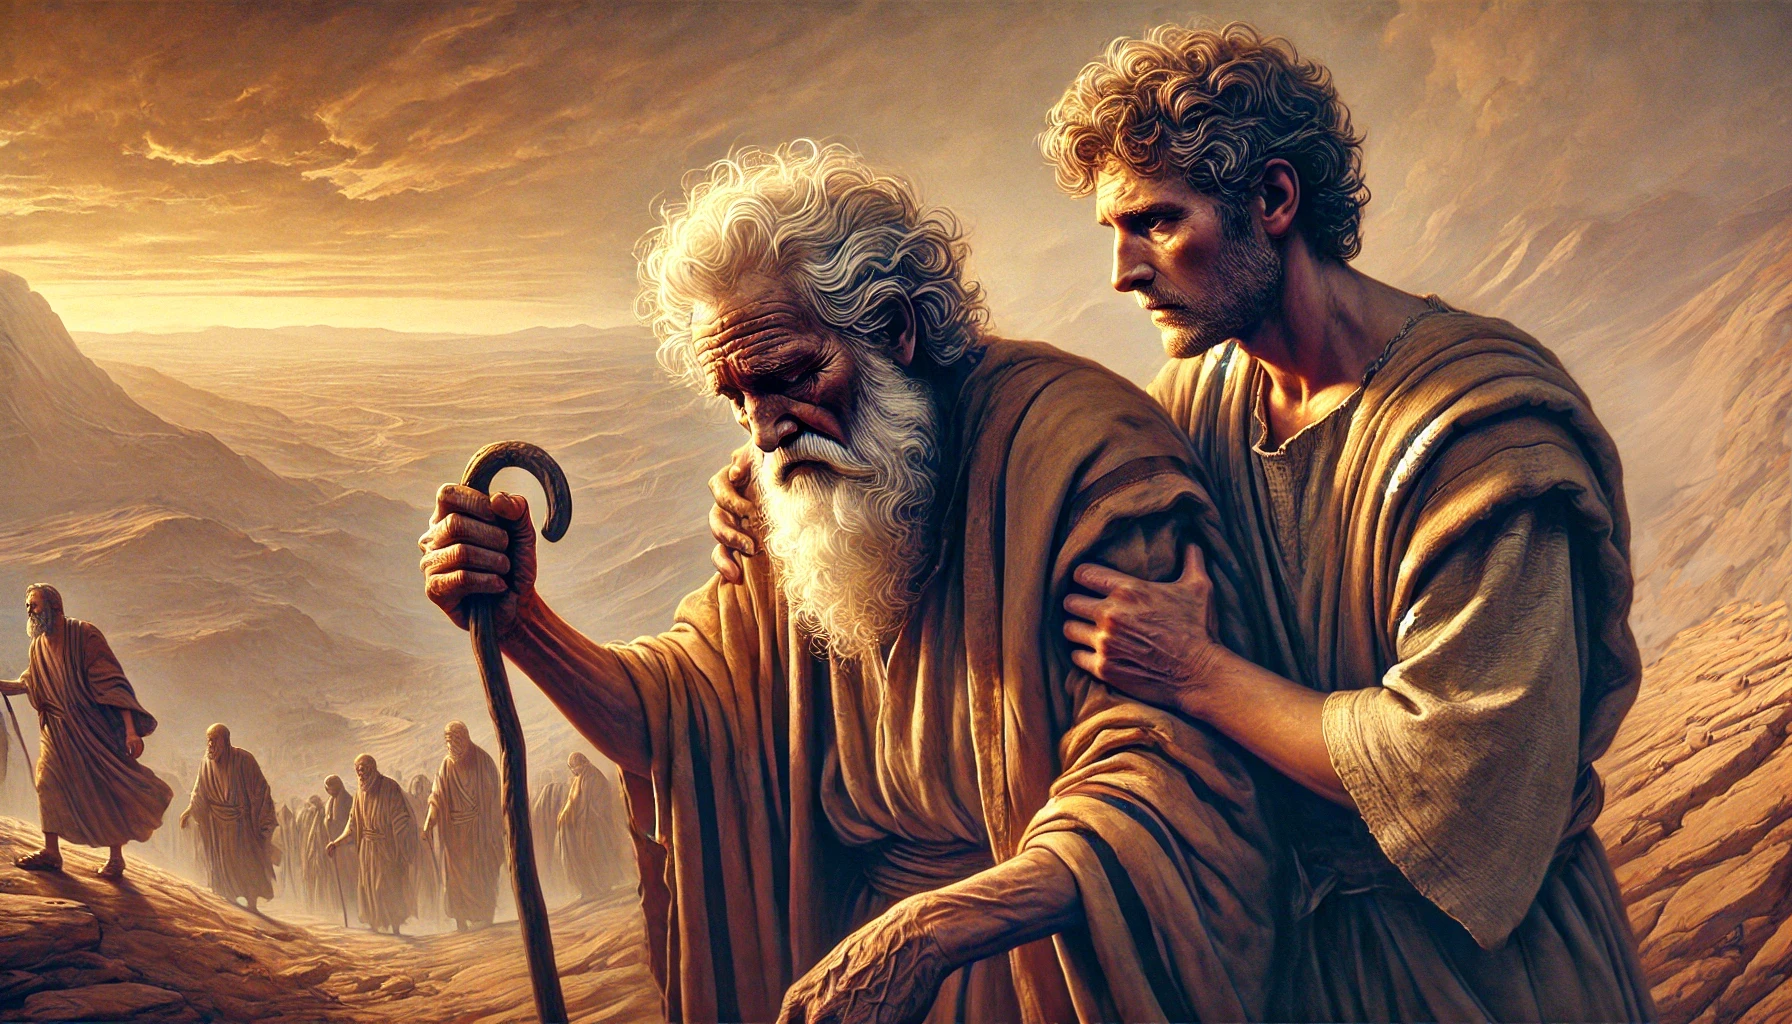
\includegraphics[width=0.7\linewidth]{graficas/deuteromonio}\\
	Moisés y Josué\\
\end{center}





\section*{Capítulo 1}


{Moisés recuerda a Israel las promesas de Jehová en Horeb } 



1:1 Estas son las palabras que habló Moisés a todo Israel a este lado del Jordán en el desierto, en el Arabá frente al Mar Rojo, entre Parán, Tofel, Labán, Hazerot y Dizahab.  
1:2 Once jornadas hay desde Horeb, camino del monte de Seir, hasta Cades-barnea.  
1:3 Y aconteció que a los cuarenta años, en el mes undécimo, el primero del mes, Moisés habló a los hijos de Israel conforme a todas las cosas que Jehová le había mandado acerca de ellos,  
1:4 después que derrotó a Sehón rey de los amorreos, el cual habitaba en Hesbón, y a Og rey de Basán que habitaba en Astarot en Edrei.  
1:5 De este lado del Jordán, en tierra de Moab, resolvió Moisés declarar esta ley, diciendo:  
1:6 Jehová nuestro Dios nos habló en Horeb, diciendo: Habéis estado bastante tiempo en este monte.  
1:7 Volveos e id al monte del amorreo y a todas sus comarcas, en el Arabá, en el monte, en los valles, en el Neguev, y junto a la costa del mar, a la tierra del cananeo, y al Líbano, hasta el gran río, el río Eufrates.  
1:8 Mirad, yo os he entregado la tierra; entrad y poseed la tierra que Jehová juró a vuestros padres Abraham, Isaac y Jacob, que les daría a ellos y a su descendencia después de ellos.  
Nombramiento de jueces   
1:9 En aquel tiempo yo os hablé diciendo: Yo solo no puedo llevaros.  
1:10 Jehová vuestro Dios os ha multiplicado, y he aquí hoy vosotros sois como las estrellas del cielo en multitud.  
1:11 ¡Jehová Dios de vuestros padres os haga mil veces más de lo que ahora sois, y os bendiga, como os ha prometido!  
1:12 ¿Cómo llevaré yo solo vuestras molestias, vuestras cargas y vuestros pleitos?  
1:13 Dadme de entre vosotros, de vuestras tribus, varones sabios y entendidos y expertos, para que yo los ponga por vuestros jefes.  
1:14 Y me respondisteis y dijisteis: Bueno es hacer lo que has dicho.  
1:15 Y tomé a los principales de vuestras tribus, varones sabios y expertos, y los puse por jefes sobre vosotros, jefes de millares, de centenas, de cincuenta y de diez, y gobernadores de vuestras tribus.  
1:16 Y entonces mandé a vuestros jueces, diciendo: Oíd entre vuestros hermanos, y juzgad justamente entre el hombre y su hermano, y el extranjero.  
1:17 No hagáis distinción de persona en el juicio; así al pequeño como al grande oiréis; no tendréis temor de ninguno, porque el juicio es de Dios; y la causa que os fuere difícil, la traeréis a mí, y yo la oiré.  
1:18 Os mandé, pues, en aquel tiempo, todo lo que habíais de hacer.  
Misión de los doce espías   
1:19 Y salidos de Horeb, anduvimos todo aquel grande y terrible desierto que habéis visto, por el camino del monte del amorreo, como Jehová nuestro Dios nos lo mandó; y llegamos hasta Cades- barnea.  
1:20 Entonces os dije: Habéis llegado al monte del amorreo, el cual Jehová nuestro Dios nos da.  
1:21 Mira, Jehová tu Dios te ha entregado la tierra; sube y toma posesión de ella, como Jehová el Dios de tus padres te ha dicho; no temas ni desmayes.  
1:22 Y vinisteis a mí todos vosotros, y dijisteis: Enviemos varones delante de nosotros que nos reconozcan la tierra, y a su regreso nos traigan razón del camino por donde hemos de subir, y de las ciudades adonde hemos de llegar.  
1:23 Y el dicho me pareció bien; y tomé doce varones de entre vosotros, un varón por cada tribu.  
1:24 Y se encaminaron, y subieron al monte, y llegaron hasta el valle de Escol, y reconocieron la tierra.  
1:25 Y tomaron en sus manos del fruto del país, y nos lo trajeron, y nos dieron cuenta, y dijeron: Es buena la tierra que Jehová nuestro Dios nos da.  
1:26 Sin embargo, no quisisteis subir, antes fuisteis rebeldes al mandato de Jehová vuestro Dios;  
1:27 y murmurasteis en vuestras tiendas, diciendo: Porque Jehová nos aborrece, nos ha sacado de tierra de Egipto, para entregarnos en manos del amorreo para destruirnos.  
1:28 ¿A dónde subiremos? Nuestros hermanos han atemorizado nuestro corazón, diciendo: Este pueblo es mayor y más alto que nosotros, las ciudades grandes y amuralladas hasta el cielo; y también vimos allí a los hijos de Anac. 
1:29 Entonces os dije: No temáis, ni tengáis miedo de ellos.  
1:30 Jehová vuestro Dios, el cual va delante de vosotros, él peleará por vosotros, conforme a todas las cosas que hizo por vosotros en Egipto delante de vuestros ojos.  
1:31 Y en el desierto has visto que Jehová tu Dios te ha traído, como trae el hombre a su hijo, por todo el camino que habéis andado, hasta llegar a este lugar.  
1:32 Y aun con esto no creísteis a Jehová vuestro Dios, 
1:33 quien iba delante de vosotros por el camino para reconoceros el lugar donde habíais de acampar, con fuego de noche para mostraros el camino por donde anduvieseis, y con nube de día.  
Dios castiga a Israel   
1:34 Y oyó Jehová la voz de vuestras palabras, y se enojó, y juró diciendo:  
1:35 No verá hombre alguno de estos, de esta mala generación, la buena tierra que juré que había de dar a vuestros padres,  
1:36 excepto Caleb hijo de Jefone; él la verá, y a él le daré la tierra que pisó, y a sus hijos; porque ha seguido fielmente a Jehová.  
1:37 También contra mí se airó Jehová por vosotros, y me dijo: Tampoco tú entrarás allá.  
1:38 Josué hijo de Nun, el cual te sirve, él entrará allá; anímale, porque él la hará heredar a Israel.  
1:39 Y vuestros niños, de los cuales dijisteis que servirían de botín, y vuestros hijos que no saben hoy lo bueno ni lo malo, ellos entrarán allá, y a ellos la daré, y ellos la heredarán.  
1:40 Pero vosotros volveos e id al desierto, camino del Mar Rojo.  
La derrota en Horma   
1:1:41 Entonces respondisteis y me dijisteis: Hemos pecado contra Jehová; nosotros subiremos y pelearemos, conforme a todo lo que Jehová nuestro Dios nos ha mandado. Y os armasteis cada uno con sus armas de guerra, y os preparasteis para subir al monte.  
1:42 Y Jehová me dijo: Diles: No subáis, ni peleéis, pues no estoy entre vosotros; para que no seáis derrotados por vuestros enemigos.  
1:43 Y os hablé, y no disteis oído; antes fuisteis rebeldes al mandato de Jehová, y persistiendo con altivez subisteis al monte.  
1:44 Pero salió a vuestro encuentro el amorreo, que habitaba en aquel monte, y os persiguieron como hacen las avispas, y os derrotaron en Seir, hasta Horma.  
1:45 Y volvisteis y llorasteis delante de Jehová, pero Jehová no escuchó vuestra voz, ni os prestó oído.  
1:46 Y estuvisteis en Cades por muchos días, los días que habéis estado allí.  
\section*{Capítulo 2}
Los años en el desierto  

2:1 Luego volvimos y salimos al desierto, camino del Mar Rojo, como Jehová me había dicho; y rodeamos el monte de Seir por mucho tiempo.  
2:2 Y Jehová me habló, diciendo:  
2:3 Bastante habéis rodeado este monte; volveos al norte.  
2:4 Y manda al pueblo, diciendo: Pasando vosotros por el territorio de vuestros hermanos los hijos de Esaú, que habitan en Seir, ellos tendrán miedo de vosotros; mas vosotros guardaos mucho.  
2:5 No os metáis con ellos, porque no os daré de su tierra ni aun lo que cubre la planta de un pie; porque yo he dado por heredad a Esaú el monte de Seir.  
2:6 Compraréis de ellos por dinero los alimentos, y comeréis; y también compraréis de ellos el agua, y beberéis;  
2:7 pues Jehová tu Dios te ha bendecido en toda obra de tus manos; él sabe que andas por este gran desierto; estos cuarenta años Jehová tu Dios ha estado contigo, y nada te ha faltado.  
2:8 Y nos alejamos del territorio de nuestros hermanos los hijos de Esaú, que habitaban en Seir, por el camino del Arabá desde Elat y Ezión-geber; y volvimos, y tomamos el camino del desierto de Moab.  
2:9 Y Jehová me dijo: No molestes a Moab, ni te empeñes con ellos en guerra, porque no te daré posesión de su tierra; porque yo he dado a Ar por heredad a los hijos de Lot.  
2:10 (Los emitas habitaron en ella antes, pueblo grande y numeroso, y alto como los hijos de Anac.  
2:11 Por gigantes eran ellos tenidos también, como los hijos de Anac; y los moabitas los llaman emitas.  
2:12 Y en Seir habitaron antes los horeos, a los cuales echaron los hijos de Esaú; y los arrojaron de su presencia, y habitaron en lugar de ellos, como hizo Israel en la tierra que les dio Jehová por posesión.)  
2:13 Levantaos ahora, y pasad el arroyo de Zered. Y pasamos el arroyo de Zered.  
2:14 Y los días que anduvimos de Cades-barnea hasta cuando pasamos el arroyo de Zered fueron treinta y ocho años; hasta que se acabó toda la generación de los hombres de guerra de en medio del campamento, como Jehová les había jurado. 
2:15 Y también la mano de Jehová vino sobre ellos para destruirlos de en medio del campamento, hasta acabarlos.  
2:16 Y aconteció que después que murieron todos los hombres de guerra de entre el pueblo,  
2:17 Jehová me habló, diciendo:  
2:18 Tú pasarás hoy el territorio de Moab, a Ar.  
2:19 Y cuando te acerques a los hijos de Amón, no los molestes, ni contiendas con ellos; porque no te daré posesión de la tierra de los hijos de Amón, pues a los hijos de Lot la he dado por heredad.  
2:20 (Por tierra de gigantes fue también ella tenida; habitaron en ella gigantes en otro tiempo, a los cuales los amonitas llamaban zomzomeos;  
2:21 pueblo grande y numeroso, y alto, como los hijos de Anac; a los cuales Jehová destruyó delante de los amonitas. Estos sucedieron a aquéllos, y habitaron en su lugar,  
2:22 como hizo Jehová con los hijos de Esaú que habitaban en Seir, delante de los cuales destruyó a los horeos; y ellos sucedieron a éstos, y habitaron en su lugar hasta hoy.  
2:23 Y a los aveos que habitaban en aldeas hasta Gaza, los caftoreos que salieron de Caftor los destruyeron, y habitaron en su lugar.)  
2:24 Levantaos, salid, y pasad el arroyo de Arnón; he aquí he entregado en tu mano a Sehón rey de Hesbón, amorreo, y a su tierra; comienza a tomar posesión de ella, y entra en guerra con él.  
2:25 Hoy comenzaré a poner tu temor y tu espanto sobre los pueblos debajo de todo el cielo, los cuales oirán tu fama, y temblarán y se angustiarán delante de ti.  
Israel derrota a Sehón   
2:26 Y envié mensajeros desde el desierto de Cademot a Sehón rey de Hesbón con palabras de paz, diciendo:  
2:27 Pasaré por tu tierra por el camino; por el camino iré, sin apartarme ni a diestra ni a siniestra.  
2:28 La comida me venderás por dinero, y comeré; el agua también me darás por dinero, y beberé; solamente pasaré a pie,  
2:29 como lo hicieron conmigo los hijos de Esaú que habitaban en Seir, y los moabitas que habitaban en Ar; hasta que cruce el Jordán a la tierra que nos da Jehová nuestro Dios.  
2:30 Mas Sehón rey de Hesbón no quiso que pasásemos por el territorio suyo; porque Jehová tu Dios había endurecido su espíritu, y obstinado su corazón para entregarlo en tu mano, como hasta hoy.  
2:31 Y me dijo Jehová: He aquí yo he comenzado a entregar delante de ti a Sehón y a su tierra; comienza a tomar posesión de ella para que la heredes.  
2:32 Y nos salió Sehón al encuentro, él y todo su pueblo, para pelear en Jahaza.  
2:33 Mas Jehová nuestro Dios lo entregó delante de nosotros; y lo derrotamos a él y a sus hijos, y a todo su pueblo.  
2:34 Tomamos entonces todas sus ciudades, y destruimos todas las ciudades, hombres, mujeres y niños; no dejamos ninguno.  
2:35 Solamente tomamos para nosotros los ganados, y los despojos de las ciudades que habíamos tomado.  
2:36 Desde Aroer, que está junto a la ribera del arroyo de Arnón, y la ciudad que está en el valle, hasta Galaad, no hubo ciudad que escapase de nosotros; todas las entregó Jehová nuestro Dios en nuestro poder.  
2:37 Solamente a la tierra de los hijos de Amón no llegamos; ni a todo lo que está a la orilla del arroyo de Jaboc ni a las ciudades del monte, ni a lugar alguno que Jehová nuestro Dios había prohibido.  
\section*{Capítulo 3}
Israel derrota a Og rey de Basán  

3:1 Volvimos, pues, y subimos camino de Basán, y nos salió al encuentro Og rey de Basán para pelear, él y todo su pueblo, en Edrei.  
3:2 Y me dijo Jehová: No tengas temor de él, porque en tu mano he entregdo a él y a todo su pueblo, con su tierra; y harás con él como hiciste con Sehón rey amorreo, que habitaba en Hesbón.  
3:3 Y Jehová nuestro Dios entregó también en nuestra mano a Og rey de Basán, y a todo su pueblo, al cual derrotamos hasta acabar con todos.  
3:4 Y tomamos entonces todas sus ciudades; no quedó ciudad que no les tomásemos; sesenta ciudades, toda la tierra de Argob, del reino de Og en Basán.  
3:5 Todas estas eran ciudades fortificadas con muros altos, con puertas y barras, sin contar otras muchas ciudades sin muro.  
3:6 Y las destruimos, como hicimos a Sehón rey de Hesbón, matando en toda ciudad a hombres, mujeres y niños.  
3:7 Y tomamos para nosotros todo el ganado, y los despojos de las ciudades.  
3:8 También tomamos en aquel tiempo la tierra desde el arroyo de Arnón hasta el monte de Hermón, de manos de los dos reyes amorreos que estaban a este lado del Jordán.  
3:9 (Los sidonios llaman a Hermón, Sirión; y los amorreos, Senir.)  
3:10 Todas las ciudades de la llanura, y todo Galaad, y todo Basán hasta Salca y Edrei, ciudades del reino de Og en Basán.  
3:11 Porque únicamente Og rey de Basán había quedado del resto de los gigantes. Su cama, una cama de hierro, ¿no está en Rabá de los hijos de Amón? La longitud de ella es de nueve codos, y su anchura de cuatro codos, según el codo de un hombre.  
Rubén, Gad y la media tribu de Manasés se establecen al oriente del Jordán  

3:12 Y esta tierra que heredamos en aquel tiempo, desde Aroer, que está junto al arroyo de Arnón, y la mitad del monte de Galaad con sus ciudades, la di a los rubenitas y a los gaditas;  
3:13 y el resto de Galaad, y todo Basán, del reino de Og, toda la tierra de Argob, que se llamaba la tierra de los gigantes, lo di a la media tribu de Manasés.  
3:14 Jair hijo de Manasés tomó toda la tierra de Argob hasta el límite con Gesur y Maaca, y la llamó por su nombre, Basán- havot-jair, hasta hoy.  
3:15 Y Galaad se lo di a Maquir.  
3:16 Y a los rubenitas y gaditas les di de Galaad hasta el arroyo de Arnón, teniendo por límite el medio del valle, hasta el arroyo de Jaboc, el cual es límite de los hijos de Amón;  
3:17 también el Arabá, con el Jordán como límite desde Cineret hasta el mar del Arabá, el Mar Salado, al pie de las laderas del Pisga al oriente.  
3:18 Y os mandé entonces, diciendo: Jehová vuestro Dios os ha dado esta tierra por heredad; pero iréis armados todos los valientes delante de vuestros hermanos los hijos de Israel.  
3:19 Solamente vuestras mujeres, vuestros hijos y vuestros ganados (yo sé que tenéis mucho ganado), quedarán en las ciudades que os he dado,  
3:20 hasta que Jehová dé reposo a vuestros hermanos, así como a vosotros, y hereden ellos también la tierra que Jehová vuestro Dios les da al otro lado del Jordán; entonces os volveréis cada uno a la heredad que yo os he dado.  
3:21 Ordené también a Josué en aquel tiempo, diciendo: Tus ojos vieron todo lo que Jehová vuestro Dios ha hecho a aquellos dos reyes; así hará Jehová a todos los reinos a los cuales pasarás tú.  
3:22 No los temáis; porque Jehová vuestro Dios, él es el que pelea por vosotros.  
No se le permite a Moisés entrar a Canaán  
3:23 Y oré a Jehová en aquel tiempo, diciendo:  
3:24 Señor Jehová, tú has comenzado a mostrar a tu siervo tu grandeza, y tu mano poderosa; porque ¿qué dios hay en el cielo ni en la tierra que haga obras y proezas como las tuyas?  
3:25 Pase yo, te ruego, y vea aquella tierra buena que está más allá del Jordán, aquel buen monte, y el Líbano.  
3:26 Pero Jehová se había enojado contra mí a causa de vosotros, por lo cual no me escuchó; y me dijo Jehová: Basta, no me hables más de este asunto.  
3:27 Sube a la cumbre del Pisga y alza tus ojos al oeste, y al norte, y al sur, y al este, y mira con tus propios ojos; porque no pasarás el Jordán.  
3:28 Y manda a Josué, y anímalo, y fortalécelo; porque él ha de pasar delante de este pueblo, y él les hará heredar la tierra que verás.  
3:29 Y paramos en el valle delante de Bet-peor.  
\section*{Capítulo 4 }
Moisés exhorta a la obediencia  

4:1 Ahora, pues, oh Israel, oye los estatutos y decretos que yo os enseño, para que los ejecutéis, y viváis, y entréis y poseáis la tierra que Jehová el Dios de vuestros padres os da.  
4:2 No añadiréis a la palabra que yo os mando, ni disminuiréis de ella, para que guardéis los mandamientos de Jehová vuestro Dios que yo os ordene.  
4:3 Vuestros ojos vieron lo que hizo Jehová con motivo de Baal- peor; que a todo hombre que fue en pos de Baal-peor destruyó Jehová tu Dios de en medio de ti.  
4:4 Mas vosotros que seguisteis a Jehová vuestro Dios, todos estáis vivos hoy.  
4:5 Mirad, yo os he enseñado estatutos y decretos, como Jehová mi Dios me mandó, para que hagáis así en medio de la tierra en la cual entráis para tomar posesión de ella.  
4:6 Guardadlos, pues, y ponedlos por obra; porque esta es vuestra sabiduría y vuestra inteligencia ante los ojos de los pueblos, los cuales oirán todos estos estatutos, y dirán: Ciertamente pueblo sabio y entendido, nación grande es esta.  
4:7 Porque ¿qué nación grande hay que tenga dioses tan cercanos a ellos como lo está Jehová nuestro Dios en todo cuanto le pedimos?  
4:8 Y ¿qué nación grande hay que tenga estatutos y juicios justos como es toda esta ley que yo pongo hoy delante de vosotros?  
La experiencia de Israel en Horeb  
4:9 Por tanto, guárdate, y guarda tu alma con diligencia, para que no te olvides de las cosas que tus ojos han visto, ni se aparten de tu corazón todos los días de tu vida; antes bien, las enseñarás a tus hijos, y a los hijos de tus hijos.  
4:10 El día que estuviste delante de Jehová tu Dios en Horeb, cuando Jehová me dijo: Reúneme el pueblo, para que yo les haga oír mis palabras, las cuales aprenderán, para temerme todos los días que vivieren sobre la tierra, y las enseñarán a sus hijos;  
4:11 y os acercasteis y os pusisteis al pie del monte; y el monte ardía en fuego hasta en medio de los cielos con tinieblas, nube y oscuridad;  
4:12 y habló Jehová con vosotros de en medio del fuego; oísteis la voz de sus palabras, mas a excepción de oír la voz, ninguna figura visteis.  
4:13 Y él os anunció su pacto, el cual os mandó poner por obra; los diez mandamientos, y los escribió en dos tablas de piedra. 
4:14 A mí también me mandó Jehová en aquel tiempo que os enseñase los estatutos y juicios, para que los pusieseis por obra en la tierra a la cual pasáis a tomar posesión de ella.  
Advertencia contra la idolatría  
4:15 Guardad, pues, mucho vuestras almas; pues ninguna figura visteis el día que Jehová habló con vosotros de en medio del fuego;  
4:16 para que no os corrompáis y hagáis para vosotros escultura, imagen de figura alguna, efigie de varón o hembra,  
4:17 figura de animal alguno que está en la tierra, figura de ave alguna alada que vuele por el aire,  
4:18 figura de ningún animal que se arrastre sobre la tierra, figura de pez alguno que haya en el agua debajo de la tierra.  
4:19 No sea que alces tus ojos al cielo, y viendo el sol y la luna y las estrellas, y todo el ejército del cielo, seas impulsado, y te inclines a ellos y les sirvas; porque Jehová tu Dios los ha concedido a todos los pueblos debajo de todos los cielos.  
4:20 Pero a vosotros Jehová os tomó, y os ha sacado del horno de hierro, de Egipto, para que seáis el pueblo de su heredad como en este día.  
4:21 Y Jehová se enojó contra mí por causa de vosotros, y juró que yo no pasaría el Jordán, ni entraría en la buena tierra que Jehová tu Dios te da por heredad.  
4:22 Así que yo voy a morir en esta tierra, y no pasaré el Jordán; mas vosotros pasaréis, y poseeréis aquella buena tierra.  
4:23 Guardaos, no os olvidéis del pacto de Jehová vuestro Dios, que él estableció con vosotros, y no os hagáis escultura o imagen de ninguna cosa que Jehová tu Dios te ha prohibido.  
4:24 Porque Jehová tu Dios es fuego consumidor, Dios celoso.  
4:25 Cuando hayáis engendrado hijos y nietos, y hayáis envejecido en la tierra, si os corrompiereis e hiciereis escultura o imagen de cualquier cosa, e hiciereis lo malo ante los ojos de Jehová vuestro Dios, para enojarlo;  
4:26 yo pongo hoy por testigos al cielo y a la tierra, que pronto pereceréis totalmente de la tierra hacia la cual pasáis el Jordán para tomar posesión de ella; no estaréis en ella largos días sin que seáis destruidos.  
4:27 Y Jehová os esparcirá entre los pueblos, y quedaréis pocos en número entre las naciones a las cuales os llevará Jehová.  
4:28 Y serviréis allí a dioses hechos de manos de hombres, de madera y piedra, que no ven, ni oyen, ni comen, ni huelen.  
4:29 Mas si desde allí buscares a Jehová tu Dios, lo hallarás, si lo buscares de todo tu corazón y de toda tu alma.  
4:30 Cuando estuvieres en angustia, y te alcanzaren todas estas cosas, si en los postreros días te volvieres a Jehová tu Dios, y oyeres su voz;  
4:31 porque Dios misericordioso es Jehová tu Dios; no te dejará, ni te destruirá, ni se olvidará del pacto que les juró a tus padres.  
4:32 Porque pregunta ahora si en los tiempos pasados que han sido antes de ti, desde el día que creó Dios al hombre sobre la tierra, si desde un extremo del cielo al otro se ha hecho cosa semejante a esta gran cosa, o se haya oído otra como ella.  
4:33 ¿Ha oído pueblo alguno la voz de Dios, hablando de en medio del fuego, como tú la has oído, sin perecer?  
4:34 ¿O ha intentado Dios venir a tomar para sí una nación de en medio de otra nación, con pruebas, con señales, con milagros y con guerra, y mano poderosa y brazo extendido, y hechos aterradores como todo lo que hizo con vosotros Jehová vuestro Dios en Egipto ante tus ojos?  
4:35 A ti te fue mostrado, para que supieses que Jehová es Dios, y no hay otro fuera de él.  
4:36 Desde los cielos te hizo oír su voz, para enseñarte; y sobre la tierra te mostró su gran fuego, y has oído sus palabras de en medio del fuego.  
4:37 Y por cuanto él amó a tus padres, escogió a su descendencia después de ellos, y te sacó de Egipto con su presencia y con su gran poder,  
4:38 para echar de delante de tu presencia naciones grandes y más fuertes que tú, y para introducirte y darte su tierra por heredad, como hoy.  
4:39 Aprende pues, hoy, y reflexiona en tu corazón que Jehová es Dios arriba en el cielo y abajo en la tierra, y no hay otro.  
4:40 Y guarda sus estatutos y sus mandamientos, los cuales yo te mando hoy, para que te vaya bien a ti y a tus hijos después de ti, y prolongues tus días sobre la tierra que Jehová tu Dios te da para siempre.  
Las ciudades de refugio al oriente del Jordán  
4:41 Entonces apartó Moisés tres ciudades a este lado del Jordán al nacimiento del sol,  
4:42 para que huyese allí el homicida que matase a su prójimo sin intención, sin haber tenido enemistad con él nunca antes; y que huyendo a una de estas ciudades salvase su vida:  
4:43 Beser en el desierto, en tierra de la llanura, para los rubenitas; Ramot en Galaad para los gaditas, y Golán en Basán para los de Manasés.  
Moisés recapitula la promulgación de la ley  
4:44 Esta, pues, es la ley que Moisés puso delante de los hijos de Israel.  
4:45 Estos son los testimonios, los estatutos y los decretos que habló Moisés a los hijos de Israel cuando salieron de Egipto;  
4:46 a este lado del Jordán, en el valle delante de Bet-peor, en la tierra de Sehón rey de los amorreos que habitaba en Hesbón, al cual derrotó Moisés con los hijos de Israel, cuando salieron de Egipto;  
4:47 y poseyeron su tierra, y la tierra de Og rey de Basán; dos reyes de los amorreos que estaban de este lado del Jordán, al oriente. 
4:48 Desde Aroer, que está junto a la ribera del arroyo de Arnón, hasta el monte de Sion, que es Hermón; 
4:49 y todo el Arabá de este lado del Jordán, al oriente, hasta el mar del Arabá, al pie de las laderas del Pisga.  
\section*{Capítulo 5 }
Los Diez Mandamientos   

5:1 Llamó Moisés a todo Israel y les dijo: Oye, Israel, los estatutos y decretos que yo pronuncio hoy en vuestros oídos; aprendedlos, y guardadlos, para ponerlos por obra.  
5:2 Jehová nuestro Dios hizo pacto con nosotros en Horeb.  
5:3 No con nuestros padres hizo Jehová este pacto, sino con nosotros todos los que estamos aquí hoy vivos.  
5:4 Cara a cara habló Jehová con vosotros en el monte de en medio del fuego.  
5:5 Yo estaba entonces entre Jehová y vosotros, para declararos la palabra de Jehová; porque vosotros tuvisteis temor del fuego, y no subisteis al monte. Dijo:  
5:6 Yo soy Jehová tu Dios, que te saqué de tierra de Egipto, de casa de servidumbre.  
5:7 No tendrás dioses ajenos delante de mí.  
5:8 No harás para ti escultura, ni imagen alguna de cosa que está arriba en los cielos, ni abajo en la tierra, ni en las aguas debajo de la tierra.  
5:9 No te inclinarás a ellas ni las servirás; porque yo soy Jehová tu Dios, fuerte, celoso, que visito la maldad de los padres sobre los hijos hasta la tercera y cuarta generación de los que me aborrecen,  
5:10 y que hago misericordia a millares, a los que me aman y guardan mis mandamientos.  
5:11 No tomarás el nombre de Jehová tu Dios en vano; porque Jehová no dará por inocente al que tome su nombre en vano.  
5:12 Guardarás el día de reposo para santificarlo, como Jehová tu Dios te ha mandado. 
5:13 Seis días trabajarás, y harás toda tu obra;  
5:14 mas el séptimo día es reposo a Jehová tu Dios; ninguna obra harás tú, ni tu hijo, ni tu hija, ni tu siervo, ni tu sierva, ni tu buey, ni tu asno, ni ningún animal tuyo, ni el extranjero que está dentro de tus puertas, para que descanse tu siervo y tu sierva como tú.  
5:15 Acuérdate que fuiste siervo en tierra de Egipto, y que Jehová tu Dios te sacó de allá con mano fuerte y brazo extendido; por lo cual Jehová tu Dios te ha mandado que guardes el día de reposo.  
5:16 Honra a tu padre y a tu madre, como Jehová tu Dios te ha mandado, para que sean prolongados tus días, y para que te vaya bien sobre la tierra que Jehová tu Dios te da.  
5:17 No matarás. 
5:18 No cometerás adulterio.  
5:19 No hurtarás. 
5:20 No dirás falso testimonio contra tu prójimo.  
5:21 No codiciarás la mujer de tu prójimo, ni desearás la casa de tu prójimo, ni su tierra, ni su siervo, ni su sierva, ni su buey, ni su asno, ni cosa alguna de tu prójimo.  
El terror del pueblo   
5:22 Estas palabras habló Jehová a toda vuestra congregación en el monte, de en medio del fuego, de la nube y de la oscuridad, a gran voz; y no añadió más. Y las escribió en dos tablas de piedra, las cuales me dio a mí.  
5:23 Y aconteció que cuando vosotros oísteis la voz de en medio de las tinieblas, y visteis al monte que ardía en fuego, vinisteis a mí, todos los príncipes de vuestras tribus, y vuestros ancianos,  
5:24 y dijisteis: He aquí Jehová nuestro Dios nos ha mostrado su gloria y su grandeza, y hemos oído su voz de en medio del fuego; hoy hemos visto que Jehová habla al hombre, y éste aún vive.  
5:25 Ahora, pues, ¿por qué vamos a morir? Porque este gran fuego nos consumirá; si oyéremos otra vez la voz de Jehová nuestro Dios, moriremos.  
5:26 Porque ¿qué es el hombre, para que oiga la voz del Dios viviente que habla de en medio del fuego, como nosotros la oímos, y aún viva?  
5:27 Acércate tú, y oye todas las cosas que dijere Jehová nuestro Dios; y tú nos dirás todo lo que Jehová nuestro Dios te dijere, y nosotros oiremos y haremos.  
5:28 Y oyó Jehová la voz de vuestras palabras cuando me hablabais, y me dijo Jehová: He oído la voz de las palabras de este pueblo, que ellos te han hablado; bien está todo lo que han dicho.  
5:29 ¡Quién diera que tuviesen tal corazón, que me temiesen y guardasen todos los días todos mis mandamientos, para que a ellos y a sus hijos les fuese bien para siempre!  
5:30 Ve y diles: Volveos a vuestras tiendas.  
5:31 Y tú quédate aquí conmigo, y te diré todos los mandamientos y estatutos y decretos que les enseñarás, a fin de que los pongan ahora por obra en la tierra que yo les doy por posesión.  
5:32 Mirad, pues, que hagáis como Jehová vuestro Dios os ha mandado; no os apartéis a diestra ni a siniestra.  
5:33 Andad en todo el camino que Jehová vuestro Dios os ha mandado, para que viváis y os vaya bien, y tengáis largos días en la tierra que habéis de poseer.  
\section*{Capítulo 6 }
El gran mandamiento  

6:1 Estos, pues, son los mandamientos, estatutos y decretos que Jehová vuestro Dios mandó que os enseñase, para que los pongáis por obra en la tierra a la cual pasáis vosotros para tomarla;  
6:2 para que temas a Jehová tu Dios, guardando todos sus estatutos y sus mandamientos que yo te mando, tú, tu hijo, y el hijo de tu hijo, todos los días de tu vida, para que tus días sean prolongados.  
6:3 Oye, pues, oh Israel, y cuida de ponerlos por obra, para que te vaya bien en la tierra que fluye leche y miel, y os multipliquéis, como te ha dicho Jehová el Dios de tus padres.  
6:4 Oye, Israel: Jehová nuestro Dios, Jehová uno es.  
6:5 Y amarás a Jehová tu Dios de todo tu corazón, y de toda tu alma, y con todas tus fuerzas.  
6:6 Y estas palabras que yo te mando hoy, estarán sobre tu corazón;  
6:7 y las repetirás a tus hijos, y hablarás de ellas estando en tu casa, y andando por el camino, y al acostarte, y cuando te levantes.  
6:8 Y las atarás como una señal en tu mano, y estarán como frontales entre tus ojos;  
6:9 y las escribirás en los postes de tu casa, y en tus puertas.  
Exhortaciones a la obediencia  
6:10 Cuando Jehová tu Dios te haya introducido en la tierra que juró a tus padres Abraham, Isaac y Jacob que te daría, en ciudades grandes y buenas que tú no edificaste,  
6:11 y casas llenas de todo bien, que tú no llenaste, y cisternas cavadas que tú no cavaste, viñas y olivares que no plantaste, y luego que comas y te sacies,  
6:12 cuídate de no olvidarte de Jehová, que te sacó de la tierra de Egipto, de casa de servidumbre.  
6:13 A Jehová tu Dios temerás, y a él solo servirás, y por su nombre jurarás.  
6:14 No andaréis en pos de dioses ajenos, de los dioses de los pueblos que están en vuestros contornos;  
6:15 porque el Dios celoso, Jehová tu Dios, en medio de ti está; para que no se inflame el furor de Jehová tu Dios contra ti, y te destruya de sobre la tierra.  
6:16 No tentaréis a Jehová vuestro Dios, como lo tentasteis en Masah.  
6:17 Guardad cuidadosamente los mandamientos de Jehová vuestro Dios, y sus testimonios y sus estatutos que te ha mandado.  
6:18 Y haz lo recto y bueno ante los ojos de Jehová, para que te vaya bien, y entres y poseas la buena tierra que Jehová juró a tus padres;  
6:19 para que él arroje a tus enemigos de delante de ti, como Jehová ha dicho.  
6:20 Mañana cuando te preguntare tu hijo, diciendo: ¿Qué significan los testimonios y estatutos y decretos que Jehová nuestro Dios os mandó?  
6:21 entonces dirás a tu hijo: Nosotros éramos siervos de Faraón en Egipto, y Jehová nos sacó de Egipto con mano poderosa.  
6:22 Jehová hizo señales y milagros grandes y terribles en Egipto, sobre Faraón y sobre toda su casa, delante de nuestros ojos;  
6:23 y nos sacó de allá, para traernos y darnos la tierra que juró a nuestros padres.  
6:24 Y nos mandó Jehová que cumplamos todos estos estatutos, y que temamos a Jehová nuestro Dios, para que nos vaya bien todos los días, y para que nos conserve la vida, como hasta hoy.  
6:25 Y tendremos justicia cuando cuidemos de poner por obra todos estos mandamientos delante de Jehová nuestro Dios, como él nos ha mandado.  
\section*{Capítulo 7 }
Advertencias contra la idolatría de Canaán   

7:1 Cuando Jehová tu Dios te haya introducido en la tierra en la cual entrarás para tomarla, y haya echado de delante de ti a muchas naciones, al heteo, al gergeseo, al amorreo, al cananeo, al ferezeo, al heveo y al jebuseo, siete naciones mayores y más poderosas que tú,  
7:2 y Jehová tu Dios las haya entregado delante de ti, y las hayas derrotado, las destruirás del todo; no harás con ellas alianza, ni tendrás de ellas misericordia.  
7:3 Y no emparentarás con ellas; no darás tu hija a su hijo, ni tomarás a su hija para tu hijo.  
7:4 Porque desviará a tu hijo de en pos de mí, y servirán a dioses ajenos; y el furor de Jehová se encenderá sobre vosotros, y te destruirá pronto.  
7:5 Mas así habéis de hacer con ellos: sus altares destruiréis, y quebraréis sus estatuas, y destruiréis sus imágenes de Asera, y quemaréis sus esculturas en el fuego.  
Un pueblo santo para Jehová  
7:6 Porque tú eres pueblo santo para Jehová tu Dios; Jehová tu Dios te ha escogido para serle un pueblo especial, más que todos los pueblos que están sobre la tierra.  
7:7 No por ser vosotros más que todos los pueblos os ha querido Jehová y os ha escogido, pues vosotros erais el más insignificante de todos los pueblos;  
7:8 sino por cuanto Jehová os amó, y quiso guardar el juramento que juró a vuestros padres, os ha sacado Jehová con mano poderosa, y os ha rescatado de servidumbre, de la mano de Faraón rey de Egipto.  
7:9 Conoce, pues, que Jehová tu Dios es Dios, Dios fiel, que guarda el pacto y la misericordia a los que le aman y guardan sus mandamientos, hasta mil generaciones;  
7:10 y que da el pago en persona al que le aborrece, destruyéndolo; y no se demora con el que le odia, en persona le dará el pago.  
7:11 Guarda, por tanto, los mandamientos, estatutos y decretos que yo te mando hoy que cumplas.  
Bendiciones de la obediencia   
7:12 Y por haber oído estos decretos y haberlos guardado y puesto por obra, Jehová tu Dios guardará contigo el pacto y la misericordia que juró a tus padres.  
7:13 Y te amará, te bendecirá y te multiplicará, y bendecirá el fruto de tu vientre y el fruto de tu tierra, tu grano, tu mosto, tu aceite, la cría de tus vacas, y los rebaños de tus ovejas, en la tierra que juró a tus padres que te daría.  
7:14 Bendito serás más que todos los pueblos; no habrá en ti varón ni hembra estéril, ni en tus ganados.  
7:15 Y quitará Jehová de ti toda enfermedad; y todas las malas plagas de Egipto, que tú conoces, no las pondrá sobre ti, antes las pondrá sobre todos los que te aborrecieren.  
7:16 Y consumirás a todos los pueblos que te da Jehová tu Dios; no los perdonará tu ojo, ni servirás a sus dioses, porque te será tropiezo.  
7:17 Si dijeres en tu corazón: Estas naciones son mucho más numerosas que yo; ¿cómo las podré exterminar?  
7:18 no tengas temor de ellas; acuérdate bien de lo que hizo Jehová tu Dios con Faraón y con todo Egipto;  
7:19 de las grandes pruebas que vieron tus ojos, y de las señales y milagros, y de la mano poderosa y el brazo extendido con que Jehová tu Dios te sacó; así hará Jehová tu Dios con todos los pueblos de cuya presencia tú temieres.  
7:20 También enviará Jehová tu Dios avispas sobre ellos, hasta que perezcan los que quedaren y los que se hubieren escondido de delante de ti.  
7:21 No desmayes delante de ellos, porque Jehová tu Dios está en medio de ti, Dios grande y temible.  
7:22 Y Jehová tu Dios echará a estas naciones de delante de ti poco a poco; no podrás acabar con ellas en seguida, para que las fieras del campo no se aumenten contra ti.  
7:23 Mas Jehová tu Dios las entregará delante de ti, y él las quebrantará con grande destrozo, hasta que sean destruidas.  
7:24 El entregará sus reyes en tu mano, y tú destruirás el nombre de ellos de debajo del cielo; nadie te hará frente hasta que los destruyas.  
7:25 Las esculturas de sus dioses quemarás en el fuego; no codiciarás plata ni oro de ellas para tomarlo para ti, para que no tropieces en ello, pues es abominación a Jehová tu Dios;  
7:26 y no traerás cosa abominable a tu casa, para que no seas anatema; del todo la aborrecerás y la abominarás, porque es anatema.  
\section*{Capítulo 8 }
La buena tierra que han de poseer  

8:1 Cuidaréis de poner por obra todo mandamiento que yo os ordeno hoy, para que viváis, y seáis multiplicados, y entréis y poseáis la tierra que Jehová prometió con juramento a vuestros padres.  
8:2 Y te acordarás de todo el camino por donde te ha traído Jehová tu Dios estos cuarenta años en el desierto, para afligirte, para probarte, para saber lo que había en tu corazón, si habías de guardar o no sus mandamientos.  
8:3 Y te afligió, y te hizo tener hambre, y te sustentó con maná, comida que no conocías tú, ni tus padres la habían conocido, para hacerte saber que no sólo de pan vivirá el hombre, mas de todo lo que sale de la boca de Jehová vivirá el hombre.  
8:4 Tu vestido nunca se envejeció sobre ti, ni el pie se te ha hinchado en estos cuarenta años.  
8:5 Reconoce asimismo en tu corazón, que como castiga el hombre a su hijo, así Jehová tu Dios te castiga.  
8:6 Guardarás, pues, los mandamientos de Jehová tu Dios, andando en sus caminos, y temiéndole.  
8:7 Porque Jehová tu Dios te introduce en la buena tierra, tierra de arroyos, de aguas, de fuentes y de manantiales, que brotan en vegas y montes;  
8:8 tierra de trigo y cebada, de vides, higueras y granados; tierra de olivos, de aceite y de miel;  
8:9 tierra en la cual no comerás el pan con escasez, ni te faltará nada en ella; tierra cuyas piedras son hierro, y de cuyos montes sacarás cobre.  
8:10 Y comerás y te saciarás, y bendecirás a Jehová tu Dios por la buena tierra que te habrá dado.  
Amonestación de no olvidar a Dios  
8:11 Cuídate de no olvidarte de Jehová tu Dios, para cumplir sus mandamientos, sus decretos y sus estatutos que yo te ordeno hoy;  
8:12 no suceda que comas y te sacies, y edifiques buenas casas en que habites,  
8:13 y tus vacas y tus ovejas se aumenten, y la plata y el oro se te multipliquen, y todo lo que tuvieres se aumente;  
8:14 y se enorgullezca tu corazón, y te olvides de Jehová tu Dios, que te sacó de tierra de Egipto, de casa de servidumbre;  
8:15 que te hizo caminar por un desierto grande y espantoso, lleno de serpientes ardientes, y de escorpiones, y de sed, donde no había agua, y él te sacó agua de la roca del pedernal;  
8:16 que te sustentó con maná en el desierto, comida que tus padres no habían conocido, afligiéndote y probándote, para a la postre hacerte bien;  
8:17 y digas en tu corazón: Mi poder y la fuerza de mi mano me han traído esta riqueza.  
8:18 Sino acuérdate de Jehová tu Dios, porque él te da el poder para hacer las riquezas, a fin de confirmar su pacto que juró a tus padres, como en este día.  
8:19 Mas si llegares a olvidarte de Jehová tu Dios y anduvieres en pos de dioses ajenos, y les sirvieres y a ellos te inclinares, yo lo afirmo hoy contra vosotros, que de cierto pereceréis.  
8:20 Como las naciones que Jehová destruirá delante de vosotros, así pereceréis, por cuanto no habréis atendido a la voz de Jehová vuestro Dios.  
\section*{Capítulo 9}
Dios destruirá a las naciones de Canaán  

9:1 Oye, Israel: tú vas hoy a pasar el Jordán, para entrar a desposeer a naciones más numerosas y más poderosas que tú, ciudades grandes y amuralladas hasta el cielo;  
9:2 un pueblo grande y alto, hijos de los anaceos, de los cuales tienes tú conocimiento, y has oído decir: ¿Quién se sostendrá delante de los hijos de Anac?  
9:3 Entiende, pues, hoy, que es Jehová tu Dios el que pasa delante de ti como fuego consumidor, que los destruirá y humillará delante de ti; y tú los echarás, y los destruirás en seguida, como Jehová te ha dicho.  
9:4 No pienses en tu corazón cuando Jehová tu Dios los haya echado de delante de ti, diciendo: Por mi justicia me ha traído Jehová a poseer esta tierra; pues por la impiedad de estas naciones Jehová las arroja de delante de ti.  
9:5 No por tu justicia, ni por la rectitud de tu corazón entras a poseer la tierra de ellos, sino por la impiedad de estas naciones Jehová tu Dios las arroja de delante de ti, y para confirmar la palabra que Jehová juró a tus padres Abraham, Isaac y Jacob.  
La rebelión de Israel en Horeb   
9:6 Por tanto, sabe que no es por tu justicia que Jehová tu Dios te da esta buena tierra para tomarla; porque pueblo duro de cerviz eres tú. 
9:7 Acuérdate, no olvides que has provocado la ira de Jehová tu Dios en el desierto; desde el día que saliste de la tierra de Egipto, hasta que entrasteis en este lugar, habéis sido rebeldes a Jehová.  
9:8 En Horeb provocasteis a ira a Jehová, y se enojó Jehová contra vosotros para destruiros.  
9:9 Cuando yo subí al monte para recibir las tablas de piedra, las tablas del pacto que Jehová hizo con vosotros, estuve entonces en el monte cuarenta días y cuarenta noches, sin comer pan ni beber agua;  
9:10 y me dio Jehová las dos tablas de piedra escritas con el dedo de Dios; y en ellas estaba escrito según todas las palabras que os habló Jehová en el monte, de en medio del fuego, el día de la asamblea.  
9:11 Sucedió al fin de los cuarenta días y cuarenta noches, que Jehová me dio las dos tablas de piedra, las tablas del pacto.  
9:12 Y me dijo Jehová: Levántate, desciende pronto de aquí, porque tu pueblo que sacaste de Egipto se ha corrompido; pronto se han apartado del camino que yo les mandé; se han hecho una imagen de fundición.  
9:13 Y me habló Jehová, diciendo: He observado a ese pueblo, y he aquí que es pueblo duro de cerviz.  
9:14 Déjame que los destruya, y borre su nombre de debajo del cielo, y yo te pondré sobre una nación fuerte y mucho más numerosa que ellos.  
9:15 Y volví y descendí del monte, el cual ardía en fuego, con las tablas del pacto en mis dos manos.  
9:16 Y miré, y he aquí habíais pecado contra Jehová vuestro Dios; os habíais hecho un becerro de fundición, apartándoos pronto del camino que Jehová os había mandado.  
9:17 Entonces tomé las dos tablas y las arrojé de mis dos manos, y las quebré delante de vuestros ojos.  
9:18 Y me postré delante de Jehová como antes, cuarenta días y cuarenta noches; no comí pan ni bebí agua, a causa de todo vuestro pecado que habíais cometido haciendo el mal ante los ojos de Jehová para enojarlo. 
9:19 Porque temí a causa del furor y de la ira con que Jehová estaba enojado contra vosotros para destruiros. Pero Jehová me escuchó aun esta vez.  
9:20 Contra Aarón también se enojó Jehová en gran manera para destruirlo; y también oré por Aarón en aquel entonces.  
9:21 Y tomé el objeto de vuestro pecado, el becerro que habíais hecho, y lo quemé en el fuego, y lo desmenucé moliéndolo muy bien, hasta que fue reducido a polvo; y eché el polvo de él en el arroyo que descendía del monte.  
9:22 También en Tabera, en Masah y en Kibrot-hataava  provocasteis a ira a Jehová.  
9:23 Y cuando Jehová os envió desde Cades-barnea, diciendo: Subid y poseed la tierra que yo os he dado, también fuisteis rebeldes al mandato de Jehová vuestro Dios, y no le creísteis, ni obedecisteis a su voz.  
9:24 Rebeldes habéis sido a Jehová desde el día que yo os conozco.  
9:25 Me postré, pues, delante de Jehová; cuarenta días y cuarenta noches estuve postrado, porque Jehová dijo que os había de destruir.  
9:26 Y oré a Jehová, diciendo: Oh Señor Jehová, no destruyas a tu pueblo y a tu heredad que has redimido con tu grandeza, que sacaste de Egipto con mano poderosa.  
9:27 Acuérdate de tus siervos Abraham, Isaac y Jacob; no mires a la dureza de este pueblo, ni a su impiedad ni a su pecado,  
9:28 no sea que digan los de la tierra de donde nos sacaste: Por cuanto no pudo Jehová introducirlos en la tierra que les había prometido, o porque los aborrecía, los sacó para matarlos en el desierto.  
9:29 Y ellos son tu pueblo y tu heredad, que sacaste con tu gran poder y con tu brazo extendido.  
\section*{Capítulo 10}
El pacto renovado  

10:1 En aquel tiempo Jehová me dijo: Lábrate dos tablas de piedra como las primeras, y sube a mí al monte, y hazte un arca de madera;  
10:2 y escribiré en aquellas tablas las palabras que estaban en las primeras tablas que quebraste; y las pondrás en el arca.  
10:3 E hice un arca de madera de acacia, y labré dos tablas de piedra como las primeras, y subí al monte con las dos tablas en mi mano.  
10:4 Y escribió en las tablas conforme a la primera escritura, los diez mandamientos que Jehová os había hablado en el monte de en medio del fuego, el día de la asamblea; y me las dio Jehová.  
10:5 Y volví y descendí del monte, y puse las tablas en el arca que había hecho; y allí están, como Jehová me mandó.  
10:6 (Después salieron los hijos de Israel de Beerot-bene- jaacán a Mosera; allí murió Aarón, y allí fue sepultado, y en lugar suyo tuvo el sacerdocio su hijo Eleazar.  
10:7 De allí partieron a Gudgoda, y de Gudgoda a Jotbata, tierra de arroyos de aguas.  
10:8 En aquel tiempo apartó Jehová la tribu de Leví  para que llevase el arca del pacto de Jehová, para que estuviese delante de Jehová para servirle, y para bendecir en su nombre, hasta hoy,  
10:9 por lo cual Leví no tuvo parte ni heredad con sus hermanos; Jehová es su heredad, como Jehová tu Dios le dijo.)  
10:10 Y yo estuve en el monte como los primeros días, cuarenta días y cuarenta noches; y Jehová también me escuchó esta vez, y no quiso Jehová destruirte.  
10:11 Y me dijo Jehová: Levántate, anda, para que marches delante del pueblo, para que entren y posean la tierra que juré a sus padres que les había de dar.  
Lo que Dios exige  
10:12 Ahora, pues, Israel, ¿qué pide Jehová tu Dios de ti, sino que temas a Jehová tu Dios, que andes en todos sus caminos, y que lo ames, y sirvas a Jehová tu Dios con todo tu corazón y con toda tu alma;  
10:13 que guardes los mandamientos de Jehová y sus estatutos, que yo te prescribo hoy, para que tengas prosperidad?  
10:14 He aquí, de Jehová tu Dios son los cielos, y los cielos de los cielos, la tierra, y todas las cosas que hay en ella.  
10:15 Solamente de tus padres se agradó Jehová para amarlos, y escogió su descendencia después de ellos, a vosotros, de entre todos los pueblos, como en este día.  
10:16 Circuncidad, pues, el prepucio de vuestro corazón, y no endurezcáis más vuestra cerviz.  
10:17 Porque Jehová vuestro Dios es Dios de dioses y Señor de señores, Dios grande, poderoso y temible, que no hace acepción de personas, ni toma cohecho;  
10:18 que hace justicia al huérfano y a la viuda; que ama también al extranjero dándole pan y vestido.  
10:19 Amaréis, pues, al extranjero; porque extranjeros fuisteis en la tierra de Egipto.  
10:20 A Jehová tu Dios temerás, a él solo servirás, a él seguirás, y por su nombre jurarás.  
10:21 El es el objeto de tu alabanza, y él es tu Dios, que ha hecho contigo estas cosas grandes y terribles que tus ojos han visto.  
10:22 Con setenta personas descendieron tus padres a Egipto, y ahora Jehová te ha hecho como las estrellas del cielo en multitud.  
\section*{Capítulo 11 }
La grandeza de Jehová  

11:1 Amarás, pues, a Jehová tu Dios, y guardarás sus ordenanzas, sus estatutos, sus decretos y sus mandamientos, todos los días.  
11:2 Y comprended hoy, porque no hablo con vuestros hijos que no han sabido ni visto el castigo de Jehová vuestro Dios, su grandeza, su mano poderosa, y su brazo extendido,  
11:3 y sus señales, y sus obras que hizo en medio de Egipto a Faraón rey de Egipto, y a toda su tierra;  
11:4 y lo que hizo al ejército de Egipto, a sus caballos y a sus carros; cómo precipitó las aguas del Mar Rojo sobre ellos, cuando venían tras vosotros y Jehová los destruyó hasta hoy;  
11:5 y lo que ha hecho con vosotros en el desierto, hasta que habéis llegado a este lugar;  
11:6 y lo que hizo con Datán y Abiram, hijos de Eliab hijo de Rubén; cómo abrió su boca la tierra, y los tragó con sus familias, sus tiendas, y todo su ganado, en medio de todo Israel.  
11:7 Mas vuestros ojos han visto todas las grandes obras que Jehová ha hecho.  
Bendiciones de la Tierra Prometida  
11:8 Guardad, pues, todos los mandamientos que yo os prescribo hoy, para que seáis fortalecidos, y entréis y poseáis la tierra a la cual pasáis para tomarla;  
11:9 y para que os sean prolongados los días sobre la tierra, de la cual juró Jehová a vuestros padres, que había de darla a ellos y a su descendencia, tierra que fluye leche y miel.  
11:10 La tierra a la cual entras para tomarla no es como la tierra de Egipto de donde habéis salido, donde sembrabas tu semilla, y regabas con tu pie, como huerto de hortaliza.  
11:11 La tierra a la cual pasáis para tomarla es tierra de montes y de vegas, que bebe las aguas de la lluvia del cielo;  
11:12 tierra de la cual Jehová tu Dios cuida; siempre están sobre ella los ojos de Jehová tu Dios, desde el principio del año hasta el fin.  
11:13 Si obedeciereis cuidadosamente a mis mandamientos que yo os prescribo hoy, amando a Jehová vuestro Dios, y sirviéndole con todo vuestro corazón, y con toda vuestra alma,  
11:14 yo daré la lluvia de vuestra tierra a su tiempo, la temprana y la tardía; y recogerás tu grano, tu vino y tu aceite.  
11:15 Daré también hierba en tu campo para tus ganados; y comerás, y te saciarás.  
11:16 Guardaos, pues, que vuestro corazón no se infatúe, y os apartéis y sirváis a dioses ajenos, y os inclinéis a ellos;  
11:17 y se encienda el furor de Jehová sobre vosotros, y cierre los cielos, y no haya lluvia, ni la tierra dé su fruto, y perezcáis pronto de la buena tierra que os da Jehová.  
11:18 Por tanto, pondréis estas mis palabras en vuestro corazón y en vuestra alma, y las ataréis como señal en vuestra mano, y serán por frontales entre vuestros ojos.  
11:19 Y las enseñaréis a vuestros hijos, hablando de ellas cuando te sientes en tu casa, cuando andes por el camino, cuando te acuestes, y cuando te levantes,  
11:20 y las escribirás en los postes de tu casa, y en tus puertas;  
11:21 para que sean vuestros días, y los días de vuestros hijos, tan numerosos sobre la tierra que Jehová juró a vuestros padres que les había de dar, como los días de los cielos sobre la tierra.  
11:22 Porque si guardareis cuidadosamente todos estos mandamientos que yo os prescribo para que los cumpláis, y si amareis a Jehová vuestro Dios, andando en todos sus caminos, y siguiéndole a él,  
11:23 Jehová también echará de delante de vosotros a todas estas naciones, y desposeeréis naciones grandes y más poderosas que vosotros.  
11:24 Todo lugar que pisare la planta de vuestro pie será vuestro; desde el desierto hasta el Líbano, desde el río Eufrates hasta el mar occidental será vuestro territorio.  
11:25 Nadie se sostendrá delante de vosotros; miedo y temor de vosotros pondrá Jehová vuestro Dios sobre toda la tierra que pisareis, como él os ha dicho.  
11:26 He aquí yo pongo hoy delante de vosotros la bendición y la maldición:  
11:27 la bendición, si oyereis los mandamientos de Jehová vuestro Dios, que yo os prescribo hoy,  
11:28 y la maldición, si no oyereis los mandamientos de Jehová vuestro Dios, y os apartareis del camino que yo os ordeno hoy, para ir en pos de dioses ajenos que no habéis conocido.  
11:29 Y cuando Jehová tu Dios te haya introducido en la tierra a la cual vas para tomarla, pondrás la bendición sobre el monte Gerizim, y la maldición sobre el monte Ebal,  
11:30 los cuales están al otro lado del Jordán, tras el camino del occidente en la tierra del cananeo, que habita en el Arabá frente a Gilgal, junto al encinar de More.  
11:31 Porque vosotros pasáis el Jordán para ir a poseer la tierra que os da Jehová vuestro Dios; y la tomaréis, y habitaréis en ella.  
11:32 Cuidaréis, pues, de cumplir todos los estatutos y decretos que yo presento hoy delante de vosotros.  
\section*{Capítulo 12}
El santuario único  

12:1 Estos son los estatutos y decretos que cuidaréis de poner por obra en la tierra que Jehová el Dios de tus padres te ha dado para que tomes posesión de ella, todos los días que vosotros viviereis sobre la tierra.  
12:2 Destruiréis enteramente todos los lugares donde las naciones que vosotros heredaréis sirvieron a sus dioses, sobre los montes altos, y sobre los collados, y debajo de todo árbol frondoso.  
12:3 Derribaréis sus altares, y quebraréis sus estatuas, y sus imágenes de Asera consumiréis con fuego; y destruiréis las esculturas de sus dioses, y raeréis su nombre de aquel lugar.  
12:4 No haréis así a Jehová vuestro Dios,  
12:5 sino que el lugar que Jehová vuestro Dios escogiere de entre todas vuestras tribus, para poner allí su nombre para su habitación, ése buscaréis, y allá iréis.  
12:6 Y allí llevaréis vuestros holocaustos, vuestros sacrificios, vuestros diezmos, y la ofrenda elevada de vuestras manos, vuestros votos, vuestras ofrendas voluntarias, y las primicias de vuestras vacas y de vuestras ovejas;  
12:7 y comeréis allí delante de Jehová vuestro Dios, y os alegraréis, vosotros y vuestras familias, en toda obra de vuestras manos en la cual Jehová tu Dios te hubiere bendecido.  
12:8 No haréis como todo lo que hacemos nosotros aquí ahora, cada uno lo que bien le parece,  
12:9 porque hasta ahora no habéis entrado al reposo y a la heredad que os da Jehová vuestro Dios.  
12:10 Mas pasaréis el Jordán, y habitaréis en la tierra que Jehová vuestro Dios os hace heredar; y él os dará reposo de todos vuestros enemigos alrededor, y habitaréis seguros.  
12:11 Y al lugar que Jehová vuestro Dios escogiere para poner en él su nombre, allí llevaréis todas las cosas que yo os mando: vuestros holocaustos, vuestros sacrificios, vuestros diezmos, las ofrendas elevadas de vuestras manos, y todo lo escogido de los votos que hubiereis prometido a Jehová.  
12:12 Y os alegraréis delante de Jehová vuestro Dios, vosotros, vuestros hijos, vuestras hijas, vuestros siervos y vuestras siervas, y el levita que habite en vuestras poblaciones; por cuanto no tiene parte ni heredad con vosotros.  
12:13 Cuídate de no ofrecer tus holocaustos en cualquier lugar que vieres;  
12:14 sino que en el lugar que Jehová escogiere, en una de tus tribus, allí ofrecerás tus holocaustos, y allí harás todo lo que yo te mando.  
12:15 Con todo, podrás matar y comer carne en todas tus poblaciones conforme a tu deseo, según la bendición que Jehová tu Dios te haya dado; el inmundo y el limpio la podrá comer, como la de gacela o de ciervo.  
12:16 Solamente que sangre no comeréis; sobre la tierra la derramaréis como agua.  
12:17 Ni comerás en tus poblaciones el diezmo de tu grano, de tu vino o de tu aceite, ni las primicias de tus vacas, ni de tus ovejas, ni los votos que prometieres, ni las ofrendas voluntarias, ni las ofrendas elevadas de tus manos;  
12:18 sino que delante de Jehová tu Dios las comerás, en el lugar que Jehová tu Dios hubiere escogido, tú, tu hijo, tu hija, tu siervo, tu sierva, y el levita que habita en tus poblaciones; te alegrarás delante de Jehová tu Dios de toda la obra de tus manos.  
12:19 Ten cuidado de no desamparar al levita en todos tus días sobre la tierra.  
12:20 Cuando Jehová tu Dios ensanchare tu territorio, como él te ha dicho, y tú dijeres: Comeré carne, porque deseaste comerla, conforme a lo que deseaste podrás comer.  
12:21 Si estuviere lejos de ti el lugar que Jehová tu Dios escogiere para poner allí su nombre, podrás matar de tus vacas y de tus ovejas que Jehová te hubiere dado, como te he mandado yo, y comerás en tus puertas según todo lo que deseares.  
12:22 Lo mismo que se come la gacela y el ciervo, así las podrás comer; el inmundo y el limpio podrán comer también de ellas.  
12:23 Solamente que te mantengas firme en no comer sangre; porque la sangre es la vida, y no comerás la vida juntamente con su carne.  
12:24 No la comerás; en tierra la derramarás como agua.  
12:25 No comerás de ella, para que te vaya bien a ti y a tus hijos después de ti, cuando hicieres lo recto ante los ojos de Jehová.  
12:26 Pero las cosas que hubieres consagrado, y tus votos, las tomarás, y vendrás con ellas al lugar que Jehová hubiere escogido;  
12:27 y ofrecerás tus holocaustos, la carne y la sangre, sobre el altar de Jehová tu Dios; y la sangre de tus sacrificios será derramada sobre el altar de Jehová tu Dios, y podrás comer la carne.  
12:28 Guarda y escucha todas estas palabras que yo te mando, para que haciendo lo bueno y lo recto ante los ojos de Jehová tu Dios, te vaya bien a ti y a tus hijos después de ti para siempre.  
Advertencias contra la idolatría  
12:29 Cuando Jehová tu Dios haya destruido delante de ti las naciones adonde tú vas para poseerlas, y las heredes, y habites en su tierra,  
12:30 guárdate que no tropieces yendo en pos de ellas, después que sean destruidas delante de ti; no preguntes acerca de sus dioses, diciendo: De la manera que servían aquellas naciones a sus dioses, yo también les serviré.  
12:31 No harás así a Jehová tu Dios; porque toda cosa abominable que Jehová aborrece, hicieron ellos a sus dioses; pues aun a sus hijos y a sus hijas quemaban en el fuego a sus dioses.  
12:32 Cuidarás de hacer todo lo que yo te mando; no añadirás a ello, ni de ello quitarás.  
\section*{Capítulo 13 }

13:1 Cuando se levantare en medio de ti profeta, o soñador de sueños, y te anunciare señal o prodigios,  
13:2 y si se cumpliere la señal o prodigio que él te anunció, diciendo: Vamos en pos de dioses ajenos, que no conociste, y sirvámosles;  
13:3 no darás oído a las palabras de tal profeta, ni al tal soñador de sueños; porque Jehová vuestro Dios os está probando, para saber si amáis a Jehová vuestro Dios con todo vuestro corazón, y con toda vuestra alma.  
13:4 En pos de Jehová vuestro Dios andaréis; a él temeréis, guardaréis sus mandamientos y escucharéis su voz, a él serviréis, y a él seguiréis.  
13:5 Tal profeta o soñador de sueños ha de ser muerto, por cuanto aconsejó rebelión contra Jehová vuestro Dios que te sacó de tierra de Egipto y te rescató de casa de servidumbre, y trató de apartarte del camino por el cual Jehová tu Dios te mandó que anduvieses; y así quitarás el mal de en medio de ti.  
13:6 Si te incitare tu hermano, hijo de tu madre, o tu hijo, tu hija, tu mujer o tu amigo íntimo, diciendo en secreto: Vamos y sirvamos a dioses ajenos, que ni tú ni tus padres conocisteis,  
13:7 de los dioses de los pueblos que están en vuestros alrededores, cerca de ti o lejos de ti, desde un extremo de la tierra hasta el otro extremo de ella;  
13:8 no consentirás con él, ni le prestarás oído; ni tu ojo le compadecerá, ni le tendrás misericordia, ni lo encubrirás,  
13:9 sino que lo matarás; tu mano se alzará primero sobre él para matarle, y después la mano de todo el pueblo.  
13:10 Le apedrearás hasta que muera, por cuanto procuró apartarte de Jehová tu Dios, que te sacó de tierra de Egipto, de casa de servidumbre;  
13:11 para que todo Israel oiga, y tema, y no vuelva a hacer en medio de ti cosa semejante a esta.  
13:12 Si oyeres que se dice de alguna de tus ciudades que Jehová tu Dios te da para vivir en ellas,  
13:13 que han salido de en medio de ti hombres impíos que han instigado a los moradores de su ciudad, diciendo: Vamos y sirvamos a dioses ajenos, que vosotros no conocisteis;  
13:14 tú inquirirás, y buscarás y preguntarás con diligencia; y si pareciere verdad, cosa cierta, que tal abominación se hizo en medio de ti,  
13:15 irremisiblemente herirás a filo de espada a los moradores de aquella ciudad, destruyéndola con todo lo que en ella hubiere, y también matarás sus ganados a filo de espada.  
13:16 Y juntarás todo su botín en medio de la plaza, y consumirás con fuego la ciudad y todo su botín, todo ello, como holocausto a Jehová tu Dios, y llegará a ser un montón de ruinas para siempre; nunca más será edificada.  
13:17 Y no se pegará a tu mano nada del anatema, para que Jehová se aparte del ardor de su ira, y tenga de ti misericordia, y tenga compasión de ti, y te multiplique, como lo juró a tus padres,  
13:18 cuando obedecieres a la voz de Jehová tu Dios, guardando todos sus mandamientos que yo te mando hoy, para hacer lo recto ante los ojos de Jehová tu Dios.  
\section*{Capítulo 14 }

14:1 Hijos sois de Jehová vuestro Dios; no os sajaréis, ni os raparéis a causa de muerto. 
14:2 Porque eres pueblo santo a Jehová tu Dios, y Jehová te ha escogido para que le seas un pueblo único de entre todos los pueblos que están sobre la tierra.  
Animales limpios e inmundos  

14:3 Nada abominable comerás.  
14:4 Estos son los animales que podréis comer: el buey, la oveja, la cabra,  
14:5 el ciervo, la gacela, el corzo, la cabra montés, el íbice, el antílope y el carnero montés.  
14:6 Y todo animal de pezuñas, que tiene hendidura de dos uñas, y que rumiare entre los animales, ese podréis comer.  
14:7 Pero estos no comeréis, entre los que rumian o entre los que tienen pezuña hendida: camello, liebre y conejo; porque rumian, mas no tienen pezuña hendida, serán inmundos;  
14:8 ni cerdo, porque tiene pezuña hendida, mas no rumia; os será inmundo. De la carne de éstos no comeréis, ni tocaréis sus cuerpos muertos.  
14:9 De todo lo que está en el agua, de estos podréis comer: todo lo que tiene aleta y escama.  
14:10 Mas todo lo que no tiene aleta y escama, no comeréis; inmundo será.  
14:11 Toda ave limpia podréis comer.  
14:12 Y estas son de las que no podréis comer: el águila, el quebrantahuesos, el azor,  
14:13 el gallinazo, el milano según su especie,  
14:14 todo cuervo según su especie,  
14:15 el avestruz, la lechuza, la gaviota y el gavilán según sus especies, 
14:16 el buho, el ibis, el calamón,  
14:17 el pelícano, el buitre, el somormujo,  
14:18 la cigüeña, la garza según su especie, la abubilla y el murciélago.  
14:19 Todo insecto alado será inmundo; no se comerá.  
14:20 Toda ave limpia podréis comer.  
14:21 Ninguna cosa mortecina comeréis; al extranjero que está en tus poblaciones la darás, y él podrá comerla; o véndela a un extranjero, porque tú eres pueblo santo a Jehová tu Dios. No cocerás el cabrito en la leche de su madre.  
La ley del diezmo  
14:22 Indefectiblemente diezmarás  todo el producto del grano que rindiere tu campo cada año.  
14:23 Y comerás delante de Jehová tu Dios en el lugar que él escogiere para poner allí su nombre, el diezmo de tu grano, de tu vino y de tu aceite, y las primicias de tus manadas y de tus ganados, para que aprendas a temer a Jehová tu Dios todos los días.  
14:24 Y si el camino fuere tan largo que no puedas llevarlo, por estar lejos de ti el lugar que Jehová tu Dios hubiere escogido para poner en él su nombre, cuando Jehová tu Dios te bendijere,  
14:25 entonces lo venderás y guardarás el dinero en tu mano, y vendrás al lugar que Jehová tu Dios escogiere;  
14:26 y darás el dinero por todo lo que deseas, por vacas, por ovejas, por vino, por sidra, o por cualquier cosa que tú deseares; y comerás allí delante de Jehová tu Dios, y te alegrarás tú y tu familia.  
14:27 Y no desampararás al levita que habitare en tus poblaciones; porque no tiene parte ni heredad contigo.  
14:28 Al fin de cada tres años sacarás todo el diezmo de tus productos de aquel año, y lo guardarás en tus ciudades.  
14:29 Y vendrá el levita, que no tiene parte ni heredad contigo, y el extranjero, el huérfano y la viuda que hubiere en tus poblaciones, y comerán y serán saciados; para que Jehová tu Dios te bendiga en toda obra que tus manos hicieren.  
\section*{Capítulo 15}
El año de remisión  

15:1 Cada siete años harás remisión.  
15:2 Y esta es la manera de la remisión: perdonará a su deudor todo aquel que hizo empréstito de su mano, con el cual obligó a su prójimo; no lo demandará más a su prójimo, o a su hermano, porque es pregonada la remisión de Jehová.  
15:3 Del extranjero demandarás el reintegro; pero lo que tu hermano tuviere tuyo, lo perdonará tu mano,  
15:4 para que así no haya en medio de ti mendigo; porque Jehová te bendecirá con abundancia en la tierra que Jehová tu Dios te da por heredad para que la tomes en posesión,  
15:5 si escuchares fielmente la voz de Jehová tu Dios, para guardar y cumplir todos estos mandamientos que yo te ordeno hoy.  
15:6 Ya que Jehová tu Dios te habrá bendecido, como te ha dicho, prestarás entonces a muchas naciones, mas tú no tomarás prestado; tendrás dominio sobre muchas naciones, pero sobre ti no tendrán dominio. 
Préstamos a los pobres  
15:7 Cuando haya en medio de ti menesteroso de alguno de tus hermanos en alguna de tus ciudades, en la tierra que Jehová tu Dios te da, no endurecerás tu corazón, ni cerrarás tu mano contra tu hermano pobre,  
15:8 sino abrirás a él tu mano liberalmente, y en efecto le prestarás lo que necesite.  
15:9 Guárdate de tener en tu corazón pensamiento perverso, diciendo: Cerca está el año séptimo, el de la remisión, y mires con malos ojos a tu hermano menesteroso para no darle; porque él podrá clamar contra ti a Jehová, y se te contará por pecado.  
15:10 Sin falta le darás, y no serás de mezquino corazón cuando le des; porque por ello te bendecirá Jehová tu Dios en todos tus hechos, y en todo lo que emprendas.  
15:11 Porque no faltarán menesterosos en medio de la tierra; por eso yo te mando, diciendo: Abrirás tu mano a tu hermano, al pobre y al menesteroso en tu tierra.  
Leyes sobre los esclavos   
15:12 Si se vendiere a ti tu hermano hebreo o hebrea, y te hubiere servido seis años, al séptimo le despedirás libre.  
15:13 Y cuando lo despidieres libre, no le enviarás con las manos vacías.  
15:14 Le abastecerás liberalmente de tus ovejas, de tu era y de tu lagar; le darás de aquello en que Jehová te hubiere bendecido.  
15:15 Y te acordarás de que fuiste siervo en la tierra de Egipto, y que Jehová tu Dios te rescató; por tanto yo te mando esto hoy.  
15:16 Si él te dijere: No te dejaré; porque te ama a ti y a tu casa, y porque le va bien contigo;  
15:17 entonces tomarás una lesna, y horadarás su oreja contra la puerta, y será tu siervo para siempre; así también harás a tu criada.  
15:18 No te parezca duro cuando le enviares libre, pues por la mitad del costo de un jornalero te sirvió seis años; y Jehová tu Dios te bendecirá en todo cuanto hicieres. 
Consagración de los primogénitos machos  
15:19 Consagrarás a Jehová tu Dios todo primogénito macho de tus vacas y de tus ovejas; no te servirás del primogénito de tus vacas, ni trasquilarás el primogénito de tus ovejas.  
15:20 Delante de Jehová tu Dios los comerás cada año, tú y tu familia, en el lugar que Jehová escogiere.  
15:21 Y si hubiere en él defecto, si fuere ciego, o cojo, o hubiere en él cualquier falta, no lo sacrificarás a Jehová tu Dios.  
15:22 En tus poblaciones lo comerás; el inmundo lo mismo que el limpio comerán de él, como de una gacela o de un ciervo.  
15:23 Solamente que no comas su sangre; sobre la tierra la derramarás como agua.  
\section*{Capítulo 16}
Fiestas anuales   

16:1 Guardarás el mes de Abib, y harás pascua  a Jehová tu Dios; porque en el mes de Abib te sacó Jehová tu Dios de Egipto, de noche.  
16:2 Y sacrificarás la pascua a Jehová tu Dios, de las ovejas y de las vacas, en el lugar que Jehová escogiere para que habite allí su nombre.  
16:3 No comerás con ella pan con levadura; siete días comerás con ella pan sin levadura, pan de aflicción, porque aprisa saliste de tierra de Egipto; para que todos los días de tu vida te acuerdes del día en que saliste de la tierra de Egipto.  
16:4 Y no se verá levadura contigo en todo tu territorio por siete días; y de la carne que matares en la tarde del primer día, no quedará hasta la mañana.  
16:5 No podrás sacrificar la pascua en cualquiera de las ciudades que Jehová tu Dios te da;  
16:6 sino en el lugar que Jehová tu Dios escogiere para que habite allí su nombre, sacrificarás la pascua por la tarde a la puesta del sol, a la hora que saliste de Egipto.  
16:7 Y la asarás y comerás en el lugar que Jehová tu Dios hubiere escogido; y por la mañana regresarás y volverás a tu habitación.  
16:8 Seis días comerás pan sin levadura, y el séptimo día será fiesta solemne a Jehová tu Dios; no trabajarás en él.  
16:9 Siete semanas contarás; desde que comenzare a meterse la hoz en las mieses comenzarás a contar las siete semanas.  
16:10 Y harás la fiesta solemne de las semanas  a Jehová tu Dios; de la abundancia voluntaria de tu mano será lo que dieres, según Jehová tu Dios te hubiere bendecido.  
16:11 Y te alegrarás delante de Jehová tu Dios, tú, tu hijo, tu hija, tu siervo, tu sierva, el levita que habitare en tus ciudades, y el extranjero, el huérfano y la viuda que estuvieren en medio de ti, en el lugar que Jehová tu Dios hubiere escogido para poner allí su nombre.  
16:12 Y acuérdate de que fuiste siervo en Egipto; por tanto, guardarás y cumplirás estos estatutos.  
16:13 La fiesta solemne de los tabernáculos harás por siete días, cuando hayas hecho la cosecha de tu era y de tu lagar.  
16:14 Y te alegrarás en tus fiestas solemnes, tú, tu hijo, tu hija, tu siervo, tu sierva, y el levita, el extranjero, el huérfano y la viuda que viven en tus poblaciones.  
16:15 Siete días celebrarás fiesta solemne a Jehová tu Dios en el lugar que Jehová escogiere; porque te habrá bendecido Jehová tu Dios en todos tus frutos, y en toda la obra de tus manos, y estarás verdaderamente alegre. 
16:16 Tres veces cada año aparecerá todo varón tuyo delante de Jehová tu Dios en el lugar que él escogiere: en la fiesta solemne de los panes sin levadura, y en la fiesta solemne de las semanas, y en la fiesta solemne de los tabernáculos. Y ninguno se presentará delante de Jehová con las manos vacías;  
16:17 cada uno con la ofrenda de su mano, conforme a la bendición que Jehová tu Dios te hubiere dado.  
Administración de la justicia  
16:18 Jueces y oficiales pondrás en todas tus ciudades que Jehová tu Dios te dará en tus tribus, los cuales juzgarán al pueblo con justo juicio.  
16:19 No tuerzas el derecho; no hagas acepción de personas, ni tomes soborno; porque el soborno ciega los ojos de los sabios, y pervierte las palabras de los justos.  
16:20 La justicia, la justicia seguirás, para que vivas y heredes la tierra que Jehová tu Dios te da.  
16:21 No plantarás ningún árbol para Asera cerca del altar de Jehová tu Dios, que tú te habrás hecho,  
16:22 ni te levantarás estatua, lo cual aborrece Jehová tu Dios.  
\section*{Capítulo 17 }

17:1 No ofrecerás en sacrificio a Jehová tu Dios, buey o cordero en el cual haya falta o alguna cosa mala, pues es abominación a Jehová tu Dios.  
17:2 Cuando se hallare en medio de ti, en alguna de tus ciudades que Jehová tu Dios te da, hombre o mujer que haya hecho mal ante los ojos de Jehová tu Dios traspasando su pacto,  
17:3 que hubiere ido y servido a dioses ajenos, y se hubiere inclinado a ellos, ya sea al sol, o a la luna, o a todo el ejército del cielo, lo cual yo he prohibido;  
17:4 y te fuere dado aviso, y después que oyeres y hubieres indagado bien, la cosa pareciere de verdad cierta, que tal abominación ha sido hecha en Israel;  
17:5 entonces sacarás a tus puertas al hombre o a la mujer que hubiere hecho esta mala cosa, sea hombre o mujer, y los apedrearás, y así morirán.  
17:6 Por dicho de dos o de tres testigos morirá el que hubiere de morir; no morirá por el dicho de un solo testigo.  
17:7 La mano de los testigos caerá primero sobre él para matarlo, y después la mano de todo el pueblo; así quitarás el mal de en medio de ti.  
17:8 Cuando alguna cosa te fuere difícil en el juicio, entre una clase de homicidio y otra, entre una clase de derecho legal y otra, y entre una clase de herida y otra, en negocios de litigio en tus ciudades; entonces te levantarás y recurrirás al lugar que Jehová tu Dios escogiere;  
17:9 y vendrás a los sacerdotes levitas, y al juez que hubiere en aquellos días, y preguntarás; y ellos te enseñarán la sentencia del juicio.  
17:10 Y harás según la sentencia que te indiquen los del lugar que Jehová escogiere, y cuidarás de hacer según todo lo que te manifiesten.  
17:11 Según la ley que te enseñen, y según el juicio que te digan, harás; no te apartarás ni a diestra ni a siniestra de la sentencia que te declaren.  
17:12 Y el hombre que procediere con soberbia, no obedeciendo al sacerdote que está para ministrar allí delante de Jehová tu Dios, o al juez, el tal morirá; y quitarás el mal de en medio de Israel.  
17:13 Y todo el pueblo oirá, y temerá, y no se ensoberbecerá.  
Instrucciones acerca de un rey  
17:14 Cuando hayas entrado en la tierra que Jehová tu Dios te da, y tomes posesión de ella y la habites, y digas: Pondré un rey sobre mí, como todas las naciones que están en mis alrededores;  
17:15 ciertamente pondrás por rey sobre ti al que Jehová tu Dios escogiere; de entre tus hermanos pondrás rey sobre ti; no podrás poner sobre ti a hombre extranjero, que no sea tu hermano.  
17:16 Pero él no aumentará para sí caballos, ni hará volver al pueblo a Egipto con el fin de aumentar caballos; porque Jehová os ha dicho: No volváis nunca por este camino.  
17:17 Ni tomará para sí muchas mujeres, para que su corazón no se desvíe; ni plata ni oro amontonará para sí en abundancia. 
17:18 Y cuando se siente sobre el trono de su reino, entonces escribirá para sí en un libro una copia de esta ley, del original que está al cuidado de los sacerdotes levitas;  
17:19 y lo tendrá consigo, y leerá en él todos los días de su vida, para que aprenda a temer a Jehová su Dios, para guardar todas las palabras de esta ley y estos estatutos, para ponerlos por obra;  
17:20 para que no se eleve su corazón sobre sus hermanos, ni se aparte del mandamiento a diestra ni a siniestra; a fin de que prolongue sus días en su reino, él y sus hijos, en medio de Israel. 

\section*{Capítulo 18}
Las porciones de los levitas  

18:1 Los sacerdotes levitas, es decir, toda la tribu de Leví, no tendrán parte ni heredad en Israel; de las ofrendas quemadas a Jehová y de la heredad de él comerán.  
18:2 No tendrán, pues, heredad entre sus hermanos; Jehová es su heredad, como él les ha dicho. 
18:3 Y este será el derecho de los sacerdotes de parte del pueblo, de los que ofrecieren en sacrificio buey o cordero: darán al sacerdote la espaldilla, las quijadas y el cuajar.  
18:4 Las primicias de tu grano, de tu vino y de tu aceite, y las primicias de la lana de tus ovejas le darás;  
18:5 porque le ha escogido Jehová tu Dios de entre todas tus tribus, para que esté para administrar en el nombre de Jehová, él y sus hijos para siempre.  
18:6 Y cuando saliere un levita de alguna de tus ciudades de entre todo Israel, donde hubiere vivido, y viniere con todo el deseo de su alma al lugar que Jehová escogiere,  
18:7 ministrará en el nombre de Jehová su Dios como todos sus hermanos los levitas que estuvieren allí delante de Jehová.  
18:8 Igual ración a la de los otros comerá, además de sus patrimonios.  
Amonestación contra costumbres paganas  
18:9 Cuando entres a la tierra que Jehová tu Dios te da, no aprenderás a hacer según las abominaciones de aquellas naciones.  
18:10 No sea hallado en ti quien haga pasar a su hijo o a su hija por el fuego, ni quien practique adivinación, ni agorero, ni sortílego, ni hechicero,  
18:11 ni encantador, ni adivino, ni mago, ni quien consulte a los muertos.  
18:12 Porque es abominación para con Jehová cualquiera que hace estas cosas, y por estas abominaciones Jehová tu Dios echa estas naciones de delante de ti.  
18:13 Perfecto serás delante de Jehová tu Dios. 
18:14 Porque estas naciones que vas a heredar, a agoreros y a adivinos oyen; mas a ti no te ha permitido esto Jehová tu Dios.  
Dios promete un profeta como Moisés  
18:15 Profeta de en medio de ti, de tus hermanos, como yo, te levantará Jehová tu Dios; a él oiréis;  
18:16 conforme a todo lo que pediste a Jehová tu Dios en Horeb el día de la asamblea, diciendo: No vuelva yo a oír la voz de Jehová mi Dios, ni vea yo más este gran fuego, para que no muera.  
18:17 Y Jehová me dijo: Han hablado bien en lo que han dicho.  
18:18 Profeta les levantaré de en medio de sus hermanos, como tú; y pondré mis palabras en su boca, y él les hablará todo lo que yo le mandare.  
18:19 Mas a cualquiera que no oyere mis palabras que él hablare en mi nombre, yo le pediré cuenta. 
18:20 El profeta que tuviere la presunción de hablar palabra en mi nombre, a quien yo no le haya mandado hablar, o que hablare en nombre de dioses ajenos, el tal profeta morirá.  
18:21 Y si dijeres en tu corazón: ¿Cómo conoceremos la palabra que Jehová no ha hablado?;  
18:22 si el profeta hablare en nombre de Jehová, y no se cumpliere lo que dijo, ni aconteciere, es palabra que Jehová no ha hablado; con presunción la habló el tal profeta; no tengas temor de él.  
\section*{Capítulo 19}
Las ciudades de refugio  

19:1 Cuando Jehová tu Dios destruya a las naciones cuya tierra Jehová tu Dios te da a ti, y tú las heredes, y habites en sus ciudades, y en sus casas;  
19:2 te apartarás tres ciudades en medio de la tierra que Jehová tu Dios te da para que la poseas.  
19:3 Arreglarás los caminos, y dividirás en tres partes la tierra que Jehová tu Dios te dará en heredad, y será para que todo homicida huya allí.  
19:4 Y este es el caso del homicida que huirá allí, y vivirá: aquel que hiriere a su prójimo sin intención y sin haber tenido enemistad con él anteriormente;  
19:5 como el que fuere con su prójimo al monte a cortar leña, y al dar su mano el golpe con el hacha para cortar algún leño, saltare el hierro del cabo, y diere contra su prójimo y éste muriere; aquél huirá a una de estas ciudades, y vivirá;  
19:6 no sea que el vengador de la sangre, enfurecido, persiga al homicida, y le alcance por ser largo el camino, y le hiera de muerte, no debiendo ser condenado a muerte por cuanto no tenía enemistad con su prójimo anteriormente.  
19:7 Por tanto yo te mando, diciendo: Separarás tres ciudades.  
19:8 Y si Jehová tu Dios ensanchare tu territorio, como lo juró a tus padres, y te diere toda la tierra que prometió dar a tus padres,  
19:9 siempre y cuando guardares todos estos mandamientos que yo te prescribo hoy, para ponerlos por obra; que ames a Jehová tu Dios y andes en sus caminos todos los días; entonces añadirás tres ciudades más a estas tres,  
19:10 para que no sea derramada sangre inocente en medio de la tierra que Jehová tu Dios te da por heredad, y no seas culpado de derramamiento de sangre.  
19:11 Pero si hubiere alguno que aborreciere a su prójimo y lo acechare, y se levantare contra él y lo hiriere de muerte, y muriere; si huyere a alguna de estas ciudades,  
19:12 entonces los ancianos de su ciudad enviarán y lo sacarán de allí, y lo entregarán en mano del vengador de la sangre para que muera.  
19:13 No le compadecerás; y quitarás de Israel la sangre inocente, y te irá bien.  
19:14 En la heredad que poseas en la tierra que Jehová tu Dios te da, no reducirás los límites de la propiedad de tu prójimo, que fijaron los antiguos.  
Leyes sobre el testimonio  
19:15 No se tomará en cuenta a un solo testigo contra ninguno en cualquier delito ni en cualquier pecado, en relación con cualquiera ofensa cometida. Sólo por el testimonio de dos o tres testigos se mantendrá la acusación. 
19:16 Cuando se levantare testigo falso contra alguno, para testificar contra él,  
19:17 entonces los dos litigantes se presentarán delante de Jehová, y delante de los sacerdotes y de los jueces que hubiere en aquellos días.  
19:18 Y los jueces inquirirán bien; y si aquel testigo resultare falso, y hubiere acusado falsamente a su hermano,  
19:19 entonces haréis a él como él pensó hacer a su hermano; y quitarás el mal de en medio de ti.  
19:20 Y los que quedaren oirán y temerán, y no volverán a hacer más una maldad semejante en medio de ti.  
19:21 Y no le compadecerás; vida por vida, ojo por ojo, diente por diente, mano por mano, pie por pie.  
\section*{Capítulo 20 }
Leyes sobre la guerra  

20:1 Cuando salgas a la guerra contra tus enemigos, si vieres caballos y carros, y un pueblo más grande que tú, no tengas temor de ellos, porque Jehová tu Dios está contigo, el cual te sacó de tierra de Egipto.  
20:2 Y cuando os acerquéis para combatir, se pondrá en pie el sacerdote y hablará al pueblo,  
20:3 y les dirá: Oye, Israel, vosotros os juntáis hoy en batalla contra vuestros enemigos; no desmaye vuestro corazón, no temáis, ni os azoréis, ni tampoco os desalentéis delante de ellos;  
20:4 porque Jehová vuestro Dios va con vosotros, para pelear por vosotros contra vuestros enemigos, para salvaros.  
20:5 Y los oficiales hablarán al pueblo, diciendo: ¿Quién ha edificado casa nueva, y no la ha estrenado? Vaya, y vuélvase a su casa, no sea que muera en la batalla, y algún otro la estrene.  
20:6 ¿Y quién ha plantado viña, y no ha disfrutado de ella? Vaya, y vuélvase a su casa, no sea que muera en la batalla, y algún otro la disfrute.  
20:7 ¿Y quién se ha desposado con mujer, y no la ha tomado? Vaya, y vuélvase a su casa, no sea que muera en la batalla, y algún otro la tome.  
20:8 Y volverán los oficiales a hablar al pueblo, y dirán: ¿Quién es hombre medroso y pusilánime? Vaya, y vuélvase a su casa, y no apoque el corazón de sus hermanos, como el corazón suyo.  
20:9 Y cuando los oficiales acaben de hablar al pueblo, entonces los capitanes del ejército tomarán el mando a la cabeza del pueblo.  
20:10 Cuando te acerques a una ciudad para combatirla, le intimarás la paz.  
20:11 Y si respondiere: Paz, y te abriere, todo el pueblo que en ella fuere hallado te será tributario, y te servirá.  
20:12 Mas si no hiciere paz contigo, y emprendiere guerra contigo, entonces la sitiarás. 
20:13 Luego que Jehová tu Dios la entregue en tu mano, herirás a todo varón suyo a filo de espada.  
20:14 Solamente las mujeres y los niños, y los animales, y todo lo que haya en la ciudad, todo su botín tomarás para ti; y comerás del botín de tus enemigos, los cuales Jehová tu Dios te entregó.  
20:15 Así harás a todas las ciudades que estén muy lejos de ti, que no sean de las ciudades de estas naciones.  
20:16 Pero de las ciudades de estos pueblos que Jehová tu Dios te da por heredad, ninguna persona dejarás con vida,  
20:17 sino que los destruirás completamente: al heteo, al amorreo, al cananeo, al ferezeo, al heveo y al jebuseo, como Jehová tu Dios te ha mandado;  
20:18 para que no os enseñen a hacer según todas sus abominaciones que ellos han hecho para sus dioses, y pequéis contra Jehová vuestro Dios.  
20:19 Cuando sities a alguna ciudad, peleando contra ella muchos días para tomarla, no destruirás sus árboles metiendo hacha en ellos, porque de ellos podrás comer; y no los talarás, porque el árbol del campo no es hombre para venir contra ti en el sitio.  
20:20 Mas el árbol que sepas que no lleva fruto, podrás destruirlo y talarlo, para construir baluarte contra la ciudad que te hace la guerra, hasta sojuzgarla.  
\section*{Capítulo 21}
Expiación de un asesinato cuyo autor se desconoce  

21:1 Si en la tierra que Jehová tu Dios te da para que la poseas, fuere hallado alguien muerto, tendido en el campo, y no se supiere quién lo mató,  
21:2 entonces tus ancianos y tus jueces saldrán y medirán la distancia hasta las ciudades que están alrededor del muerto.  
21:3 Y los ancianos de la ciudad más cercana al lugar donde fuere hallado el muerto, tomarán de las vacas una becerra que no haya trabajado, que no haya llevado yugo;  
21:4 y los ancianos de aquella ciudad traerán la becerra a un valle escabroso, que nunca haya sido arado ni sembrado, y quebrarán la cerviz de la becerra allí en el valle.  
21:5 Entonces vendrán los sacerdotes hijos de Leví, porque a ellos escogió Jehová tu Dios para que le sirvan, y para bendecir en el nombre de Jehová; y por la palabra de ellos se decidirá toda disputa y toda ofensa.  
21:6 Y todos los ancianos de la ciudad más cercana al lugar donde fuere hallado el muerto lavarán sus manos sobre la becerra cuya cerviz fue quebrada en el valle;  
21:7 y protestarán y dirán: Nuestras manos no han derramado esta sangre, ni nuestros ojos lo han visto.  
21:8 Perdona a tu pueblo Israel, al cual redimiste, oh Jehová; y no culpes de sangre inocente a tu pueblo Israel. Y la sangre les será perdonada.  
21:9 Y tú quitarás la culpa de la sangre inocente de en medio de ti, cuando hicieres lo que es recto ante los ojos de Jehová.  
Diversas leyes  
21:10 Cuando salieres a la guerra contra tus enemigos, y Jehová tu Dios los entregare en tu mano, y tomares de ellos cautivos,  
21:11 y vieres entre los cautivos a alguna mujer hermosa, y la codiciares, y la tomares para ti por mujer,  
21:12 la meterás en tu casa; y ella rapará su cabeza, y cortará sus uñas,  
21:13 y se quitará el vestido de su cautiverio, y se quedará en tu casa; y llorará a su padre y a su madre un mes entero; y después podrás llegarte a ella, y tú serás su marido, y ella será tu mujer.  
21:14 Y si no te agradare, la dejarás en libertad; no la venderás por dinero, ni la tratarás como esclava, por cuanto la humillaste.  
21:15 Si un hombre tuviere dos mujeres, la una amada y la otra aborrecida, y la amada y la aborrecida le hubieren dado hijos, y el hijo primogénito fuere de la aborrecida;  
21:16 en el día que hiciere heredar a sus hijos lo que tuviere, no podrá dar el derecho de primogenitura al hijo de la amada con preferencia al hijo de la aborrecida, que es el primogénito;  
21:17 mas al hijo de la aborrecida reconocerá como primogénito, para darle el doble de lo que correspondiere a cada uno de los demás; porque él es el principio de su vigor, y suyo es el derecho de la primogenitura.  
21:18 Si alguno tuviere un hijo contumaz y rebelde, que no obedeciere a la voz de su padre ni a la voz de su madre, y habiéndole castigado, no les obedeciere;  
21:19 entonces lo tomarán su padre y su madre, y lo sacarán ante los ancianos de su ciudad, y a la puerta del lugar donde viva;  
21:20 y dirán a los ancianos de la ciudad: Este nuestro hijo es contumaz y rebelde, no obedece a nuestra voz; es glotón y borracho.  
21:21 Entonces todos los hombres de su ciudad lo apedrearán, y morirá; así quitarás el mal de en medio de ti, y todo Israel oirá, y temerá.  
21:22 Si alguno hubiere cometido algún crimen digno de muerte, y lo hiciereis morir, y lo colgareis en un madero,  
21:23 no dejaréis que su cuerpo pase la noche sobre el madero; sin falta lo enterrarás el mismo día, porque maldito por Dios es el colgado; y no contaminarás tu tierra que Jehová tu Dios te da por heredad.  
\section*{Capítulo 22 }

22:1 Si vieres extraviado el buey de tu hermano, o su cordero, no le negarás tu ayuda; lo volverás a tu hermano.  
22:2 Y si tu hermano no fuere tu vecino, o no lo conocieres, lo recogerás en tu casa, y estará contigo hasta que tu hermano lo busque, y se lo devolverás.  
22:3 Así harás con su asno, así harás también con su vestido, y lo mismo harás con toda cosa de tu hermano que se le perdiere y tú la hallares; no podrás negarle tu ayuda.  
22:4 Si vieres el asno de tu hermano, o su buey, caído en el camino, no te apartarás de él; le ayudarás a levantarlo. 
22:5 No vestirá la mujer traje de hombre, ni el hombre vestirá ropa de mujer; porque abominación es a Jehová tu Dios cualquiera que esto hace.  
22:6 Cuando encuentres por el camino algún nido de ave en cualquier árbol, o sobre la tierra, con pollos o huevos, y la madre echada sobre los pollos o sobre los huevos, no tomarás la madre con los hijos.  
22:7 Dejarás ir a la madre, y tomarás los pollos para ti, para que te vaya bien, y prolongues tus días.  
22:8 Cuando edifiques casa nueva, harás pretil a tu terrado, para que no eches culpa de sangre sobre tu casa, si de él cayere alguno.  
22:9 No sembrarás tu viña con semillas diversas, no sea que se pierda todo, tanto la semilla que sembraste como el fruto de la viña.  
22:10 No ararás con buey y con asno juntamente.  
22:11 No vestirás ropa de lana y lino juntamente. 
22:12 Te harás flecos en las cuatro puntas de tu manto con que te cubras. 
Leyes sobre la castidad  
22:13 Cuando alguno tomare mujer, y después de haberse llegado a ella la aborreciere,  
22:14 y le atribuyere faltas que den que hablar, y dijere: A esta mujer tomé, y me llegué a ella, y no la hallé virgen;  
22:15 entonces el padre de la joven y su madre tomarán y sacarán las señales de la virginidad de la doncella a los ancianos de la ciudad, en la puerta;  
22:16 y dirá el padre de la joven a los ancianos: Yo di mi hija a este hombre por mujer, y él la aborrece;  
22:17 y he aquí, él le atribuye faltas que dan que hablar, diciendo: No he hallado virgen a tu hija; pero ved aquí las señales de la virginidad de mi hija. Y extenderán la vestidura delante de los ancianos de la ciudad.  
22:18 Entonces los ancianos de la ciudad tomarán al hombre y lo castigarán;  
22:19 y le multarán en cien piezas de plata, las cuales darán al padre de la joven, por cuanto esparció mala fama sobre una virgen de Israel; y la tendrá por mujer, y no podrá despedirla en todos sus días.  
22:20 Mas si resultare ser verdad que no se halló virginidad en la joven,  
22:21 entonces la sacarán a la puerta de la casa de su padre, y la apedrearán los hombres de su ciudad, y morirá, por cuanto hizo vileza en Israel fornicando en casa de su padre; así quitarás el mal de en medio de ti.  
22:22 Si fuere sorprendido alguno acostado con una mujer casada con marido, ambos morirán, el hombre que se acostó con la mujer, y la mujer también; así quitarás el mal de Israel.  
22:23 Si hubiere una muchacha virgen desposada con alguno, y alguno la hallare en la ciudad, y se acostare con ella;  
22:24 entonces los sacaréis a ambos a la puerta de la ciudad, y los apedrearéis, y morirán; la joven porque no dio voces en la ciudad, y el hombre porque humilló a la mujer de su prójimo; así quitarás el mal de en medio de ti.  
22:25 Mas si un hombre hallare en el campo a la joven desposada, y la forzare aquel hombre, acostándose con ella, morirá solamente el hombre que se acostó con ella;  
22:26 mas a la joven no le harás nada; no hay en ella culpa de muerte; pues como cuando alguno se levanta contra su prójimo y le quita la vida, así es en este caso.  
22:27 Porque él la halló en el campo; dio voces la joven desposada, y no hubo quien la librase.  
22:28 Cuando algún hombre hallare a una joven virgen que no fuere desposada, y la tomare y se acostare con ella, y fueren descubiertos;  
22:29 entonces el hombre que se acostó con ella dará al padre de la joven cincuenta piezas de plata, y ella será su mujer, por cuanto la humilló; no la podrá despedir en todos sus días. 
22:30 Ninguno tomará la mujer de su padre, ni profanará el lecho de su padre.  
\section*{Capítulo 23 }
Los excluidos de la congregación  

23:1 No entrará en la congregación de Jehová el que tenga magullados los testículos, o amputado su miembro viril.  
23:2 No entrará bastardo en la congregación de Jehová; ni hasta la décima generación no entrarán en la congregación de Jehová.  
23:3 No entrará amonita ni moabita en la congregación de Jehová, ni hasta la décima generación de ellos; no entrarán en la congregación de Jehová para siempre,  
23:4 por cuanto no os salieron a recibir con pan y agua al camino, cuando salisteis de Egipto, y porque alquilaron contra ti a Balaam hijo de Beor, de Petor en Mesopotamia, para maldecirte.  
23:5 Mas no quiso Jehová tu Dios oír a Balaam; y Jehová tu Dios te convirtió la maldición en bendición, porque Jehová tu Dios te amaba.  
23:6 No procurarás la paz de ellos ni su bien en todos los días para siempre.  
23:7 No aborrecerás al edomita, porque es tu hermano; no aborrecerás al egipcio, porque forastero fuiste en su tierra.  
23:8 Los hijos que nacieren de ellos, en la tercera generación entrarán en la congregación de Jehová.  
Leyes sanitarias  
23:9 Cuando salieres a campaña contra tus enemigos, te guardarás de toda cosa mala.  
23:10 Si hubiere en medio de ti alguno que no fuere limpio, por razón de alguna impureza acontecida de noche, saldrá fuera del campamento, y no entrará en él.  
23:11 Pero al caer la noche se lavará con agua, y cuando se hubiere puesto el sol, podrá entrar en el campamento.  
23:12 Tendrás un lugar fuera del campamento adonde salgas;  
23:13 tendrás también entre tus armas una estaca; y cuando estuvieres allí fuera, cavarás con ella, y luego al volverte cubrirás tu excremento;  
23:14 porque Jehová tu Dios anda en medio de tu campamento, para librarte y para entregar a tus enemigos delante de ti; por tanto, tu campamento ha de ser santo, para que él no vea en ti cosa inmunda, y se vuelva de en pos de ti.  
Leyes humanitarias  
23:15 No entregarás a su señor el siervo que se huyere a ti de su amo.  
23:16 Morará contigo, en medio de ti, en el lugar que escogiere en alguna de tus ciudades, donde a bien tuviere; no le oprimirás.  
23:17 No haya ramera de entre las hijas de Israel, ni haya sodomita de entre los hijos de Israel.  
23:18 No traerás la paga de una ramera ni el precio de un perro a la casa de Jehová tu Dios por ningún voto; porque abominación es a Jehová tu Dios tanto lo uno como lo otro.  
23:19 No exigirás de tu hermano interés de dinero, ni interés de comestibles, ni de cosa alguna de que se suele exigir interés.  
23:20 Del extraño podrás exigir interés, mas de tu hermano no lo exigirás, para que te bendiga Jehová tu Dios en toda obra de tus manos en la tierra adonde vas para tomar posesión de ella. 
23:21 Cuando haces voto a Jehová tu Dios, no tardes en pagarlo; porque ciertamente lo demandará Jehová tu Dios de ti, y sería pecado en ti.  
23:22 Mas cuando te abstengas de prometer, no habrá en ti pecado. 
23:23 Pero lo que hubiere salido de tus labios, lo guardarás y lo cumplirás, conforme lo prometiste a Jehová tu Dios, pagando la ofrenda voluntaria que prometiste con tu boca.  
23:24 Cuando entres en la viña de tu prójimo, podrás comer uvas hasta saciarte; mas no pondrás en tu cesto.  
23:25 Cuando entres en la mies de tu prójimo, podrás arrancar espigas con tu mano; mas no aplicarás hoz a la mies de tu prójimo. 
\section*{Capítulo 24 }

24:1 Cuando alguno tomare mujer y se casare con ella, si no le agradare por haber hallado en ella alguna cosa indecente, le escribirá carta de divorcio, y se la entregará en su mano, y la despedirá de su casa.  
24:2 Y salida de su casa, podrá ir y casarse con otro hombre.  
24:3 Pero si la aborreciere este último, y le escribiere carta de divorcio, y se la entregare en su mano, y la despidiere de su casa; o si hubiere muerto el postrer hombre que la tomó por mujer,  
24:4 no podrá su primer marido, que la despidió, volverla a tomar para que sea su mujer, después que fue envilecida; porque es abominación delante de Jehová, y no has de pervertir la tierra que Jehová tu Dios te da por heredad.  
24:5 Cuando alguno fuere recién casado, no saldrá a la guerra, ni en ninguna cosa se le ocupará; libre estará en su casa por un año, para alegrar a la mujer que tomó.  
24:6 No tomarás en prenda la muela del molino, ni la de abajo ni la de arriba; porque sería tomar en prenda la vida del hombre.  
24:7 Cuando fuere hallado alguno que hubiere hurtado a uno de sus hermanos los hijos de Israel, y le hubiere esclavizado, o le hubiere vendido, morirá el tal ladrón, y quitarás el mal de en medio de ti.  
24:8 En cuanto a la plaga de la lepra, ten cuidado de observar diligentemente y hacer según todo lo que os enseñaren los sacerdotes levitas; según yo les he mandado, así cuidaréis de hacer.  
24:9 Acuérdate de lo que hizo Jehová tu Dios a María en el camino, después que salisteis de Egipto.  
24:10 Cuando entregares a tu prójimo alguna cosa prestada, no entrarás en su casa para tomarle prenda.  
24:11 Te quedarás fuera, y el hombre a quien prestaste te sacará la prenda.  
24:12 Y si el hombre fuere pobre, no te acostarás reteniendo aún su prenda.  
24:13 Sin falta le devolverás la prenda cuando el sol se ponga, para que pueda dormir en su ropa, y te bendiga; y te será justicia delante de Jehová tu Dios. 
24:14 No oprimirás al jornalero pobre y menesteroso, ya sea de tus hermanos o de los extranjeros que habitan en tu tierra dentro de tus ciudades.  
24:15 En su día le darás su jornal, y no se pondrá el sol sin dárselo; pues es pobre, y con él sustenta su vida; para que no clame contra ti a Jehová, y sea en ti pecado. 
24:16 Los padres no morirán por los hijos, ni los hijos por los padres; cada uno morirá por su pecado. 
24:17 No torcerás el derecho del extranjero ni del huérfano, ni tomarás en prenda la ropa de la viuda,  
24:18 sino que te acordarás que fuiste siervo en Egipto, y que de allí te rescató Jehová tu Dios; por tanto, yo te mando que hagas esto.  
24:19 Cuando siegues tu mies en tu campo, y olvides alguna gavilla en el campo, no volverás para recogerla; será para el extranjero, para el huérfano y para la viuda; para que te bendiga Jehová tu Dios en toda obra de tus manos.  
24:20 Cuando sacudas tus olivos, no recorrerás las ramas que hayas dejado tras de ti; serán para el extranjero, para el huérfano y para la viuda.  
24:21 Cuando vendimies tu viña, no rebuscarás tras de ti; será para el extranjero, para el huérfano y para la viuda.  
24:22 Y acuérdate que fuiste siervo en tierra de Egipto; por tanto, yo te mando que hagas esto.  
\section*{Capítulo 25 }

25:1 Si hubiere pleito entre algunos, y acudieren al tribunal para que los jueces los juzguen, éstos absolverán al justo, y condenarán al culpable.  
25:2 Y si el delincuente mereciere ser azotado, entonces el juez le hará echar en tierra, y le hará azotar en su presencia; según su delito será el número de azotes.  
25:3 Se podrá dar cuarenta azotes, no más; no sea que, si lo hirieren con muchos azotes más que éstos, se sienta tu hermano envilecido delante de tus ojos.  
25:4 No pondrás bozal al buey cuando trillare.  
25:5 Cuando hermanos habitaren juntos, y muriere alguno de ellos, y no tuviere hijo, la mujer del muerto no se casará fuera con hombre extraño; su cuñado se llegará a ella, y la tomará por su mujer, y hará con ella parentesco.  
25:6 Y el primogénito que ella diere a luz sucederá en el nombre de su hermano muerto, para que el nombre de éste no sea borrado de Israel. 
25:7 Y si el hombre no quisiere tomar a su cuñada, irá entonces su cuñada a la puerta, a los ancianos, y dirá: Mi cuñado no quiere suscitar nombre en Israel a su hermano; no quiere emparentar conmigo.  
25:8 Entonces los ancianos de aquella ciudad lo harán venir, y hablarán con él; y si él se levantare y dijere: No quiero tomarla,  
25:9 se acercará entonces su cuñada a él delante de los ancianos, y le quitará el calzado del pie, y le escupirá en el rostro, y hablará y dirá: Así será hecho al varón que no quiere edificar la casa de su hermano.  
25:10 Y se le dará este nombre en Israel: La casa del descalzado. 
25:11 Si algunos riñeren uno con otro, y se acercare la mujer de uno para librar a su marido de mano del que le hiere, y alargando su mano asiere de sus partes vergonzosas,  
25:12 le cortarás entonces la mano; no la perdonarás.  
25:13 No tendrás en tu bolsa pesa grande y pesa chica,  
25:14 ni tendrás en tu casa efa  grande y efa pequeño.  
25:15 Pesa exacta y justa tendrás; efa  cabal y justo tendrás, para que tus días sean prolongados sobre la tierra que Jehová tu Dios te da.  
25:16 Porque abominación es a Jehová tu Dios cualquiera que hace esto, y cualquiera que hace injusticia. 
Orden de exterminar a Amalec  
25:17 Acuérdate de lo que hizo Amalec contigo en el camino, cuando salías de Egipto;  
25:18 de cómo te salió al encuentro en el camino, y te desbarató la retaguardia de todos los débiles que iban detrás de ti, cuando tú estabas cansado y trabajado; y no tuvo ningún temor de Dios.  
25:19 Por tanto, cuando Jehová tu Dios te dé descanso de todos tus enemigos alrededor, en la tierra que Jehová tu Dios te da por heredad para que la poseas, borrarás la memoria de Amalec de debajo del cielo; no lo olvides. 
\section*{Capítulo 26}
Primicias y diezmos  

26:1 Cuando hayas entrado en la tierra que Jehová tu Dios te da por herencia, y tomes posesión de ella y la habites,  
26:2 entonces tomarás de las primicias de todos los frutos que sacares de la tierra que Jehová tu Dios te da, y las pondrás en una canasta, e irás al lugar que Jehová tu Dios escogiere para hacer habitar allí su nombre.  
26:3 Y te presentarás al sacerdote que hubiere en aquellos días, y le dirás: Declaro hoy a Jehová tu Dios, que he entrado en la tierra que juró Jehová a nuestros padres que nos daría.  
26:4 Y el sacerdote tomará la canasta de tu mano, y la pondrá delante del altar de Jehová tu Dios.  
26:5 Entonces hablarás y dirás delante de Jehová tu Dios: Un arameo a punto de perecer fue mi padre, el cual descendió a Egipto y habitó allí con pocos hombres, y allí creció y llegó a ser una nación grande, fuerte y numerosa;  
26:6 y los egipcios nos maltrataron y nos afligieron, y pusieron sobre nosotros dura servidumbre.  
26:7 Y clamamos a Jehová el Dios de nuestros padres; y Jehová oyó nuestra voz, y vio nuestra aflicción, nuestro trabajo y nuestra opresión;  
26:8 y Jehová nos sacó de Egipto con mano fuerte, con brazo extendido, con grande espanto, y con señales y con milagros;  
26:9 y nos trajo a este lugar, y nos dio esta tierra, tierra que fluye leche y miel.  
26:10 Y ahora, he aquí he traído las primicias del fruto de la tierra que me diste, oh Jehová. Y lo dejarás delante de Jehová tu Dios, y adorarás delante de Jehová tu Dios.  
26:11 Y te alegrarás en todo el bien que Jehová tu Dios te haya dado a ti y a tu casa, así tú como el levita y el extranjero que está en medio de ti.  
26:12 Cuando acabes de diezmar todo el diezmo de tus frutos en el año tercero, el año del diezmo, darás también al levita, al extranjero, al huérfano y a la viuda; y comerán en tus aldeas, y se saciarán. 
26:13 Y dirás delante de Jehová tu Dios: He sacado lo consagrado de mi casa, y también lo he dado al levita, al extranjero, al huérfano y a la viuda, conforme a todo lo que me has mandado; no he transgredido tus mandamientos, ni me he olvidado de ellos.  
26:14 No he comido de ello en mi luto, ni he gastado de ello estando yo inmundo, ni de ello he ofrecido a los muertos; he obedecido a la voz de Jehová mi Dios, he hecho conforme a todo lo que me has mandado.  
26:15 Mira desde tu morada santa, desde el cielo, y bendice a tu pueblo Israel, y a la tierra que nos has dado, como juraste a nuestros padres, tierra que fluye leche y miel.  
26:16 Jehová tu Dios te manda hoy que cumplas estos estatutos y decretos; cuida, pues, de ponerlos por obra con todo tu corazón y con toda tu alma.  
26:17 Has declarado solemnemente hoy que Jehová es tu Dios, y que andarás en sus caminos, y guardarás sus estatutos, sus mandamientos y sus decretos, y que escucharás su voz.  
26:18 Y Jehová ha declarado hoy que tú eres pueblo suyo, de su exclusiva posesión, como te lo ha prometido, para que guardes todos sus mandamientos;  
26:19 a fin de exaltarte sobre todas las naciones que hizo, para loor y fama y gloria, y para que seas un pueblo santo a Jehová tu Dios, como él ha dicho.  
\section*{Capítulo 27}

Orden de escribir la ley en piedras sobre el Monte Ebal  

27:1 Ordenó Moisés, con los ancianos de Israel, al pueblo, diciendo: Guardaréis todos los mandamientos que yo os prescribo hoy.  
27:2 Y el día que pases el Jordán a la tierra que Jehová tu Dios te da, levantarás piedras grandes, y las revocarás con cal; 
27:3 y escribirás en ellas todas las palabras de esta ley, cuando hayas pasado para entrar en la tierra que Jehová tu Dios te da, tierra que fluye leche y miel, como Jehová el Dios de tus padres te ha dicho.  
27:4 Cuando, pues, hayas pasado el Jordán, levantarás estas piedras que yo os mando hoy, en el monte Ebal, y las revocarás con cal;  
27:5 y edificarás allí un altar a Jehová tu Dios, altar de piedras; no alzarás sobre ellas instrumento de hierro.  
27:6 De piedras enteras edificarás el altar de Jehová tu Dios, y ofrecerás sobre él holocausto a Jehová tu Dios;  
27:7 y sacrificarás ofrendas de paz, y comerás allí, y te alegrarás delante de Jehová tu Dios.  
27:8 Y escribirás muy claramente en las piedras todas las palabras de esta ley.  
27:9 Y Moisés, con los sacerdotes levitas, habló a todo Israel, diciendo: Guarda silencio y escucha, oh Israel; hoy has venido a ser pueblo de Jehová tu Dios.  
27:10 Oirás, pues, la voz de Jehová tu Dios, y cumplirás sus mandamientos y sus estatutos, que yo te ordeno hoy.  
Las maldiciones en el monte Ebal  
27:11 Y mandó Moisés al pueblo en aquel día, diciendo:  
27:12 Cuando hayas pasado el Jordán, éstos estarán sobre el monte Gerizim para bendecir al pueblo: Simeón, Leví, Judá, Isacar, José y Benjamín.  
27:13 Y éstos estarán sobre el monte Ebal para pronunciar la maldición: Rubén, Gad, Aser, Zabulón, Dan y Neftalí.  
27:14 Y hablarán los levitas, y dirán a todo varón de Israel en alta voz:  
27:15 Maldito el hombre que hiciere escultura o imagen de fundición, abominación a Jehová, obra de mano de artífice, y la pusiere en oculto. Y todo el pueblo responderá y dirá: Amén.  
27:16 Maldito el que deshonrare a su padre o a su madre. Y dirá todo el pueblo: Amén.  
27:17 Maldito el que redujere el límite de su prójimo. Y dirá todo el pueblo: Amén.  
27:18 Maldito el que hiciere errar al ciego en el camino. Y dirá todo el pueblo: Amén. 
27:19 Maldito el que pervirtiere el derecho del extranjero, del huérfano y de la viuda. Y dirá todo el pueblo: Amén.  
27:20 Maldito el que se acostare con la mujer de su padre, por cuanto descubrió el regazo de su padre. Y dirá todo el pueblo: Amén.  
27:21 Maldito el que se ayuntare con cualquier bestia. Y dirá todo el pueblo: Amén.  
27:22 Maldito el que se acostare con su hermana, hija de su padre, o hija de su madre. Y dirá todo el pueblo: Amén.  
27:23 Maldito el que se acostare con su suegra. Y dirá todo el pueblo: Amén.  
27:24 Maldito el que hiriere a su prójimo ocultamente. Y dirá todo el pueblo: Amén.  
27:25 Maldito el que recibiere soborno para quitar la vida al inocente. Y dirá todo el pueblo: Amén.  
27:26 Maldito el que no confirmare las palabras de esta ley para hacerlas. Y dirá todo el pueblo: Amén.  
\section*{Capítulo 28}
Bendiciones de la obediencia  


28:1 Acontecerá que si oyeres atentamente la voz de Jehová tu Dios, para guardar y poner por obra todos sus mandamientos que yo te prescribo hoy, también Jehová tu Dios te exaltará sobre todas las naciones de la tierra.  
28:2 Y vendrán sobre ti todas estas bendiciones, y te alcanzarán, si oyeres la voz de Jehová tu Dios.  
28:3 Bendito serás tú en la ciudad, y bendito tú en el campo.  
28:4 Bendito el fruto de tu vientre, el fruto de tu tierra, el fruto de tus bestias, la cría de tus vacas y los rebaños de tus ovejas.  
28:5 Benditas serán tu canasta y tu artesa de amasar.  
28:6 Bendito serás en tu entrar, y bendito en tu salir.  
28:7 Jehová derrotará a tus enemigos que se levantaren contra ti; por un camino saldrán contra ti, y por siete caminos huirán de delante de ti.  
28:8 Jehová te enviará su bendición sobre tus graneros, y sobre todo aquello en que pusieres tu mano; y te bendecirá en la tierra que Jehová tu Dios te da.  
28:9 Te confirmará Jehová por pueblo santo suyo, como te lo ha jurado, cuando guardares los mandamientos de Jehová tu Dios, y anduvieres en sus caminos.  
28:10 Y verán todos los pueblos de la tierra que el nombre de Jehová es invocado sobre ti, y te temerán.  
28:11 Y te hará Jehová sobreabundar en bienes, en el fruto de tu vientre, en el fruto de tu bestia, y en el fruto de tu tierra, en el país que Jehová juró a tus padres que te había de dar.  
28:12 Te abrirá Jehová su buen tesoro, el cielo, para enviar la lluvia a tu tierra en su tiempo, y para bendecir toda obra de tus manos. Y prestarás a muchas naciones, y tú no pedirás prestado.  
28:13 Te pondrá Jehová por cabeza, y no por cola; y estarás encima solamente, y no estarás debajo, si obedecieres los mandamientos de Jehová tu Dios, que yo te ordeno hoy, para que los guardes y cumplas,  
28:14 y si no te apartares de todas las palabras que yo te mando hoy, ni a diestra ni a siniestra, para ir tras dioses ajenos y servirles. 
Consecuencias de la desobediencia  

28:15 Pero acontecerá, si no oyeres la voz de Jehová tu Dios, para procurar cumplir todos sus mandamientos y sus estatutos que yo te intimo hoy, que vendrán sobre ti todas estas maldiciones, y te alcanzarán.  
28:16 Maldito serás tú en la ciudad, y maldito en el campo.  
28:17 Maldita tu canasta, y tu artesa de amasar.  
28:18 Maldito el fruto de tu vientre, el fruto de tu tierra, la cría de tus vacas, y los rebaños de tus ovejas.  
28:19 Maldito serás en tu entrar, y maldito en tu salir.  
28:20 Y Jehová enviará contra ti la maldición, quebranto y asombro en todo cuanto pusieres mano e hicieres, hasta que seas destruido, y perezcas pronto a causa de la maldad de tus obras por las cuales me habrás dejado.  
28:21 Jehová traerá sobre ti mortandad, hasta que te consuma de la tierra a la cual entras para tomar posesión de ella.  
28:22 Jehová te herirá de tisis, de fiebre, de inflamación y de ardor, con sequía, con calamidad repentina y con añublo; y te perseguirán hasta que perezcas.  
28:23 Y los cielos que están sobre tu cabeza serán de bronce, y la tierra que está debajo de ti, de hierro.  
28:24 Dará Jehová por lluvia a tu tierra polvo y ceniza; de los cielos descenderán sobre ti hasta que perezcas.  
28:25 Jehová te entregará derrotado delante de tus enemigos; por un camino saldrás contra ellos, y por siete caminos huirás delante de ellos; y serás vejado por todos los reinos de la tierra.  
28:26 Y tus cadáveres servirán de comida a toda ave del cielo y fiera de la tierra, y no habrá quien las espante.  
28:27 Jehová te herirá con la úlcera de Egipto, con tumores, con sarna, y con comezón de que no puedas ser curado.  
28:28 Jehová te herirá con locura, ceguera y turbación de espíritu;  
28:29 y palparás a mediodía como palpa el ciego en la oscuridad, y no serás prosperado en tus caminos; y no serás sino oprimido y robado todos los días, y no habrá quien te salve.  
28:30 Te desposarás con mujer, y otro varón dormirá con ella; edificarás casa, y no habitarás en ella; plantarás viña, y no la disfrutarás.  
28:31 Tu buey será matado delante de tus ojos, y tú no comerás de él; tu asno será arrebatado de delante de ti, y no te será devuelto; tus ovejas serán dadas a tus enemigos, y no tendrás quien te las rescate.  
28:32 Tus hijos y tus hijas serán entregados a otro pueblo, y tus ojos lo verán, y desfallecerán por ellos todo el día; y no habrá fuerza en tu mano.  
28:33 El fruto de tu tierra y de todo tu trabajo comerá pueblo que no conociste; y no serás sino oprimido y quebrantado todos los días.  
28:34 Y enloquecerás a causa de lo que verás con tus ojos.  
28:35 Te herirá Jehová con maligna pústula en las rodillas y en las piernas, desde la planta de tu pie hasta tu coronilla, sin que puedas ser curado.  
28:36 Jehová te llevará a ti, y al rey que hubieres puesto sobre ti, a nación que no conociste ni tú ni tus padres; y allá servirás a dioses ajenos, al palo y a la piedra.  
28:37 Y serás motivo de horror, y servirás de refrán y de burla a todos los pueblos a los cuales te llevará Jehová.  
28:38 Sacarás mucha semilla al campo, y recogerás poco, porque la langosta lo consumirá.  
28:39 Plantarás viñas y labrarás, pero no beberás vino, ni recogerás uvas, porque el gusano se las comerá.  
28:40 Tendrás olivos en todo tu territorio, mas no te ungirás con el aceite, porque tu aceituna se caerá.  
28:41 Hijos e hijas engendrarás, y no serán para ti, porque irán en cautiverio.  
28:42 Toda tu arboleda y el fruto de tu tierra serán consumidos por la langosta.  
28:43 El extranjero que estará en medio de ti se elevará sobre ti muy alto, y tú descenderás muy abajo.  
28:44 El te prestará a ti, y tú no le prestarás a él; él será por cabeza, y tú serás por cola.  
28:45 Y vendrán sobre ti todas estas maldiciones, y te perseguirán, y te alcanzarán hasta que perezcas; por cuanto no habrás atendido a la voz de Jehová tu Dios, para guardar sus mandamientos y sus estatutos, que él te mandó;  
28:46 y serán en ti por señal y por maravilla, y en tu descendencia para siempre.  
28:47 Por cuanto no serviste a Jehová tu Dios con alegría y con gozo de corazón, por la abundancia de todas las cosas,  
28:48 servirás, por tanto, a tus enemigos que enviare Jehová contra ti, con hambre y con sed y con desnudez, y con falta de todas las cosas; y él pondrá yugo de hierro sobre tu cuello, hasta destruirte.  
28:49 Jehová traerá contra ti una nación de lejos, del extremo de la tierra, que vuele como águila, nación cuya lengua no entiendas;  
28:50 gente fiera de rostro, que no tendrá respeto al anciano, ni perdonará al niño;  
28:51 y comerá el fruto de tu bestia y el fruto de tu tierra, hasta que perezcas; y no te dejará grano, ni mosto, ni aceite, ni la cría de tus vacas, ni los rebaños de tus ovejas, hasta destruirte.  
28:52 Pondrá sitio a todas tus ciudades, hasta que caigan tus muros altos y fortificados en que tú confías, en toda tu tierra; sitiará, pues, todas tus ciudades y toda la tierra que Jehová tu Dios te hubiere dado.  
28:53 Y comerás el fruto de tu vientre, la carne de tus hijos y de tus hijas que Jehová tu Dios te dio, en el sitio y en el apuro con que te angustiará tu enemigo.  
28:54 El hombre tierno en medio de ti, y el muy delicado, mirará con malos ojos a su hermano, y a la mujer de su seno, y al resto de sus hijos que le quedaren;  
28:55 para no dar a alguno de ellos de la carne de sus hijos, que él comiere, por no haberle quedado nada, en el asedio y en el apuro con que tu enemigo te oprimirá en todas tus ciudades.  
28:56 La tierna y la delicada entre vosotros, que nunca la planta de su pie intentaría sentar sobre la tierra, de pura delicadeza y ternura, mirará con malos ojos al marido de su seno, a su hijo, a su hija,  
28:57 al recién nacido que sale de entre sus pies, y a sus hijos que diere a luz; pues los comerá ocultamente, por la carencia de todo, en el asedio y en el apuro con que tu enemigo te oprimirá en tus ciudades.  
28:58 Si no cuidares de poner por obra todas las palabras de esta ley que están escritas en este libro, temiendo este nombre glorioso y temible: JEHOVÁ TU DIOS,  
28:59 entonces Jehová aumentará maravillosamente tus plagas y las plagas de tu descendencia, plagas grandes y permanentes, y enfermedades malignas y duraderas;  
28:60 y traerá sobre ti todos los males de Egipto, delante de los cuales temiste, y no te dejarán.  
28:61 Asimismo toda enfermedad y toda plaga que no está escrita en el libro de esta ley, Jehová la enviará sobre ti, hasta que seas destruido.  
28:62 Y quedaréis pocos en número, en lugar de haber sido como las estrellas del cielo en multitud, por cuanto no obedecisteis a la voz de Jehová tu Dios.  
28:63 Así como Jehová se gozaba en haceros bien y en multiplicaros, así se gozará Jehová en arruinaros y en destruiros; y seréis arrancados de sobre la tierra a la cual entráis para tomar posesión de ella.  
28:64 Y Jehová te esparcirá por todos los pueblos, desde un extremo de la tierra hasta el otro extremo; y allí servirás a dioses ajenos que no conociste tú ni tus padres, al leño y a la piedra.  
28:65 Y ni aun entre estas naciones descansarás, ni la planta de tu pie tendrá reposo; pues allí te dará Jehová corazón temeroso, y desfallecimiento de ojos, y tristeza de alma;  
28:66 y tendrás tu vida como algo que pende delante de ti, y estarás temeroso de noche y de día, y no tendrás seguridad de tu vida.  
28:67 Por la mañana dirás: ¡Quién diera que fuese la tarde! y a la tarde dirás: ¡Quién diera que fuese la mañana! por el miedo de tu corazón con que estarás amedrentado, y por lo que verán tus ojos.  
28:68 Y Jehová te hará volver a Egipto en naves, por el camino del cual te ha dicho: Nunca más volverás; y allí seréis vendidos a vuestros enemigos por esclavos y por esclavas, y no habrá quien os compre.  
\section*{Capítulo 29 }
Pacto de Jehová con Israel en Moab  

29:1 Estas son las palabras del pacto que Jehová mandó a Moisés que celebrase con los hijos de Israel en la tierra de Moab, además del pacto que concertó con ellos en Horeb.  
29:2 Moisés, pues, llamó a todo Israel, y les dijo: Vosotros habéis visto todo lo que Jehová ha hecho delante de vuestros ojos en la tierra de Egipto a Faraón y a todos sus siervos, y a toda su tierra, 
29:3 las grandes pruebas que vieron vuestros ojos, las señales y las grandes maravillas.  
29:4 Pero hasta hoy Jehová no os ha dado corazón para entender, ni ojos para ver, ni oídos para oír.  
29:5 Y yo os he traído cuarenta años en el desierto; vuestros vestidos no se han envejecido sobre vosotros, ni vuestro calzado se ha envejecido sobre vuestro pie.  
29:6 No habéis comido pan, ni bebisteis vino ni sidra; para que supierais que yo soy Jehová vuestro Dios.  
29:7 Y llegasteis a este lugar, y salieron Sehón rey de Hesbón y Og rey de Basán delante de nosotros para pelear, y los derrotamos;  
29:8 y tomamos su tierra, y la dimos por heredad a Rubén y a Gad y a la media tribu de Manasés. 
29:9 Guardaréis, pues, las palabras de este pacto, y las pondréis por obra, para que prosperéis en todo lo que hiciereis.  
29:10 Vosotros todos estáis hoy en presencia de Jehová vuestro Dios; los cabezas de vuestras tribus, vuestros ancianos y vuestros oficiales, todos los varones de Israel;  
29:11 vuestros niños, vuestras mujeres, y tus extranjeros que habitan en medio de tu campamento, desde el que corta tu leña hasta el que saca tu agua;  
29:12 para que entres en el pacto de Jehová tu Dios, y en su juramento, que Jehová tu Dios concierta hoy contigo,  
29:13 para confirmarte hoy como su pueblo, y para que él te sea a ti por Dios, de la manera que él te ha dicho, y como lo juró a tus padres Abraham, Isaac y Jacob.  
29:14 Y no solamente con vosotros hago yo este pacto y este juramento,  
29:15 sino con los que están aquí presentes hoy con nosotros delante de Jehová nuestro Dios, y con los que no están aquí hoy con nosotros.  
29:16 Porque vosotros sabéis cómo habitamos en la tierra de Egipto, y cómo hemos pasado por en medio de las naciones por las cuales habéis pasado; 
29:17 y habéis visto sus abominaciones y sus ídolos de madera y piedra, de plata y oro, que tienen consigo.  
29:18 No sea que haya entre vosotros varón o mujer, o familia o tribu, cuyo corazón se aparte hoy de Jehová nuestro Dios, para ir a servir a los dioses de esas naciones; no sea que haya en medio de vosotros raíz que produzca hiel y ajenjo, 
29:19 y suceda que al oír las palabras de esta maldición, él se bendiga en su corazón, diciendo: Tendré paz, aunque ande en la dureza de mi corazón, a fin de que con la embriaguez quite la sed.  
29:20 No querrá Jehová perdonarlo, sino que entonces humeará la ira de Jehová y su celo sobre el tal hombre, y se asentará sobre él toda maldición escrita en este libro, y Jehová borrará su nombre de debajo del cielo;  
29:21 y lo apartará Jehová de todas las tribus de Israel para mal, conforme a todas las maldiciones del pacto escrito en este libro de la ley.  
29:22 Y dirán las generaciones venideras, vuestros hijos que se levanten después de vosotros, y el extranjero que vendrá de lejanas tierras, cuando vieren las plagas de aquella tierra, y sus enfermedades de que Jehová la habrá hecho enfermar  
29:23 (azufre y sal, abrasada toda su tierra; no será sembrada, ni producirá, ni crecerá en ella hierba alguna, como sucedió en la destrucción de Sodoma y de Gomorra, de Adma y de Zeboim, las cuales Jehová destruyó en su furor y en su ira);  
29:24 más aún, todas las naciones dirán: ¿Por qué hizo esto Jehová a esta tierra? ¿Qué significa el ardor de esta gran ira?  
29:25 Y responderán: Por cuanto dejaron el pacto de Jehová el Dios de sus padres, que él concertó con ellos cuando los sacó de la tierra de Egipto,  
29:26 y fueron y sirvieron a dioses ajenos, y se inclinaron a ellos, dioses que no conocían, y que ninguna cosa les habían dado.  
29:27 Por tanto, se encendió la ira de Jehová contra esta tierra, para traer sobre ella todas las maldiciones escritas en este libro;  
29:28 y Jehová los desarraigó de su tierra con ira, con furor y con grande indignación, y los arrojó a otra tierra, como hoy se ve.  
29:29 Las cosas secretas pertenecen a Jehová nuestro Dios; mas las reveladas son para nosotros y para nuestros hijos para siempre, para que cumplamos todas las palabras de esta ley.  
\section*{Capítulo 30}
Condiciones para la restauración y la bendición  

30:1 Sucederá que cuando hubieren venido sobre ti todas estas cosas, la bendición y la maldición que he puesto delante de ti, y te arrepintieres en medio de todas las naciones adonde te hubiere arrojado Jehová tu Dios,  
30:2 y te convirtieres a Jehová tu Dios, y obedecieres a su voz conforme a todo lo que yo te mando hoy, tú y tus hijos, con todo tu corazón y con toda tu alma,  
30:3 entonces Jehová hará volver a tus cautivos, y tendrá misericordia de ti, y volverá a recogerte de entre todos los pueblos adonde te hubiere esparcido Jehová tu Dios.  
30:4 Aun cuando tus desterrados estuvieren en las partes más lejanas que hay debajo del cielo, de allí te recogerá Jehová tu Dios, y de allá te tomará;  
30:5 y te hará volver Jehová tu Dios a la tierra que heredaron tus padres, y será tuya; y te hará bien, y te multiplicará más que a tus padres.  
30:6 Y circuncidará Jehová tu Dios tu corazón, y el corazón de tu descendencia, para que ames a Jehová tu Dios con todo tu corazón y con toda tu alma, a fin de que vivas.  
30:7 Y pondrá Jehová tu Dios todas estas maldiciones sobre tus enemigos, y sobre tus aborrecedores que te persiguieron.  
30:8 Y tú volverás, y oirás la voz de Jehová, y pondrás por obra todos sus mandamientos que yo te ordeno hoy.  
30:9 Y te hará Jehová tu Dios abundar en toda obra de tus manos, en el fruto de tu vientre, en el fruto de tu bestia, y en el fruto de tu tierra, para bien; porque Jehová volverá a gozarse sobre ti para bien, de la manera que se gozó sobre tus padres,  
30:10 cuando obedecieres a la voz de Jehová tu Dios, para guardar sus mandamientos y sus estatutos escritos en este libro de la ley; cuando te convirtieres a Jehová tu Dios con todo tu corazón y con toda tu alma.  
30:11 Porque este mandamiento que yo te ordeno hoy no es demasiado difícil para ti, ni está lejos.  
30:12 No está en el cielo, para que digas: ¿Quién subirá por nosotros al cielo, y nos lo traerá y nos lo hará oír para que lo cumplamos?  
30:13 Ni está al otro lado del mar, para que digas: ¿Quién pasará por nosotros el mar, para que nos lo traiga y nos lo haga oír, a fin de que lo cumplamos?  
30:14 Porque muy cerca de ti está la palabra, en tu boca y en tu corazón, para que la cumplas. 
30:15 Mira, yo he puesto delante de ti hoy la vida y el bien, la muerte y el mal;  
30:16 porque yo te mando hoy que ames a Jehová tu Dios, que andes en sus caminos, y guardes sus mandamientos, sus estatutos y sus decretos, para que vivas y seas multiplicado, y Jehová tu Dios te bendiga en la tierra a la cual entras para tomar posesión de ella.  
30:17 Mas si tu corazón se apartare y no oyeres, y te dejares extraviar, y te inclinares a dioses ajenos y les sirvieres,  
30:18 yo os protesto hoy que de cierto pereceréis; no prolongaréis vuestros días sobre la tierra adonde vais, pasando el Jordán, para entrar en posesión de ella.  
30:19 A los cielos y a la tierra llamo por testigos hoy contra vosotros, que os he puesto delante la vida y la muerte, la bendición y la maldición; escoge, pues, la vida, para que vivas tú y tu descendencia;  
30:20 amando a Jehová tu Dios, atendiendo a su voz, y siguiéndole a él; porque él es vida para ti, y prolongación de tus días; a fin de que habites sobre la tierra que juró Jehová a tus padres, Abraham, Isaac y Jacob, que les había de dar.  
\section*{Capítulo 31}
Josué es instalado como sucesor de Moisés  

31:1 Fue Moisés y habló estas palabras a todo Israel,  
31:2 y les dijo: Este día soy de edad de ciento veinte años; no puedo más salir ni entrar; además de esto Jehová me ha dicho: No pasarás este Jordán.  
31:3 Jehová tu Dios, él pasa delante de ti; él destruirá a estas naciones delante de ti, y las heredarás; Josué será el que pasará delante de ti, como Jehová ha dicho.  
31:4 Y hará Jehová con ellos como hizo con Sehón y con Og, reyes de los amorreos, y con su tierra, a quienes destruyó. 
31:5 Y los entregará Jehová delante de vosotros, y haréis con ellos conforme a todo lo que os he mandado.  
31:6 Esforzaos y cobrad ánimo; no temáis, ni tengáis miedo de ellos, porque Jehová tu Dios es el que va contigo; no te dejará, ni te desamparará.  
31:7 Y llamó Moisés a Josué, y le dijo en presencia de todo Israel: Esfuérzate y anímate; porque tú entrarás con este pueblo a la tierra que juró Jehová a sus padres que les daría, y tú se la harás heredar.  
31:8 Y Jehová va delante de ti; él estará contigo, no te dejará, ni te desamparará; no temas ni te intimides.  
31:9 Y escribió Moisés esta ley, y la dio a los sacerdotes hijos de Leví, que llevaban el arca del pacto de Jehová, y a todos los ancianos de Israel. 
31:10 Y les mandó Moisés, diciendo: Al fin de cada siete años, en el año de la remisión, en la fiesta de los tabernáculos, 
31:11 cuando viniere todo Israel a presentarse delante de Jehová tu Dios en el lugar que él escogiere, leerás esta ley delante de todo Israel a oídos de ellos.  
31:12 Harás congregar al pueblo, varones y mujeres y niños, y tus extranjeros que estuvieren en tus ciudades, para que oigan y aprendan, y teman a Jehová vuestro Dios, y cuiden de cumplir todas las palabras de esta ley;  
31:13 y los hijos de ellos que no supieron, oigan, y aprendan a temer a Jehová vuestro Dios todos los días que viviereis sobre la tierra adonde vais, pasando el Jordán, para tomar posesión de ella.  
31:14 Y Jehová dijo a Moisés: He aquí se ha acercado el día de tu muerte; llama a Josué, y esperad en el tabernáculo de reunión para que yo le dé el cargo. Fueron, pues, Moisés y Josué, y esperaron en el tabernáculo de reunión.  
31:15 Y se apareció Jehová en el tabernáculo, en la columna de nube; y la columna de nube se puso sobre la puerta del tabernáculo.  
31:16 Y Jehová dijo a Moisés: He aquí, tú vas a dormir con tus padres, y este pueblo se levantará y fornicará tras los dioses ajenos de la tierra adonde va para estar en medio de ella; y me dejará, e invalidará mi pacto que he concertado con él;  
31:17 y se encenderá mi furor contra él en aquel día; y los abandonaré, y esconderé de ellos mi rostro, y serán consumidos; y vendrán sobre ellos muchos males y angustias, y dirán en aquel día: ¿No me han venido estos males porque no está mi Dios en medio de mí?  
31:18 Pero ciertamente yo esconderé mi rostro en aquel día, por todo el mal que ellos habrán hecho, por haberse vuelto a dioses ajenos.  
31:19 Ahora pues, escribíos este cántico, y enséñalo a los hijos de Israel; ponlo en boca de ellos, para que este cántico me sea por testigo contra los hijos de Israel.  
31:20 Porque yo les introduciré en la tierra que juré a sus padres, la cual fluye leche y miel; y comerán y se saciarán, y engordarán; y se volverán a dioses ajenos y les servirán, y me enojarán, e invalidarán mi pacto.  
31:21 Y cuando les vinieren muchos males y angustias, entonces este cántico responderá en su cara como testigo, pues será recordado por la boca de sus descendientes; porque yo conozco lo que se proponen de antemano, antes que los introduzca en la tierra que juré darles.  
31:22 Y Moisés escribió este cántico aquel día, y lo enseñó a los hijos de Israel.  
31:23 Y dio orden a Josué hijo de Nun, y dijo: Esfuérzate y anímate, pues tú introducirás a los hijos de Israel en la tierra que les juré, y yo estaré contigo.  
Orden de guardar la ley junto al arca  
31:24 Y cuando acabó Moisés de escribir las palabras de esta ley en un libro hasta concluirse,  
31:25 dio órdenes Moisés a los levitas que llevaban el arca del pacto de Jehová, diciendo:  
31:26 Tomad este libro de la ley, y ponedlo al lado del arca del pacto de Jehová vuestro Dios, y esté allí por testigo contra ti.  
31:27 Porque yo conozco tu rebelión, y tu dura cerviz; he aquí que aun viviendo yo con vosotros hoy, sois rebeldes a Jehová; ¿cuánto más después que yo haya muerto?  
31:28 Congregad a mí todos los ancianos de vuestras tribus, y a vuestros oficiales, y hablaré en sus oídos estas palabras, y llamaré por testigos contra ellos a los cielos y a la tierra.  
31:29 Porque yo sé que después de mi muerte, ciertamente os corromperéis y os apartaréis del camino que os he mandado; y que os ha de venir mal en los postreros días, por haber hecho mal ante los ojos de Jehová, enojándole con la obra de vuestras manos.  
Cántico de Moisés  
31:30 Entonces habló Moisés a oídos de toda la congregación de Israel las palabras de este cántico hasta acabarlo.  
\section*{Capítulo 32 }

32:1 Escuchad, cielos, y hablaré;  
Y oiga la tierra los dichos de mi boca. 
32:2   Goteará como la lluvia mi enseñanza; 
Destilará como el rocío mi razonamiento;  
Como la llovizna sobre la grama,  
Y como las gotas sobre la hierba;  
32:3    Porque el nombre de Jehová proclamaré.  
Engrandeced a nuestro Dios.  
32:4    El es la Roca, cuya obra es perfecta,  
Porque todos sus caminos son rectitud;  
Dios de verdad, y sin ninguna iniquidad en él;  
Es justo y recto.  
32:5    La corrupción no es suya; de sus hijos es la mancha,  
Generación torcida y perversa.  
32:6     ¿Así pagáis a Jehová,  
Pueblo loco e ignorante?  
¿No es él tu padre que te creó?  
El te hizo y te estableció.  
32:7    Acuérdate de los tiempos antiguos,  
Considera los años de muchas generaciones;  
Pregunta a tu padre, y él te declarará;  
A tus ancianos, y ellos te dirán. 
32:8   Cuando el Altísimo hizo heredar a las naciones,  
Cuando hizo dividir a los hijos de los hombres,  
Estableció los límites de los pueblos  
Según el número de los hijos de Israel.  
32:9   Porque la porción de Jehová es su pueblo;  
Jacob la heredad que le tocó.  
32:10 Le halló en tierra de desierto,  
Y en yermo de horrible soledad;  
Lo trajo alrededor, lo instruyó,  
Lo guardó como a la niña de su ojo.  
32:11 Como el águila que excita su nidada,  
Revolotea sobre sus pollos,  
Extiende sus alas, los toma,  
Los lleva sobre sus plumas, 
32:12 Jehová solo le guió,  
Y con él no hubo dios extraño.  
32:13 Lo hizo subir sobre las alturas de la tierra,  
Y comió los frutos del campo,  
E hizo que chupase miel de la peña,  
Y aceite del duro pedernal;  
32:14 Mantequilla de vacas y leche de ovejas,  
Con grosura de corderos, 
Y carneros de Basán; también machos cabríos,  
Con lo mejor del trigo;  
Y de la sangre de la uva bebiste vino.  
32:15 Pero engordó Jesurún, y tiró coces  
(Engordaste, te cubriste de grasa);  
Entonces abandonó al Dios que lo hizo,  
Y menospreció la Roca de su salvación. 
32:16 Le despertaron a celos con los dioses ajenos;  
Lo provocaron a ira con abominaciones. 
32:17 Sacrificaron a los demonios, y no a Dios; 
A dioses que no habían conocido,  
A nuevos dioses venidos de cerca,  
Que no habían temido vuestros padres. 
32:18 De la Roca que te creó te olvidaste;  
Te has olvidado de Dios tu creador.  
32:19 Y lo vio Jehová, y se encendió en ira  
Por el menosprecio de sus hijos y de sus hijas. 
32:20 Y dijo: Esconderé de ellos mi rostro,  
Veré cuál será su fin;  
Porque son una generación perversa,  
Hijos infieles.  
32:21 Ellos me movieron a celos con lo que no es Dios;  
Me provocaron a ira con sus ídolos;  
Yo también los moveré a celos con un pueblo que no es pueblo,  
Los provocaré a ira con una nación insensata. 
32:22 Porque fuego se ha encendido en mi ira,  
Y arderá hasta las profundidades del Seol;  
Devorará la tierra y sus frutos,  
Y abrasará los fundamentos de los montes.  
32:23 Yo amontonaré males sobre ellos;  
Emplearé en ellos mis saetas.  
32:24 Consumidos serán de hambre, y devorados de fiebre ardiente  
Y de peste amarga;  
Diente de fieras enviaré también sobre ellos,  
Con veneno de serpientes de la tierra.  
32:25 Por fuera desolará la espada,  
Y dentro de las cámaras el espanto;  
Así al joven como a la doncella,  
Al niño de pecho como al hombre cano.  
32:26 Yo había dicho que los esparciría lejos,  
Que haría cesar de entre los hombres la memoria de ellos,  
32:27 De no haber temido la provocación del enemigo,  
No sea que se envanezcan sus adversarios,  
No sea que digan: Nuestra mano poderosa  
Ha hecho todo esto, y no Jehová.  
32:28 Porque son nación privada de consejos,  
Y no hay en ellos entendimiento.  
32:29 ¡Ojalá fueran sabios, que comprendieran esto,  
Y se dieran cuenta del fin que les espera!  
32:30 ¿Cómo podría perseguir uno a mil,  
Y dos hacer huir a diez mil,  
Si su Roca no los hubiese vendido,  
Y Jehová no los hubiera entregado? 
32:31 Porque la roca de ellos no es como nuestra Roca,  
Y aun nuestros enemigos son de ello jueces.  
32:32 Porque de la vid de Sodoma es la vid de ellos,  
Y de los campos de Gomorra;  
Las uvas de ellos son uvas ponzoñosas,  
Racimos muy amargos tienen.  
32:33 Veneno de serpientes es su vino,  
Y ponzoña cruel de áspides.  
32:34 ¿No tengo yo esto guardado conmigo,  
Sellado en mis tesoros?  
32:35 Mía es la venganza y la retribución;  
A su tiempo su pie resbalará,  
Porque el día de su aflicción está cercano,  
Y lo que les está preparado se apresura.  
32:36 Porque Jehová juzgará a su pueblo,  
Y por amor de sus siervos se arrepentirá, 
Cuando viere que la fuerza pereció,  
Y que no queda ni siervo ni libre.  
32:37 Y dirá: ¿Dónde están sus dioses,  
La roca en que se refugiaban;  
32:38 Que comían la grosura de sus sacrificios,  
Y bebían el vino de sus libaciones?  
Levántense, que os ayuden  
Y os defiendan.  
32:39 Ved ahora que yo, yo soy,  
Y no hay dioses conmigo;  
Yo hago morir, y yo hago vivir;  
Yo hiero, y yo sano;  
Y no hay quien pueda librar de mi mano.  
32:40 Porque yo alzaré a los cielos mi mano,  
Y diré: Vivo yo para siempre,  
32:41 Si afilare mi reluciente espada,  
Y echare mano del juicio,  
Yo tomaré venganza de mis enemigos,  
Y daré la retribución a los que me aborrecen. 
32:42 Embriagaré de sangre mis saetas,  
Y mi espada devorará carne;  
En la sangre de los muertos y de los cautivos,  
En las cabezas de larga cabellera del enemigo.  
32:43 Alabad, naciones, a su pueblo, 
Porque él vengará la sangre de sus siervos, 
Y tomará venganza de sus enemigos,  
Y hará expiación por la tierra de su pueblo.  
32:44 Vino Moisés y recitó todas las palabras de este cántico a oídos del pueblo, él y Josué hijo de Nun.  
32:45 Y acabó Moisés de recitar todas estas palabras a todo Israel;  
32:46 y les dijo: Aplicad vuestro corazón a todas las palabras que yo os testifico hoy, para que las mandéis a vuestros hijos, a fin de que cuiden de cumplir todas las palabras de esta ley.  
32:47 Porque no os es cosa vana; es vuestra vida, y por medio de esta ley haréis prolongar vuestros días sobre la tierra adonde vais, pasando el Jordán, para tomar posesión de ella.  
Se le permite a Moisés contemplar la tierra de Canaán  
32:48 Y habló Jehová a Moisés aquel mismo día, diciendo:  
32:49 Sube a este monte de Abarim, al monte Nebo, situado en la tierra de Moab que está frente a Jericó, y mira la tierra de Canaán, que yo doy por heredad a los hijos de Israel;  
32:50 y muere en el monte al cual subes, y sé unido a tu pueblo, así como murió Aarón tu hermano en el monte Hor, y fue unido a su pueblo;  
32:51 por cuanto pecasteis contra mí en medio de los hijos de Israel en las aguas de Meriba de Cades, en el desierto de Zin; porque no me santificasteis en medio de los hijos de Israel.  
32:52 Verás, por tanto, delante de ti la tierra; mas no entrarás allá, a la tierra que doy a los hijos de Israel.  
\section*{Capítulo 33 }
Moisés bendice a las doce tribus de Israel  

33:1 Esta es la bendición con la cual bendijo Moisés varón de Dios a los hijos de Israel, antes que muriese.  
33:2 Dijo:  
Jehová vino de Sinaí,  
Y de Seir les esclareció;  
Resplandeció desde el monte de Parán,  
Y vino de entre diez millares de santos,  
Con la ley de fuego a su mano derecha. 
33:3 Aun amó a su pueblo;  
Todos los consagrados a él estaban en su mano;  
Por tanto, ellos siguieron en tus pasos,  
Recibiendo dirección de ti,  
33:4 Cuando Moisés nos ordenó una ley,  
Como heredad a la congregación de Jacob.  
33:5 Y fue rey en Jesurún,  
Cuando se congregaron los jefes del pueblo  
Con las tribus de Israel.  
33:6 Viva Rubén, y no muera;  
Y no sean pocos sus varones.  
33:7 Y esta bendición profirió para Judá. Dijo así:  
Oye, oh Jehová, la voz de Judá,  
Y llévalo a su pueblo;  
Sus manos le basten,  
Y tú seas su ayuda contra sus enemigos.  
33:8 A Leví dijo:  
Tu Tumim y tu Urim sean para tu varón piadoso,  
A quien probaste en Masah, 
Con quien contendiste en las aguas de Meriba, 
33:9 Quien dijo de su padre y de su madre: Nunca los he visto; 
Y no reconoció a sus hermanos,  
Ni a sus hijos conoció;  
Pues ellos guardaron tus palabras,  
Y cumplieron tu pacto.  
33:10 Ellos enseñarán tus juicios a Jacob,  
Y tu ley a Israel;  
Pondrán el incienso delante de ti,  
Y el holocausto sobre tu altar.  
33:11 Bendice, oh Jehová, lo que hicieren,  
Y recibe con agrado la obra de sus manos;  
Hiere los lomos de sus enemigos,  
Y de los que lo aborrecieren, para que nunca se levanten.  
33:12 A Benjamín dijo:  
El amado de Jehová habitará confiado cerca de él;  
Lo cubrirá siempre,  
Y entre sus hombros morará. 
33:13 A José dijo:  
Bendita de Jehová sea tu tierra,  
Con lo mejor de los cielos, con el rocío,  
Y con el abismo que está abajo.  
33:14 Con los más escogidos frutos del sol,  
Con el rico producto de la luna,  
33:15 Con el fruto más fino de los montes antiguos,  
Con la abundancia de los collados eternos,  
33:16 Y con las mejores dádivas de la tierra y su plenitud;  
Y la gracia del que habitó en la zarza  
Venga sobre la cabeza de José,  
Y sobre la frente de aquel que es príncipe entre sus hermanos.  
33:17 Como el primogénito de su toro es su gloria,  
Y sus astas como astas de búfalo;  
Con ellas acorneará a los pueblos juntos hasta los fines de la tierra;  
Ellos son los diez millares de Efraín,  
Y ellos son los millares de Manasés. 
33:18 A Zabulón dijo:  
Alégrate, Zabulón, cuando salieres;  
Y tú, Isacar, en tus tiendas.  
33:19 Llamarán a los pueblos a su monte;  
Allí sacrificarán sacrificios de justicia,  
Por lo cual chuparán la abundancia de los mares,  
Y los tesoros escondidos de la arena.  
33:20 A Gad dijo:  
Bendito el que hizo ensanchar a Gad;  
Como león reposa,  
Y arrebata brazo y testa.  
33:21 Escoge lo mejor de la tierra para sí,  
Porque allí le fue reservada la porción del legislador.  
Y vino en la delantera del pueblo;  
Con Israel ejecutó los mandatos y los justos decretos de Jehová.  
33:22 A Dan dijo:  
Dan es cachorro de león  
Que salta desde Basán.  
33:23 A Neftalí dijo:  
Neftalí, saciado de favores,  
Y lleno de la bendición de Jehová,  
Posee el occidente y el sur.  
33:24 A Aser dijo:  
Bendito sobre los hijos sea Aser;  
Sea el amado de sus hermanos,  
Y moje en aceite su pie.  
33:25 Hierro y bronce serán tus cerrojos,  
Y como tus días serán tus fuerzas.  
33:26 No hay como el Dios de Jesurún,  
Quien cabalga sobre los cielos para tu ayuda,  
Y sobre las nubes con su grandeza.  
33:27 El eterno Dios es tu refugio,  
Y acá abajo los brazos eternos;  
El echó de delante de ti al enemigo, 
Y dijo: Destruye.  
33:28 E Israel habitará confiado, la fuente de Jacob habitará sola  
En tierra de grano y de vino;  
También sus cielos destilarán rocío.  
33:29 Bienaventurado tú, oh Israel.  
¿Quién como tú,  
Pueblo salvo por Jehová,  
Escudo de tu socorro,  
Y espada de tu triunfo?  
Así que tus enemigos serán humillados,  
Y tú hollarás sobre sus alturas.  
\section*{Capítulo 34 }
Muerte y sepultura de Moisés  

34:1 Subió Moisés de los campos de Moab al monte Nebo, a la cumbre del Pisga, que está enfrente de Jericó; y le mostró Jehová toda la tierra de Galaad hasta Dan,  
34:2 todo Neftalí, y la tierra de Efraín y de Manasés, toda la tierra de Judá hasta el mar occidental;  
34:3 el Neguev, y la llanura, la vega de Jericó, ciudad de las palmeras, hasta Zoar.  
34:4 Y le dijo Jehová: Esta es la tierra de que juré a Abraham, a Isaac y a Jacob, diciendo: A tu descendencia la daré. Te he permitido verla con tus ojos, mas no pasarás allá.  
34:5 Y murió allí Moisés siervo de Jehová, en la tierra de Moab, conforme al dicho de Jehová.  
34:6 Y lo enterró en el valle, en la tierra de Moab, enfrente de Bet-peor; y ninguno conoce el lugar de su sepultura hasta hoy.  
34:7 Era Moisés de edad de ciento veinte años cuando murió; sus ojos nunca se oscurecieron, ni perdió su vigor.  
34:8 Y lloraron los hijos de Israel a Moisés en los campos de Moab treinta días; y así se cumplieron los días del lloro y del luto de Moisés.  
34:9 Y Josué hijo de Nun fue lleno del espíritu de sabiduría, porque Moisés había puesto sus manos sobre él; y los hijos de Israel le obedecieron, e hicieron como Jehová mandó a Moisés.  
34:10 Y nunca más se levantó profeta en Israel como Moisés, a quien haya conocido Jehová cara a cara; 
34:11 nadie como él en todas las señales y prodigios que Jehová le envió a hacer en tierra de Egipto, a Faraón y a todos sus siervos y a toda su tierra,  
34:12 y en el gran poder y en los hechos grandiosos y terribles que Moisés hizo a la vista de todo Israel.

\end{document}
